%	PACKAGES AND OTHER DOCUMENT CONFIGURATIONS
%----------------------------------------------------------------------------------------
\documentclass[
	fontsize=10pt, % Base font size
	twoside=false, % Use different layouts for even and odd pages (in particular, if twoside=true, the margin column will be always on the outside)
	%open=any, % If twoside=true, uncomment this to force new chapters to start on any page, not only on right (odd) pages
	%chapterprefix=true, % Uncomment to use the word "Chapter" before chapter numbers everywhere they appear
	%chapterentrydots=true, % Uncomment to output dots from the chapter name to the page number in the table of contents
	numbers=noenddot, % Comment to output dots after chapter numbers; the most common values for this option are: enddot, noenddot and auto (see the KOMAScript documentation for an in-depth explanation)
	%draft=true, % If uncommented, rulers will be added in the header and footer
	%overfullrule=true, % If uncommented, overly long lines will be marked by a black box; useful for correcting spacing problems
]{kaobook}

% Choose the language
\usepackage[english]{babel} % Load characters and hyphenation
\usepackage[english=british]{csquotes}	% English quotes

% Load packages for testing
\usepackage{blindtext}
%\usepackage{showframe} % Uncomment to show boxes around the text area, margin, header and footer
%\usepackage{showlabels} % Uncomment to output the content of \label commands to the document where they are used

% Load the bibliography package
% For the bibliography
\usepackage[backend=bibtex,style=numeric-comp,maxbibnames=99]{biblatex}
\bibliography{main.bib} % Bibliography file

% Command to print a citation in the margins
\newcommand{\sidecite}[1]{% The optional parameter is the 
%vertical shift; 
%the mandatory one is the citation key
	\cite{#1}% With this we print the marker in the text and add the item to the 
	%bibliography at the end \margincitation
	\marginnote{\parencite{#1}: \citeauthor*{#1} (\citeyear{#1}), \citetitle{#1}.\\}% 
	%Create a marginnote for each item
}


% Load mathematical packages for theorems and related environments. NOTE: choose only one between 'mdftheorems' and 'plaintheorems'.
\usepackage{styles/mdftheorems}
%\usepackage{styles/plaintheorems}

% Load the package for hyperreferences
\usepackage{styles/kaorefs}

% Paths in which to look for images
\graphicspath{{graphics/}}

\makeindex[columns=2, title=Alphabetical Index, intoc] % Make LaTeX produce the files required to compile the index

\makeglossaries % Make LaTeX produce the files required to compile the glossary
\newglossaryentry{computer}{
	name=computer,
	description={is a programmable machine that receives input, stores and manipulates data, and provides output in a useful format}
}

% Glossary entries (used in text with e.g. \acrfull{fpsLabel} or \acrshort{fpsLabel})
\newacronym[longplural={Frames per Second}]{fpsLabel}{FPS}{Frame per Second}
\newacronym[longplural={Tables of Contents}]{tocLabel}{TOC}{Table of Contents}



\makenomenclature % Make LaTeX produce the files required to compile the nomenclature

% Reset sidenote counter at chapters
%\counterwithin*{sidenote}{chapter}

%----------------------------------------------------------------------------------------

\begin{document}

%----------------------------------------------------------------------------------------
%	BOOK INFORMATION
%----------------------------------------------------------------------------------------

\titlehead{The \texttt{kaobook} class}
\subject{Petrozavodsk State University}

\title[Programming Wikidata for youth and students]{Programming {\normalfont\texttt{Wikidata}} \\ for youth and students}

\subtitle{Wikidata to base them all}

\author[Andrew Krizhanovsky, Maria Balakireva, \\ Ekaterina Menshikova, Evgeny Parenchenkov, \\ Artem Potes, Elizabeth Trubina, \\ Ivo Velitchkov, Ángel Obregón]{Andrew Krizhanovsky, Maria Balakireva, \\ Ekaterina Menshikova, Evgeny Parenchenkov, \\ Artem Potes, Elizabeth Trubina, \\ Ivo Velitchkov, Ángel Obregón\thanks{Some RFBR funding}}

\date{\today}

\publishers{An Awesome Publisher}

%----------------------------------------------------------------------------------------

\frontmatter % Denotes the start of the pre-document content, uses roman numerals

%----------------------------------------------------------------------------------------
%	OPENING PAGE
%----------------------------------------------------------------------------------------

%\makeatletter
%\extratitle{
%	% In the title page, the title is vspaced by 9.5\baselineskip
%	\vspace*{9\baselineskip}
%	\vspace*{\parskip}
%	\begin{center}
%		% In the title page, \huge is set after the komafont for title
%		\usekomafont{title}\huge\@title
%	\end{center}
%}
%\makeatother

%----------------------------------------------------------------------------------------
%	COPYRIGHT PAGE
%----------------------------------------------------------------------------------------

\makeatletter
\uppertitleback{\@titlehead} % Header

\lowertitleback{
	\textbf{Abstract}\\
	To write short text about this book\dots
	
	\medskip
	
	\textbf{Open license}\\
	\ccby\ This book is released under the Creative Commons Attribution (BY) license. 
    The license is available at the following URL: \\\url{https://creativecommons.org/licenses/by/4.0/deed.en}
	
	\medskip
	
	\textbf{Collaboration} \\
	This document was typeset with the help of \href{https://sourceforge.net/projects/koma-script/}{\KOMAScript} and \href{https://www.latex-project.org/}{\LaTeX} using the \href{https://github.com/fmarotta/kaobook/}{kaobook} class.
	
	The source code of this book is available at:\\\url{https://github.com/componavt/wd_book}
	
	(You are welcome to contribute!)
	
	\medskip
	
	\textbf{Publisher} \\
	First printed in May 2021 by \@publishers
}
\makeatother

%----------------------------------------------------------------------------------------
%	DEDICATION
%----------------------------------------------------------------------------------------

\dedication{
	An idea is nothing, its implementation everything.\\
	\flushright -- Alexander Kronrod
}

%----------------------------------------------------------------------------------------
%	OUTPUT TITLE PAGE AND PREVIOUS
%----------------------------------------------------------------------------------------

% Note that \maketitle outputs the pages before here

% If twoside=false, \uppertitleback and \lowertitleback are not printed
% To overcome this issue, we set twoside=semi just before printing the title pages, and set it back to false just after the title pages
\KOMAoptions{twoside=semi}
\maketitle
\KOMAoptions{twoside=false}

%----------------------------------------------------------------------------------------
%	PREFACE
%----------------------------------------------------------------------------------------

%\chapter*{Preface}
\addcontentsline{toc}{chapter}{Preface} % Add the preface to the table of contents as a chapter

I am of the opinion that every \LaTeX\xspace geek, at least once during 
his life, feels the need to create his or her own class: this is what 
happened to me and here is the result, which, however, should be seen as 
a work still in progress. Actually, this class is not completely 
original, but it is a blend of all the best ideas that I have found in a 
number of guides, tutorials, blogs and tex.stackexchange.com posts. In 
particular, the main ideas come from two sources:

\begin{itemize}
	\item \href{https://3d.bk.tudelft.nl/ken/en/}{Ken Arroyo Ohori}'s 
	\href{https://3d.bk.tudelft.nl/ken/en/nl/ken/en/2016/04/17/a-1.5-column-layout-in-latex.html}{Doctoral 
	Thesis}, which served, with the author's permission, as a backbone 
	for the implementation of this class;
	\item The 
		\href{https://github.com/Tufte-LaTeX/tufte-latex}{Tufte-Latex 
			Class}, which was a model for the style.
\end{itemize}

The first chapter of this book is introductive and covers the most 
essential features of the class. Next, there is a bunch of chapters 
devoted to all the commands and environments that you may use in writing 
a book; in particular, it will be explained how to add notes, figures 
and tables, and references. The second part deals with the page layout 
and design, as well as additional features like coloured boxes and 
theorem environments.

I started writing this class as an experiment, and as such it should be 
regarded. Since it has always been indended for my personal use, it may 
not be perfect but I find it quite satisfactory for the use I want to 
make of it. I share this work in the hope that someone might find here 
the inspiration for writing his or her own class.

\begin{flushright}
	\textit{Federico Marotta}
\end{flushright}


%----------------------------------------------------------------------------------------
%	TABLE OF CONTENTS & LIST OF FIGURES/TABLES
%----------------------------------------------------------------------------------------

\begingroup % Local scope for the following commands

% Define the style for the TOC, LOF, and LOT
%\setstretch{1} % Uncomment to modify line spacing in the ToC
%\hypersetup{linkcolor=blue} % Uncomment to set the colour of links in the ToC
\setlength{\textheight}{23cm} % Manually adjust the height of the ToC pages

% Turn on compatibility mode for the etoc package
\etocstandarddisplaystyle % "toc display" as if etoc was not loaded
\etocstandardlines % "toc lines as if etoc was not loaded

\tableofcontents % Output the table of contents

\listoffigures % Output the list of figures

% Comment both of the following lines to have the LOF and the LOT on different pages
\let\cleardoublepage\bigskip
\let\clearpage\bigskip

\listoftables % Output the list of tables

\endgroup

%----------------------------------------------------------------------------------------
%	MAIN BODY
%----------------------------------------------------------------------------------------

\mainmatter % Denotes the start of the main document content, resets page numbering and uses arabic numbers
\setchapterstyle{kao} % Choose the default chapter heading style

%\doublespacing

\setchapterpreamble[u]{\margintoc}
\chapter{Introduction}
\labch{intro-wd}

\section{Section about ProWD}
\labsec{does}

Todo...



\section{What This Class Does Not Do}
\labsec{doesnot}

Todo...

\marginnote[2mm]{The audacious users might feel tempted to edit some of 
these packages. I'd be immensely happy if they sent me examples of what 
they have been able to do!}


\section{How to Use This Class}

\begin{lstlisting}[style=kaolstplain,linewidth=1.5\textwidth]
pdflatex main # Compile template
makeindex main.nlo -s nomencl.ist -o main.nls # Compile nomenclature
makeindex main # Compile index
biber main # Compile bibliography
makeglossaries main # Compile glossary
pdflatex main # Compile template again
pdflatex main # Compile template again
\end{lstlisting}



\chapter{Программы и программки в книге}
\label{ch:listing_about}

В книге будет приводиться \emph{программный код}\footnote[][0cm]{
    Программный код также называют  \emph{исходным кодом} или 
    \emph{листингом}.
%   
} на языке SPARQL. 
Именно на этом языке пишут запросы к Викиданным.


Вот пример SPARQL-скрипта (листинг~\ref{lst:cities}), 
с помощью которого можно получить из Викиданных список городов, 
точнее экземляров объекта  
\wdqName{city}{515}.


\footnote{\label{question:instance-in-OOP-vs-Wikidata}Что такое экземпляр объекта? 
    Какая разница между экземпляром объекта 
    в объектно-ориентированном программировании и в Викиданных?
    См. ответ~\ref{answer:instance-in-OOP-vs-Wikidata} на с.~\pageref{answer:instance-in-OOP-vs-Wikidata}.}

%       escapebegin=ы,escapeend=я>
%       escapechar=ы
% # после знака # (то есть в комментариях) можно ставить \footnote в lstlisting
\begin{lstlisting}[ language=SPARQL, 
                    caption={\href{https://w.wiki/jcE}{Список городов}\protect\footnotemark},
                    label=lst:cities,
                    texcl 
                    ]
SELECT ?city ?cityLabel WHERE { 
  ?city wdt:P31 wd:Q515.       # instance of city
  SERVICE wikibase:label { bd:serviceParam wikibase:language "ru" }
}
\end{lstlisting}%
\footnotetext{Получено \num{20800} городов в 2017 году, \num{9260} городов в 2020 году.}


Мы будем регулярно ссылаться на объекты Викиданных. 
Например, \wdqName{city}{515}\footnote[][0cm]{%
%    
    В электронной версии книги имена объектов Викиданных включают гиперссылки на соответствующие страницы Викиданных.
} 
--- это имя объекта Викиданных. 
Здесь ``city'' имя метки объекта (Label), 
a ``Q515'' -- это уникальный идентификатор объекта 
и название страницы Викиданных с описанием этого объекта.
\href{https://en.wikipedia.org/wiki/Rule_of_thumb}{Rule of thumb}\footnote[][0cm]{%
%
        \TODO{ О значении и про этимологию из Викисловаря...}
} 
для номеров объектов Викиданных таков, что более значимые объекты 
(например, Солнце --- идентификатор \wdq{525}) 
имеют меньший номер, чем менее известные
(мушка дрозофилы --- \wdq{312154}).



\pagelayout{wide} % No margins
\addpart{Gentle introduction: \\ Wikidata Query Service tutorial}
\pagelayout{margin} % Restore margins

\chapter{Обзор Викиданных}
\label{ch:ReviewAboutWD}

\section{Викиданные}

Викиданные~--- это структурированная и совместно редактируемая база данных\footnote[][-15pt]{Викиданные (Wikidata)~--- это свободная, совместно наполняемая, многоязычная, вторичная база данных, в которой собрана структурированная информация для поддержки работы Википедии, Викисклада и других проектов Викимедиа.}. Проект был официально запущен 30 октября 2012 года, его разработка ведётся под руководством Wikimedia Deutschland\footnote[][5pt]{Немецкое отделение Фонда Викимедиа.}. Проект создавался за счёт пожертвований Allen Institute for Artificial Intelligence, Gordon and Betty Moore Foundation и Google. Викиданные~--- это бесплатная и свободная база знаний, которая может использоваться и редактироваться людьми и компьютерными программами\autocite{Vrandecic}.\begin{marginfigure}[0.0cm]
{
	\setlength{\fboxsep}{0pt}%
	\setlength{\fboxrule}{1pt}%
	\fcolorbox{gray}{white}{
\includegraphics{./review/Wikidata-logo-en.png}}
}
\caption
{Логотип Викиданных. \newline
Wikimedia Commons / \href{https://commons.wikimedia.org/wiki/File:Wikidata-logo-en.svg}{Planemad}. 
}
\label{fig:seyu}
\end{marginfigure}

Содержимое Викиданных распространяется по лицензии Creative Commons CC0, которая позволяет повторно использовать информацию самыми разными способами: пользователи могут копировать, изменять, распространять и обрабатывать эти данные в любых целях. Ещё одна особенность Викиданных~--- это многоязычность. Любой человек может редактировать Викиданные более чем на 350 языках.

Викиданные постоянно обновляются, добавляются новые объекты. На 2021 год насчитывается более 95 млн страниц и более полутора млрд правок\footnote[][5px]{Данные взяты с официальной страницы статистики Викиданных: \href{https://www.wikidata.org/wiki/Wikidata:Statistics}{https://www.wikidata.org/wiki/Wikidata:Sta-tistics}}. В 2019 года в Викиданных было совершено более 800 тысяч правок, что превзошло количество правок в Английской Википедии и сделало Викиданные наиболее редактируемым сайтом Викимедиа\footnote[][5px]{Веб-сайт Викиданных: \href{https://www.wikidata.org/}{https://www.wikidata.org/}}.

\section{Wikidata Query Service}
\label{sect:WDQS}

Любой объект Викиданных имеет свой уникальный идентификатор и свойства. Эта информация может быть обработана с помощью компьютера, и при этом она наглядно представлена и понятна пользователям без специальной предобработки. Сайт Викиданных содержит сервис ``Wikidata Query''\footnote{Полное название инструмента ``Wikidata Query Service'', кратко~--- WDQS. Ссылка: \href{https://query.wikidata.org/}{https://query.wikidata.org/}}, включающий набор инструментов для построения SPARQL-запросов и их визуализации в виде таблиц, диаграмм, графов или географических карт.

\section{Об исследовании Викиданных}

В работе ``A large-scale collaborative ontological medical database''\autocite{Collaborative_ontological_database} 
описываются плюсы использования Викиданных для создания крупномасштабной 
совместно используемой медицинской базы данных. 
Основные требования к создаваемой базе данных таковы: 
это должна быть платформа с обновлением в реальном времени, 
с лицензией, разрешающей дальнейшее использование полученной информации, 
с возможностью редактирования на любом языке и с открытым доступом. 
Именно это и есть основные характеристики Викиданных. 
Во-первых, Викиданные~--- это открытая, редактируемая база знаний. 
Любой пользователь без навыков программирования может вносить изменения 
более чем на 350 языках и диалектах. 
Во-вторых, информация постоянно обновляется, добавляются новые объекты. 
На 2021 год Викиданные насчитывают более 18 тыс. редакторов\footnote{Для сравнения число активных редакторов в Русской Википедии 
составляет примерно 4 тыс.  
(\href{https://stats.wikimedia.org/\#/ru.wikipedia.org}{https://stats.wikime-dia.org/\#/ru.wikipedia.org}), 
на Викискладе~--- более 15 тыс. пользователей 
(\href{https://stats.wikimedia.org/\#/commons.wikimedia.org}{https://stats.wikimedia.org/\#/com-mons.wikimedia.org}).}.
В-третьих, лицензия Creative Commons CC0 обеспечивает широкое использование полученной информации. 

На самом деле у Викиданных сейчас нет конкурентов. Но принято указывать аналоги и альтернативы. Укажем и мы. Есть несколько альтернативных баз знаний:
\begin{enumerate}
\item Cyc~--- это проект компании Cycorp (Остин, США) по созданию онтологической базы знаний, позволяющий решать задачи из области искусственного интеллекта\autocite{Cyc}. База Cyc имеет исследовательскую лицензию ResearchCyc. У этой базы есть некоторые недостатки: сложность системы (сложность добавления данных
вручную), недостаток документации для изучения системы, неполнота системы.
\item Evi (ранее True Knowledge\autocite{True_Knowledge})~--- это технологическая компания в Кембридже (Англия), которая специализируется на базе знаний и программном обеспечении \textit{семантического поиска}\footnote[][5pt]{Семантический поиск \index{Информатика!Семантический поиск}~---  это способ и технология поиска информации, основанная на использовании контекстного (смыслового) значения запрашиваемых фраз, вместо словарных значений отдельных слов или выражений при поисковом запросе.}. Добавление информации в базу знаний осуществляется двумя способами: импорт из <<заслуживающих доверия>> внешних баз данных (например, Википедия) и добавление данных самими пользователями. Как и в Википедии, пользователь может изменять
данные, <<соглашаться>> или <<не соглашаться>> с информацией, представленной системой Evi. Система может отклонить любые факты, которые семантически несовместимы с другими утверждениями, в отличие от Викиданных, где могут
храниться противоречивые данные.
\item DBPedia\index{Программное обеспечение!DBPedia}~--- это краудсорсинговый проект, направленный на извлечение структурированной информации из данных, созданных в рамках проекта Википедия, и публикации её в виде доступных под свободной лицензией наборов данных\footnote[][]{О связанных данных и графах знаний см. в главе <<Корзины и мячи>> на с. \pageref{ch:BucketsAndBalls}.}. Проект был отмечен как один из наиболее известных примеров реализации концепции связанных данных.
Проект был начат группой добровольцев из Свободного университета Берлина и Лейпцигского университета, в сотрудничестве с фирмой OpenLink Software, первый набор данных опубликован в 2007 году. С 2012 года активным участником проекта является Университет Мангейма.
\end{enumerate}
В Викиданных информация представлена в виде объектов (или элементов), 
связанных между собой с помощью свойств\footnote{%
%
Например, существуют такие свойства: \wdProperty{31}{экземпляр}, 
\wdProperty{279}{подкласс}, \wdProperty{361}{часть}, \wdProperty{527}{имеет часть}.%
%
}. Мощь базы Викиданных в её большом объёме и в удивительно быстром росте и самоорганизации; в том, что к этой <<живой>> базе знаний можно обращаться с помощью  SPARQL-запросов, представлять результаты их выполнения в виде таблиц, графов, диаграмм или сохранять в нужном формате (CSV, JSON, SVG).

Викиданные могут взять на себя роль централизованного хранилища данных. В статье\autocite{Falcon_2.0} приводится пример использования Викиданных в качестве централизованной и общедоступной базы знаний для системы FALCON 2.0. Эта система идентифицирует сущности в коротком тексте или вопросе, а затем связывает их ссылками с соответствующими объектами Викиданных.

\section{Неоднозначность объекта Викиданных}

Любой объект Викиданных имеет свойства. Одно из них~--- это <<экземпляр класса>> (\wdProperty{31}{instance of}). Оно определяет класс, к которому принадлежит объект. Мы обнаружили, что один объект Викиданных может соответствовать нескольким классам.
Некоторые объекты являются экземплярами совершенно разных классов. Например, \wdqName{Королевская шведская академия наук}{191583} является экземплярами сразу трёх классов: академии наук, сооружения (здания) и королевской академии Швеции. Такое определение классов имеет место быть, поскольку этот объект можно рассматривать и как организацию, целью которой является развитие науки, и как архитектурное сооружение. 

Этот пример относится к задаче разрешения лексической многозначности или WSD-задаче. Многие ученые занимались данной задачей, в том числе итальянская учёная Angela Fogarolli. В работе\autocite{Fogarolli} она выделяет объекты неоднозначностей, которые соответствует нескольким классам в зависимости от контекста и допускает наличие нескольких классов в свойстве ``instance of''.

\section{Качество Викиданных и её техническая платформа}

Викиданные существуют с 2012 года. На 2021 год редакторами проекта являются более 200 тыс. пользователей, которые сделали более 50 млн правок.

В диссертации Alessandro Piscopo\autocite{Piscopo} рассказывается о социально-технических процессах и качестве данных проекта Викиданные, о том, что пользователи Викиданных имеют возможность добавлять отдельные фрагменты информации, выполнять редактирование через различные интерфейсы и работать с такими платформами как Википедия, но при этом они в полной мере несут ответственность за поддержание схемы графа знаний\autocite{Knowledge_Graphs} в рабочем состоянии. Однако эту работу должна выполнять команда обученных специалистов в соответствии с чётко продуманными методами. Эти действия осуществляются с помощью инструментов, которые составляют техническую основу системы.

Особым инструментом как в Викиданных, так и в Википедии являются \textit{боты}\footnote{Более подробно о ботах см. в главе <<Боты в Викиданных>> на с. \pageref{ch:bots}.}. Это части программного обеспечения, которые автоматически могут выполнять различные действия на платформе с большой скоростью (более тысячи правок в минуту). Их основная задача~--- это редактирование существующих данных, добавление и импорт новых даных из других ресурсов. Боты создают отчёты, с помощью которых пользователь может исправлять некоторые неточности. 

Таким образом, боты являются одним из ключевых технических компонентов Викиданных. Пользователи добавляют и модифицируют данные, а также общаются между собой на форуме и на страницах обсуждений объектов Викиданных. Также доступны плагины, которые предупреждают редакторов, когда они собираются выполнить правку, которая может привести к каким-либо ошибкам в данных.

В статье <<Сетевая структура научных революций>>\autocite{Network_structure_revolutions} на примере Википедии рассматривается процесс формирования знаний в виде постоянно растущих сетей из статей и связывающих их гиперссылок. Эта концепция реализуется за счёт заполнения пробелов в знаниях. Цель этой работы сформулирована в одном предложении: <<Авторы проверяют теории научного прогресса на растущих концептуальных сетях и раскрывают управляемые данными условия, лежащие в основе прорывов>>\footnote{Оригинальный текст (англ.):  ``The authors test theories of scientific progress on growing concept networks and reveal data-driven conditions underlying breakthroughs''.},\autocite{Network_structure_revolutions}.

В процессе исследований (Zhou, Ju и Blevins, 2020)\autocite{Network_structure_revolutions}  было проведено ранжирование всех статей Википедии в виде сети по определённым критериям. Каждый узел сети соответствует определённой статье, имя узла --- это заголовок статьи, год рождения узла~--- это первый год, указанный во введении или в разделе истории как год, когда концепция была задумана. Затем на основе текущего состояния сетей были определены некоторые закономерности в эволюции этих структур на протяжении времени и периоды, когда сеть наиболее быстро менялась.

Полученные результаты показали, что человеческие знания растут и как следствие происходит постепенное изменение сетевой структуры (заполняются некоторые пробелы в знаниях). Авторы статьи\autocite{Network_structure_revolutions} считают, что знания, обнаруженные при заполнении пробелов, будут иметь важное значения для научных инноваций. 

Эта статья\autocite{Network_structure_revolutions} имеет непосредственное отношение к качеству Викиданных, потому что информация для Викиданных чаще всего берётся из Википедии. Если будут заполнены пробелы в Википедии, то новые данные обязательно будут добавлены в Викиданные, и база знаний станет более полной и подробной.


\setchapterimage[6cm]{intro/bucketsAndBalls/Basketball.png}
\setchapterpreamble[u]{\margintoc}
\chapter{Buckets and Balls\protect\footnotemark}
\labch{ch-bb}

\footnotetext{A basketball ball about to fall through the hoop. Author: \href{https://commons.wikimedia.org/wiki/File:2011-06-07_Basketball_in_hoop_still_shot.jpg}{Ildar Sagdejev / 2011 / GNU General Public License}.}
\footnotetext{This chapter is based on the article~\cite{bucketsAndBalls}.}

The notion of ``Linked Data`` is still a misunderstood and underestimated concept. Perhaps this data seems too complex.
Let's try to figure it out. Let's start with variables.

\begin{marginfigure}[-1.5cm]
	{
		\setlength{\fboxsep}{0pt}%
		\setlength{\fboxrule}{1pt}%
		\fcolorbox{gray}{gray}{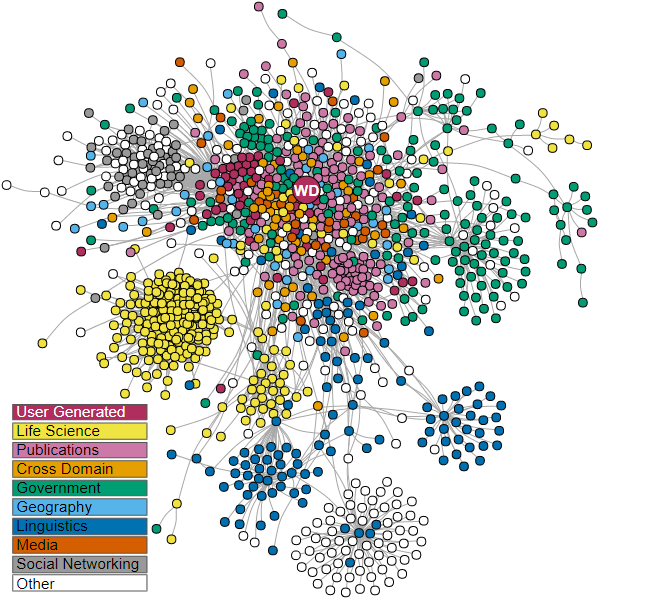
\includegraphics{./intro/bucketsAndBalls/Wikidata_in_linked_open_data.png}}
	}
    \caption[Wikidata in the Linked Open Data Cloud]{Wikidata in the Linked Open Data Cloud. Databases indicated as circles (with wikidata indicated as \textit{WD}), with grey lines linking databases in the network if their data is aligned. See the wikipedia article: \href{https://en.wikipedia.org/wiki/Linked_data}{Linked data}. Wikimedia Commons / \href{https://commons.wikimedia.org/wiki/File:Wikidata_in_the_Linked_Open_Data_cloud_2020-08-20.svg}{Thomas Shafee}}
	\label{fig:Wikidata_in_linked_open_data}
\end{marginfigure}

What is a variable in SPARQL? Let it be something that needs to be filled with something. But how to imagine this ``that``? Something abstract is easier to imagine if connected with something physical and concrete. It is difficult to imagine the time, but as soon as we imagine a clock with hands, it becomes easier. We cannot imagine furniture in general, but everyone can imagine a chair. 

Another difficulty lies in formulating the query in SPARQL language. Although working with SPARQL helps to understand how the knowledge graph\sidenote[][*6]{\index{Computer Science!Knowledge Graph} Knowledge graph is a knowledge base that uses a graph-structured data model to integrate data. Knowledge graphs are often used to store interlinked descriptions of entities - objects, events, situations or abstract concepts works. Next, a knowledge graph will be built (Pic.~\ref{fig:Graph_pattern_in_basket_and_balls_notation}).}, the SPARQL query does not look like it. It is like with symbols in mathematics. ``5~doesn`t look like five, while ||||| is five''.

So how do you solve the problem of defining a variable and formulating a SPARQL query?

Imagine each SPARQL query as a graph of baskets and balls related to each other. 

Let variables be something that needs to be filled, but now a variable is an abstract concept. We need a physical container to fill it with things. We need baskets. And things are like balls. So let's imagine the execution of a query as filling baskets with balls.

Then the process of filling the graph with balls will look like in Pic.~\ref{fig:Query_as_filling_buckets_with_balls}. A bucket \textbf{?A} should be filled with those balls which have a relation \textbf{R} to ball \textbf{B}.

\begin{marginfigure}
	{
		\setlength{\fboxsep}{0pt}%
		\setlength{\fboxrule}{1pt}%
		\fcolorbox{gray}{gray}{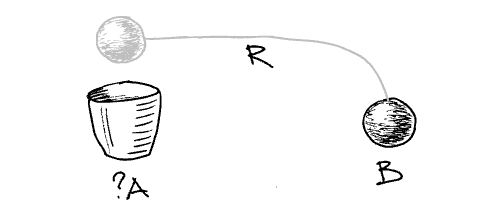
\includegraphics{./intro/bucketsAndBalls/graphPattern.PNG}}
	}
    \caption{Sample graph of filling baskets with balls.}
	\label{fig:Query_as_filling_buckets_with_balls}
\end{marginfigure}

The drawing will be clearer if we simplify it and draw a straight line (Pic.~\ref{fig:Graph_pattern_in_basket_and_balls_notation}). This is a graph pattern in Buckets`n`Balls notation. The direction of the relation R is not shown but it`s always from left to right.

\newpage
The process of writing and running a SPARQL query would then go through the following steps:
\begin{enumerate}
    \item Select your buckets (in them you are going to gather the balls you want).
    \item Compose your conditions as a graph of buckets and balls.
    \item Run your query to fill your buckets with balls.
\end{enumerate}

\begin{marginfigure}[-3cm]
	{
		\setlength{\fboxsep}{0pt}%
		\setlength{\fboxrule}{1pt}%
		\fcolorbox{gray}{gray}{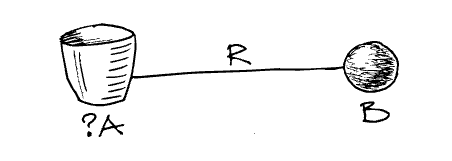
\includegraphics{./intro/bucketsAndBalls/graphPatternBucketsBalls.PNG}}
	}
    \caption{Graph pattern in Buckets`n`Balls notation.}
	\label{fig:Graph_pattern_in_basket_and_balls_notation}
\end{marginfigure}

Now we will write a request to, for example, get all the heads of the regions of Russia by following these steps:

\begin{enumerate}
    \item Let's take two baskets, one for regions and one for heads.
    \item We will tie the basket for regions to the ball ``region of Russia`` with the relation ``instance`` (instance of). Then from the set of balls~--- objects of Wikidata~--- only those balls that are the region of Russia will fall into this basket. The basket for regions is connected to the basket ``head` by the relation ``has a head``, in our case it will be the governor or the head of the region.
\end{enumerate}

Let`s make the request more interesting and add another basket for photos of governors. Now the query in the notation ``Buckets`n`Balls`` will be as in Pic.~\ref{fig:Query_in_basket_and_balls_notation}.

\begin{figure}[h!]
    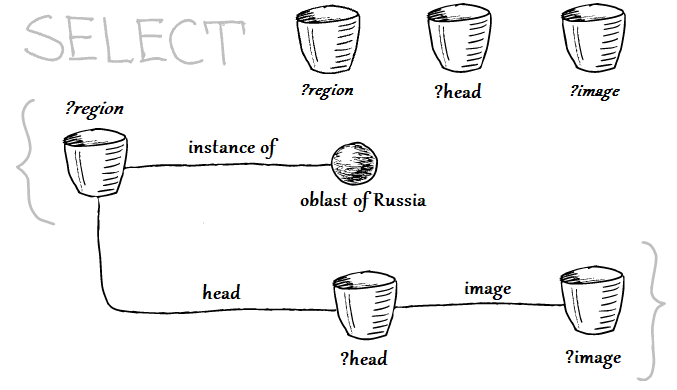
\includegraphics{./intro/bucketsAndBalls/Query_in_basket_and_balls_notation.PNG}
    \caption{Query in the notation ``Buckets`n`Balls`` to fill the baskets with ``region`` balls ``region of Russia``, ``head``~--- governors or heads of the region, ``image``~--- their photos.}
	\label{fig:Query_in_basket_and_balls_notation}
\end{figure}

After running the request (Pic.~\ref{fig:Query_in_basket_and_balls_notation}) our baskets will look like in Pic.~\ref{fig:3_buckets_region_head_image}.

\begin{marginfigure}
	{
		\setlength{\fboxsep}{0pt}%
		\setlength{\fboxrule}{1pt}%
		\fcolorbox{gray}{gray}{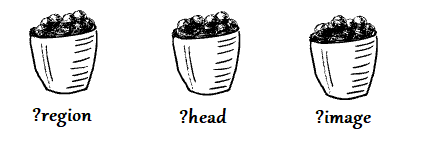
\includegraphics{./intro/bucketsAndBalls/3_buckets_region_head_image.PNG}}
	}
    \caption{Baskets after running the request in Pic.~\ref{fig:Query_in_basket_and_balls_notation}. \textit{?region} these are the regions of Russia, \textit{?head} these are the heads, \textit{?image}~--- these are photos of heads.}
	\label{fig:3_buckets_region_head_image}
\end{marginfigure}

Now let`s go to the service \href{https://query.wikidata.org/}{Wikidata Query Service} (next WDQS\sidenote[][]{See the explanations about WDQS at p.~\pageref{ch:review-wd}.}) and we will write this query in SPARQL. First, we will select and name the baskets to fill as follows:

\begin{lstlisting}[ language=SPARQL, numbers=none]
SELECT DISTINCT ?region ?head ?image
\end{lstlisting}

Next, we will write the conditions for matching balls to baskets. All conditions in SPARQL should be enclosed in curly brackets, as in Pic.~\ref{fig:Query_in_basket_and_balls_notation}.

Whenever we need a specific relation or ball, we need to use their identifiers. Wikidata makes it easy to find an identifier and suggest it when you select a relation (property) or ball (object) by its name (label). To indicate relationships in the Wikidata knowledge graph, we use the \textit{wdt:} prefix, and for objects (our balls)~--- the \textit{wd:} prefix. 

Following our notation (Pic.~\ref{fig:Query_in_basket_and_balls_notation}), we will write conditions for filling the first basket \textit{?region}, then we will write the first relation. Since the common part of direct relationship identifiers is wdt, we write \textit{wdt:} and then, in the WDQS service, press Ctrl+Space to start the Wikidata hint or autocomplete service (Pic.~\ref{fig:WDQS_popup_instance_of}). 

\begin{marginfigure}[-2cm]
	{
		\setlength{\fboxsep}{0pt}%
		\setlength{\fboxrule}{1pt}%
		\fcolorbox{gray}{gray}{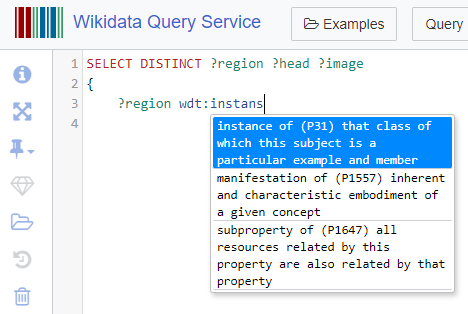
\includegraphics{./intro/bucketsAndBalls/WDQS_popup_instance_of.PNG}}
	}
    \caption{Using the Ctrl+Space command, the drop-down context menu for autofill Wikidata properties opened.}
	\label{fig:WDQS_popup_instance_of}
\end{marginfigure}

After that, we will reproduce the model from Pic.~\ref{fig:Query_in_basket_and_balls_notation} in a real SPARQL query.

Usually, when writing a SPARQL query, it is presented as a table with three columns: subject, predicate, object, or in the Wikidata language~--- object, property, value.

Perhaps a beginner programmer will find it easier to master SPARQL if at least your first queries resemble a graph. Let's try to take the graph in Pic.~\ref{fig:Query_in_basket_and_balls_notation} and write a SPARQL query in the most similar way (listing~\ref{lst:linkRegionsOfHeads}).

\begin{lstlisting}[ language=SPARQL, numbers=none, caption={List of heads of regions of Russia with photos. 
                    Received 44 references to the regions of Russia and their heads of government. 
                    Link to SPARQL query: \href{https://w.wiki/4NVc}{https://w.wiki/4NVc}},
                    label=lst:linkRegionsOfHeads]
SELECT DISTINCT ?region ?head ?image
{
    ?region wdt:P31 wd:Q835714; # oblast of Russia
            wdt:P6  ?head. # heads of government
    ?head  wdt:P18 ?image. # images of heads of government
}
\end{lstlisting}

Now look at how this request looks in the WDQS service, and run it. Then click on the eye icon on the left and select \textit{``image grid``} (Pic.~\ref{fig:WDQS_drop_down_result_type}) to view the results as an image grid.

\begin{marginfigure}[-1cm]
	{
		\setlength{\fboxsep}{0pt}%
		\setlength{\fboxrule}{1pt}%
		\fcolorbox{gray}{gray}{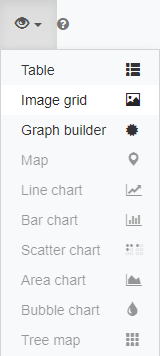
\includegraphics[width=0.5\linewidth]{./intro/bucketsAndBalls/WDQS_drop_down_result_type.PNG}}
	}
    \caption{Selecting the display of results as \textit{``image grid``}.}
	\label{fig:WDQS_drop_down_result_type}
\end{marginfigure}

This is not bad for the first result, but now under each photo we see only the IDs of people and areas. If we click on the ID hyperlink, we will get a lot of information about this object. But it would be clearer to specify the names of people and the names of areas (labels) in addition to identifiers as a result of the request. It`s like putting labels on our baskets (Pic.~\ref{fig:Query_in_basket_and_balls_notation_with_ids}).

\begin{figure}[h!]
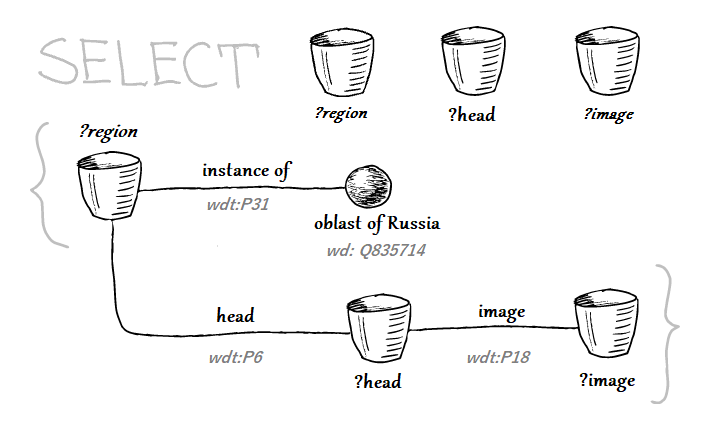
\includegraphics{./intro/bucketsAndBalls/Query_in_basket_and_balls_notation_with_ids.png}
\caption{A query in the notation ``Buckets`n`Balls`` with the numbers of properties and objects of Wikidata.}
\label{fig:Query_in_basket_and_balls_notation_with_ids}
\end{figure}

A label is something that every ball has, that is, a Wikidata object. A label is a name that allows you to distinguish objects from each other. Wikidata has a service that simplifies the output of labels on request. To do this, just add the word \textit{"Label"} to the end of the variable name and call the desired service. To call this service, type Ctrl + space on a new line inside curly brackets and when you start writing the word \textit{"Label"}, then a line with this service will be added\sidenote[][]{An example of calling this service is provided in listing ~\ref{lst:regionsOfHeads}}. By default, you get a hint with the interface language and English as an alternative if the label is not available in the language of the selected Wikidata interface.

Wikidata is full of such wonderful services, and for the final request we will use another one. To get the result immediately in the form of a set of photos of the heads of the regions, without additional clicking on the eye icon, place the following construction for WDQS somewhere in your request:
\begin{lstlisting}[ language=SPARQL, numbers=none ]
#defaultView:ImageGrid
\end{lstlisting}

In fact, not everything needs to be written manually. When you start typing, the autofill service will offer options.

Our last request is presented on the listing ~\ref{lst:regionsOfHeads}. A fragment of the result of its running is shown in Pic.~\ref{fig:Result_of_the_request}.

\begin{lstlisting}[ language=SPARQL, caption={List of heads of regions of Russia. 
                    Received 44 references to the regions of Russia and their heads of government. 
                    Link to SPARQL query: \href{https://w.wiki/4bGf}{https://w.wiki/4bGf}},
                    label=lst:regionsOfHeads, ]
# List of regions of the Russia and images of heads of government
#defaultView:ImageGrid
SELECT DISTINCT ?region ?regionLabel ?head ?headLabel ?image
{
  ?region wdt:P31 wd:Q835714; # ?region is Oblast of Russia
          wdt:P6  ?head.      #         has head of government
  ?head  wdt:P18 ?image.      # head has image
  SERVICE wikibase:label {bd:serviceParam wikibase:language "en"} 
}
\end{lstlisting}

\begin{figure}[h!]
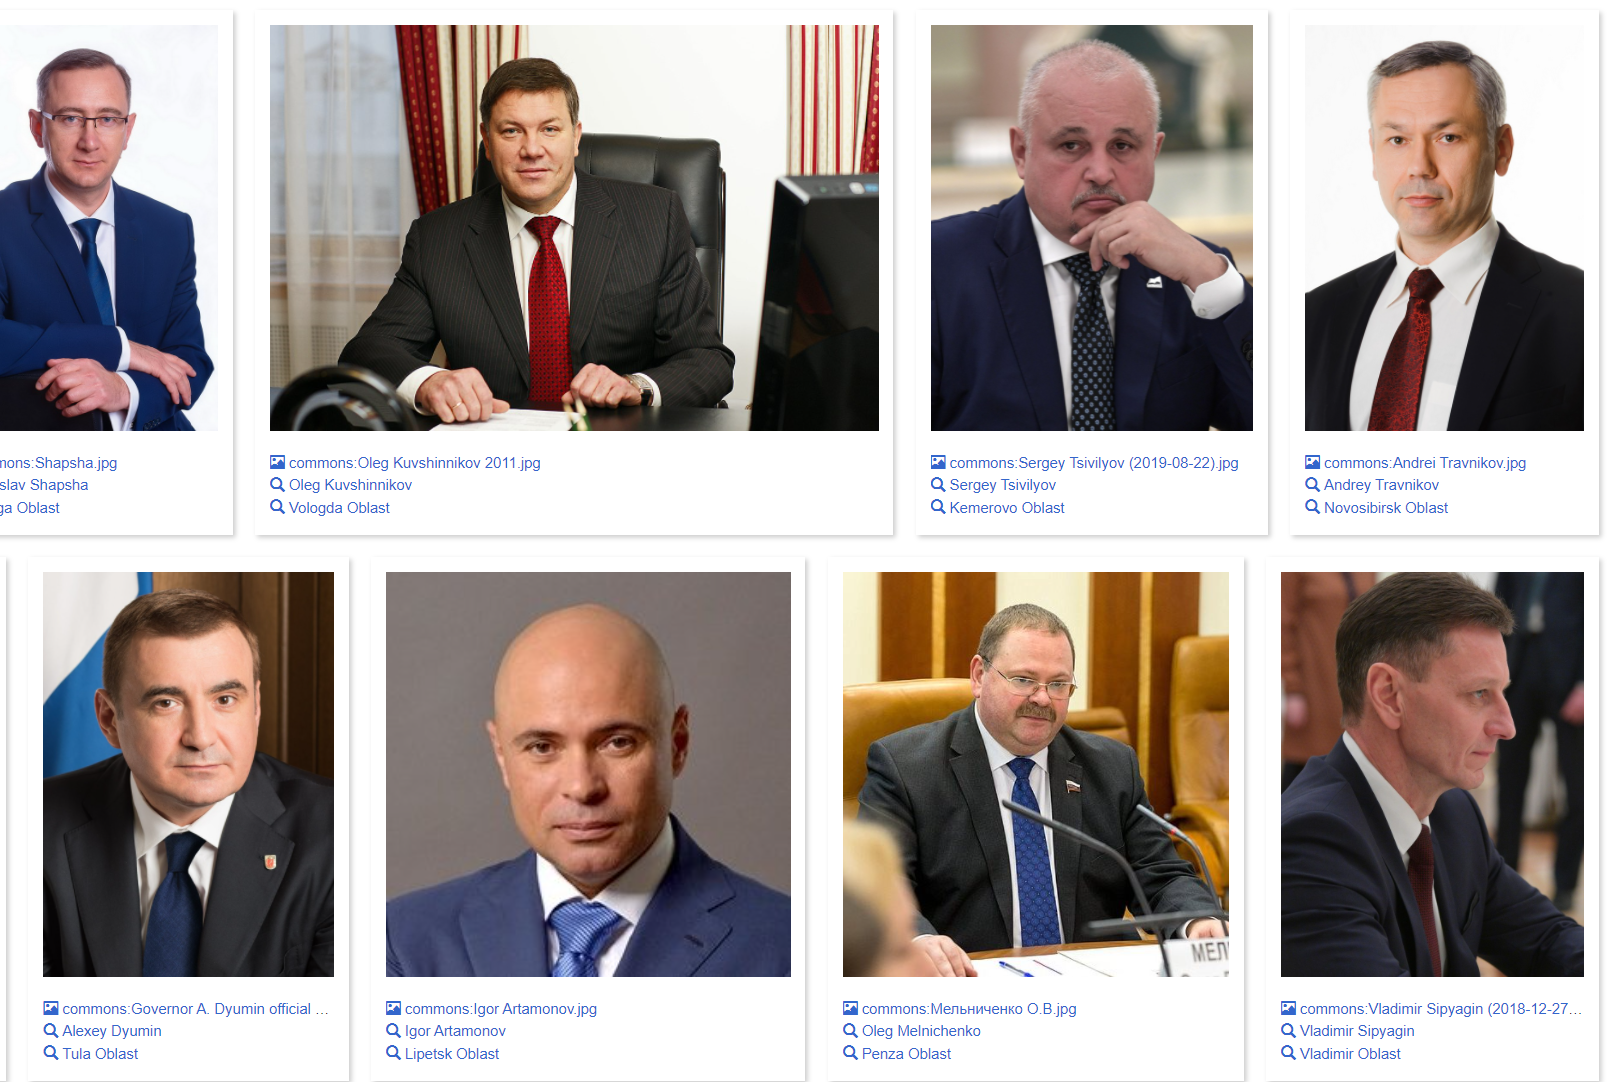
\includegraphics{./intro/bucketsAndBalls/result_of_request_for_photos_of_heads_of_government_en.png}
\caption{The result of the request in the form of a grid of images.}
\label{fig:Result_of_the_request}
\end{figure}

Thinking of SPARQL queries as linked baskets and balls can be helpful, at least at the beginning of the development of Wikidata. And, of course, every metaphor has its limitations. For example, you can't put the same ball in two different real baskets, but in these virtual~--- you can. <<Baskets and balls>> can be useful to climb to the height of the abstraction of Wikidata.



\pagelayout{wide} % No margins
\addpart{Wikidata for experts: \\ Bots}
\pagelayout{margin} % Restore margins

\chapter{Bots in Wikidata}
\label{ch:bots eng}

This chapter examines the automation of processes in Wikidata. On many occasions we want to correct recurring errors or enter large amounts of data in Wikidata instead of modifying properties one by one. 
For data entry we have at our disposal several tools that facilitate our work, such as OpenRefine\sidenote[][-58pt]{%
%
OpenRefine is an open-source desktop application for data cleanup and transformation to other formats. 
Since 2021 the program is avaliable to Wikipedia editors as an online-service. \url{https://openrefine.org/}%
} %
 or QuickStatements\sidenote[][0pt]{%
%
QuickStatements is a tool that can edit Wikidata items, based on a simple set of text commands. \url{https://quickstatements.toolforge.org/}%
%
}, but repetitive modifications and insertions over time should be done with a bot.


\section{Requirements}%
\label{sec:requirements}
We can program a bot in several programming languages, but to facilitate our task we can use Pywikibot, a collection of tools programmed in Python to facilitate access to information in Wikimedia Foundation projects. We have three options to run our programs:
\begin{enumerate}
%  \setlength{\itemindent}{2em}
  \item using a web shell like PAWS\sidenote[][-48pt]{PAWS (a web shell)~--- a Jupyter notebook deployment hosted by Wikimedia.}; 
  \item setting up a cloud infrastructure like Toolforge\sidenote[][-24pt]{Toolforge is a hosting environment for developers working on services that provide value to the Wikimedia movement \url{https://wikitech.wikimedia.org/wiki/Portal:Toolforge}};
  \item running it on our own computer.
\end{enumerate}

Any of the three options can be used 
thanks to the explanations 
we have in the official documentation\sidenote[]{See installation guide Pywikibot: \url{https://w.wiki/4CsU}}. 
If we use our own computer we must install Python, following the instructions in the documentation.
After the installation we can check 
if it is installed correctly 
by command \lstinline|python --version| 
in the Windows command prompt or in the Linux console (from now on everything must be done from here), 
and it will show us the version we are going to work with. 
Then we must install Pywikibot and configure it.

This configuration has several steps:
\begin{itemize}
  \setlength{\itemindent}{2em}
  \item Execute the following command to create the configuration file: \lstinline|py pwb.py generate_user_files|.
  \item Execute the following command to login: \lstinline|py pwb.py login|.
  \item Review the files \lstinline|user-config.py| and \lstinline|user-password.py| where we can indicate the user names that will make the modifications.
\end{itemize}

To view information or perform small tests we can use our username, but in case of making many modifications in Wikidata it is recommended to create a bot account and ask for permission to run it. To have this flag it is usually required to have some knowledge of editing in Wikimedia projects, which will certify that we will not make serious mistakes and we have the support of other users.

Normally to obtain this flag we will be asked to perform a specific number of test editions, to certify that such changes make sense, since we should have a low or zero error rate. We could also perform tasks with our user account, but with a low rate of edits.


\section{Our first scripts}
\label{sec:firstScript}

Once we have correctly configured Pywikibot we can run our first script~\ref{lst:page-get-eng}. 
We will go to the folder where Pywikibot is located and there we create a new file called \lstinline|test.py|.

We can edit the file with any text or code editor such as Visual Studio Code, Notepad++ or a simple Notepad.
Once inside the file we will put the following lines of code~\ref{lst:page-get-eng}.

\marginnote[*-6]{There are two rivers with the same name, which is ``Obnitsa'', one of them is in Poland, while the another in Serbia. Objects with the same names are easily distinguishable by identifiers in Wikidata: \wdqName{Obnitsa}{16583338} and \wdqName{Obnitsa}{959190}.}
%
\renewcommand{\lstlistingname}{Listing} % Query->Listing
\begin{lstlisting}[ language=Python,
                    caption={Receiving the content of the Wikidata page about the Obnitsa River in Poland},
                    label=lst:page-get-eng
                  ]
import pywikibot
site=pywikibot.Site('wikidata', "wikidata")
page=pywikibot.Page(site, u"Q16583338")     # river in Poland
print(page.get())
\end{lstlisting}
\renewcommand{\lstlistingname}{Query} % Listing->Query

We save the file and execute it by typing the following instruction: \lstinline|py pwb.py test.py|.

If everything has worked correctly we will be seeing in our console all the text written in the Obnica river article \wdqName{Obnitsa}{16583338} in Wikidata. 
In the first line of code~\ref{lst:page-get-eng} we have imported \lstinline|Pywikibot|. 
Then we have indicated the name of the project we want to work on, as we could do it in any Wikipedia language or Commons. Then we indicate a specific element, and finally we tell it that we want to get all the content.


``Page''~--- is a module that contains many methods that can be useful to us\sidenote[][-14pt]{%
%
To learn more about it we can go to the official documentation \url{https://doc.wikimedia.org/pywikibot/master/_modules/pywikibot/page.html}}. 
%
In addition to the \lstinline|get()| method, we have at our disposal the possibility of knowing the title of the element using the \lstinline|title()| method~(listing~\ref{lst:page-title}).

\begin{lstlisting}[ language=Python,
                    numbers=none,
                    caption={Receiving a header of the object with Q16583338 number},
                    label=lst:page-title
                  ]
import pywikibot
site=pywikibot.Site('wikidata', "wikidata")
page=pywikibot.Page(site, u"Q16583338")     # river in Poland
print(page.title())
\end{lstlisting}

We can also find out if this element is a redirect page with the \lstinline|isRedirectPage()| method. 
For it we are going to change the previous element and we are going to indicate another one  
(\href{https://www.wikidata.org/w/index.php?title=Q16583333&redirect=no}{Obnitsa (Q16583338)}) that is a redirect page (listing~\ref{lst:is-redirected}).

\begin{lstlisting}[ language=Python,
                    numbers=none,
                    caption={Receiving an answer to the question if an element is a redirect page (true or false)},
                    label=lst:is-redirected
                  ]
import pywikibot
site=pywikibot.Site('wikidata', "wikidata")
page=pywikibot.Page(site, u"Q16583333")
print(page.title())
print(page.isRedirectPage())
\end{lstlisting}

Caution: so far, the exercises were very simple, but as we progress we have to be careful with tabs, which let Python know what information goes inside the control structures.

The previous exercise~(listing~\ref{lst:is-redirected}) only returns true or false, but the usual use of this method is to ask if it is a redirect page or not, and act accordingly, warning the user that this element is a redirect page, as in the following example~(listing~\ref{lst:attention}).

\begin{lstlisting}[ language=Python,
                    numbers=none,
                    caption={Warning a user that the object is a redirect page},
                    label=lst:attention
                  ]
import pywikibot
site=pywikibot.Site('wikidata', "wikidata")
page=pywikibot.Page(site, u"Q16583333")    # redirect page
if (page.isRedirectPage()):
  print("Attention, this is a redirect, not an element")
\end{lstlisting}

But, what happens if we are analyzing several elements and we find one that does not exist? Possibly our program would return several errors because it could not analyze the interior of the element. For this, we can catch the errors in Python, but we can also ask if the element exists or not (listing~\ref{lst:page-exists}).

\begin{lstlisting}[ language=Python,
                    numbers=none,
                    caption={Check if the element exists or not},
                    label=lst:page-exists
                  ]
import pywikibot
site=pywikibot.Site('wikidata', "wikidata")
page=pywikibot.Page(site, u"Q107043778")    # non-existent object
if not page.exists():
  print("Sorry, but this element does not exist!")
\end{lstlisting}
\marginnote[-2.0cm]{Find how we can capture errors in Python and improve the previous program~\ref{lst:page-exists} so that we can capture possible errors returned by the program.}

Next, we are going to analyze an element in more depth, to know all those properties that it has included. To do this we can use the \lstinline|properties()| method, as we describe here (listing~\ref{lst:page-properties}).

\begin{lstlisting}[ language=Python,
                    numbers=none,
                    caption={Receiving the list of object properties},
                    label=lst:page-properties
                  ]
import pywikibot
site=pywikibot.Site('wikidata', "wikidata")
page=pywikibot.Page(site, u"Q16583338")     # river in Poland
print(page.properties())
\end{lstlisting}

When executing this script~\ref{lst:page-properties}, we can see that this method \lstinline|properties| 
returns a Python dictionary, and that is because the method returns a dictionary with the properties contained in that element. 
For example, we can see that in the property \lstinline|page_image_free| we get the picture that appears in the element, that
 \lstinline|wb_claims| contains the amount of properties that are entered in the element, 
or that \lstinline|wb_sitelinks| tells us the amount of links that exist to the rest of the Wikimedia Foundation projects.

The \lstinline|contributors()| method also returns a dictionary. In this case with the number of users who have contributed to the element. 
It will show us the user name of all the contributors, as well as the number of editions of each one.
We also have the method \lstinline|revision_count|, which returns the number of edits that have been made in total on the element, as shown below~\ref{lst:contributors-revision}.

\begin{lstlisting}[ language=Python,
                    numbers=none,
                    caption={Making a list of Wikidata object editors and an amount of fixes},
                    label=lst:contributors-revision
                  ]
import pywikibot
site=pywikibot.Site('wikidata', "wikidata")
page=pywikibot.Page(site, u"Q16583338")     # river in Poland
print(page.contributors())
print(page.revision_count())
\end{lstlisting}

There are other methods, which return more complex information than a data dictionary, such as an object.
This is the case of the \lstinline|linkedPages| method. If we use it as up to now (listing~\ref{lst:for-loop}) it will return: 
\lstinline|<pywikibot.data.api.PageGenerator object at 0x000002C6C7DB2FD0>|, indicating that it contains an object of type \lstinline|PageGenerator|. 
To be able to read it we can do it with a loop \lstinline|for| loop (listing~\ref{lst:for-loop}).

\begin{lstlisting}[ language=Python,
                    numbers=none,
                    caption={Reading an object of type \lstinline|PageGenerator|},
                    label=lst:for-loop
                  ]
import pywikibot
site=pywikibot.Site('wikidata', "wikidata")
page=pywikibot.Page(site, u"Q16583338")     # river in Poland
for linked in page.linkedPages():
  print(linked)
\end{lstlisting}

As we can see the \lstinline|page.linkedPages()| method provides us with the links to which we can click from the element. 
First, the elements will be shown and then the properties (including the information found in the references). Obviously if the selected element is not very large, the number of links will not be very large, but if we try this example with a very large element, the number of links will be very large.

To know the number of elements that are linking to a specific one,
we also have a method called \lstinline|backlinks()|, which contains an object and that we have to go through as we did in the previous exercise (listing~\ref{lst:for-loop}).

Depending on the element we may find an empty list, so we will select an element that is linked to other elements (listing~\ref{lst:back-links}).

\begin{lstlisting}[ language=Python,
                    numbers=none,
                    caption={Using method \lstinline|backlinks()| for receiving objects that referring to the specified object},
                    label=lst:back-links
                  ]
import pywikibot
site=pywikibot.Site('wikidata', "wikidata")
page=pywikibot.Page(site, u"Q6980876")     # river in Spain
for links in page.backlinks():
  print(links)
\end{lstlisting}

In this case we have chosen another river (\wdqName{Pisueña}{6980876}), 
which is linked twice: by \wdqName{another river}{14360} and by a \wdqName{redirect page}{23993869}. 
In this way we can know the number of times a certain element (Pisueña) is being linked.

\marginnote[0.0cm]{Exercise: Put into practice everything we have seen so far but using an element with a low number, which probably has much more information entered than the examples we have used so far.}

In addition to the \lstinline|Page| module Pywikibot provides us with many other possibilities. 
For example, introducing a single element does not make much sense, normally we will want to work with several elements to analyze them and if necessary modify them. For this we can make use of the queries that we have been doing throughout the course.


\section{Running queries}
\label{sec:running queries eng}

First, we go to Wikidata Query Service \href{https://query.wikidata.org/}{WDQS}\footnote{%
See explanations of WDQS on the page~\pageref{sect:WDQS}.%
}%
 to create our query. 
We look for possible errors in the data entered, such as people who have a certain country in the property \wdProperty{17}{country}.
This is a common error as many users enter \wdProperty{17}{country} instead of property \wdProperty{27}{country of nationality}.
This query could look like this~(listing~\ref{lst:bug-finding}).

\begin{lstlisting}[ language=SPARQL,
        numbers=none,
        caption={\href{https://w.wiki/https://w.wiki/4cBg}{Query for receiving list of users who mistakenly entered country instead of country of nationality}\protect\footnotemark},
        label=lst:bug-finding
                  ]
SELECT ?item ?itemLabel WHERE 
{
  ?item wdt:P31 wd:Q5;  # instance of human
        wdt:P17 wd:Q36. # has country Poland
  SERVICE wikibase:label {bd:serviceParam wikibase:language "en"}
}
\end{lstlisting}
\footnotetext{Received 3 occupations in 2021. Link to SPARQL-query: \href{https://w.wiki/4cBg}{https://w.wiki/4cBg}}

We must check if the query~\ref{lst:bug-finding} returns any value,
since it could be that there are no errors to be solved. 
In that case we can change the country 
(for example, we can indicate the following country (Q37~--- Lithuania), instead of the checked one (Q36~--- Poland)), 
since there will surely be other countries with the same error.

When we get a query~\ref{lst:bug-finding} that returns any person, 
we can add the query to our program, like this~\ref{lst:identify-bugs}.

% caption=[Identification of users with a country-citizenship error]{Inclusion of a SPARQL-query for identification of users with a country-citizenship error using an example of Poland (Q36) to a Python program, with the output of the usernames of all such users}
\begin{lstlisting}[ language=Python,
    numbers=none,
    caption={Identification of users with a country-citizenship error using an example of Poland(Q36) (inclusion of a SPARQL-query to a Python program)},
    label=lst:identify-bugs
    ]
import pywikibot
from pywikibot import pagegenerators
site=pywikibot.Site('wikidata', "wikidata")
query = """
  SELECT DISTINCT ?item WHERE {
    SERVICE wikibase:label {bd:serviceParam wikibase:language "en"}
    ?item wdt:P31 wd:Q5.
    ?item wdt:P17 wd:Q36.
  } """

pages = pagegenerators.WikidataSPARQLPageGenerator(query,site=site)
for item in pages:
  print(item.title())
\end{lstlisting}    

With respect to the previous exercises we have only imported the \lstinline|pagegenerators|, a module that allows us to generate a list of items from certain filters as a SPARQL query as above (listing~\ref{lst:bug-finding}). We have saved the query in a variable called /textit{query}, and then we have passed it to the pagegenerators method called \textit{WikidataSPARQLPageGenerator()}. The data returned by this method has been traversed with a for loop and we have displayed the title of the item.

In short, this program (~(listing~\ref{lst:identify-bugs})) shows us all the people who have Poland as a country.

We can already obtain several elements at the same time. Now it is time to delve into the content of these. Instead of displaying the title of the article, we will display some parts of its content. For example, sitelinks, aliases, labels or claims~(listing~\ref{lst:display-linkslabels}).

\begin{lstlisting}[ language=Python,
                    numbers=none,
                    caption={Displaying sitelinks, aliases, labels, claims},
                    label=lst:display-linkslabels
                  ]
import pywikibot
from pywikibot import pagegenerators
site=pywikibot.Site('wikidata', "wikidata")
query = """
  SELECT DISTINCT ?item WHERE {
    SERVICE wikibase:label {bd:serviceParam wikibase:language "en"}
    ?item wdt:P31 wd:Q5.
    ?item wdt:P17 wd:Q36.
  } """

pages = pagegenerators.WikidataSPARQLPageGenerator(query, site=site)
for item in pages:
  item.get()
  print(item.sitelinks)
  print(item.aliases)
  print(item.labels)
  print(item.claims)
\end{lstlisting} 

\marginnote[0.0cm]{Exercise: test the queries you have performed earlier in the course and display the results in your console with messages to help you know what is running.}

We have shown the information in the Wikidata elements, but now let's see how we can modify them. 

\section{Modifying the values entered in Wikidata}
\label{sec:modifying the values entered in Wikidata eng}

The search for errors that are repeated over time is one of the tasks of a bot programmer, because depending on the task performed by the bot, it will have to be executed regularly, and improve the search for errors over time. For example, the following query returns all professions sorted by the number of times they are being used in Wikidata~(listing~\ref{lst:occupation-list}).

\begin{lstlisting}[ language=SPARQL,
                    numbers=none,
                    caption={\href{https://w.wiki/4bLo}{List of occupations sorted by the their use amount in Wikidata}\protect\footnotemark},
                    label=lst:occupation-list
                  ]
SELECT ?instanceLabel ?value WHERE {
  {
    SELECT ?instance (COUNT(DISTINCT ?item) AS ?value) 
    WHERE { ?item wdt:P106 ?instance. } #P106 - occupation
    GROUP BY ?instance
    ORDER BY DESC (?value)
  }
  SERVICE wikibase:label {bd:serviceParam wikibase:language "en"}
}
ORDER BY DESC (?value)
\end{lstlisting} 
\footnotetext{Returned \num{16979} occupations in 2021. Link to SPARQL-query: \href{https://w.wiki/4bLo}{https://w.wiki/4bLo}}

This query~\ref{lst:occupation-list} 
can be used to check which professions are being used incorrectly, or have been introduced by vandals.
Reviewing the list, we can see that there are some professions 
that are not correct and have meaningless information
such as \wdqName{Salinas de Ibargoiti}{7404672}, \wdqName{Order of Saint Basil the Great}{7319129}, \wdqName{Promoted to Glory}{7249866}, \wdqName{Princes}{7244433} and \wdqName{Point Loma Nazarene University}{7208069}. 
We can create a list of errors and show the biographies that have these professions entered~(listing~\ref{lst:occupation-mistakeslist}).

\begin{lstlisting}[ language=Python,
                    caption={Making a list of errors and displaying users with occupation errors},
                    label=lst:occupation-mistakeslist
                  ]
import pywikibot
from pywikibot import pagegenerators
site=pywikibot.Site('wikidata', "wikidata")
delete_occupation={"Q7404672", "Q7319129", "Q7249866", "Q7244433", 
"Q7208069"}
for occupation in delete_occupation:
  query = """
    SELECT DISTINCT ?item WHERE {
      SERVICE wikibase:label { bd:serviceParam wikibase:
language "en". }
      ?item wdt:P31 wd:Q5.     # P31 - instance of, Q5 - human
      ?item wdt:P106 wd:""" + occupation + """.
    } """

  pages=pagegenerators.WikidataSPARQLPageGenerator(query, site=site)
  for item in pages:
    print("Users whose occupation is
{occupation}: {title}" . format(occupation=occupation, 
title=item.title()))
\end{lstlisting} 
\marginnote[-2.0cm]{Attention: so far we had used \lstinline|print()| 
to show the information contained in the variables, 
but in the previous exercise~(listing~\ref{lst:occupation-mistakeslist})
we have used \lstinline|format()|, as it is recommended to give clarity to string.}

The list has been created in the variable \textit{delete\_occupation}. We run through it with a \textit{for} loop to call the query for each of the professions that we have been adding. This time the query~(listing~\ref{lst:occupation-mistakeslist}) is not the same as before~(listing~\ref{lst:occupation-list}), now it(~listing~\ref{lst:occupation-mistakeslist} has a variable \textit{occupation} that is modified depending on the value of \textit{delete\_occupation}. The query will ask for the people who have a profession that matches the value of \textit{delete\_occupation}, and will show it on the screen.

Now, if we are sure that this information is wrong and we want to delete it, we must indicate the specific property we want to delete.

The problem is that a biography could have three professions, and only one of them is the one we want to delete. We cannot delete all the values of the property, we have to know the specific data to delete. In the following~(listing~\ref{lst:delete-occupation}) we will see how this can be done. 

\begin{lstlisting}[ language=Python,
                    caption={Deleting an occupation},
                    label=lst:delete-occupation
                  ]
import pywikibot
from pywikibot import pagegenerators
site=pywikibot.Site('wikidata', "wikidata")
delete_occupation={"Q7404672", "Q7319129", "Q7249866", "Q7244433", 
"Q7208069"}
for occupation in delete_occupation:
  query = """
    SELECT DISTINCT ?item WHERE {
      SERVICE wikibase:label {bd:serviceParam wikibase:language "en"}
      ?item wdt:P31 wd:Q5.
      ?item wdt:P106 wd:""" + occupation + """.
    } """

  pages = pagegenerators.WikidataSPARQLPageGenerator(query, 
  site=site)
  for item in pages:
    print("These are users who have
{occupation} as their occupation: {title}" . format(occupation=occupation, 
title=item.title()))
    item.get()

    for valor in item.claims['P106']:
      if (str(valor.getTarget())=='[[wikidata:' + occupation + 
']]'):
        print("<<<<< Deleting {occupation} of {title} >>>>>" . 
format(occupation=occupation, title=item.title()))
        item.removeClaims(valor, summary=u'Deleting erroneous values in P106')
\end{lstlisting} 

In the previous code listing~\ref{lst:delete-occupation} what we have done is to maintain the previous code listing~\ref{lst:occupation-mistakeslist}, but adding the last lines, in which we go through the values contained in the property \wdProperty{106}{}, with the method \textit{claims}. If this one coincides with the occupation that we are looking for, we delete it with the method \textit{removeClaims}. This method needs the value we want to delete and the edit summary \sidenote[]{Commenting fixes allows other editors to easily understand what changes have been made to a page or Wikidata object.} to show the rest of the users what is being done.

Caution: this kind of edits can cause many problems on Wikidata and administrators may block your user account. Make few changes at the beginning, and always check the edit history to see what information has been modified.
\subsection{Exercises}

\begin{enumerate} 
\item Exercise: add more professions that are wrong in the variable \textit{delete\_occupation} and run the bot to perform the deletions of those properties.
\end{enumerate}



\pagelayout{wide} % No margins
\addpart{Examples with Wikidata objects}
\pagelayout{margin} % Restore margins

\setchapterimage[6cm]{chapter/aircraft/aircraft_title_photo2.jpg}
\setchapterpreamble[u]{\margintoc}
\chapter{Aircraft and their manufacturers\protect\footnotemark}
\labch{aircraft-chapter_en}

\footnotetext{\href{https://en.wikipedia.org/wiki/NASA_X-43}{NASA X-43} it is the fastest aircraft in the history of aviation.
Author: \href{https://commons.wikimedia.org/wiki/File:X43a2_nasa_scramjet.jpg}{NASA, WikiCommons / 2008 / Public Domain}. }

The chapter explores the various properties of aircraft based on the Wikidata database.
During the study, using SPARQL queries calculated on objects of the ``Aircraft" type, a list of aircraft and their manufacturers was obtained, the number 
produced aircraft for different models. For this number of aircraft, the \Wikiref{Pareto principle} has been verified by models.
A diagram is also obtained showing the ratio of the total number of aircraft manufacturers by country.
The chapter concludes with an estimate of the completeness of the data presented in Wikipedia and Wikidata. 
According to it, only 595 records of aircraft manufacturers from \num{1700} for 2020 are presented in Wikidata.
Assuming a fixed number of new aircraft manufacturers emerge each year and the number of Wikidata entries entered annually, 
we can assume that in about 75 years (that is, in 2095) Wikidata will contain records of all aircraft manufacturers.


%%%%%%%%%%%%%%%%%%%%%%%%%%%%%%%%%%%%%%%%%%%%%%%%%%%%%%%

\section{List of aircrafts}

Aircraft~--- an aircraft supported in the atmosphere by interaction with air, different from interaction with air reflected from the 
surface of the earth or water.
Aircraft include the following types of aircraft: gyroplane, balloon, helicopter, rotorcraft, airship, flywheel, glider and airplane.
Aircraft do not include spaceships, rockets, ekranoplanes (but not ekranoplanes) and hovercraft.

Let's build a list of all instances of the object ``Aircraft" \href{https://www.wikidata.org/wiki/Q11436}{Q11436}.

\begin{lstlisting}[ language=SPARQL, breaklines=true, 
                    caption={List of aircrafts.\\\hspace{\textwidth}
                        The result contains \num{1564} aircrafts in 2017, 
                        \num{3324} aircrafts in 2020.\\\hspace{\textwidth}
                        SPARQL query: \href{https://w.wiki/rez}{w.wiki/rez}
                        },
                    label=lst:aircraft_listing_1,
                    texcl 
                    ]
# List of aircrafts
SELECT ?plane ?planeLabel
WHERE
{
    ?plane wdt:P31 wd:Q11436. # instance of aircraft
    SERVICE wikibase:label {bd:serviceParam wikibase:language "en"}
}
\end{lstlisting}

The most complete and well-developed aircraft on Wikidata in 2017 were \href{https://www.wikidata.org/wiki/Q271446}{Mikoyan-Gurevich MiG-3}, 
\href{https://www.wikidata.org/wiki/Q1349098}{Yakovlev Yak-36}, \href{https://www.wikidata.org/wiki/Q429839}{Mitsubishi A5M}. 
As for 2020, the most complete and well-developed aircrafts on Wikidata are \href{https://www.wikidata.org/wiki/Q770863}{Sopwith Triplane} (18 properties), 
\href{https://www.wikidata.org/wiki/Q1658673}{IL-103} (14 properties), \href{https://www.wikidata.org/wiki/Q665071}{Martin 2-0-2} (14 properties).
%Almost empty and uninformative aircraft for 2017 turned out to be: \href{https://www.wikidata.org/wiki/Q464247}{Mikoyan-Gurevich MiG-1}, 
%\href{https://www.wikidata.org/wiki/Q2296502}{Sukhoi Su-6}, \href{https://www.wikidata.org/wiki/Q1658673}{Il-103}.
For 2020, uninformative aircraft are: \href{https://www.wikidata.org/wiki/Q820603}{Beriev Be-1} (Wikidata object has 3 properties), \href{https://www.wikidata.org/wiki/Q117984}{Lituanica} (Wikidata object has 4 properties), 
\href{https://www.wikidata.org/wiki/Q572762}{Lavochkin La-168} (Wikidata object has 3 properties).

%%%%%%%%%%%%%%%%%%%%%%%%%%%%%%%%%%%%%%%%%%%%%%%%%%%%%%%

\section{Aircraft manufacturers}

Let's make a list of aircraft manufacturers by completing the request~\ref{lst:aircraft_listing_2}.

\index{SPARQL!COUNT!Aircraft manufacturers}
\begin{lstlisting}[ language=SPARQL, breaklines=true, 
                    caption={Aircraft manufacturers\\\hspace{\textwidth}
                        The result contains \num{300} manufacturers in 2017, 
                        \num{597} manufacturers in 2020.\\\hspace{\textwidth}
                        SPARQL query: \href{https://w.wiki/vNn}{w.wiki/vNn}
                        },
                    label=lst:aircraft_listing_2,
                    texcl 
                    ]
# Count aircraft having property manufacture, group by manufacture
SELECT ?manufacture ?manufactureLabel (COUNT(?plane) AS ?count) 
WHERE {
  ?plane wdt:P31 wd:Q11436. # instance of aircraft
  ?plane wdt:P176 ?manufacture. # show manufacture
  SERVICE wikibase:label {bd:serviceParam wikibase:language "en".}
}
GROUP BY ?manufacture ?manufactureLabel
\end{lstlisting}

The result of the query~\ref{lst:aircraft_listing_2} is a list of all aircraft manufacturers.

%%%%%%%%%%%%%%%%%%%%%%%%%%%%%%%%%%%%%%%%%%%%%%%%%%%%%%%

\label{question:aircraft_manufacturers_en}
\marginnote{
Which of the Russian aircraft manufacturers below have websites?
\begin{itemize}
\item \Wikiref{Russian Aircraft Corporation MiG}
\item \Wikiref{Saratov Aviation Plant}
\item \Wikiref{Tupolev}
\item \Wikiref{Sukhoi}
\end{itemize}
The answer is on page~\pageref{answer:aircraft_manufacturers_en}.
}


\section{Number of aircraft produced}

\index{Aircraft!Aviation industry!definition}
The aviation industry is one of the largest mechanical engineering industries in the world. Its tasks include both the development 
and production of various aerial vehicles. In order to assess which aircraft models are the most widespread, we will build a diagram 
of the produced aircraft of various models, , shown in Fig.~\ref{fig:Number_of_aircraft_produced_en_2020}.
To get the number of aircraft produced, query~\ref{lst:aircraft_listing_3}.


\begin{lstlisting}[ language=SPARQL, breaklines=true, 
                    caption={Received \num{288} models, for which the number\\\hspace{\textwidth}
                        of aircraft produced, 2020 is known. 
                        SPARQL query: \href{https://w.wiki/v4J}{w.wiki/v4J}
                        },
                    label=lst:aircraft_listing_3,
                    texcl 
                    ]
# List of aircraft models, sorted by number of aircraft built
SELECT ?plane ?planeLabel ?planes_produced WHERE {
  ?plane wdt:P31 wd:Q11436. # instance of aircraft
  ?plane wdt:P1092 ?planes_produced.  # total aircraft manufactured
  SERVICE wikibase:label {bd:serviceParam wikibase:language "ru,en".}
}
ORDER BY DESC(?planes_produced)
\end{lstlisting}

Some aircraft models were produced in small numbers, so they can be excluded to improve the readability of the diagram~\ref{fig:Number_of_aircraft_produced_en_2020}. 
To get a new list, let's add a filter to the request~\ref{lst:aircraft_listing_4}.

\index{SPARQL!FILTER!List of aircraft manufactured over 10 pieces}
\begin{lstlisting}[ language=SPARQL, breaklines=true, 
                    caption={A list of \num{124} models, filtered by the\\\hspace{\textwidth}
                        number of aircraft produced, has been received.
                        SPARQL query: \href{https://w.wiki/v4N}{w.wiki/v4N}
                        },
                    label=lst:aircraft_listing_4,
                    texcl 
                    ]
# List of aircraft models, sorted by number of aircraft built
#defaultView:BarChart
SELECT ?plane ?planeLabel ?planes_produced WHERE {
  ?plane wdt:P31 wd:Q11436. # instance of aircraft
  ?plane wdt:P1092 ?planes_produced.  # total aircraft manufactured
  FILTER (?planes_produced > 10)
  SERVICE wikibase:label {bd:serviceParam wikibase:language "ru,en".}
}
ORDER BY (?planes_produced)
\end{lstlisting}

The figure in Fig.~\ref{fig:Number_of_aircraft_produced_en_2020} shows that the following aircraft models were produced the most in 
2020: \href{https://www.wikidata.org/wiki/Q2096452}{PA-32 Cherokee Six} (\num{7842} pieces), \href{https://www.wikidata.org/wiki/Q1860367}{Piper PA-24 Comanche} 
(\num{4857}), \href{https://www.wikidata.org/wiki/Q694521}{Junkers W 34} (\num{3000}), \href{https://www.wikidata.org/wiki/Q941011}{Pomilio PE} 
(\num{1616}).

\begin{figure*}[h]

    \setlength{\fboxsep}{0pt}%
    \setlength{\fboxrule}{1pt}%
    \fcolorbox{gray}{gray}{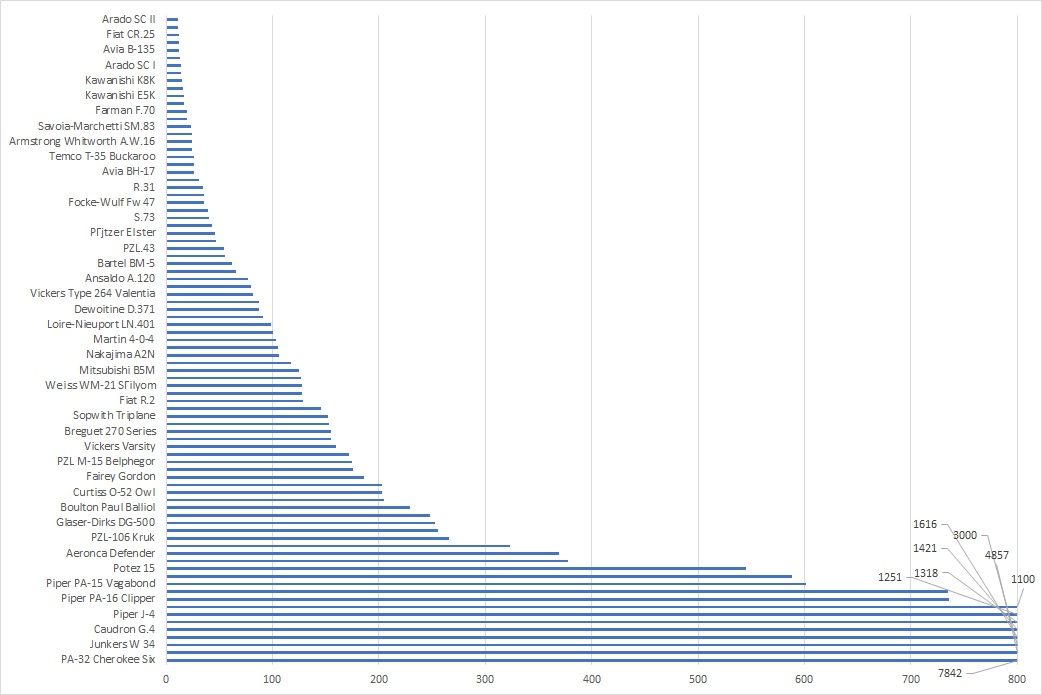
\includegraphics[width=\linewidth]{./chapter/aircraft/Number_of_aircraft_produced_en_2020.jpg}}%

	\caption[Number of aircraft produced by model, 2020.]{The number of aircraft produced by model, 2020. The diagram is built in Microsoft Excel based on the data obtained using the query ~\protect\ref{lst:aircraft_listing_4}.}%
    \label{fig:Number_of_aircraft_produced_en_2020}%
\end{figure*}

Now let's try to answer the question: ``Does \Wikiref{Pareto principle} hold with respect to the 
number of aircraft models"?

In order to build a graph, you must perform the following steps:

\begin{enumerate} 
  \item Calculate the total number of aircraft for all models using the script shown in the listing~\ref{lst:aircraft_listing_5}.

  \index{SPARQL!SUM / Total number of aircraft produced}
  \begin{lstlisting}[ language=SPARQL, breaklines=true,  
                      caption={Total number of aircraft produced\\\hspace{\textwidth}
                          The result contains \num{33 178} aircrafts in 2020.
                          SPARQL query: \href{https://w.wiki/rf9}{w.wiki/rf9}
                          },
                      label=lst:aircraft_listing_5,
                      texcl 
                      ]
  SELECT (SUM(?count) as ?sum) WHERE {
    SELECT ?count WHERE {
      SERVICE wikibase:label {bd:serviceParam wikibase:language "en".}
      ?plane wdt:P31 wd:Q11436; # instance of aircraft
			 wdt:P1092 ?count. # total aircraft manufactured
    }
  }
  \end{lstlisting}
  
  \label{question:aircraft_question_2}
  \marginnote{
	Find the correspondence between the date of foundation and the company in the following table:
	\\
	\begin{tabular}{ l | l }
	Company & Foundation date \\ \hline
	\Wikiref{MiG} & January 1, 1939 \\
	\Wikiref{Vympel NPO} & November 18, 1949 \\
	\Wikiref{Tupolev} & December 18, 1939 \\
	\Wikiref{Sukhoi} & January 1, 1922 \\
	\end{tabular}
	\\
	The answer is on page~\pageref{answer:aircraft_answer_2}.
  }
  
  \item The X axis represents the number of aircraft models under consideration (that is, for x = 1, we consider the number of aircraft of the first model 
  produced, for x = 2~--- the number of aircraft of the first and second model, and so on). 
  On the Y axis we will plot F(n) = $\sum\limits_{i=1}^n f(i)$, where f(i)~--- is the number of aircraft of model i released. 
  In this case, the condition f(i) > f(j) is satisfied, for i < j, where i, j~--- is the aircraft model number 
  (that is, the number of released aircraft models is pre-ordered in descending order). Also, on the X-axis, we postpone the second scale from 0 to 1, 
  to make it easier to determine the parameters for checking the implementation of \Wikiref{Pareto principle}.
  
\end{enumerate}



\begin{figure*}[h]

    \setlength{\fboxsep}{0pt}%
    \setlength{\fboxrule}{1pt}%
    \fcolorbox{gray}{gray}{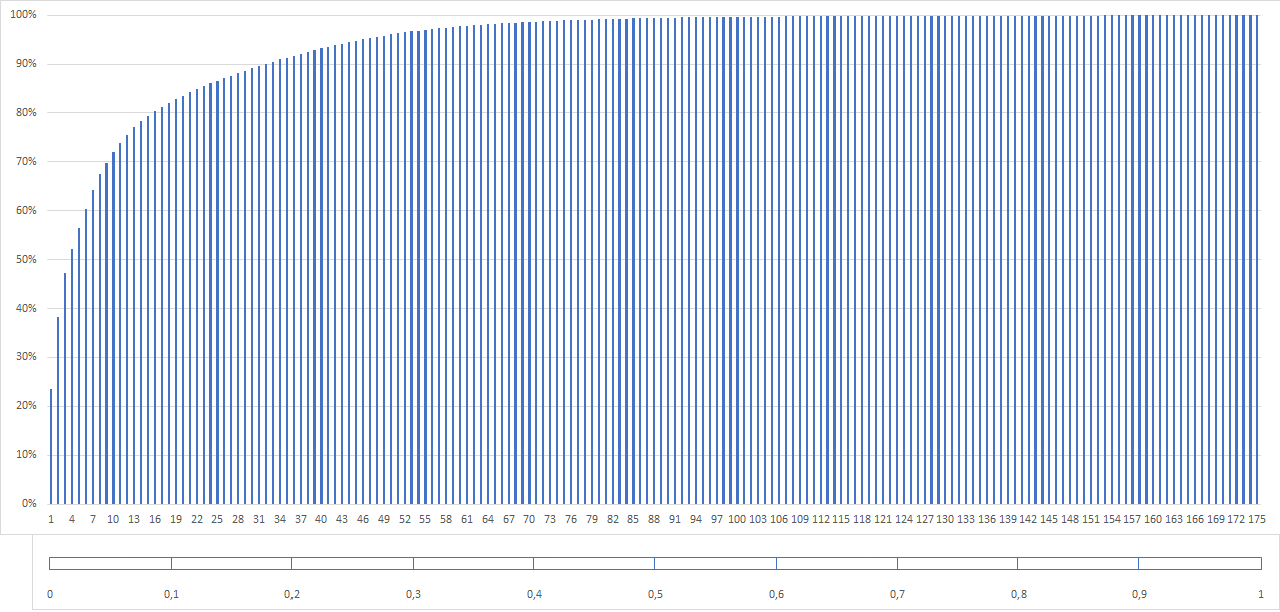
\includegraphics[width=\linewidth]{./chapter/aircraft/Pareto_principle_diargam_en.png}}%

%	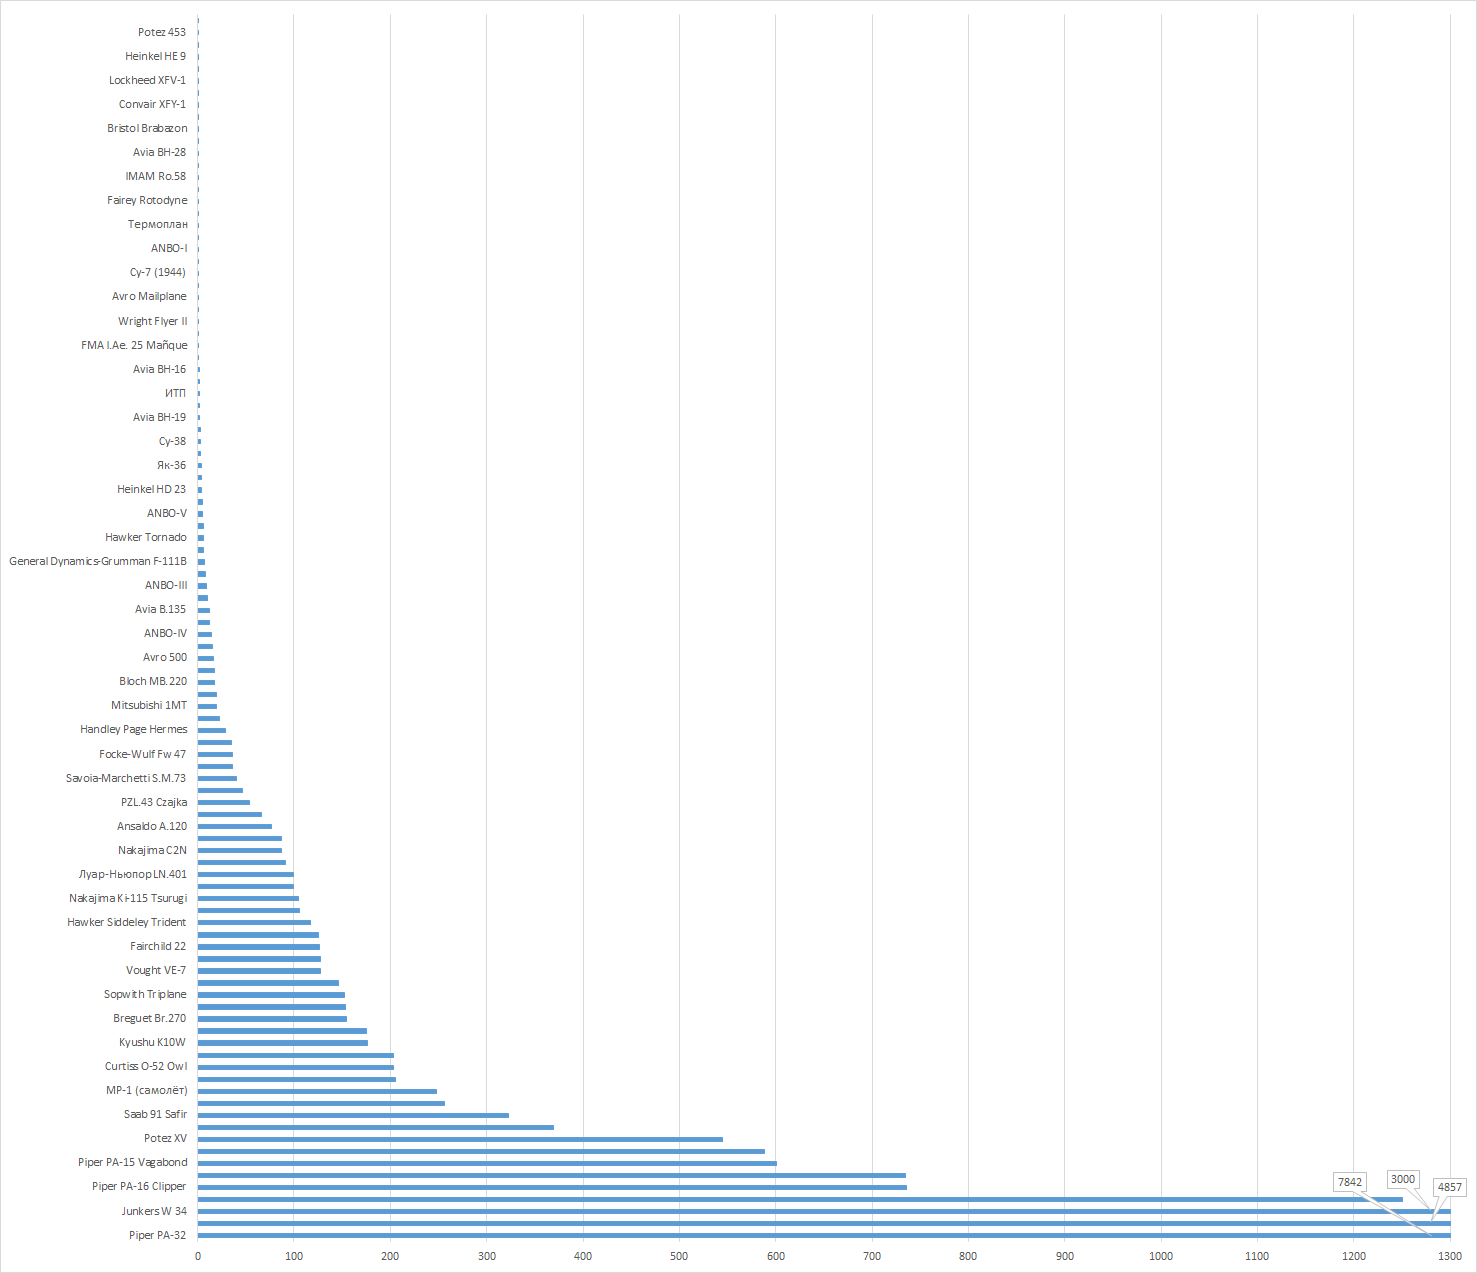
\includegraphics{chapter/aircraft/Number_of_aircraft_produced_ru.png}%
	\caption{Percentage of the number of aircraft models produced by all airlines to the total number of aircraft manufactured for all time, 2020.}%
    \label{fig:Pareto_principle_diargam_en}%
\end{figure*}

According to the graph~\ref{fig:Pareto_principle_diargam_en}, it can be seen that 80\% of all aircraft produced belong to 16 different aircraft 
models, which is 9.2\% of the total number of models. Pareto's law states that: ``20\% of the efforts give 80\% of the result, and the remaining 80\%
 of the efforts - only 20\% of the result." It can be concluded that a stronger law is fulfilled than the Pareto principle regarding the number 
 of aircraft models.

\label{question:aircraft_question_3}
\marginnote{
Find the correspondence between the location of the company's headquarters and the company.
\\
\begin{tabular}{ l | l }
Company & Headquarters \\ \hline
\Wikiref{Kazan Helicopters} & Kazan \\
\Wikiref{Saratov Aviation Plant} & Saratov \\
\Wikiref{Ulan-Ude Aviation Plant} & Ulan-Ude \\
\Wikiref{Sukhoi} & Moscow \\
\end{tabular}
\\
The answer is on page~\pageref{answer:aircraft_company_headquarters_en}.
}

%%%%%%%%%%%%%%%%%%%%%%%%%%%%%%%%%%%%%%%%%%%%%%%%%%%%%%%

\section{In which countries are aircraft produced}

Let's build a list of the number of aircraft manufacturers by country. To execute the query~\ref{lst:aircraft_listing_7}, we use the grouping 
by country (GROUP BY) and use the ``Count" function for each country to calculate the total number of aircraft manufacturing plants.

%\index{SPARQL!COUNT!List of the ratio of the number of manufacturers aircraft by country}
%\begin{lstlisting}[ language=SPARQL, breaklines=true, 
%                    caption={List of the ratio of the \\\hspace{\textwidth} 
%						number of manufacturers aircraft by country\\\hspace{\textwidth}
%                        The result contains \num{39} records in 2017, 
%                        \num{46} records in 2020.\\\hspace{\textwidth}
%                        SPARQL query: \href{https://w.wiki/rfD}{w.wiki/rfD}
%                        },
%                    label=lst:aircraft_listing_6,
%                    texcl 
%                    ]
%# Count manufacture having property country group by country
%SELECT ?countryLabel (count(?manufacture) as ?count)
%WHERE
%{
%    ?manufacture wdt:P31 wd:Q936518. # instance of aerospace manufacture
%  	?manufacture wdt:P17 ?country. # belong to country
%    SERVICE wikibase:label { bd:serviceParam wikibase:language "en" }
%}
%GROUP BY ?country ?countryLabel
%\end{lstlisting}

Having received a list of countries by the number of aircraft manufacturing plants, we can construct a bubble diagram 
for clarity of the ``Relationship between the number of aircraft manufacturers by country"~\ref{fig:Manufacture-with-country_2020_en}. 
To build it, we execute the request ~\ref{lst:aircraft_listing_7}.

\index{SPARQL!COUNT!Bubble chart ``Relationship between the number of aircraft manufacturers by country"}
\index{Chart!BubbleChart!Bubble chart ``Relationship between the number of aircraft manufacturers by country"}
\begin{lstlisting}[ language=SPARQL, breaklines=true, 
                    caption={Bubble chart\\\hspace{\textwidth}
                        SPARQL query: \href{https://w.wiki/vPE}{w.wiki/vPE}
                        },
                    label=lst:aircraft_listing_7,
                    texcl 
                    ]
#defaultView:BubbleChart
SELECT ?country ?countryLabel (count(?manufacture) as ?count)
WHERE
{
    ?manufacture wdt:P31 wd:Q936518. # instance of aerospace manufacture
  	?manufacture wdt:P17 ?country. # belong to country
    SERVICE wikibase:label {bd:serviceParam wikibase:language "en"}
}
GROUP BY ?country ?countryLabel
\end{lstlisting}

The query~\ref{lst:aircraft_listing_7} will generate a bubble chart in which the circles represent countries and their sizes correspond to the number 
of aircraft manufacturers in the specified country. Such a diagram helps to more clearly see the difference in the number of aircraft factories 
between countries.

\begin{figure}[h!]
\centering
	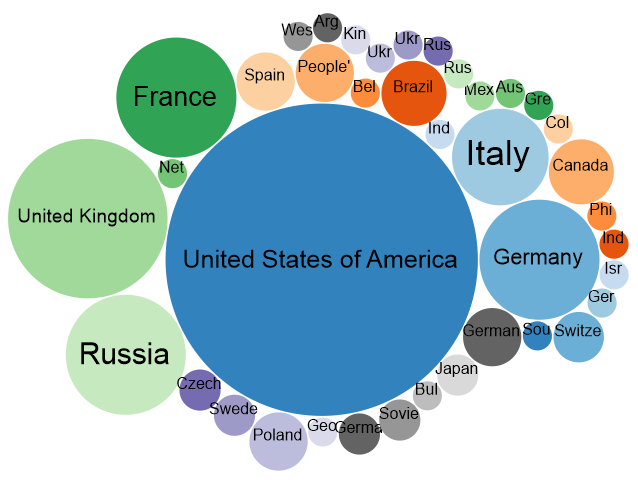
\includegraphics[width=0.95\textwidth]{./chapter/aircraft/Manufacture-with-country_en_2017.png}
	\caption{The ratio of the number of aircraft manufacturers by country, 2017.}
	\label{fig:Manufacture-with-country_en_2017}
\end{figure}

As can be seen from the response to request~\ref{lst:aircraft_listing_7} in Fig.~\ref{fig:Manufacture-with-country_en_2017}, not all existing 
aircraft manufacturers are listed, as evidenced by the data taken from the \href{https://www.aviationfanatic.com/}{aviationfanatic.com}. 
More information about the lack of data in Wikidata is given in the next section of this chapter. 
%Most manufacturers are indicated in the USA (115), Great Britain (30), Germany (17), Russia (17) as of May 2017.

\label{question:aircraft_question_4}
\marginnote{
What is the name of an aircraft held in the air by a huge tank of flammable, lethal gas, located directly above the heads of passengers?
\\
The answer is on page~\pageref{answer:aircraft_question_airship_en}.
}


\begin{figure}[h!]
\centering
	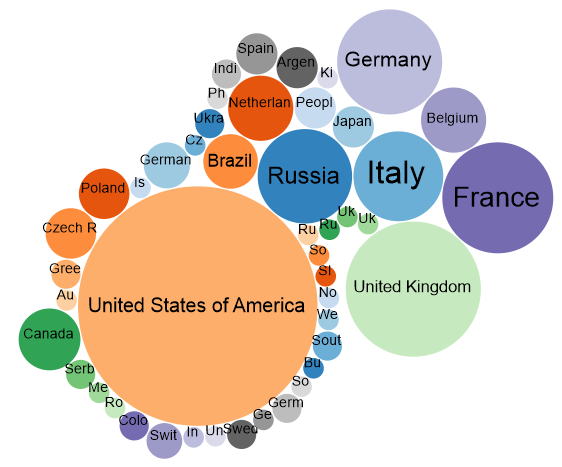
\includegraphics[width=0.95\textwidth]{./chapter/aircraft/Manufacture-with-country_2020_en.png}
	\caption{The ratio of the number of aircraft manufacturers by country, 2020.}
	\label{fig:Manufacture-with-country_2020_en}
\end{figure}


Comparing two bubble charts for 2017 (Fig.~\ref{fig:Manufacture-with-country_en_2017}) and 2020 (Fig.~\ref{fig:Manufacture-with-country_2020_en}), 
we can conclude that the main aircraft manufacturers in the world in 2017 and 2020 were: USA (115 plants in 2017 and 135 plants in 2020), 
Great Britain (30 and 43 plants), Germany (17 and 26 plants) and Russia (17 and 21 plants). The USA is still the leader, but France in 3 years 
managed to outstrip Germany, increasing the number of production facilities to 29 (Germany~--- 26), thus taking the third place. But in general, 
the ratio of aircraft production between different countries remains the same.

%%%%%%%%%%%%%%%%%%%%%%%%%%%%%%%%%%%%%%%%%%%%%%%%%%%%%%%

\section{Completeness of Wikidata}


\label{question:aircraft_question_5}
\marginnote{
Which aircraft is shown in Fig. \ref{fig:airship_question_aircraft_en}?
}


\begin{marginfigure}
{
\setlength{\fboxsep}{0pt}%
\setlength{\fboxrule}{1pt}%
\fcolorbox{gray}{gray}{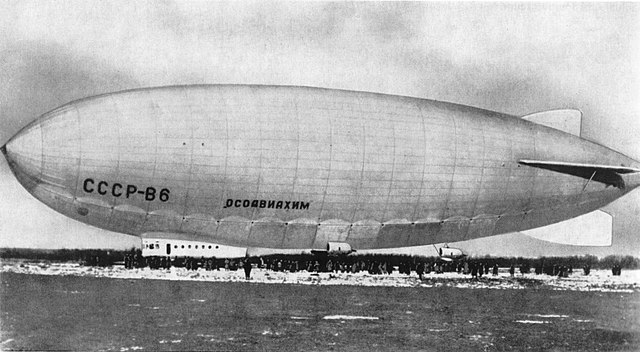
\includegraphics[width=\linewidth]{./chapter/aircraft/foto_of_airship.jpg}}%
}
  \caption{Unknown aircraft.}%
  \label{fig:airship_question_aircraft_en}%
\end{marginfigure}


\marginnote{
The answer is on page~\pageref{answer:aircraft_question_airship_2_en}.
}


Based on the above data, it is possible to predict when Wikidata will include all data from aviationfanatic.com. In three years, 
the number of aircraft manufacturers increased by 239, representing an annual increase of about 80 aircraft manufacturers. 
Also during this time, information on 295 aircraft manufacturers was entered into Wikidata, that is, about a hundred aircraft factories 
are added annually. For 2020, there was no information on Wikidata about the \num{1344} aircraft manufacturers listed 
on \href{https://www.aviationfanatic.com/}{aviationfanatic.com}. Assuming that a fixed number of new aircraft manufacturers are added 
annually and the number of entries in Wikidata remains unchanged, we can assume that in about 75 years (i.e. 2095), Wikidata will contain 
records of all aircraft manufacturers listed on the aviationfanatic website. com.

The category \Wikiref{Category:Aircraft manufacturers of Russia} indicates the presence in Russia of 58 aircraft manufacturing companies 
in 2017 and 62 plants, institutes and corporations related to aircraft manufacturing in 2020, but at the same time on the 
website \href{https://www.aviationfanatic.com/}{Aviationfanatic.com} lists 61 plants in 2017 and 71 in 2020. 
Among the aircraft building companies in Russia are such companies as: \Wikiref{Irkut Corporation}, \Wikiref{MiG}, \Wikiref{Tupolev}.

%%%%%%%%%%%%%%%%%%%%%%%%%%%%%%%%%%%%%%%%%%%%%%%%%%%%%%%

\section{Exercises}
 
\begin{enumerate}
\item Find the plane with the maximum flight radius.
\item Mark on the political map of the world the location of the main offices of aircraft manufacturers.
\item Find the manufacturer with the maximum number of aircraft manufactured using the \href{https://w.wiki/vF7}{\textit{manufacturer (P176)}} property for aircraft.
\item When was the first aircraft built?
\item Which firms were the first to produce 10, 100 and a thousand aircraft?
\item Draw a chart of the number of aircraft produced in the world and in Russia by year.
\end{enumerate}

\setchapterimage[6cm]{chapter/anime/Kiki.png}

\chapter{Anime: the mysterious and stunning world of Japanese animation\protect\footnotemark}

\labch{anime}

\footnotetext{Background image: \href{https://en.wikipedia.org/wiki/Krita\#Mascot}{Kiki}, the anime-styled \href{https://en.wikipedia.org/wiki/Mascot}{mascot} of Krita, a free graphics editor. 
DeviantArt / \href{https://www.deviantart.com/tysontan/art/The-Magic-Stylus-570566846}{Tyson Tan} (CC BY-SA).}

\marginnote[0.0cm]{Seiyu are Japanese voice actors. Typically they give voice to the characters of anime series and movies as well as video games, and do other narrative work for radio and TV productions. In addition, seiyu do advertisements, announcements, textbook recordings and voiceovers. Both adults and children work as seiyu.}

This chapter is dedicated to \wdqName{anime}{1107} Wikidata object analysis. Using SPARQL queries executed on Wikidata objects of anime type, several tasks were accomplished. These include a list of seiyu (voice actors) and their number of roles, a line chart of seiyu who have acted in one or more anime, a directed graph connecting seiyu and anime they voiced and estimates of the ages of seiyu at the time(s) of voice work.

\section{Anime objects}

\begin{marginfigure}[0.0cm]
{
	\setlength{\fboxsep}{0pt}%
	\setlength{\fboxrule}{1pt}%
	\fcolorbox{gray}{gray}{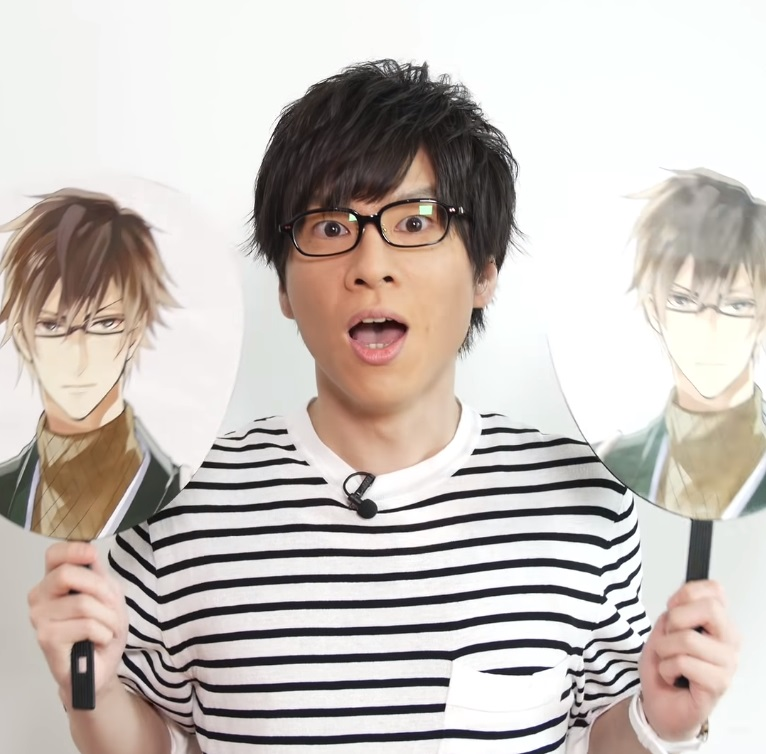
\includegraphics{chapter/anime/seyu.jpg}}
}
\caption
[Seiyu Kenji Akabane, 2021.]
{
Seiyu Kenji Akabane voiced the character Sasuke Sarutobi in the video game \emph{Ikemen Sengoku}, 2018.\newline
Wikimedia Commons / numan (CC BY-SA)
}
\label{fig:seiyu}
\end{marginfigure}

Anime is Japanese animation. It has its own marked visual style, but there are other features that are not so obvious. For instance, anime has a significantly wider variety of genres in comparison to American and European animation~--- from family and kids' comedies to dramas, the latter of which are usually depicted with live actors in Western cinema.

Each anime has its own voice actors. From here on we will refer to the Japanese voice actors as \emph{seiyu}. In Japanese animation the terms \emph{seiyu} and \emph{voice actor} are synonymous. The designation \emph{title} will usually reference certain anime and associated manga (Japanese comics). In general, \emph{title} is a term that includes various media products, from novels to films, that are of the same name and are based on one or the other.

In order to work with the anime list from Wikidata we need to use the \wdqName{anime}{1107} object and the \wdProperty{31}{instance of} property. Let us retrieve the list of all anime titles, without taking the subclasses into account, with query~\ref{lst:anime}.

\begin{lstlisting}[ language=SPARQL, breaklines=true, numbers=none,%
                    caption={List of anime without subclasses. The result contained \num{683} instances of anime in 2017 and \num{216} in 2021. SPARQL query: \href{https://w.wiki/4ABq}{w.wiki/4ABq}},%
                    label=lst:anime,%
                    texcl%
                    ]
# List of instances of anime
SELECT ?anime ?animeLabel WHERE {
    ?anime wdt:P31 wd:Q1107. # instance of anime
    SERVICE wikibase:label{bd:serviceParam
					     wikibase:language "en,ja"}
}
\end{lstlisting}%

There are many more anime objects in Wikidata, but they are not instances of anime but of its subclasses, for example, \wdqName{anime series}{63952888}. Let us execute the query~\ref{lst:anime_genres} in order to obtain the list of anime genres and the number of anime that correspond to these genres.

% full width lstlisting, format=llapwide18 (-1.8cm), see kao.sty
\begin{widepar}%
	\captionsetup[lstlisting]{%
        format=llapwide18 % llap - at margin, margin - at main text
		%indention=0pt,parindent=0pt,belowskip=0pt,aboveskip=0pt%
	}%
\begin{lstlisting}[ language=SPARQL, breaklines=true, numbers=none,%
                    %captionpos=t,belowcaptionskip=25pt,abovecaptionskip=25pt,%
                    caption={List of genres (subclasses) of anime. The result contained 11 genres of anime in 2021. SPARQL query: \href{https://w.wiki/4ABt}{w.wiki/4ABt}},%
                    label=lst:anime_genres,%
                    texcl%
                    ]
# Select anime and its subclasses with number of titles corresponding to these subclasses
SELECT ?subAnime ?subAnimeLabel (COUNT(?subAnimeInstance) AS ?count) WHERE {
  ?subAnime wdt:P279* wd:Q1107.
  ?subAnimeInstance wdt:P31 ?subAnime.
  SERVICE wikibase:label {bd:serviceParam wikibase:language "en,ja"}
}
GROUP BY ?subAnime ?subAnimeLabel
ORDER BY DESC(?count)
\end{lstlisting}%
\end{widepar}%

%\vspace{-0.5cm}
In Fig.~\ref{fig:anime_piechart}, the distribution of anime to genres is visualized with a sunburst diagram.

This classification of anime by genre is not perfect because it is significantly skewed toward anime television series: among the \num{4875} anime titles, \num{2984} are instances of the anime series genre (\num{62.7}\%). Also, some subclasses correspond not to genres, but to particular anime (e.g., \href{https://w.wiki/3iKe}{\emph{Evangelion}}).

Let us retrieve the list of all anime titles that are instances of anime subclasses by using query~\ref{lst:all_anime_list}.

\begin{lstlisting}[ language=SPARQL, breaklines=true, numbers=none,
                    caption={List of anime with titles that are instances of anime subclasses.
                        The result contained \num{4875} anime titles in 2021.
                        SPARQL query: \href{https://w.wiki/4ABv}{https://w.wiki/4ABv}
                        },
                    label=lst:all_anime_list,
                    texcl 
                    ]
# List of instances of anime and subclasses of anime
SELECT ?anime ?animeLabel
WHERE
{
  ?anime wdt:P31/wdt:P279* wd:Q1107.  # instance of anime
                                      # with subclasses
  SERVICE wikibase:label{ bd:serviceParam 
                          wikibase:language "en,ja" }
}
\end{lstlisting}%

\begin{marginfigure}[0.0cm]
{
	\setlength{\fboxsep}{0pt}%
	\setlength{\fboxrule}{1pt}%
	\fcolorbox{gray}{gray}{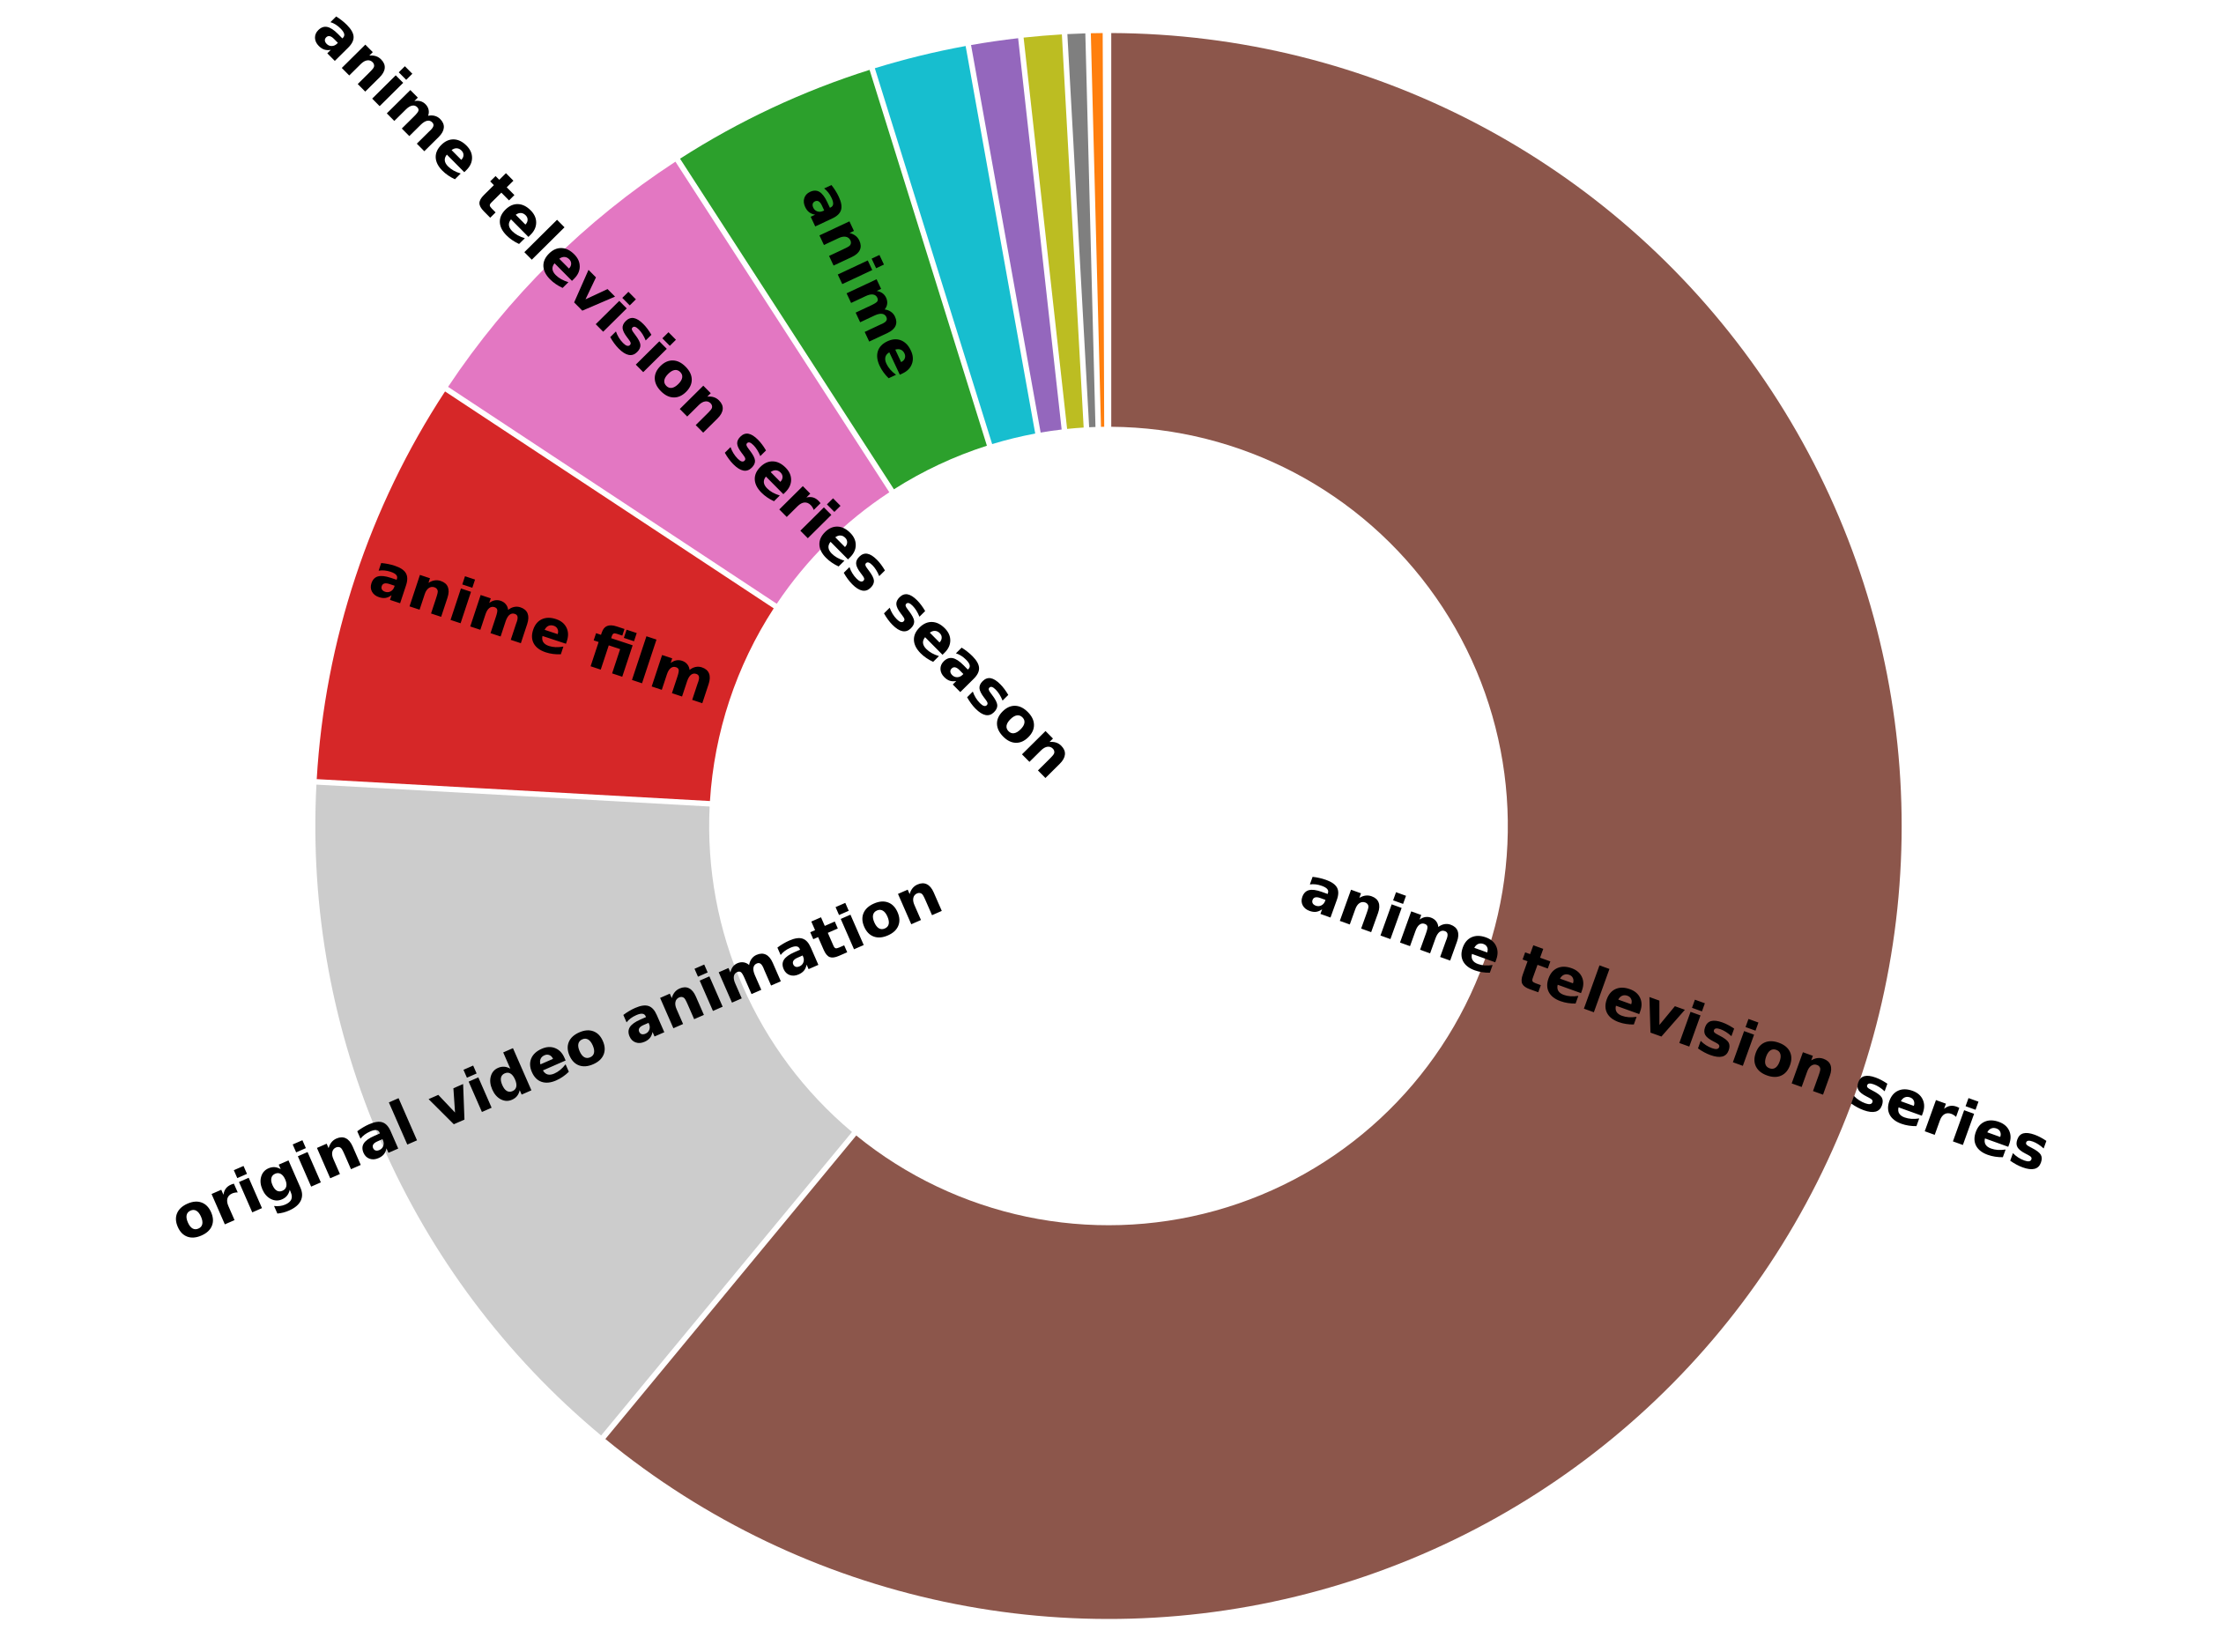
\includegraphics[scale=1.5]{chapter/anime/anime-genres-sunburst-en-2021.png}}
}
\caption
[Anime genres on sunburst diagram, 2021.]
{
Sunburst diagram of anime genres\index{Chart!Sunburst diagram!Nuber of anime per genre} created with Rawgraphs\index{Data analysis services!Data visualization services!Rawgraphs} (\href{https://app.rawgraphs.io}{https://app.rawgraphs.io}).\newline
}
\label{fig:anime_piechart}
\end{marginfigure}

Anime that have the most complete information on Wikidata are \wdqName{Gurren Lagann}{4277}, \wdqName{Space Battleship Yamato}{4292} and \wdqName{Project A-ko}{4316}. There are also some anime with many missing properties, including \wdqName{Doraemon}{711311}, \wdqName{The Animal Conference on the Environment}{97195557} and \wdqName{Assassins Pride}{96737300}.

According to a profiling of Wikidata using ProWD \autocite{anime_prowd}, among all the anime titles, \wdqName{Fullmetal Alchemist: The Sacred Star of Milos}{1004318}\footnote{\emph{Fullmetal Alchemist: The Sacred Star of Milos} is an anime movie that continues the \emph{Fullmetal Alchemist} series. Its main characters are two alchemist brothers who use their magic to fight criminals and the forces of evil.} has the greatest number of properties (\num{24}).

\section{List of seiyu ordered by their number of roles in anime}

Naturally, there are multiple characters in anime. Accordingly, different seiyu give voice to them. Most seiyu have taken part in a number of anime, but some have even managed to work on several dozen titles. Talented seiyu are sometimes invited to voice different characters in one anime. \href{https://w.wiki/4UFa}{Hiroshi Kamiya} is one of the most popular seiyu. He has worked on more than 180 anime and earned many awards. \href{https://w.wiki/4UFh}{\emph{Attack on Titan}} is one of the most famous anime with his participation in which he voiced Captain Levi, one of the main characters.

Let us create a list of seiyu ordered according to the number of anime voiced by them (query~\ref{lst:seiyu_titles_sorted}).

\begin{lstlisting}[ language=SPARQL, breaklines=true, numbers=none,
                    caption={Sorted list of seiyu according to the number of anime voiced by them.
                        \num{148} results in 2017, and \num{2910} in 2021.
                        SPARQL query: \href{https://w.wiki/4Xos}{https://w.wiki/4Xos}
                        },
                    label=lst:seiyu_titles_sorted,
                    texcl 
                    ]
# Ordered list of actors (seiyu) according to the number
# of anime where they took part in.
SELECT ?seiyu ?seiyuLabel (COUNT(?anime) AS ?count)
WHERE
{
  ?anime wdt:P31/wdt:P279* wd:Q1107;  # anime/subclass
         wdt:P725 ?seiyu.  # instance of seiyu
  SERVICE wikibase:label { bd:serviceParam wikibase:language "en,ja" }
}
GROUP BY ?seiyu  ?seiyuLabel  # group by seiyu 
ORDER BY DESC(?count)  # order by count of voiced anime
\end{lstlisting}%

\section{Chart of number of seiyu who worked on one or more anime}

We can create a line chart with seiyu plotted according to their total number of roles. The more anime seiyu have voiced, the farther to the right they are on the diagram. We can use query~\ref{lst:seiyu_titles_graph} to create the chart.

\begin{lstlisting}[ language=SPARQL, breaklines=true,
                    caption={Line chart with the number of seiyu along the Y-axis and the number anime voiced by them along the X-axis.
                        \num{13} results in 2017, \num{58} results in 2021.
                        SPARQL query: \href{https://w.wiki/4UX8}{https://w.wiki/4UX8}
                        },
                    label=lst:seiyu_titles_graph,
                    texcl 
                    ]
# Graph of the number of voice actings of different seiyu
#defaultView:LineChart
SELECT ?seiyuRoles (COUNT(?seiyuRoles) AS ?quantity) WHERE {
  FILTER(?seiyuRoles < 71)
  {
     SELECT (COUNT(?seiyu) AS ?seiyuRoles) WHERE {
       ?anime wdt:P31/wdt:P279* wd:Q1107;
              wdt:P725 ?seiyu.
       SERVICE wikibase:label { bd:serviceParam wikibase:language "en,ja"}
     }
     GROUP BY ?anime
     ORDER BY DESC(?seiyuRoles)
  }
}
GROUP BY ?seiyuRoles
ORDER BY DESC(?seiyuRoles)
}
\end{lstlisting}%

Figure~\ref{fig:Seiyu_num_chart_2021_en} shows that the higher the number of voiced anime is, the lower the number of seiyu who attain so many roles. Line \num{4} of query~\ref{lst:seiyu_titles_graph} sets the limit at \num{71} anime as there are only a few seiyu who have worked on a larger number of anime, and expanding the graph farther to the right would not be informative.

As Figure~\ref{fig:Seiyu_num_chart_2021_en} shows, most seiyu have voiced only one anime during their life. On the chart, there are \num{254} such seiyu. However, seiyu is a profession to which people often devote their lives. The fact that many voiced only one role in their lives according to Wikidata seems to be a result of the incompleteness of the data set.

\index{Chart!LineChart!Number of seiyu who voiced one or more anime}
\begin{figure*}[h]

    \setlength{\fboxsep}{0pt}%
    \setlength{\fboxrule}{1pt}%
    \fcolorbox{gray}{gray}{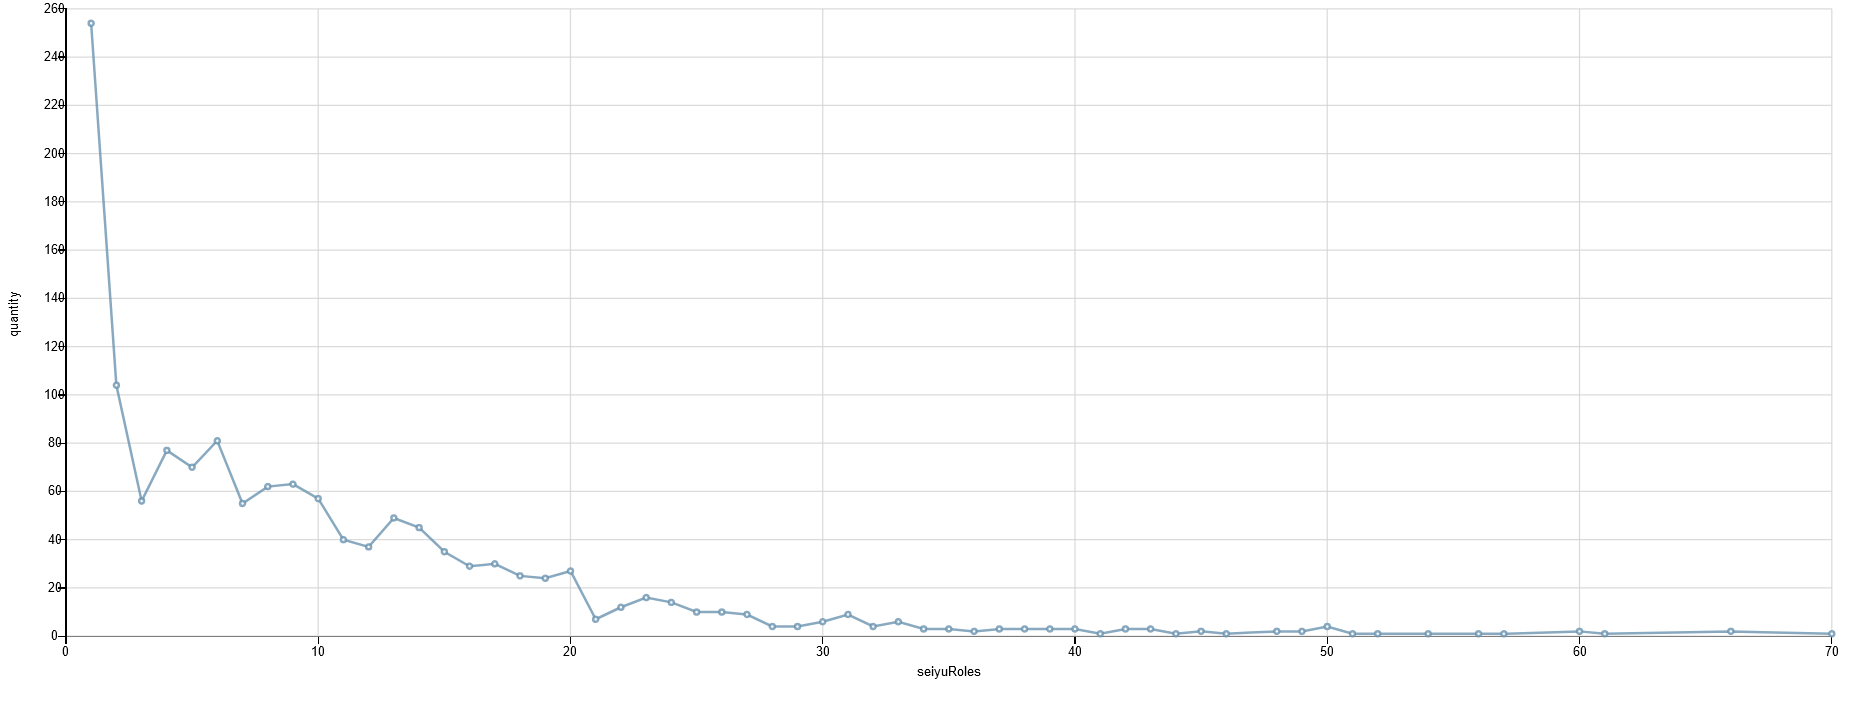
\includegraphics[width=\linewidth]{chapter/anime/Seiyu_chart_2021_en.png}}
	\caption[Chart of the number of roles voiced by different seiyu, 2021.]{Chart of number of roles voiced by different seiyu, 2021. The chart is constructed using the output of query~\ref{lst:seiyu_titles_graph}.}%
    \label{fig:Seiyu_num_chart_2021_en}%
\end{figure*} 

\section{Graph that connects seiyu to anime they have voiced}

Most of the seiyu give voice to multiple characters from different anime. Let us create a graph that connects seiyu to anime they have voiced (query ~\ref{lst:seiyu_graph}).

Figure~\ref{fig:Seiyu_graph_en} shows part of the graph for several famous seiyu.

% full width lstlisting, format=llapwide18 (-1.8cm), see kao.sty
\begin{widepar}%
\captionsetup[lstlisting]{format=llapwide18}%
%
\begin{lstlisting}[ language=SPARQL, breaklines=true,%
                    caption={Graph that connects seiyu to anime they have voiced. \num{826} results in 2017, and \num{496} in 2021. SPARQL query: \href{https://w.wiki/4Xqk}{https://w.wiki/4Xqk}},
                    label=lst:seiyu_graph,
                    texcl
                  ]
# Graph of seiyu and anime they took part in
#defaultView:Graph
SELECT DISTINCT ?item ?itemLabel ?rgb ?link
WHERE
{ # voice actors (seiyu) with more than one anime
  VALUES ?toggle { true false }
  VALUES ?seiyu { wd:Q1207010 wd:Q233902 wd:Q1323728 }
  ?anime  wdt:P31/wdt:P279* wd:Q1107; # instance of anime or its subclass
          wdt:P725 ?seiyu;            # seiyu who voiced this anime 
  SERVICE wikibase:label {bd:serviceParam wikibase:language "en,ja"}
  BIND(IF(?toggle,?anime,?seiyu) AS ?item).
  BIND(IF(?toggle,?animeLabel,?seiyuLabel) AS ?itemLabel).
  BIND(IF(?toggle,"FFFFFF","7FFF00") AS ?rgb).
  BIND(IF(?toggle,"",?anime) AS ?link).
}
\end{lstlisting}%
\end{widepar}%

The \emph{?seiyu} variable (line 7) contains an array of Wikidata objects that correspond to several seiyu including \wdqName{Bin Shimada}{1323728} and others. We picked only three seiyu for illustrative purposes as a graph including more seiyu would be unwieldy for reading.

The \emph{BIND\index{SPARQL!BIND!Graph that connects seiyu to anime they have voiced}(IF\index{SPARQL!IF!Graph that connects seiyu to anime they have voiced}(?toggle, ?anime, ?seiyu))} construction in line \num{11} determines the graph node type: if \emph{?toggle} is \emph{true}, then the node corresponds to anime, and seiyu otherwise. The item label and the node color are determined in the same way in lines \num{12} and \num{13}. Line \num{14} creates the edges linking the seiyu and anime nodes.

\index{Chart!Graph!Part of graph that connects seiyu to anime they have voiced}
\begin{figure*}

    \setlength{\fboxsep}{0pt}%
    \setlength{\fboxrule}{1pt}%
    \fcolorbox{gray}{gray}{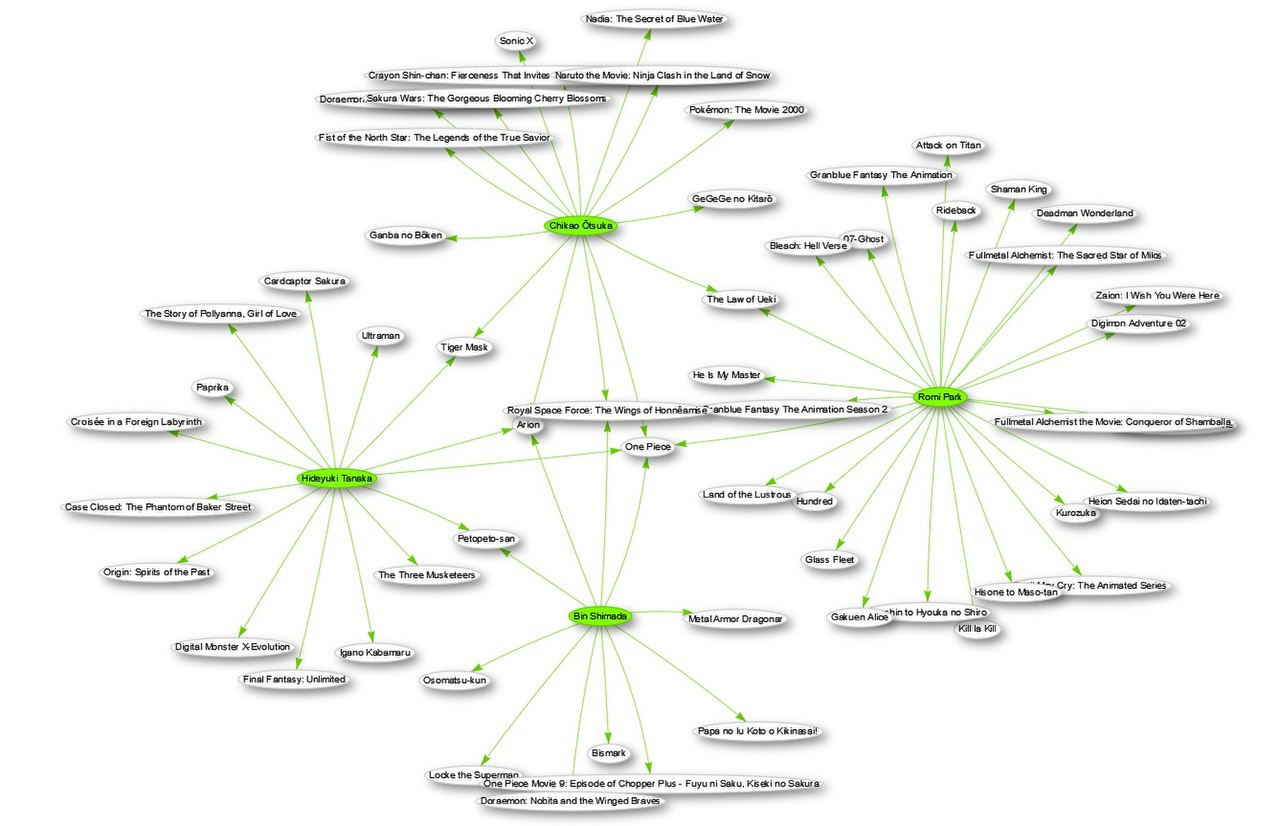
\includegraphics[width=\linewidth]{chapter/anime/Seiyu_graph_en_sm.jpg}}
	\caption[Part of graph that connects seiyu to anime they have voiced, 2021.]{Part of graph that connects seiyu and the anime they took part in, 2021. The graph is constructed using the output of query~\ref{lst:seiyu_graph}.}%
    \label{fig:Seiyu_graph_en}%
\end{figure*} 

\section{Fullness of Wikidata}

The list of anime of \href{https://w.wiki/4Xs4}{English Wikipedia} contains around \num{1600} titles. But there are special websites dedicated to anime, such as \href{https://www1.gogoanime.cm/}{Gogoanime online cinema}\sidenote{Gogoanime | Watch anime online, English anime online HD. \href{https://www1.gogoanime.cm/}{https://www1.gogoanime.cm/}, 2021} which contain information about many more titles. At the time of writing, there were \num{10072} anime on Gogoanime (\num{74} pages of \num{136} titles each plus one page of \num{8}), whereas Wikidata provides information for only about \num{4875} titles (see query~\ref{lst:all_anime_list}). In addition, we should take into account the rapidness of anime releases\sidenote{Exercise: Using SPARQL, count the number of anime released in the preceding year.}. As such, we can conclude that Wikidata does not reflect accurate information about anime (only \num{48.4}\% of titles are represented).

We cannot consider Gogoanime a \href{https://w.wiki/Eiw}{reliable source (RS)}\sidenote{RS: a reliable source, according to Wikipedia, is a source of information that is first and foremost unbiased and verifiable. See \href{https://w.wiki/Eiw}{https://w.wiki/Eiw}}, but it can be used to analyze the incompleteness of Wikidata.

Let us recall Query~\protect\ref{lst:seiyu_titles_sorted}, which returned \num{2910} names of seiyu from Wikidata. The problem is that we searched only for voice actors who have worked on anime. When we query the names of all voice actors, without the anime restriction, the resulting number increases by a factor of five (see Query~\protect\ref{lst:voice_actors_list}). Such an increase tells us that seiyu do not only voice anime, and we should consider this fact in  future.

\begin{lstlisting}[ language=SPARQL, breaklines=true, numbers=none,
                    caption={Creates ordered list of actors according to the number of projects voiced by them.
                        \num{3965} results in 2017, \num{14742} results in 2021.
                        SPARQL query: \href{https://w.wiki/4XpD}{https://w.wiki/4XpD}
                        },
                    label=lst:voice_actors_list,
                    texcl 
                    ]
# Ordered list of actors according to the quantity
# of projects voiced by them
SELECT ?actor ?actorLabel (COUNT(?anime) AS ?count)
WHERE
{
  ?anime wdt:P725 ?actor.	 # instance of voice actor
  SERVICE wikibase:label{ bd:serviceParam
			  								wikibase:language "en,ja" }
}
GROUP BY ?actor	?actorLabel
ORDER BY DESC(?count)	# order by number of voiced projects
\end{lstlisting}%

\index{Chart!Sunburst diagram!Number of roles voiced by different actors}
\begin{figure*}

    \setlength{\fboxsep}{0pt}%
    \setlength{\fboxrule}{1pt}%
    \fcolorbox{gray}{gray}{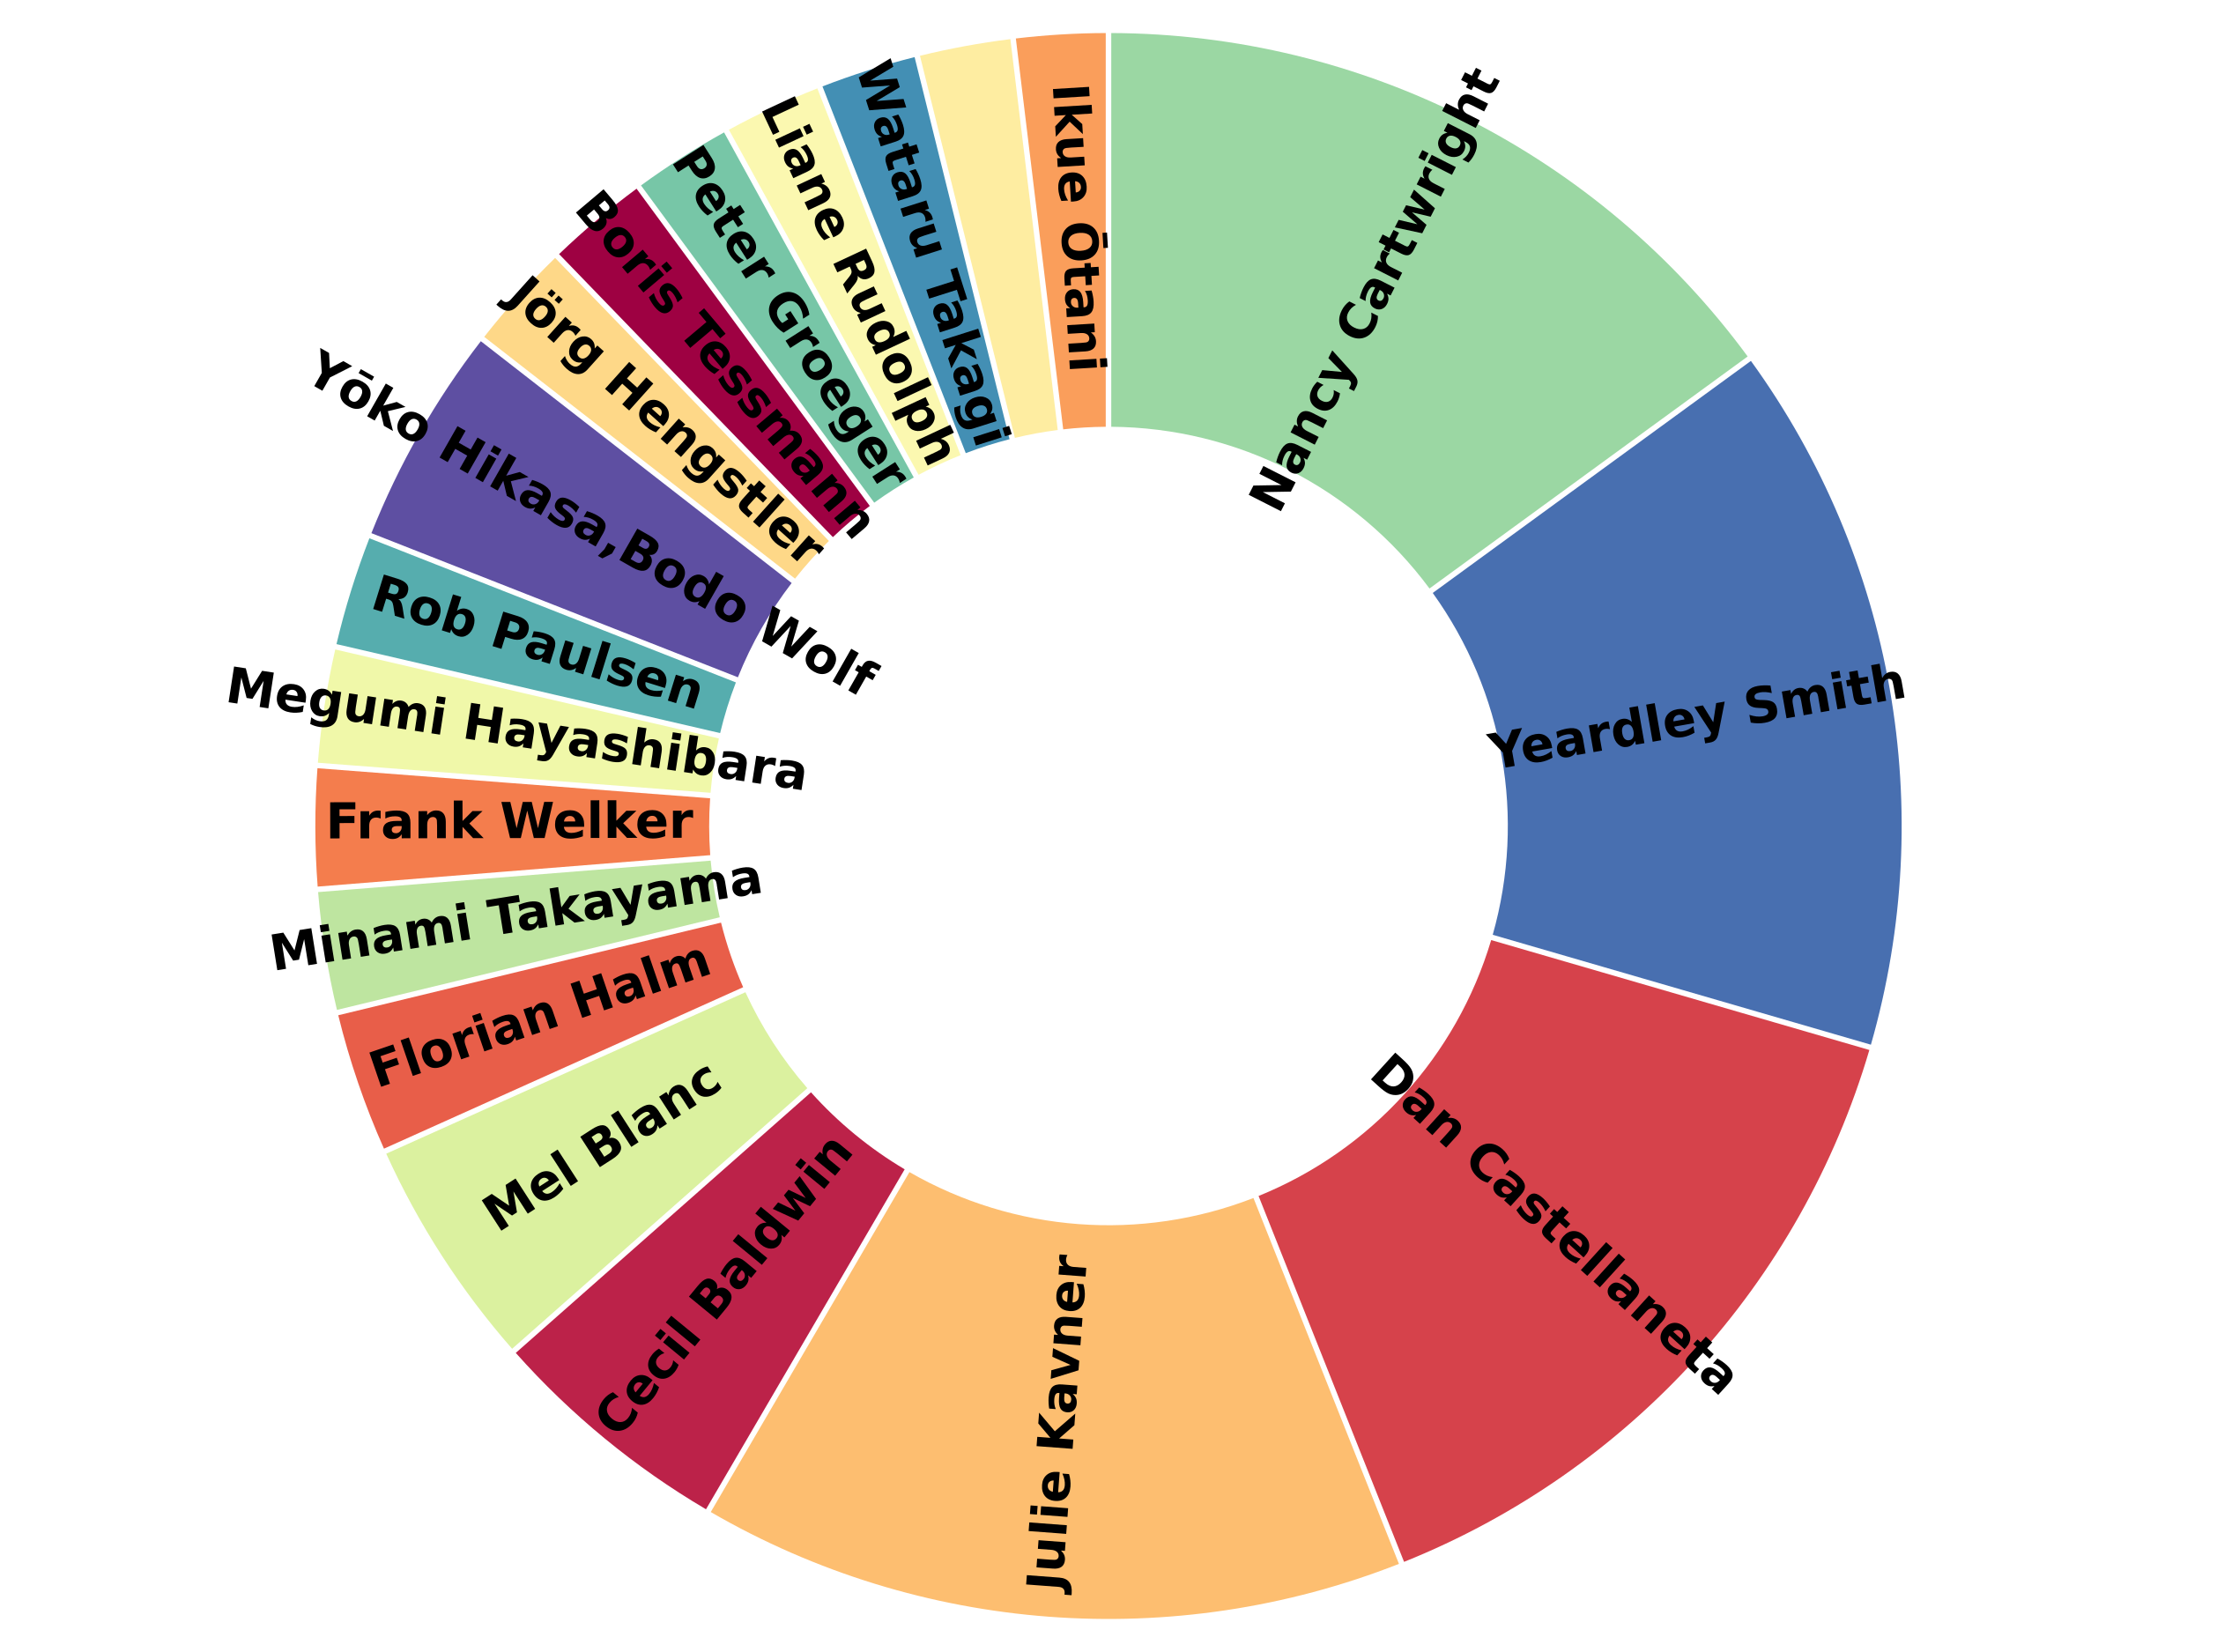
\includegraphics[width=\linewidth]{chapter/anime/actors-rawgraphs-2021-en.png}}
	\caption[Sunburst diagram of number of roles voiced by different actors, 2021.]{Sunburst diagram of number of roles voiced by different actors, 2021. The diagram is constructed using the output of Query~\ref{lst:voice_actors_list} in \href{https:\\app.rawgraphs.io}{Rawgraphs\index{Data analysis services!Data visualization services!Rawgraphs}}.}%
    \label{fig:Actors_sunburst_en}%
\end{figure*}

The sunburst diagram, Figure.~\ref{fig:Actors_sunburst_en}, is one way to visualize the output of Query~\ref{lst:voice_actors_list}. Such a diagram allows us to see the actors who contributed the most to the voice acting industry.

\section{Is the release date of anime available?}

Fans of anime often want to know the release date of their favorite titles. Wikidata does not always contain complete information on release dates. Let us retrieve the number of anime of which the release date is not available using Query~\ref{lst:anime_no_pub_date}.

\begin{lstlisting}[ language=SPARQL, breaklines=true, numbers=none,
                    caption={Retrieves list of anime of which the release date is not specified.
                        \num{237} results in 2017, and \num{2940} in 2021.
                        SPARQL query: \href{https://w.wiki/4ACU}{https://w.wiki/4ACU}
                        },
                    label=lst:anime_no_pub_date,
                    texcl 
                    ]
# List of anime the release date of which
# is empty
SELECT ?anime ?animeLabel
WHERE
{
    ?anime wdt:P31/wdt:P279* wd:Q1107;  # instance of anime
    FILTER NOT EXISTS { ?anime wdt:P577 [] } # no release date
    SERVICE wikibase:label{ bd:serviceParam
			  									wikibase:language "en,ja" }
}
\end{lstlisting}%

Release dates of \num{2940} anime out of \num{4875} titles on Wikidata are not specified, or \num{60.3}\%. In 2017, \num{237} of \num{683} titles (\num{34.7}\%) did not have a release date.It seems, unfortunately, an increase in the number of values for a list is not always accompanied by quality property information\sidenote{Exercise: Write a query to calculate the proportion of anime that do not have a specified release date, relative to all anime on Wikidata. Compare this proportion with the proportion for 2021 (\num{60.3}\%) and make a conclusion about the change of the quality of Wikidata.}.

\section{Anaysis of age when seiyu perform voice acting}

As for any other profession, voice actors have age when they dub multiple anime. Usage of SPARQL and external data mining tools like Python\index{Programming languages!Examples of programming languages!Python} programming language\sidenote{Python is an interpretable programming language that is used for different purposes due to its flexibility. For example, it can be used to work with Wikidata: chapter~\ref{ch:bots} (page~\pageref{ch:bots}) describes the process of creation of bots for Wikidata.} allows to estimate such an age according to Wikidata.

In order to obtain the input data for our study, we need to execute three SPARQL scripts and export their output to .csv\sidenote{CSV (comma-separated values) is a format of tabular data that stores the table as a sequence of text lines. These lines contain the values of table columns splitted by comma.} files. Next, these CSV files are used in Python script which generates the output chart. You can run Python programs on Google Colaboratory\sidenote{Google Colaboratory (Colab) is a cloud code editor which allows to write and execute Python scripts and share them with other people. In addition, Colab provides processors and graphic cards that allow to run complex algorithms such as neural networks. Colab is available at \href{https://colab.research.google.com}{https://colab.research.google.com}.}.

We can get the listis of all seiyu and their birth dates on Wikidata in two ways (scripts~\ref{lst:seiyu_bd_w_service} and~\ref{lst:seiyu_bd_w_rdfs}): using \emph{SERVICE} command and \emph{rdfs:label} construction.

The difference between the scripts is that:

\begin{itemize}
    \item{the label (name) of seiyu is retrieved with the \emph{?seiyuLabel} variable in the first script (the \emph{SERVICE}\index{SPARQL!SERVICE!Retrieval of seiyu birth dates} command that defines the languages of output should be used in this case) and with the \emph{rdfs:label} command in the second script;}
    \item{in the first script, the \emph{?seiyuLabel} variable has to be passed as a parameter to \emph{GROUP BY}\index{SPARQL!GROUP BY!Retrieval of seiyu birth dates} in order to connect seiyu objects and their labels.}
\end{itemize}

\begin{lstlisting}[ language=SPARQL, breaklines=true, numbers=none,
                    caption={Get seiyu and their birth dates with SERVICE command.
                        \num{2515} results in 2021.
                        SPARQL query: \href{https://w.wiki/4Ftb}{https://w.wiki/4Ftb}
                        },
                    label=lst:seiyu_bd_w_service,
                    texcl 
                    ]
# Get list of all seiyu objects, their names
# and birth dates
SELECT ?seiyu ?seiyuLabel ?bDate
WHERE {
  ?anime (wdt:P31/(wdt:P279*)) wd:Q1107;
    wdt:P725 ?seiyu.       # seiyu is anime voice actor
  ?seiyu wdt:P569 ?bDate.  # has a birthday
  SERVICE wikibase:label
						{bd:serviceParam wikibase:language "en,ja"}
}
GROUP BY ?seiyu ?seiyuLabel ?bDate
}
\end{lstlisting}%

\begin{lstlisting}[ language=SPARQL, breaklines=true, numbers=none,
                    caption={Get seiyu and their birth dates with rdfs:label.
                        \num{2515} results in 2021.
                        SPARQL query: \href{https://w.wiki/4FPn}{https://w.wiki/4FPn}
                        },
                    label=lst:seiyu_bd_w_rdfs,
                    texcl 
                    ]
# Get list of all seiyu objects, their names
# and birth dates
SELECT ?seiyu (SAMPLE(?seiyu) AS ?seiyuLabel) ?bDate
WHERE {
  ?anime (wdt:P31/(wdt:P279*)) wd:Q1107;
    wdt:P725 ?seiyu.       # seiyu is anime voice actor
  ?seiyu wdt:P569 ?bDate.  # has a birthday 
  ?seiyu rdfs:label ?label.
}
GROUP BY ?seiyu ?bDate
\end{lstlisting}%

Let's get the list of all anime and their release dates on Wikidata with script~\ref{lst:all_anime_releases}\sidenote{Exercise: visualize the output of the script~\ref{lst:all_anime_releases}. To increase the task difficulty, you can add the dates of releases of the series final episodes to the chart.}.

\begin{lstlisting}[ language=SPARQL, breaklines=true, numbers=none,
                    caption={Anime movies and series release dates.
                        \num{5268} results in 2021.
                        SPARQL query: \href{https://w.wiki/4EgY}{https://w.wiki/4EgY}
                        },
                    label=lst:all_anime_releases,
                    texcl 
                    ]
# Get all anime objects, their names and release dates
SELECT ?anime ?animeLabel ?animePubDate
		?animeSeriesStartDate WHERE {
  ?anime (wdt:P31/(wdt:P279*)) wd:Q1107.
  OPTIONAL { ?anime wdt:P577 ?animePubDate. }
  OPTIONAL { ?anime wdt:P580 ?animeSeriesStartDate. }
  SERVICE wikibase:label { bd:serviceParam
					wikibase:language "en,ja" }
}
\end{lstlisting}%

Note that the movies have the \wdProperty{577}{publication dates} property, whereas the series have the \wdProperty{580}{start dates}.

Let's get the links between seiyu and anime dubbed by them (script~\ref{lst:link_anime_seiyu}).

\begin{widepar}
\begin{lstlisting}[ language=SPARQL, breaklines=true,
                    caption={Links between anime and seiyu objects.
                        \num{27092} results in 2021.
                        SPARQL query: \href{https://w.wiki/4ELh}{https://w.wiki/4ELhhttps://w.wiki/4EgY}
                        },
                    label=lst:link_anime_seiyu,
                    texcl 
                    ]
# List of links between seiyu and anime where they are involved in
SELECT DISTINCT ?item ?itemLabel ?link ?itemType
WHERE
{
  VALUES ?toggle { true false }
  ?anime  wdt:P31/wdt:P279* wd:Q1107; # instance of anime or its subclass
          wdt:P725 ?seiyu.            # list seiyu who acted in this anime
  
  BIND(IF(?toggle,?anime,?seiyu) AS ?item).         # connection of "from anime to seiyu" type
  BIND(IF(?toggle,?animeLabel,?seiyuLabel) AS ?itemLabel).  # similar connection between labels
  BIND(IF(?toggle,?seiyu,?anime) AS ?link).            #  connection of "from seiyu to anime" type
  BIND(IF(?toggle,?seiyu,"seiyu") AS ?itemType).    # column to distinguish seiyu and anime items
  # if the item describes a seiyu, its value is "seiyu", the link is kept otherwise
  SERVICE wikibase:label {bd:serviceParam wikibase:language "ru,en,ja"}
}
\end{lstlisting}%
\end{widepar}

The analysis result can be shown as a histogram. To create it, we'll use such Python libraries as \href{https://en.wikipedia.org/wiki/Pandas\_(software)}{Pandas\index{Programming languages!Programming language libraries!Pandas}}\sidenote{Pandas is a Python library that provides multiple useful functions for tabular data processing. \href{https://en.wikipedia.org/wiki/Pandas\_(software)}{https://en.wikipedia.org/wiki/Pandas\_(software), 2021}.} and \href{https://en.wikipedia.org/wiki/Matplotlib}{Matplotlib\index{Programming languages!Programming language libraries!Matplotlib}}\sidenote{Matplotlib Python library allows to plot charts of various types. \href{https://en.wikipedia.org/wiki/Matplotlib}{https://en.wikipedia.org/wiki/Matplotlib, 2021}.}. The script which generates the final historgam is published on \href{https://git.io/J1UGA}{GitHub} service\sidenote{Script is published in the wd\_book project on GitHub: \href{https://git.io/J1UGA}{https://git.io/J1UGA}}.

The histogram has age in years along its X-axis and the total number of roles dubbed by the seiyu of this age along Y-axis. The histogram is present on Fig.~\ref{fig:Seiyu_age_hist_EN}.

\index{Chart!Histogram!Number of anime voiced by seiyu of different ages}
\begin{figure*}[h]

    \setlength{\fboxsep}{0pt}%
    \setlength{\fboxrule}{1pt}%
    \fcolorbox{gray}{gray}{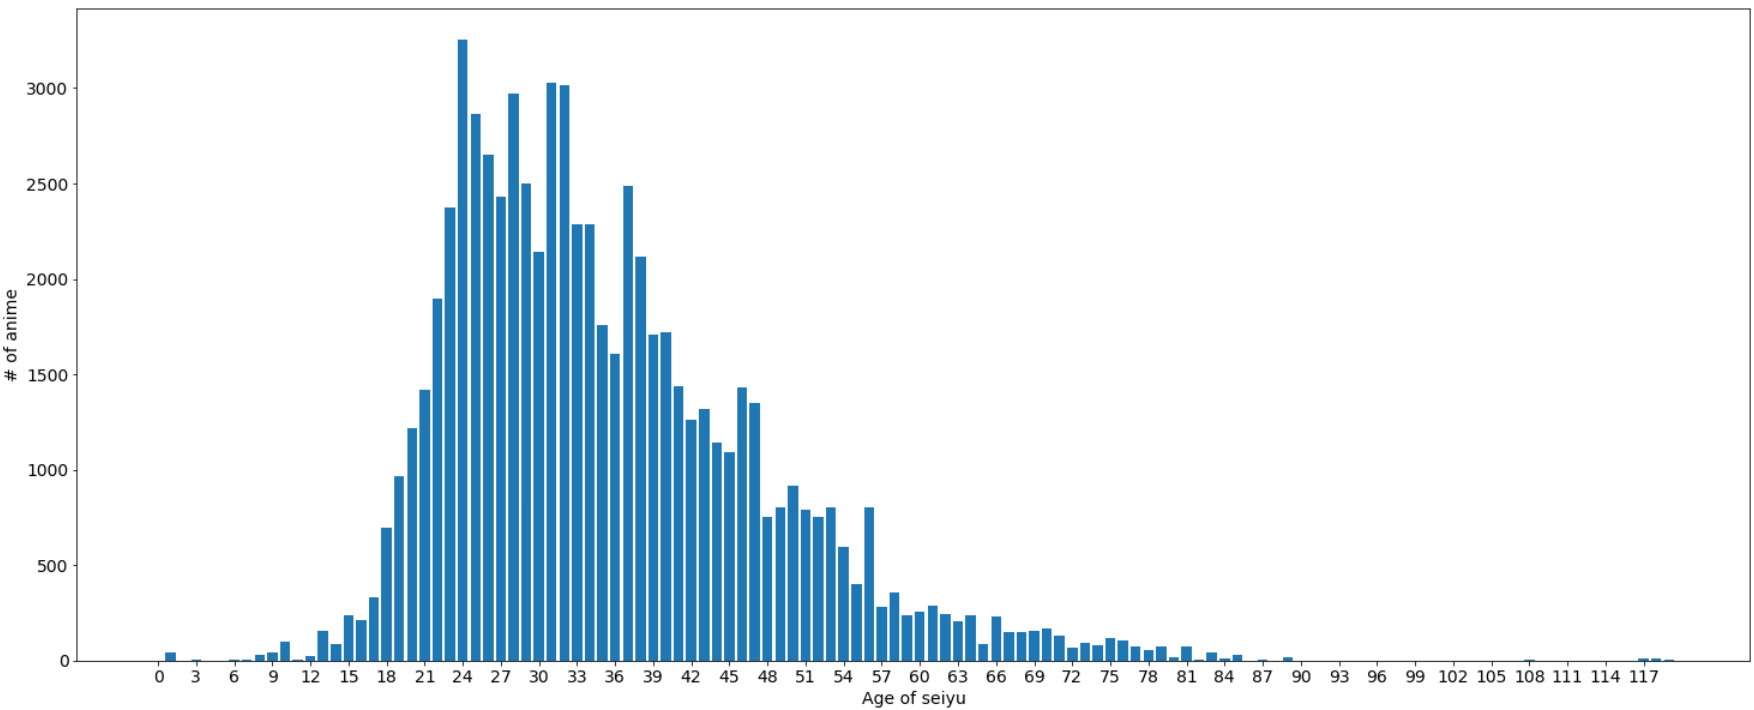
\includegraphics[width=\linewidth]{./chapter/anime/Seiyu_age_hist_EN.png}}
	\caption[Histogram of number of anime voiced by seiyu of different ages, 2021.]{Histogram of number of anime voiced by seiyu of different ages, 2021. The histogram is created according to the output of scripts~\protect\ref{lst:seiyu_bd_w_service} (or~\protect\ref{lst:seiyu_bd_w_rdfs}), \protect\ref{lst:all_anime_releases} and \protect\ref{lst:link_anime_seiyu}.}%
    \label{fig:Seiyu_age_hist_EN}%
\end{figure*} 

There is a fun fact that there are occasions on Wikidata when the seiyu wass born later than the anime with his participation was released. This issue is probably related to absence of the information about the new seasons of re-starts of the anime on Wikidata. For example, in 2021 such a situation happens with the \wdqName{Sazae-san}{11304591} anime and the seiyu named \wdqName{Nobunaga Shimazaki}{5968283}. The seiyu was born in 1988, whereas the anime was published in 1969.

\section{Future work}

\begin{enumerate}
	\item Display the 10 most popular anime released in the current year. Anime popularity is estimated by the number of articles in different language sections. For example, if an article about anime is present in English, Russian and Spanish Wikipedia, then its popularity is equal to three.
	\item Find 5 anime in which the largest number of women seiyu are involved.
	\item Create a bubble chart of the distribution of anime by genre (how many anime are in each genre) using the \wdProperty{279}{subclass} property.
	\item Mark the voice actors' places of birth on the map.
	\item Create a histogram or bubble chart of voice actor nationalities.
	\item Create a histogram of the number of released anime by year or the number of voice actors by year of birth.
	\item Create histograms similar to the figure~\ref{fig:Seiyu_age_hist_EN}, but taking into account the gender of the voice actor (one for men, the other for women).
\end{enumerate}
\setchapterpreamble[u]{\margintoc}
\chapter{Chapter's title}
\labch{the-label-of-your-title2}

\section{The section title}


\chapter[Анализ стран: возраст, формы правления и этнохоронимы]{Анализ трёх аспектов современных стран по Викиданным: возраст стран, популярные формы правления и этнохоронимы}
\label{ch:country}

Эта глава посвящена исследованию стран на основе базы знаний международного проекта Викиданные. С помощью SPARQL-запросов, вычисляемых на объектах <<страна>> в Викиданных, получены: список всех ныне существующих стран, перечень стран, упорядоченных по дате создания, список этнохоронимов стран, пузырьковая диаграмма с формами правления стран, граф соседних стран и карту соседних стран России. Кроме того, проанализирована полнота Викиданных по данной теме.
%%%%%%%%%%%%%%%%%%%%%%%%%%%%%%%%%%%%%%%%%%%%%%%%%%%%%%%

\begin{marginfigure}[0.0cm]
	{
		\setlength{\fboxsep}{0pt}%
		\setlength{\fboxrule}{1pt}%
		\fcolorbox{gray}{gray}{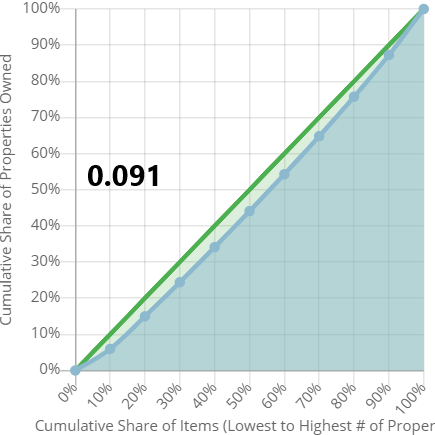
\includegraphics{chapter/country/ProWD_country.png}}
	}
	\caption{
		Высокая степень заполнения по числу свойств объекта Викиданных \href{https://www.wikidata.org/wiki/Q6256}{Страна (Q6256)}.  Данные получены с помощью сервиса \href{https://prowd.id/dashboards/86b6f91a8131/profile}{ProWD.id}, 2020 год. \emph{Коэффициент Джини равен 0.091.}
	}%
	\label{fig:ProWD_country}%
\end{marginfigure}


\section{Список стран и степень полноты информации ряда стран}

Построим список всех стран на английском и русском языках (листинг ~\ref{lst:country}).

\begin{lstlisting}[ language=SPARQL, 
caption={\href{https://w.wiki/k6L}{Экземпляры объекта <<Страна>>}\protect\footnotemark},
label=lst:country, 
escapebegin=ку,escapeend=ку-ку>
]
#List of countries in English and Russian
SELECT ?country ?label_en ?label_ru
WHERE
{
		?country wdt:P31 wd:Q6256. # country
		?country rdfs:label ?label_en filter (lang(?label_en) = "en").
		?country rdfs:label ?label_ru filter (lang(?label_ru) = "ru").
}
\end{lstlisting}

\footnotetext{Получено 205 стран на 2017 год и 175 стран на 2020 год. Ссылка на SPARQL-запрос: \href{https://w.wiki/k6L}{https://w.wiki/k6L}}

По степени заполненности свойств на Викиданнных можно различать <<полные>> и  <<пустые>> страны. 

Примерами наиболее полных и проработанных стран на Викиданных по данным ProWD\cite{prowd_balakireva} являются: \wdqName{Израиль}{801}, \wdqName{Франция}{142}, \wdqName{Соединённые Штаты Америки}{30}.

Почти пустой и малоинформативной страной по данным ProWD является: \wdqName{Срединная Литва}{523380}.

Лидерами среди стран по количеству свойств в Викиданных, по версии ProWD, являются \wdqName{Израиль}{801} и \wdqName{Франция}{142} (по 127 свойств), наименьшее количество свойств у \wdqName{Демократической Республики Вьетнам}{172640} (24 свойства).

%%%%%%%%%%%%%%%%%%%%%%%%%%%%%%%%%%%%%%%%%%%%%%%%%%%%%%%
\section{Возраст стран}

%%%%%%%%%%%%%%%% Упражнение 2 %%%%%%%%%%%%%%%%
\marginnote{
	Какое количество административных единиц имеют следующие страны:
%	У \href{https://w.wiki/mzN}{Латвии} их 119, у \href{https://w.wiki/mzP}{Таиланда} 77, у \href{https://w.wiki/mzR}{Дании} 5, а у \href{https://w.wiki/myt}{России} 81. О чём идет речь?
	\begin{itemize}
		\item Латвия;
		\item Тайланд;
		\item Дания;
		\item Россия.
	\end{itemize}
	См. ответ~\ref{answer:administrative_territorial} на с.~\pageref{answer:administrative_territorial}.
}

Построим список стран, отсортированных по дате основания страны, то есть первом упоминании о стране (листинг ~\ref{lst:age_of_country}).

\begin{lstlisting}[ language=SPARQL, 
caption={\href{https://w.wiki/rN8}{Даты основания стран}\protect\footnotemark},
label=lst:age_of_country, 
escapebegin=ку,escapeend=ку-ку>
]
#List of `instances of` "countries sorted by inception" 
SELECT ?country ?countryLabel ?inception
WHERE
{
		?country wdt:P31 wd:Q6256. # instance of country
		?country wdt:P571 ?inception. # the first mention	
		SERVICE wikibase:label { bd:serviceParam wikibase:language "ru" }
}
ORDER BY (?inception)
}
\end{lstlisting}

\footnotetext{Получено  112 стран на 2017 год и 199 стран на 2020. Ссылка на SPARQL-запрос: \href{https://w.wiki/rN8}{https://w.wiki/rN8}}

В результате выполнения запроса получен список стран с датами их создания. Например, \wdqName{Абхазия}{23334} --- 1 января 0786, \wdqName{Россия}{159} --- 1 января 0862, \wdqName{Косово}{1246} --- 17 февряля 2008, \wdqName{Южный Судан}{958} --- 9 июля 2011. 
Наибольшее количество стран появилось в 1991 году (17 стран), в 1812 (6 стран) и в 1918 (5 стран).


\subsection{Полнота Викиданных}

Проанализируем полноту Викиданных.

По данным <<Общероссийского классификатора стран мира>>\cite{oksm} на земле существует 251 страна.

При анализе полноты не учитываются древние, уже не существующие государства (например, \wdqName{Ассирия}{41137}), поскольку они являются экземпляром не объекта <<country>>, а объекта <<former country>> (бывшие страны). Отметим, что количество бывших стран (165 на 2020 год) меньше существующих ныне стран.

По данным статьи <<Алфавитный список стран и территорий>>\cite{list_of_sovereign_states} Русской Википедии существует 252 страны (в  <<Общероссийском классификаторе стран мира>> недостаёт Косово).

По данным категории ``List of sovereign states''\cite{list_of_sovereign_states_en} Английской Википедии существует 206 стран.

%%%%%%%%%%%%%%%% Упражнение 3 %%%%%%%%%%%%%%%%
\marginnote{
	Определите по флагам страны Азии и перечислите их в порядке возрастания плотности населения.
}
\begin{marginfigure}[0.0cm]
	{
		\setlength{\fboxsep}{0pt}%
		\setlength{\fboxrule}{1pt}%
		\fcolorbox{gray}{gray}{
\includegraphics[width=\linewidth]{./chapter/country/256px-Flag_of_South_Korea.png}}%
	}
	\caption{Флаг первой страны.}%
	\label{fig:flag_kor}%
\end{marginfigure}
\begin{marginfigure}[0.0cm]
	{
		\setlength{\fboxsep}{0pt}%
		\setlength{\fboxrule}{1pt}%
		\fcolorbox{gray}{gray}{
\includegraphics[width=\linewidth]{./chapter/country/256px-Flag_of_Singapore.png}}%
	}
	\caption{Флаг второй страны.}%
	\label{fig:flag_singapore}%
\end{marginfigure}
\begin{marginfigure}[0.0cm]
	{
		\setlength{\fboxsep}{0pt}%
		\setlength{\fboxrule}{1pt}%
		\fcolorbox{gray}{gray}{
\includegraphics[width=\linewidth]{./chapter/country/256px-Flag_of_Israel.png}}%
	}
	\caption{Флаг третьей страны.}%
	\label{fig:flag_israel}%
\end{marginfigure}
\begin{marginfigure}[0.0cm]
	{
		\setlength{\fboxsep}{0pt}%
		\setlength{\fboxrule}{1pt}%
		\fcolorbox{gray}{gray}{
\includegraphics[width=\linewidth]{./chapter/country/256px-Flag_of_Mongolia.png}}%
	}
	\caption{Флаг четвертой страны.}%
	\label{fig:flag_mongolia}%
\end{marginfigure}
\marginnote{
	См. ответ~\ref{answer:population_density} на с.~\pageref{answer:population_density}.
}

Не всегда точно можно  указать дату основания страны по разным причинам: отсутствие, недостаток или противоречие письменных источников. Например, основание Древнерусского государства связывают с призванием варяжского князя Рюрика в 862 году, но точной даты нет (объект \wdqName{Россия}{159}). Некоторым современным странам предшествовали ряд исторических предшественников, и дату образования какого из них считать за дату создания современной страны ‒ это вопрос открытый. Например, датой основания \wdqName{Монголии}{711} принято считать 29 декабря 1911 года, когда произошло провозглашение независимости от Китая. Хотя в истории Монголия появляется со времен деятельности Чингисхана, который кратковременно в начале 13 века объединил под своей властью большую часть Евразии.



\subsection{Страны с незаполненной датой основания}

Выведем список стран с пустым свойством <<дата основания>> (листинг ~\ref{lst:without_inception}).

\begin{lstlisting}[ language=SPARQL, 
caption={\href{https://w.wiki/k6q}{Страны с незаполненной датой основания}\protect\footnotemark},
label=lst:without_inception, 
escapebegin=ку,escapeend=ку-ку>
]
#List of `instances of` "countries without a inception" 
SELECT ?country ?countryLabel 
WHERE
{
		?country wdt:P31 wd:Q6256. # country
		
		MINUS { ?country wdt:P571 [] } . # inception of country is empty
		SERVICE wikibase:label { bd:serviceParam wikibase:language "en" }
}
\end{lstlisting}

\footnotetext{Получено  100 стран записей на 2017 год и 7 стран на 2020 год. Ссылка на SPARQL-запрос: \href{https://w.wiki/k6q}{https://w.wiki/k6q}}

%%%%%%%%%%%%%%%%%%%%%%%%%%%%%%%%%%%%%%%%%%%%%%%%%%%%%%%
\section{Этнохоронимы на русском языке}

Этнохороним — название жителей определённой местности, соотнесённое с топонимом. Например, Россия – россияне, россиянин, россиянка, Чехия – чехи, чех, чешка.

Помимо географического фактора, новые лексемы, используемые для определения происхождения либо принадлежности, происходят так же от этнических, политических, религиозных характеристик людей\cite{features_of_katoikonyms}. 

Название жителей может определяться от наименования различных объектов земной поверхности — гор, островов, континентов. Так же обозначение места происхождения людей может зависеть от политико-административного делению. Например, для обозначения гражданства; Тайланд — тайландцы, Канада - канадцы. Внутригосударственное деление также может породить новые наименования, Крым — крымчане.

Построим список стран, у которых есть этнохоронимы на русском языке (листинг ~\ref{lst:demonym}).


\begin{lstlisting}[ language=SPARQL, 
caption={\href{https://w.wiki/k72}{Этнохоронимы на русском языке}\protect\footnotemark},
label=lst:demonym, 
escapebegin=ку,escapeend=ку-ку>
]
#List of countries with demonyms in Russian
SELECT ?country ?countryLabel 
WHERE
{
		?country wdt:P31 wd:Q6256.       # country
		?country wdt:P1549 ?demonym .    # has demonym
		FILTER((LANG(?demonym)) = "ru")
		SERVICE wikibase:label { bd:serviceParam wikibase:language "ru" }
}
GROUP BY ?country ?countryLabel
\end{lstlisting}

\footnotetext{Получено  28 стран на 2017 год и 99 стран на 2020 год. Ссылка на SPARQL-запрос: \href{https://w.wiki/k72}{https://w.wiki/k72}}


\subsection{Cписок этнохоронимов}

%%%%%%%%%%%%%%%% Упражнение 4 %%%%%%%%%%%%%%%%
\marginnote{
	Какие из этих языков являются официальными в \href{https://w.wiki/myt}{России}.
	\begin{itemize}
		\item \href{https://w.wiki/myv}{абазинский};
		\item \href{https://w.wiki/myx}{мокшанский};
		\item \href{https://w.wiki/myy}{эрзянский};
		\item \href{https://w.wiki/myz}{белорусский}.
	\end{itemize}
	См. ответ~\ref{answer:official_language} на с.~\pageref{answer:official_language}.
}

Выведем список всех этнохоронимом на русском языке (листинг ~\ref{lst:list_demonym}).

\index{SPARQL!FILTER / Cписок этнохоронимов}
\begin{lstlisting}[ language=SPARQL, 
caption={\href{https://w.wiki/k7A}{Cписок этнохоронимов}\protect\footnotemark},
label=lst:list_demonym, 
escapebegin=ку,escapeend=ку-ку>
]
#List of demonyms in Russian
SELECT ?country ?countryLabel ?demonym
WHERE
{
		?country wdt:P31 wd:Q6256.      # country
		?country wdt:P1549 ?demonym.   # demonym
		FILTER((LANG(?demonym)) = "ru")
		SERVICE wikibase:label { bd:serviceParam wikibase:language "ru" }
}
\end{lstlisting}

\footnotetext{Получено  83 этнохоронима на 2017 год и 222 этнохоронима на 2020 год. Ссылка на SPARQL-запрос: \href{https://w.wiki/k7A}{https://w.wiki/k7A}}

\subsection{Страны с незаполненными этнохоронимами}

Построим список стран, у которых нет этнохоронимов на русском языке (листинг ~\ref{lst:without_demonym}).
\index{SPARQL!FILTER / Страны с незаполненными этнохоронимами}
\begin{lstlisting}[ language=SPARQL, 
caption={\href{https://w.wiki/k7E}{Страны с незаполненными этнохоронимами }\protect\footnotemark},
label=lst:without_demonym, 
escapebegin=ку,escapeend=ку-ку>
]
#List of countries without demonyms in Russian
SELECT ?country ?countryLabel 
WHERE
{
		?country wdt:P31 wd:Q6256.              # country
		MINUS { ?country wdt:P1549 ?demonym.    # except with demonyms
			FILTER((LANG(?demonym)) = "ru") # in Russian
		}    
		SERVICE wikibase:label { bd:serviceParam wikibase:language "ru" }
}
GROUP BY ?country ?countryLabel
\end{lstlisting}

\footnotetext{Получено  170 стран на 2017 год и 83 стран на 2020 год. Ссылка на SPARQL-запрос: \href{https://w.wiki/k7E}{https://w.wiki/k7E}}
 За период с 2017 по 2020 год этнохоронимами были дополнены 87 страны, что является большим прогрессом, так как всего за 3 года это число уменьшилось более чем в 2 раза.    

\subsection{Количество заполненных этнохоронимов у стран}

Выведем список стран, упорядоченный по количеству заполненных в Викиданных этнохоронимов (листинг ~\ref{lst:count_demonym}).

\begin{lstlisting}[ language=SPARQL, 
caption={\href{https://w.wiki/k7K}{Количество заполненных этнохоронимов у стран}\protect\footnotemark},
label=lst:count_demonym, 
escapebegin=ку,escapeend=ку-ку>
]
#Count of demonyms in countries
SELECT  ?country ?countryLabel (count(*) as ?count)
WHERE
{
		?country wdt:P31 wd:Q6256.      # country
		?country wdt:P1549 ?demonym.    # demonym
		SERVICE wikibase:label { bd:serviceParam wikibase:language "ru" }
}
GROUP BY ?country 
ORDER BY DESC(?count)
\end{lstlisting}

\footnotetext{Получено 199 стран на 2017 год и 167 стран на 2020 год. Ссылка на SPARQL-запрос: \href{https://w.wiki/k7K}{https://w.wiki/k7K}}

По данным на 2017 год наибольшее число этнохоронимов у Соединённых Штатов Америки (41 этнохороним), затем идут Великобритания (40), Германия (40) и Канада (36). А на 2020 год наибольшее число этнохоронимов у Германии (64 этнохоронима), Канады (60), США (60) и Польши (54). Из этого слеудует, что в период с 2017 по 2020 год добавилось примерно по 20 этнохоронимов для одной страны.


%%%%%%%%%%%%%%%%%%%%%%%%%%%%%%%%%%%%%%%%%%%%%%%%%%%%%%%
\section{Формы правления стран}

Построим пузырьковую диаграмму форм правления стран (листинг ~\ref{lst:form_of_government}).
\index{График!BubbleChart / Пузырьковая диаграмма форм правления стран}
\begin{lstlisting}[ language=SPARQL, 
caption={\href{https://w.wiki/k7M}{Формы правления стран}\protect\footnotemark},
label=lst:form_of_government, 
escapebegin=ку,escapeend=ку-ку>
]
#basic form of government ranking
#defaultView:BubbleChart
SELECT ?bfog ?form (count(*) as ?count)
WHERE 
{
	?country wdt:P31 wd:Q6256. # country
	?country wdt:P122 ?bfog.   # subject's government
	OPTIONAL {
		?bfog rdfs:label ?form
		filter (lang(?form) = "ru")
	}
}
GROUP BY ?bfog ?form
ORDER BY DESC(?count) ASC(?form)
\end{lstlisting}

\footnotetext{Получено 30 форм правления на 2017 год и 28 форм правления на 2020 год. Ссылка на SPARQL-запрос: \href{https://w.wiki/k7M}{https://w.wiki/k7M}}

Переменная <<bfog>> расшифровывается как <<basic form of government>>.

В результате выполнения запроса мы получаем пузырьковую диаграмму с наиболее распространенными формами правления в странах на 2017 год (рис. ~\ref{fig:bubble_chart_forms_of_government_countries_2017}) и на 2020 год (рис.~\ref{fig:bubble_chart_forms_of_government_countries_2020}).

\begin{figure}
	{
		\setlength{\fboxsep}{0pt}%
		\setlength{\fboxrule}{1pt}%
		\fcolorbox{gray}{gray}{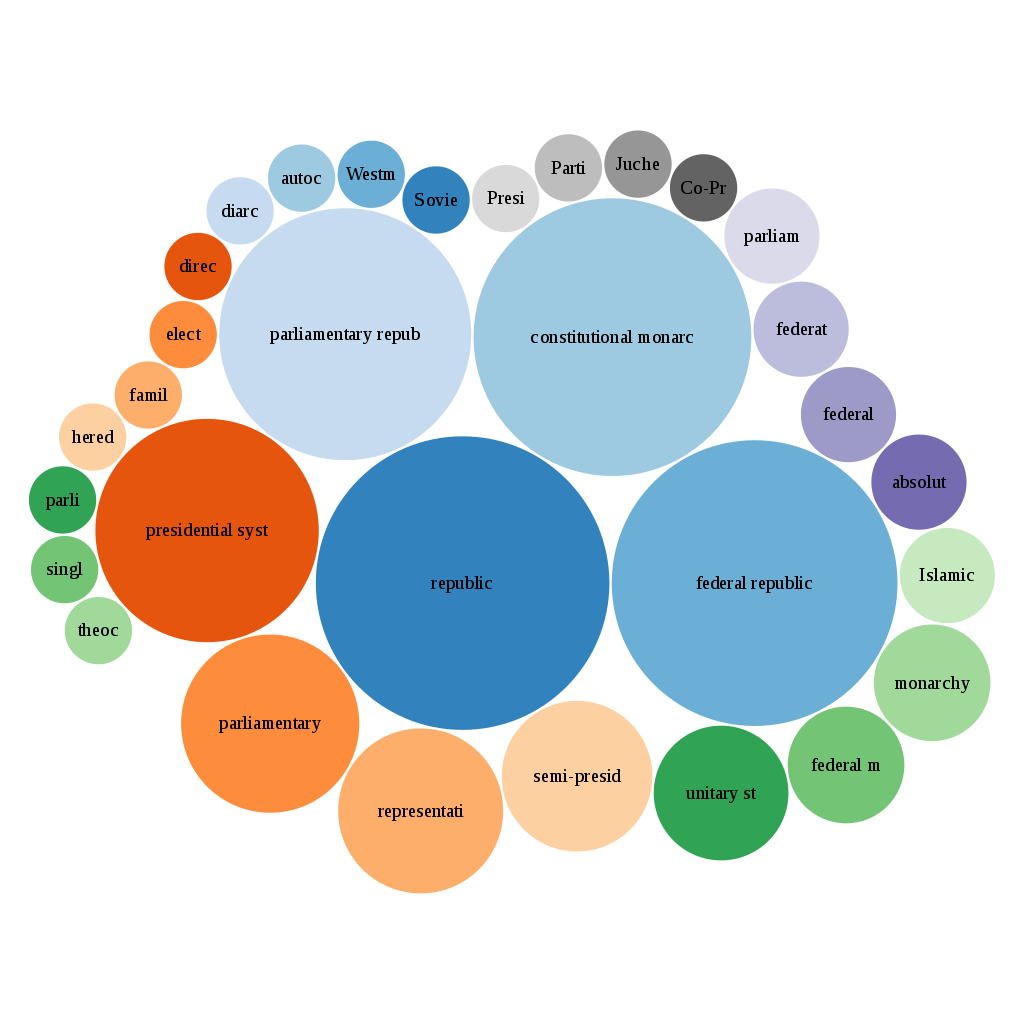
\includegraphics[width=\linewidth]{./chapter/country/Bubble_chart_forms_of_government_countries_according_to_Wikidata.png}}%
	}
	\caption{Пузырьковая диаграмма форм правления стран, 2017.
		\\			
		По данным на 2017 год основные формы правления стран: республика (в 20 странах), конституционная монархия (в 18 странах), федеративная республика (18), парламентская республика (17) и президентская республика (12).}%
	\label{fig:bubble_chart_forms_of_government_countries_2017}%
\end{figure}

\begin{figure}
	{
		\setlength{\fboxsep}{0pt}%
		\setlength{\fboxrule}{1pt}%
		\fcolorbox{gray}{gray}{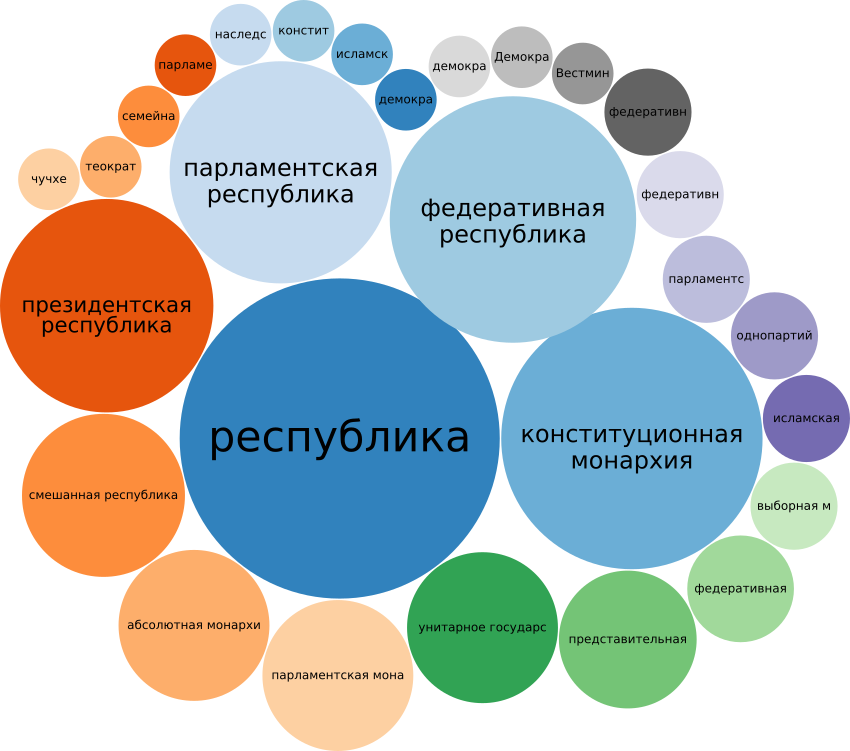
\includegraphics[width=\linewidth]{./chapter/country/Bubble_chart_forms_of_government_countries_according_to_Wikidata_2020.png}}%
	}
	\caption{Пузырьковая диаграмма форм правления стран, 2020.
	\\
	По данным на 2020 год  основные формы правления стран: республика (в 27 странах), конституционная монархия (18), федеративная республика (16), парламентская республика (13) и президентская республика (12).
}%
	\label{fig:bubble_chart_forms_of_government_countries_2020}%
\end{figure}

Таким образом, за период с 2017 по 2020 год форма правления <<республика>> стала более <<популярной>>. Значительно уменьшилось количество стран, имеющих форму  <<смешанная республика>>. Появились такие формы как демократический централизм, демократическая республика, демократия, исламское государство и парламентская демократия.

%%%%%%%%%%%%%%%%%%%%%%%%%%%%%%%%%%%%%%%%%%%%%%%%%%%%%%%
\section{Соседние страны}

Построим граф соседних стран (листинг ~\ref{lst:neighboring_countries}).
\index{График!Graph / Граф соседних стран}
\begin{lstlisting}[ language=SPARQL, 
caption={\href{https://w.wiki/k7P}{Соседние страны}\protect\footnotemark},
label=lst:neighboring_countries, 
escapebegin=ку,escapeend=ку-ку>
]
#neighboring countries graph
#defaultView:Graph
SELECT ?country ?countryLabel ?sharesBorderWith ?sharesBorderWithLabel
WHERE
{
		?country wdt:P31 wd:Q6256.	# country
		SERVICE wikibase:label { bd:serviceParam wikibase:language "ru" }
		OPTIONAL { ?country wdt:P47 ?sharesBorderWith . }
}
\end{lstlisting}

\footnotetext{Получено 787 соседств на 2017 год и 698 соседств на 2020 год. Ссылка на SPARQL-запрос: \href{https://w.wiki/k7P}{https://w.wiki/k7P}}

В результате выполнения запроса мы получаем граф с 787 ребрами на 2017 год (рис. ~\ref{fig:neighboring_countries_2017}) и 698 ребрами на 2020 год (рис. ~\ref{fig:neighboring_countries_2020}), где ребро – это соседство между двумя странами. Граф представляет из себя несколько связных компонент, так как есть островные страны, у которых нет соседей (например, Маврикий, Мальдивы, Мадагаскар).

\begin{figure}
	{
		\setlength{\fboxsep}{0pt}%
		\setlength{\fboxrule}{1pt}%
		\fcolorbox{gray}{gray}{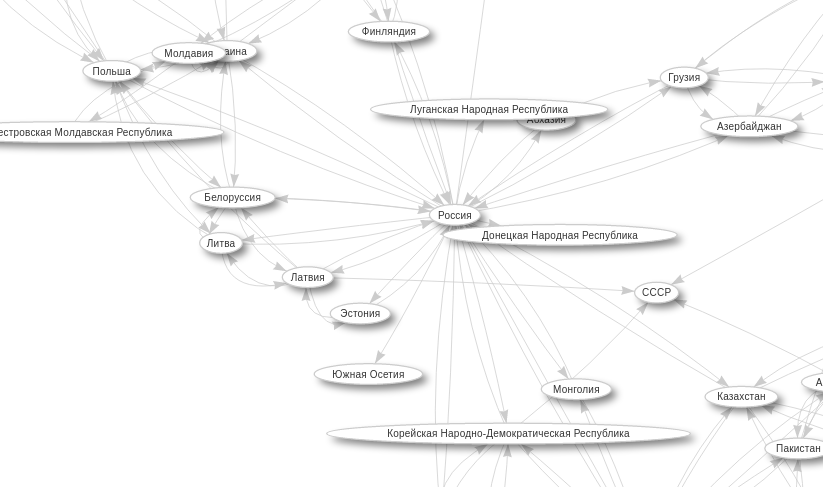
\includegraphics[width=\linewidth]{./chapter/country/Neighboring_countries_graph_in_russian_according_to_Wikidata_2017.png}}%
	}
	\caption{Фрагмент графа соседних стран, в центре Россия, 2017.
	}%
	\label{fig:neighboring_countries_2017}%
\end{figure}

\begin{figure}
	{
		\setlength{\fboxsep}{0pt}%
		\setlength{\fboxrule}{1pt}%
		\fcolorbox{gray}{gray}{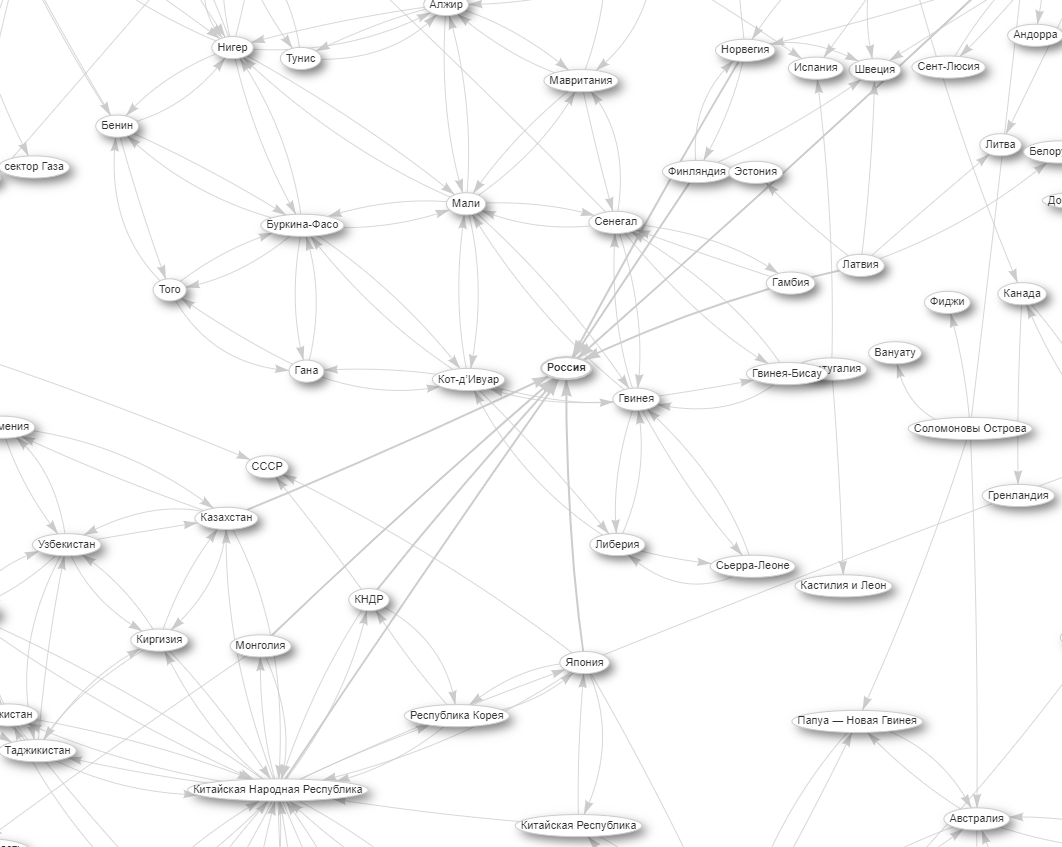
\includegraphics[width=\linewidth]{./chapter/country/Neighboring_countries_graph_in_russian_according_to_Wikidata_2020.png}}%
	}
	\caption{Фрагмент графа соседних стран, в центре Россия, 2020.
	}%
	\label{fig:neighboring_countries_2020}%
\end{figure}

\subsection{Соседние страны России}

Построим карту соседних стран России (листинг ~\ref{lst:neighboring_countries_ru}).
\index{График!Map / Карта соседних стран России}
\begin{lstlisting}[ language=SPARQL, 
caption={\href{https://w.wiki/rMP}{Соседние страны}\protect\footnotemark},
label=lst:neighboring_countries_ru, 
escapebegin=ку,escapeend=ку-ку>
]
# Map of neighboring countries of Russia
#defaultView:Map
SELECT ?border_country ?border_countryLabel ?coords ?layer
WHERE 
{
	?border_country wdt:P47 wd:Q159.  # country has border with Russia
	OPTIONAL { ?border_country wdt:P3896 ?coords. }
	BIND ( ?coords AS ?layer )
	SERVICE wikibase:label { bd:serviceParam wikibase:language "ru". }
}
\end{lstlisting}

\footnotetext{Получено 22 страны на 2020 год. Ссылка на SPARQL-запрос: \href{https://w.wiki/rMP}{https://w.wiki/rMP}}


В результате выполнения запроса мы получаем карту соседних страны России (рис. ~\ref{fig:neighboring_countries_ru_2020}), которая включает в себя следующие страны:
\begin{enumerate}
	\item \wdqName{Япония}{17}
	\item \wdqName{Норвегия}{20}
	\item \wdqName{Финляндия}{33}
	\item \wdqName{Польша}{36}
	\item \wdqName{Литва}{37}
	\item \wdqName{Китайская Народная Республика}{148}
	\item \wdqName{Белоруссия}{184}
	\item \wdqName{Эстония}{191}
	\item \wdqName{Латвия}{211}
	\item \wdqName{Украина}{212}
	\item \wdqName{Азербайджан}{227}
	\item \wdqName{Грузия}{230}
	\item \wdqName{Казахстан}{232}
	\item \wdqName{КНДР}{423}
	\item \wdqName{Европейский союз}{458}
	\item \wdqName{Монголия}{711}
	\item \wdqName{Хоккайдо}{35581}
	\item \wdqName{Рача-Лечхуми и Квемо-Сванети}{38893}
	\item \wdqName{Чеченская Республика Ичкерия}{210036}
	\item \wdqName{Донецкая Народная Республика}{16150196}
	\item \wdqName{Луганская Народная Республика}{16746854}
	\item \wdqName{Республика Абхазия}{31354462}
\end{enumerate}

\begin{figure}
	{
		\setlength{\fboxsep}{0pt}%
		\setlength{\fboxrule}{1pt}%
		\fcolorbox{gray}{gray}{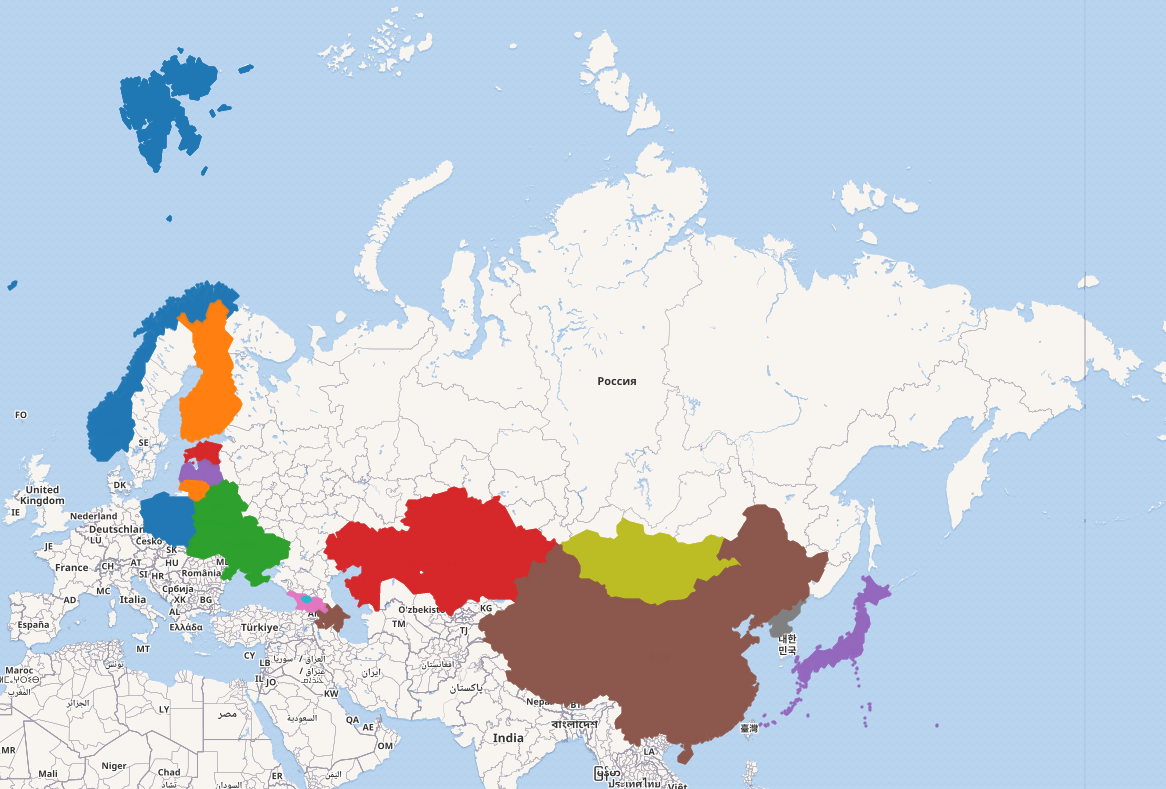
\includegraphics[width=\linewidth]{./chapter/country/Map_of_neighboring_countries_of_Russia_ru.png}}%
	}
	\caption{Карта соседних стран России, 2020.
	}%
	\label{fig:neighboring_countries_ru_2020}%
\end{figure}


%%%%%%%%%%%%%%%%%%%%%%%%%%%%%%%%%%%%%%%%%%%%%%%%%%%%%%%
\section{Упражнения}

\begin{enumerate}
	\item Постройте список флагов и девизов стран. Девизы есть не у всех стран.
	\item Отметьте на карте столицы современных стран.
	\item В каждой части света вычислите первые пять стран с наибольшей плотностью населения.
	\item Постройте столбчатую диаграмму, демонстрирующую распределение количества стран по формам правления. Оцените, является ли это распределение <<тяжелым хвостом>>.
	\item Выведите список стран упорядоченных по числу соседей. У каких стран максимальное и минимальное количество соседей, какое среднее число соседей? Есть ли корреляция между этим показателем и каким-либо другим параметром стран?
\end{enumerate}

\chapter{Населённые пункты}
\label{ch:human-settlement}

В главе исследуется объект Викиданных \wdqName{населённый пункт}{486972} и его свойства. 
В каждом из разделов представлены задачи, решённые с помощью SPARQL-запросов. 
%
%%%%%%%%%%%%%%%% Упражнение 1 %%%%%%%%%%%%%%%% 
\marginnote{Подсчитайте, сколько человек на км\textsuperscript{2} живёт в \ruwiki{4dNv}{Барабинске} 
и в~\ruwiki{4dNt}{Алейске}? В каком из этих \emph{населённых пунктов} плотность населения выше?

См. ответ~\ref{answer:human_settlements_density} на с.~\pageref{answer:human_settlements_density}.%
}

Был получен список населённых пунктов, 
построены пузырьковые диаграммы с количеством населения в <<населённых пунктах>> по странам. 
Построена диаграмма, показывающая долю населения, 
проживающего в населённых пунктах относительно всего населения страны. 
Диаграмма показала, что высокий процент населения, проживающего в населённых пунктах, 
приходится на сельскохозяйственные страны, в то время как в более индустриальных странах 
меньшая доля населения проживает в населённых пунктах. 

%%%%%%%%%%%%%%%% Упражнение 2 %%%%%%%%%%%%%%%%
\marginnote{Выберите, представленный герб относится к населённым пунктам Российской Федерации или нет, изображенный на рис. \ref{fig:flag_question_human_settlements1}? }
\begin{marginfigure}[0.0cm] {
\setlength{\fboxsep}{0pt}%
\setlength{\fboxrule}{1pt}%
\fcolorbox{gray}{gray}{
\includegraphics[width=0.5\linewidth]{./chapter/human_settlement/Aznakeevskii_rayon_gerb.png}}%
}
  \caption{Герб населённого пункта.}%
  \label{fig:flag_question_human_settlements1}%
\end{marginfigure}

\marginnote{
См. ответ~\ref{answer:flag_human_settlements} на с.~\pageref{answer:flag_human_settlements}.
}
На 2017 год Википедия описывала примерно половину населённых пунктов (75 тыс.), 
Викиданные содержали менее 3\% таких поселений (4 тыс.) относительно данных переписи за 2010 год (155,5 тыс.). 
На 2021 год Викиданные содержат менее 12\% таких поселений (17 тыс.) 
относительно данных той же переписи за 2010 год. 

Для сравнения сельских и городских поселений 
построены диаграммы количества учёных, сгруппированных по родам деятельности, 
и разбитых по месту рождения: сельское или городское.

Для поиска более полных ответов на поставленные выше задачи  
были найдены более общие классы для объекта \wdqName{населённый пункт}{486972} 
с помощью свойства \wdProperty{31}{частный случай понятия}. 
Трудность исследования вызвана отсутствием чёткой типологии населённых пунктов 
(например, от численности населения) в законодательстве России и в Викиданных.

%%%%%%%
\section{Список <<Населённых пунктов>>}

Для построения списка всех населённых пунктов нам потребуются объект \wdqName{населённый пункт}{486972} и свойство \wdProperty{31}{экземпляр} (листинг ~\protect\ref{lst:human-settlement1}).

\begin{lstlisting}[ language=SPARQL, 
                    caption={\href{https://w.wiki/4d7x}{Список всех населённых пунктов}\protect\footnotemark},
                    label=lst:human-settlement1,
                    texcl 
                    ]
# List of all human settlements
SELECT ?hum ?humLabel WHERE{
  ?hum wdt:P31 wd:Q486972. # instance of human settlement
  SERVICE wikibase:label{bd:serviceParam wikibase:language "ru,en"}
}
\end{lstlisting}%
\footnotetext{Получен \num{411393} записи в 2017 году.  Ссылка на SPARQL-запрос: \href{https://w.wiki/4d7x}{https://w.wiki/4d7x}}

В 2021 году оказалось не возможно получить список населённых пунктов из-за большого числа объектов и поэтому слишком долгой работы (листинг ~\protect\ref{lst:human-settlement1}). Для получения результата произведём подсчёт всех населённых пунктов с помощью функции \textit{COUNT()} (листинг ~\protect\ref{lst:human-settlement2}).

\index{SPARQL!COUNT!Количество всех населённых пунктов}
\begin{lstlisting}[ language=SPARQL, 
                    caption={\href{https://w.wiki/4d7s}{Количество всех населённых пунктов}\protect\footnotemark},
                    label=lst:human-settlement2,
                    texcl 
                    ]
# Number of human settlements
SELECT (COUNT(?hum) AS ?count) WHERE {
  ?hum wdt:P31 wd:Q486972. # instance of human settlement  
}
\end{lstlisting}%
\footnotetext{Получили \num{563126} населённых пунктов в 2021 году. Ссылка на SPARQL-запрос: \href{https://w.wiki/4d7s}{https://w.wiki/4d7s}}

Почти пустыми и малоинформативными оказались такие населёнными пункты: \wdqName{Zangabad}{146827} (2 свойства) и \wdqName{Zapallar}{147201} (2 свойства). Среди отечественных населённых пунктов: \wdqName{Borisovo}{4093951} (3 свойства) и \wdqName{Zakhod}{18777794} (3 свойства).

Среди населённых пунктов принадлежащих России в Викиданных больше всего свойств по данным ProWD у \href{http://www.wikidata.org/entity/Q128499}{Ялты} (36 свойств). Лидером по всему миру является \href{http://www.wikidata.org/entity/Q1490}{Токио} (73 свойства)\autocite{humansettlements_ProWD}.

%%%%%%%
\section{Список стран по суммарному количеству населения}

Построим упорядоченный список стран по суммарному количеству населения, проживающего в <<населённых пунктах>> (листинг ~\protect\ref{lst:human-settlement3}).

%%%%%%%%%%%%%%%% Упражнение 2 %%%%%%%%%%%%%%%%
\marginnote{
Выберите, представленный герб относится к населённым пунктам Российской Федерации или нет, изображенный на рис. \ref{fig:flag_question_human_settlements2}?
}
\begin{marginfigure}[0.0cm]
{
\setlength{\fboxsep}{0pt}%
\setlength{\fboxrule}{1pt}%
\fcolorbox{gray}{gray}{
\includegraphics[width=0.5\linewidth]{./chapter/human_settlement/Coat_of_Arms_of_Asbest_(Sverdlovsk_oblast).png}}%
}
  \caption{Герб населённого пункта.}%
  \label{fig:flag_question_human_settlements2}%
\end{marginfigure}

\marginnote{
См. ответ~\ref{answer:flag_human_settlements} на с.~\pageref{answer:flag_human_settlements}.
}

\index{SPARQL!SUM!Список стран по суммарному количеству населения, проживающего в <<населённых пунктах>>}
\index{SPARQL!GROUP BY!Список стран по суммарному количеству населения, проживающего в <<населённых пунктах>>}
\lstset{numbers=left, firstnumber=1, frame=single}
\begin{lstlisting}[ language=SPARQL, 
                    caption={\href{https://w.wiki/4d9M}{Список стран по суммарному количеству населения, проживающего в <<населённых пунктах>>}\protect\footnotemark},
                    label=lst:human-settlement3,
                    texcl 
                    ]
# List of countries by population in settlements
SELECT ?country ?countryLabel (SUM(?population) as ?sumPopulation)
WHERE {
  ?hum wdt:P31 wd:Q486972;  	# instance of human settlement
       wdt:P17 ?country;    	# in the ?country
       wdt:P1082 ?population. # has ?population
  SERVICE wikibase:label{bd:serviceParam wikibase:language "ru,en"}
}
GROUP BY ?country ?countryLabel 
ORDER BY DESC (?sumPopulation)
\end{lstlisting}%
\footnotetext{Получена \num{161} страна в 2017 году и \num{213} стран в 2021 году. Ссылка на SPARQL-запрос: \href{https://w.wiki/4d9M}{https://w.wiki/4d9M}}

Для подсчета насления по странам, используем команду \textit{SUM()} на второй строке скрипта (листинг ~\protect\ref{lst:human-settlement3}). Для группировки населённых пунктов по странам, используем команду \textit{GROUP BY} на девятой строке скрипта (листинг ~\protect\ref{lst:human-settlement3}).

Пузырьковая диаграмма на рис. ~\ref{fig:human-settlement-1} показывает соотношение стран по количеству населения в <<населённых пунктах>> в 2017 году.

\begin{figure}
\centering
	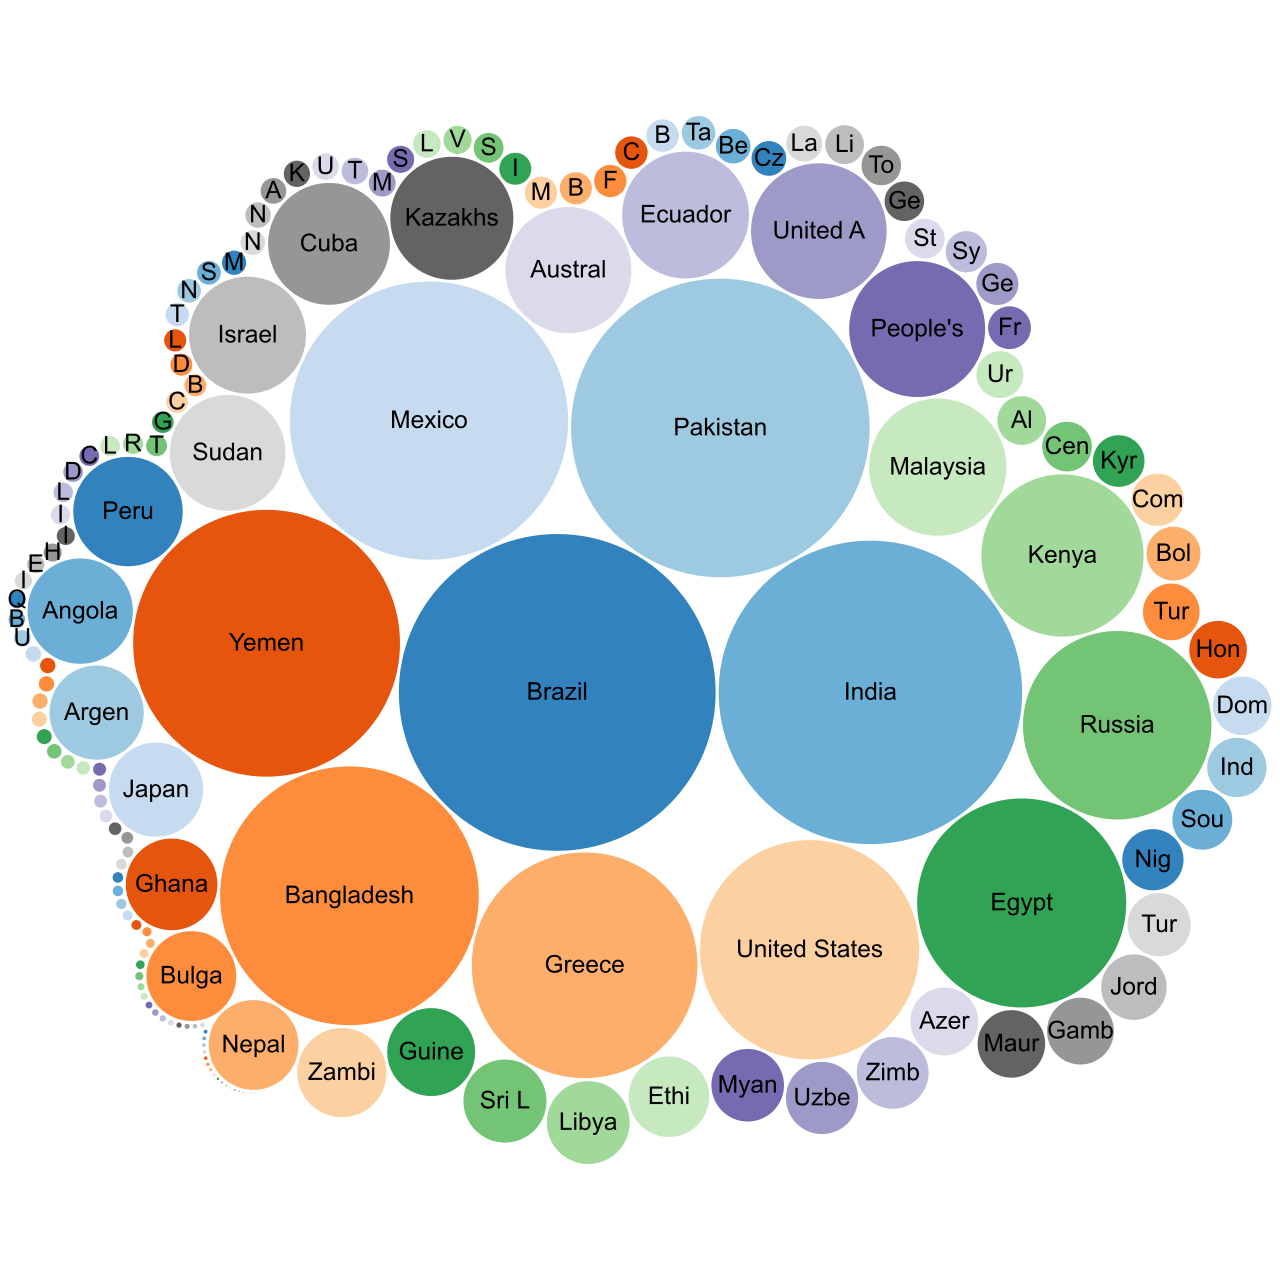
\includegraphics[width=0.9\linewidth]{./chapter/human_settlement/AnnaBubbleHumanSettlement.jpg}
	\label{fig:human-settlement-1}
    \caption[Пузырьковая диаграмма  по суммарному количеству населения в населённых пунктах, 2017.]{Пузырьковая диаграмма  по суммарному количеству населения, проживающего в <<населённых пунктах>> на 2017 год. Размер пузырька соответствует количеству населения, проживающего в <<населённых пунктах>> одной страны. Ссылка на SPARQL-запрос: \href{https://w.wiki/4dAv}{https://w.wiki/4dAv}}
\end{figure}

\begin{figure}
\centering
	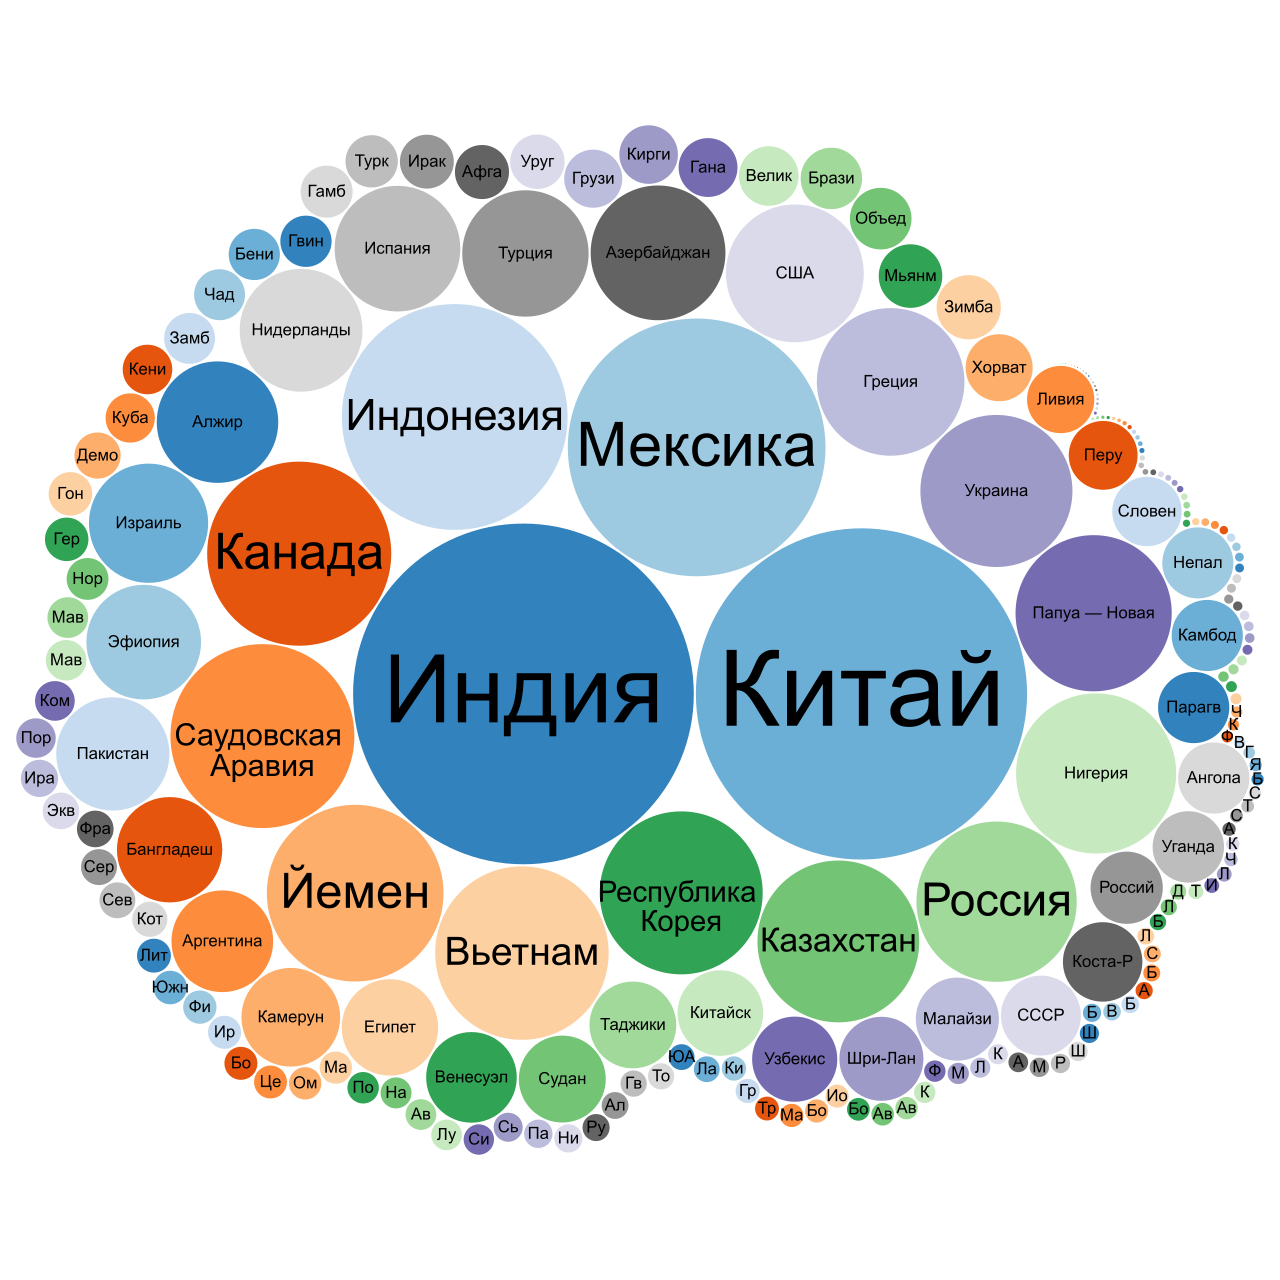
\includegraphics[width=0.9\linewidth]{./chapter/human_settlement/LeonidBubbleHumanSettlement.jpg}
	\label{fig:human-settlement-2}
	\caption[Пузырьковая диаграмма  по суммарному количеству населения в населённых пунктах, 2021.]{Пузырьковая диаграмма  по суммарному количеству населения, проживающего в <<населённых пунктах>> на 2021 год. Размер пузырька соответствует количеству населения, проживающего в <<населённых пунктах>> одной страны. Ссылка на SPARQL-запрос: \href{https://w.wiki/4dAv}{https://w.wiki/4dAv}}
\end{figure}

В 2017 году больше всего количество населения проживало в объектах <<населённый пункт>> в таких странах, как: \href{http://www.wikidata.org/entity/Q155}{Бразилия} (\num{12} млн), \href{http://www.wikidata.org/entity/Q843}{Пакистан} (\num{10} млн), \href{http://www.wikidata.org/entity/Q96}{Мексика} (\num{8} млн), \href{http://www.wikidata.org/entity/Q805}{Йемен} (\num{8} млн), \href{http://www.wikidata.org/entity/Q668}{Индия} (\num{7} млн), \href{http://www.wikidata.org/entity/Q902}{Бангладеш} (\num{7} млн). 

На рис. ~\ref{fig:human-settlement-2} можно увидеть список стран на 2021 год: \href{http://www.wikidata.org/entity/Q668}{Индия} (\num{30} млн), \href{http://www.wikidata.org/entity/Q148}{Китай} (\num{28} млн), \href{http://www.wikidata.org/entity/Q96}{Мексика} (\num{17} млн), \href{http://www.wikidata.org/entity/Q252}{Индонезия} (\num{13} млн), \href{http://www.wikidata.org/entity/Q16}{Канада} (\num{9} млн), \href{http://www.wikidata.org/entity/Q851}{Саудовская Аравия} (\num{9} млн). 

Итоги запросов в 2017 и 2021 имеют сильно разные результаты. За четыре года в Индии прибавилось 23 млн человек, из этого можно сделать вывод, что за четыре года информация в Викиданных стала более полной по населённым пунктам.

%%%%%
\subsection{Полнота Викиданных}

Населённый пункт — это общее название мест с постоянными жителями\autocite{Humansettlements_Dictionary}. По версии редакторов Викиданных в понятие насёленный пункт входят города, сёла, деревни и другие\footnote{Полный список можно увидеть в разделе <<Cписок классов, сопутствующих <<населённому пункту>> в свойстве <<экземпляр>>>> на с.~\pageref{human-settlement:tag1}.}.
Точной информации о количестве населённых пунктов в мире не было найдено. Поэтому проверим полноту населённых пунктов, которые есть в Викиданных и которые использовались для решения задачи. В задачах выше мы использовали свойста \wdProperty{1082}{численность населения} и \wdProperty{17}{государство} (привязанность к стране). Исходя из этого проверку полноты разделим на подзадачи: 
\begin{enumerate} 
  \item Проверка заполнености свойства <<численность населения>>.
  \item Проверка принадлежности к <<государству>>.
\end{enumerate}

%%%%%
\subsection{Проверка заполнености свойства <<численность населения>> }

Для этого напишем \href{https://w.wiki/4FUz}{SPARQL-запрос}\footnotemark, который выведет населённые пункты с незаполненным свойством \href{http://www.wikidata.org/entity/P1082}{численность населения}. 
\footnotetext{ В 2017 году запрос выдал \num{372997} населённых пунктов с незаполненным свойством <<численность населения>>. Проводя ту же проверку в 2021 году, запрос выдал \num{507078} таких населённых пунктов. Ссылка на SPARQL-запрос: \href{https://w.wiki/4FUz}{https://w.wiki/4FUz}} 
Произведя расчеты получаем, что только у 9,3\% населенных пунктов мира указано свойство <<численность населения>> на 2017 год. В 2021 получаем 11,2\% населенных пунктов мира с заполненным свойство <<численность населения>>.

%%%%%
\subsection{Проверка принадлежности к <<государству>>}

А теперь посмотрим населённые пункты, у которых не указана принадлежность к какой-либо стране~--- \href{https://w.wiki/4FV8}{SPARQL-запрос}\footnotemark.

\footnotetext{В 2017 году нашлось \num{8427} объектов, у которых не указана принадлежность к какой-либо стране. В 2021 году таких объектов уже больше~--- \num{27824}. Ссылка на SPARQL-запрос: \href{https://w.wiki/4FV8}{https://w.wiki/4FV8}}
Получалется неполная картина при получении результата решения данной задачи о суммарном количестве населения в населённых пунктах по странам из-за того, что такие объекты существуют.

%%%%%
\section{Доля населения страны, проживающего в <<населённых пунктах>>}

Построим упорядоченный список стран доли населения (в процентах), проживающего в \href{http://www.wikidata.org/entity/Q486972}{населённых пунктах}, относительно числа всех жителей страны (листинг ~\protect\ref{lst:human-settlement6}).

%%%%%%%%%%%%%%%% Упражнение 2 %%%%%%%%%%%%%%%%
\marginnote{
Выберите, представленный герб относится к населённым пунктам Российской Федерации или нет, изображенный на рис. \ref{fig:flag_question_human_settlements3}?
}
\begin{marginfigure}[0.0cm]
{
\setlength{\fboxsep}{0pt}%
\setlength{\fboxrule}{1pt}%
\fcolorbox{gray}{gray}{
\includegraphics[width=0.5\linewidth]{./chapter/human_settlement/Loučovice_CoA.jpg}}%
}
  \caption{Герб населённого пункта.}%
  \label{fig:flag_question_human_settlements3}%
\end{marginfigure}

\marginnote{
См. ответ~\ref{answer:flag_human_settlements} на с.~\pageref{answer:flag_human_settlements}.
}

\index{SPARQL!SUM!Соотношение количества людей, проживающих в населённых пунктах, к количеству всех людей в стране}
\begin{lstlisting}[ language=SPARQL, 
                    caption={\href{https://w.wiki/4dE3}{Соотношение количества людей, проживающих в населённых пунктах, к количеству всех людей в стране}\protect\footnotemark},
                    label=lst:human-settlement6,
                    texcl 
                    ]
# An ordered list of the ratio of the number of people living in 
# "human\_settlement" to the number of inhabitants in the country.
SELECT ?country ?countryLabel ?proportionPopulation WHERE {
 SELECT ?country ?countryLabel (SUM(?population / ?pop) 
        as ?proportionPopulation) WHERE {
  ?hum wdt:P31 wd:Q486972;    # instances of human settlement  
       wdt:P17 ?country;         # has ?country 
       wdt:P1082 ?population.    # has ?population
  ?country wdt:P1082 ?pop.    # population in the country
  SERVICE wikibase:label{bd:serviceParam wikibase:language "ru,en"}
 }
 GROUP BY ?country ?countryLabel
}
ORDER BY ?proportionPopulation
\end{lstlisting}%
\footnotetext{Получено \num{158} результатов в 2017 году и \num{206} результатов в 2021 году. Ссылка на SPARQL-запрос: \href{https://w.wiki/4dE3}{https://w.wiki/4dE3}}

Столбчатая диаграмма на рис. ~\ref{fig:human-settlement-3} позволяет увидеть для каждой отдельной страны отношение количества людей, проживающих в \href{http://www.wikidata.org/entity/Q486972}{населённых пунктах}, к числу жителей в стране на 2017 год.

\begin{figure*}
    \setlength{\fboxsep}{0pt}%
    \setlength{\fboxrule}{1pt}%
    \fcolorbox{gray}{gray}{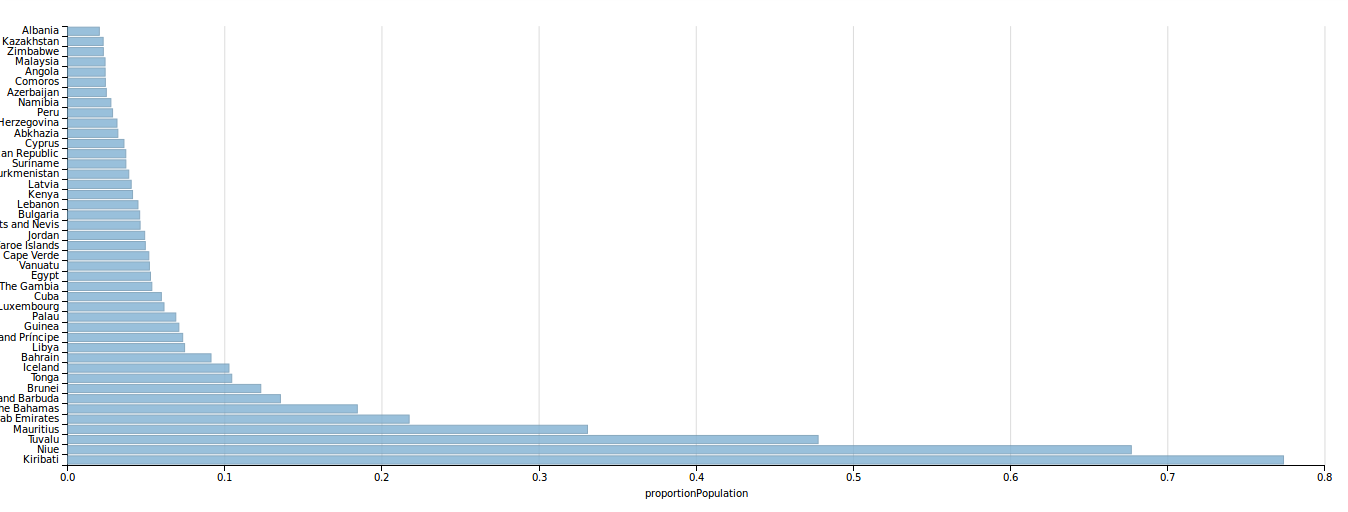
\includegraphics[width=1\linewidth]{./chapter/human_settlement/AnnaShareHumanSettlement.png}}
	\label{fig:human-settlement-3}
	\caption[Диаграмма доли населения страны, 2017.]{Диаграмма доли населения страны, проживающего в <<населённых пунктах>> на 2017 год. Ссылка на SPARQL-запрос: \href{https://w.wiki/4dE3}{https://w.wiki/4dE3}}%
\end{figure*} 

\begin{figure*}
    \setlength{\fboxsep}{0pt}%
    \setlength{\fboxrule}{1pt}%
    \fcolorbox{gray}{gray}{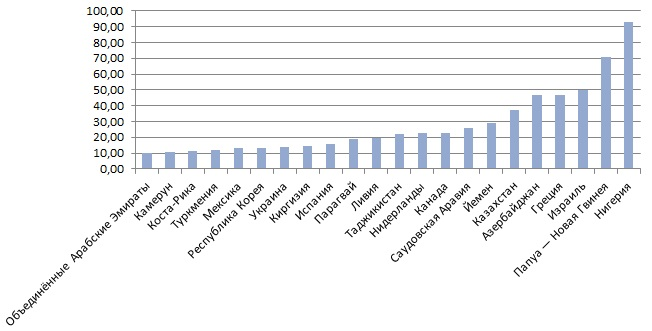
\includegraphics[width=1\linewidth]{./chapter/human_settlement/LeonidShareHumanSettlement.jpg}}
	\label{fig:human-settlement-4}
	\caption[Диаграмма доли населения страны, 2021.]{Диаграмма доли населения страны, проживающего в <<населённых пунктах>> на 2021 год. В 2021 на диаграмму попали только страны с населением более 5 млн человек. Ссылка на SPARQL-запрос: \href{https://w.wiki/4dDx}{https://w.wiki/4dDx}}%
\end{figure*} 

На рис. ~\ref{fig:human-settlement-3} из графика видно, что наиболее высокий процент в 2017 году приходился на следующие страны: Кирибати (78\%), Ниуэ (70\%), Греция (53\%), Тувалу (48\%), Коморы (43\%), Маврикий (42\%). В 2021 году появились изменения : Нигерия (93\%), Папуа — Новая Гвинея (71\%), Израиль (50\%), Греция (47\%), Азербайджан (47\%), Казахстан (37\%). Интересно заметить, что в основном это маленькие островные государства. Вероятно, большая часть жителей этих стран сконцентрирована в населённых пунктах.

На 2017 год рассматривая отдельно страны большой восьмёрки, доля жителей в \href{http://www.wikidata.org/entity/Q486972}{населённых пунктах} составила: \href{http://www.wikidata.org/entity/Q159}{Россия} (\num{2.98}\%), \href{http://www.wikidata.org/entity/Q30}{США} (\num{1.76}\%), \href{http://www.wikidata.org/entity/Q17}{Япония} (\num{0.80}\%), \href{http://www.wikidata.org/entity/Q16}{Канада} (\num{0.26}\%), \href{http://www.wikidata.org/entity/Q142}{Франция} (\num{0.20}\%), \href{http://www.wikidata.org/entity/Q183}{Германия} (\num{0.24}\%), \href{http://www.wikidata.org/entity/Q145}{Великобритания} (\num{0.18}\%), \href{http://www.wikidata.org/entity/Q38}{Италия} (\num{0.07}\%). В 2021 году значения доли населения снизились: \href{http://www.wikidata.org/entity/Q159}{Россия} (0.045\%), \href{http://www.wikidata.org/entity/Q30}{США} (\num{0.014}\%), \href{http://www.wikidata.org/entity/Q17}{Япония} (\num{0.008}\%), \href{http://www.wikidata.org/entity/Q16}{Канада} (\num{0.23}\%), \href{http://www.wikidata.org/entity/Q142}{Франция} (\num{0.005}\%), \href{http://www.wikidata.org/entity/Q183}{Германия} (\num{0.005}\%), \href{http://www.wikidata.org/entity/Q145}{Великобритания} (\num{0.014}\%), \href{http://www.wikidata.org/entity/Q38}{Италия} (\num{0.0005}\%). Отметим, что это страны промышленно развитые.

%%%%%%%%%%%%%%%% Упражнение 2 %%%%%%%%%%%%%%%%
\marginnote{
Выберите, представленный герб относится к населённым пунктам Российской Федерации или нет, изображенный на рис. \ref{fig:flag_question_human_settlements4}?
}
\begin{marginfigure}[0.0cm]
{
\setlength{\fboxsep}{0pt}%
\setlength{\fboxrule}{1pt}%
\fcolorbox{gray}{gray}{
\includegraphics[width=0.5\linewidth]{./chapter/human_settlement/POL_Otynia_COA.png}}%
}
  \caption{Герб населённого пункта.}%
  \label{fig:flag_question_human_settlements4}%
\end{marginfigure}

\marginnote{
См. ответ~\ref{answer:flag_human_settlements} на с.~\pageref{answer:flag_human_settlements}.
}

Построенная диаграмма подтверждает следующую гипотезу: высокий процент населения страны, проживающего в \wdqName{населённых пунктах}{486972}, указывает на более аграрную страну. Исходя из представленных выше диаграмм видно, что наиболее высокий процент населения страны, проживающего в населённых пунктах, приходится на островные, южные, жаркие страны, в которых, по-видимому, менее развита промышленность (маленькая территория, небольшое количество населения, удалённость от материков). А индустриальные страны (большой восьмёрки) имеют очень низкий процент населения страны, проживающего в населённых пунктах.

%%%%%
\section{Cписок классов, сопутствующих <<населённому пункту>> в свойстве <<экземпляр>>}
\label{human-settlement:tag1}

Далее классом будем называть каждый элемент в исследуемом объекте на Викиданных, связанный через свойство \wdProperty{31}{экземпляра}. Главная цель этого раздела, получить классы в свойстве <<экземпляр>>, используемые совместно с классом \wdqName{населённый пункт}{486972}. Такие классы будем считать сопутсвующими. Для этого попробуем получить список объектов, имеющих свойство <<населённый пункт>> (листинг ~\protect\ref{lst:human-settlement7}).

Далее классом будем называть каждый элемент в исследуемом объекте на Викиданных, связанный через свойство \wdProperty{31}{экземпляра}

%%%%%%%%%%%%%%%% Упражнение 2 %%%%%%%%%%%%%%%%
\marginnote{
Выберите, представленный герб относится к населённым пунктам Российской Федерации или нет, изображенный на рис. \ref{fig:flag_question_human_settlements5}?
}
\begin{marginfigure}[0.0cm]
{
\setlength{\fboxsep}{0pt}%
\setlength{\fboxrule}{1pt}%
\fcolorbox{gray}{gray}{
\includegraphics[width=0.5\linewidth]{./chapter/human_settlement/Coat_of_Arms_of_Azov.png}}%
}
  \caption{Герб населённого пункта.}%
  \label{fig:flag_question_human_settlements5}%
\end{marginfigure}

\marginnote{
См. ответ~\ref{answer:flag_human_settlements} на с.~\pageref{answer:flag_human_settlements}.
}

\begin{lstlisting}[ language=SPARQL, 
                    caption={\href{https://w.wiki/4dEW}{Cписок классов, сопутствующих <<населённому пункту>> в свойстве <<экземпляр>>}\protect\footnotemark},
                    label=lst:human-settlement7,
                    texcl 
                    ]
# List of classes accompanying the human\_settlement in the
# property 'instance of'
SELECT ?inst (COUNT(?hum) as ?sumHum) 
WHERE{          
  ?hum wdt:P31 wd:Q486972; # instance of human settlement
       wdt:P31 ?inst.      # other objects in instance
  SERVICE wikibase:label{bd:serviceParam wikibase:language "ru,en"}
}  
GROUP BY ?inst
\end{lstlisting}%
\footnotetext{Получено 610 результатов в 2017 году и \num{1245} результатов в 2021 году. Ссылка на SPARQL-запрос: \href{https://w.wiki/4dEW}{https://w.wiki/4dEW}}

Для ускорения выполнения (листинг ~\protect\ref{lst:human-settlement7}) выполним следующие два шага.
 
Во-первых, выключим из рассмотрения такие поселения, которые имеют в списке экземпляров только <<населённый пункт>>. Результат не ухудшится, так как в него не будут включёны экземпляры только класса <<населённый пункт>>. С этой целью внесём в наш скрипт строку \num{9} и получим фильтр для отбора нужных поселений.

Во-вторых, в строке \num{8} уберем такие объекты переменной \emph{?inst}, которые имеют свойство \wdqName{государство}{17}. Это позволит отсечь сотни типов населённых пунктов специфичных для отдельных стран, например, административно-территориальная единица России.

Эти перобразования позволили выполнить запрос по всем странам мира за приемлемое время (13 мс) (листинг ~\protect\ref{lst:human-settlement8}).

\lstset{numbers=left, firstnumber=1, frame=single}
\begin{lstlisting}[ language=SPARQL, 
                    caption={\href{https://w.wiki/4dTx}{Cписок классов, сопутствующих <<населённому пункту>> в свойстве <<экземпляр>>, без специфичных для отдельных стран}\protect\footnotemark},
                    label=lst:human-settlement8,
                    texcl 
                    ]
# List of objects with the class of human settlement, without 
# country and single human settlement
SELECT ?inst (COUNT(?hum) as ?sumHum) 
WHERE{ 
  ?hum wdt:P31 wd:Q486972;  # instance of human settlement
       wdt:P31 ?inst.       # other objects in instance
  
  MINUS {?inst wdt:P17 []}. # without country
  FILTER(?inst != wd:Q486972 ). # without human settlement
  SERVICE wikibase:label{bd:serviceParam wikibase:language "ru,en"}
}  
GROUP BY ?inst 
ORDER BY DESC (?sumHum)
\end{lstlisting}%
\footnotetext{Получено 355 записей в 2017 году и 707 записей в 2021 году. Ссылка на SPARQL-запрос: \href{https://w.wiki/4dTx}{https://w.wiki/4dTx}}

В таблице~\ref{tab:human-settlement2} представлены сравнительные результаты между 2017  и 2021 годами, количества классов, сопутствующих <<населённому пункту>> в свойстве <<экземпляр>>.

\begin{table}[h]
\centering
\begin{tabular}{|l|l|l|l|l|}
\hline
номер & название класса                       				& количество на 2017	& количество на 2021 	& разница		\\ \hline
1         & \wdqName{Cёло}{532}     					& \num{2844}                	& \num{4853}		& +\num{2009}	\\
2         & \wdqName{Муниципалитеты}{15284}              		& \num{1181}                	& \num{3376}		& +\num{2195}	\\
3         & \wdqName{Деревни}{5084}					& \num{662}               	& \num{1761}		& +\num{1099}	\\ 
4         & \wdqName{Археологические памятники}{839954}	& \num{425}               	& \num{887}			& +\num{462}	\\ 
5         & \wdqName{Местные поселения}{3257686}		& \num{425}               	& \num{158}			& -\num{257}	\\ 
6         & \wdqName{Разрушенные города}{14616455}     		& \num{423}                	& \num{388}			& -\num{40}	\\
7         & \wdqName{Города}{515}              				& \num{322}                	& \num{545}			& +\num{223}	\\
8         & \wdqName{Малые города}{3957}				& \num{277}               	& \num{446}			& +\num{169}	\\ 
9         & \wdqName{Заброшенные деревни}{350895}		& \num{254}               	& \num{474}			& +\num{220}	\\ 
10       & \wdqName{Внутренние районы}{2983893}		& \num{207}               	& \num{503}			& +\num{296}	\\ \hline
\end{tabular}
\caption{Сравнительные результаты между 2017  и 2021 годами, количества классов, сопутствующих <<населённому пункту>> в свойстве <<экземпляр>>}
\label{tab:human-settlement2}
\end{table}

В 2021 году была преложена ещё одна модернизация (листинг ~\protect\ref{lst:human-settlement7}). А именно: отсечь доисторические поселения таких типов, как поселения \wdqName{латенского периода}{106505016}, \wdqName{бронзового века}{106491277} и \wdqName{доисторического времени, где есть письменность}{106505070}, без явного указания этих трёх объектов. 

Что есть общего у этих трех объектов на Викиданных? Они являются подклассами объектов, которые, в свою очередь, являются экземпляром объектов \wdqName{археологической культуры}{465299}, \wdqName{исторического периода}{11514315}, \wdqName{археологического века}{15401699}, \wdqName{всемирной истории}{200325} и \wdqName{геологического периода}{392928}. Применяя фильтр с описаным выше подклассам получаем такой результат (листинг ~\protect\ref{lst:human-settlement9}).

\index{SPARQL!COUNT!Cписок классов, сопутствующих <<населённому пункту>> в свойстве <<экземпляр>>, без исторических объектов}
\index{SPARQL!FILTER!Cписок классов, сопутствующих <<населённому пункту>> в свойстве <<экземпляр>>, без исторических объектов}
\index{SPARQL!MINUS!Cписок классов, сопутствующих <<населённому пункту>> в свойстве <<экземпляр>>, без исторических объектов}
\lstset{numbers=left, firstnumber=1, frame=single}
\begin{lstlisting}[ language=SPARQL, 
                    caption={\href{https://w.wiki/4dTq}{Cписок классов, сопутствующих <<населённому пункту>> в свойстве <<экземпляр>>, без исторических объектов}\protect\footnotemark},
                    label=lst:human-settlement9,
                    texcl 
                    ]
# List of classes accompanying the human\_settlement in the property
# 'instance of' without historical objects 
SELECT ?inst ?instLabel (COUNT(?hum) as ?sumHum) WHERE{
  ?hum wdt:P31 wd:Q486972;    # instance of human settlement
       wdt:P31 ?inst. # other objects in instance of human settlement
  ?inst wdt:P31 ?test. # instance of ?inst
  ?test wdt:P31 ?typ. # instance of ?test
  MINUS {?inst wdt:P17 []}.   # without country
  # without human settlement and prehistoric settlements
  FILTER(?inst != wd:Q486972 && ?typ != wd:Q465299 
         && ?typ != wd:Q11514315 && ?typ != wd:Q15401699 
         && ?typ != wd:Q200325 && ?typ != wd:Q392928 ). 
  SERVICE wikibase:label{bd:serviceParam wikibase:language "ru,en"}
}
GROUP BY ?inst ?instLabel
ORDER BY DESC (?sumHum)
\end{lstlisting}%
\footnotetext{Получено 89 результатов. Ссылка на SPARQL-запрос: \href{https://w.wiki/4dTq}{https://w.wiki/4dTq}}

В итоге, вместо 707 классов из (листинг ~\protect\ref{lst:human-settlement8}), мы получили 89 различных классов, сопутствующих <<населённому пункту>> в свойстве <<экземпляр>> . 

%%%%%
\section{Отечественные учёные на селе и в городе}

Попробуем подсчитать число отечественных учёных, родившихся в сельских и городских типах населённых пунктов. И сравнить эти числа.
Решим эту задачу за пять шагов:
\begin{enumerate}
  \item Выявим список сельских и список городских типов поселений именно в России.
  \item Определим основные научные направления, представленные в Викиданных.
  \item Выявим способ определения отечественных ученых.
  \item Сделаем такую диаграмму, на которой разным цветом будут указаны разные научные направления (математики, физики, химики и так далее) для учёных родившихся в сельских поселениях.
  \item Сделаем вторую диаграмму — по городским поселениям и сравнить результаты.
\end{enumerate}

%%%%%
\subsection{Список сельских и список городских типов поселений именно в России}

Выведем список классов поселений и их количество для объектов имеющих свойство \wdProperty{1082}{численность населения} и принадлежащие государству \wdqName{России}{159} (листинг ~\protect\ref{lst:human-settlement4}). 

\index{SPARQL!COUNT!Список классов поселений и их количество для объектов имеющих свойство <<численность населения>> в России}
\begin{lstlisting}[ language=SPARQL, 
                    caption={\href{https://w.wiki/4dBU}{Список классов поселений и их количество для объектов имеющих свойство <<численность населения>> в России}\protect\footnotemark},
                    label=lst:human-settlement4,
                    texcl 
                    ]
# List of settlement classes and their number for objects with 
# the property "population" in Russia
SELECT ?class ?classLabel (COUNT(?class) AS ?count) WHERE {
  {
  SELECT ?class ?classLabel ?humLabel WHERE {
   ?hum wdt:P17 wd:Q159;  # settlement in the Russia
        wdt:P1082 ?population; # has ?population
        wdt:P31 ?class. # has ?class
    SERVICE wikibase:label{bd:serviceParam wikibase:language "ru,en"}
   }
  }
}
GROUP BY ?class ?classLabel
ORDER BY DESC (?count)
\end{lstlisting}%
\footnotetext{Получили 216 разных классов поселений. Ссылка на SPARQL-запрос: \href{https://w.wiki/4dBU}{https://w.wiki/4dBU}}

Основные классы (листинг ~\protect\ref{lst:human-settlement4}) представлены в таблице ~\ref{tab:human-settlement1}.

\begin{table}[h]
\centering
\begin{tabular}{|l|l|l|l|}
\hline
номер & название класса                       						& количество упоминаний	& Население		\\ \hline
1         & \wdqName{сельское поселение в России}{634099}     			& \num{18104}                		& \num{34043885} 		\\
2         & \wdqName{деревня}{5084}              						& \num{14795}                		& \num{1727221}       	\\
3         & \wdqName{село}{532}								& \num{9875}               		& \num{10584016} 		\\ 
4         & \wdqName{посёлок}{2514025}						& \num{4418}               		& \num{3326567} 		\\ 
7         & \wdqName{хутор}{2023000}							& \num{1733}               		& \num{509825} 		\\ 
9         & \wdqName{город}{7930989}							& \num{1171}               		& \num{104453583} 	\\ 
10       & \wdqName{населённый пункт}{486972}					& \num{1168}               		& \num{6643211} 		\\ 
11       & \wdqName{посёлок городского типа России}{15078955}		& \num{665}               		& \num{3745723} 		\\ 
21       & \wdqName{город с населением более 100 000 человек}{1549591}	& \num{108}               		& \num{58159327} 		\\ 
54       & \wdqName{город-миллионер}{1637706}					& \num{14}               		& \num{32136227} 		\\ \hline
\end{tabular}
\caption{Таблица классов и их количество упоминаний среди объектов имеющих свойство <<численность населения>> в России}
\label{tab:human-settlement1}
\end{table}

Из исследований проведенных выше мы знаем, что класс <<населённый пункт>> используется совместно с разными класами поселений. Поэтому его не будем добавлять ни к сельским, ни к городским поселениям.

Далее классы из таблицы ~\ref{tab:human-settlement1} под номерами: 1, 2, 3, 4 и 7. В дальнейшем комбинация этих классов будет упоминаться, как сельские поселения. Произведём подсчёт количества населения таких поселений в России\footnote{Получили 50 млн человек. Ссылка на SPARQL-запрос: \href{https://w.wiki/4dd7}{https://w.wiki/4dd7}}.

А классы из таблицы ~\ref{tab:human-settlement1} под номерами: 9, 11, 21 и 54. В дальнейшем комбинация этих классов будет упоминаться, как городские поселения. Произведём подсчёт количества населения таких поселений в России\footnote{Получили 198 млн человек. Ссылка на SPARQL-запрос: \href{https://w.wiki/4ddH}{https://w.wiki/4ddH}}.

%%%%%
\subsection{Основные научные направления, представленные в Викиданных}

Выведем список профессий и их количество для людей со свойством \wdProperty{27}{гражданство} \wdqName{России}{159} (листинг ~\protect\ref{lst:human-settlement13}). 

\index{SPARQL!COUNT!Список профессий или должностей граждан России}
\lstset{numbers=left, firstnumber=1, frame=single}
\begin{lstlisting}[ language=SPARQL, 
                    caption={\href{https://w.wiki/4daC}{Список профессий или должностей граждан России}\protect\footnotemark},
                    label=lst:human-settlement13,
                    texcl 
                    ]
# List of occupation or job citizens of Russia 
SELECT DISTINCT ?job ?jobLabel (COUNT(?hum) AS ?count) WHERE {
  ?hum wdt:P27 wd:Q159; # citizen of Russia 
       wdt:P106 ?job. # has occupation or job
  SERVICE wikibase:label{bd:serviceParam wikibase:language "ru,en"}
}
GROUP BY ?job ?jobLabel
ORDER BY ?count
\end{lstlisting}%
\footnotetext{Получено 89 результатов. Ссылка на SPARQL-запрос: \href{https://w.wiki/4daC}{https://w.wiki/4daC}}

Ниже приведена таблица ~\ref{tab:human-settlement3} с выбранными научными направления из (листинг ~\protect\ref{lst:human-settlement13}).

\begin{table}[h]
\centering
\begin{tabular}{|l|l|l|}
\hline
номер & название класса                       		& количество упоминаний	\\ \hline
1         & \wdqName{физик}{169470}     		& \num{991}                		\\
2         & \wdqName{историк}{201788}              	& \num{913}                		\\
3         & \wdqName{экономист}{188094}		& \num{880}               		\\ 
4         & \wdqName{математик}{170790}		& \num{857}               		\\ 
5         & \wdqName{инженер}{81096}			& \num{558}               		\\ 
6         & \wdqName{исследователь}{1650915}	& \num{502}               		\\ 
7       	& \wdqName{химик}{593644}			& \num{439}               		\\ 
8      	& \wdqName{врач}{39631}			& \num{342}               		\\ 
9     	& \wdqName{юрист}{185351}			& \num{330}               		\\ 
10       & \wdqName{биолог}{864503}			& \num{222}               		 \\ \hline
\end{tabular}
\caption{Таблица научных направлений и их количество упоминаний среди людей с Росиийским гражданством}
\label{tab:human-settlement3}
\end{table}

%%%%%
\subsection{Выявить способ определения отечественных ученых}

Есть два способа получения списка ученых. 
Первый по наличию свойства \wdProperty{512}{научная степень}. Выведем список людей имеющих такое свойство (листинг ~\protect\ref{lst:human-settlement14}). 

\index{SPARQL!COUNT!Количество людей из России с учёной степенью}
\begin{lstlisting}[ language=SPARQL, 
                    caption={\href{https://w.wiki/4deJ}{Количество людей из России с учёной степенью}\protect\footnotemark},
                    label=lst:human-settlement14,
                    texcl 
                    ]
# Count of peoples in Russian with academic degree
SELECT (COUNT(DISTINCT ?hum) AS ?human_count) WHERE {
  # Russian Empire, Soviet Union and Russia
  VALUES ?ruCountries {wd:Q34266 wd:Q15180 wd:Q159}
  ?hum wdt:P512 ?academic_degree;  # has academic degree 
       wdt:P27 ?ruCountries. # lives (lived) in Russian countries
  SERVICE wikibase:label{bd:serviceParam wikibase:language "ru,en"}
}
\end{lstlisting}%
\footnotetext{Получено 24297 человек. Ссылка на SPARQL-запрос: \href{https://w.wiki/4deJ}{https://w.wiki/4deJ}}

Второй по наличию свойства \wdProperty{463}{участник организации} нескольких академий: \wdqName{academy of sciences}{414147}, \wdqName{learned society}{955824}, \wdqName{scientific society}{74801}, \wdqName{academy}{162633}, \wdqName{research institute}{31855}, \wdqName{educational institution}{2385804 }. Выведем список людей имеющих такое свойство (листинг ~\protect\ref{lst:human-settlement15}). 

\index{SPARQL!COUNT!Количество людей из академий в России}
\begin{lstlisting}[ language=SPARQL, 
                    caption={\href{https://w.wiki/4deV}{Количество людей из академий в России}\protect\footnotemark},
                    label=lst:human-settlement15,
                    texcl 
                    ]
# Count of peoples in Russian in academy
SELECT (COUNT(DISTINCT ?hum) AS ?human_count) WHERE {
  VALUES ?ruCountries {wd:Q34266 wd:Q15180 wd:Q159}
  VALUES ?class_academy {wd:Q414147 wd:Q955824 wd:Q74801 wd:Q162633 
                      wd:Q31855 wd:Q2385804 wd:Q83172}
  ?hum wdt:P463 ?academy;  # has academic degree 
       wdt:P27 ?ruCountries. # lives (lived) in countries
  # academy is an element of the class academy
  ?academy wdt:P31 ?class_academy. 
  SERVICE wikibase:label{bd:serviceParam wikibase:language "ru,en"}
}
\end{lstlisting}%
\footnotetext{Получено 4170 человек. Ссылка на SPARQL-запрос: \href{https://w.wiki/4deV}{https://w.wiki/4deV}}

Первый способ дает больше людей, что позволить увидеть более подробную картину на диаграммах ниже. Будем его использовать для построения диаграмм ниже.

%%%%%
\subsection{Построение диаграммы на которой разным цветом будут указаны разные научные направления для учёных родившихся в сельских поселениях}

Используя вышеописанные шаги, получаем такой результат (листинг ~\protect\ref{lst:human-settlement16}).

\index{SPARQL!COUNT!Диаграмма количества ученых по родам деятельности родившихся в сельских поселениях}
\index{SPARQL!FILTER!Диаграмма количества ученых по родам деятельности родившихся в сельских поселениях}
\index{SPARQL!FLOOR!Диаграмма количества ученых по родам деятельности родившихся в сельских поселениях}
\index{SPARQL!YEAR!Диаграмма количества ученых по родам деятельности родившихся в сельских поселениях}
\index{SPARQL!STR!Диаграмма количества ученых по родам деятельности родившихся в сельских поселениях}
\index{SPARQL!BIND!Диаграмма количества ученых по родам деятельности родившихся в сельских поселениях}
\index{SPARQL!GROUP BY!Диаграмма количества ученых по родам деятельности родившихся в сельских поселениях}
\index{График!BarChart!Диаграмма количества ученых по родам деятельности родившихся в сельских поселениях}

\begin{lstlisting}[ language=SPARQL, 
                    caption={\href{https://w.wiki/xxxx}{Диаграмма количества ученых по родам деятельности родившихся в сельских поселениях}\protect\footnotemark},
                    label=lst:human-settlement16,
                    texcl 
                    ]
# defaultView:BarChart
# Diagram of the number of scientists by occupation in rural settlements

\end{lstlisting}%
\footnotetext{Ссылка на SPARQL-запрос: \href{https://w.wiki/xxxx}{https://w.wiki/xxxx}}

Диаграмма ~\ref{fig:human-settlement-5} показывает количество ученых по родам деятельности родившихся в сельских поселениях.

\begin{figure*}
    \setlength{\fboxsep}{0pt}%
    \setlength{\fboxrule}{1pt}%
    \fcolorbox{gray}{gray}{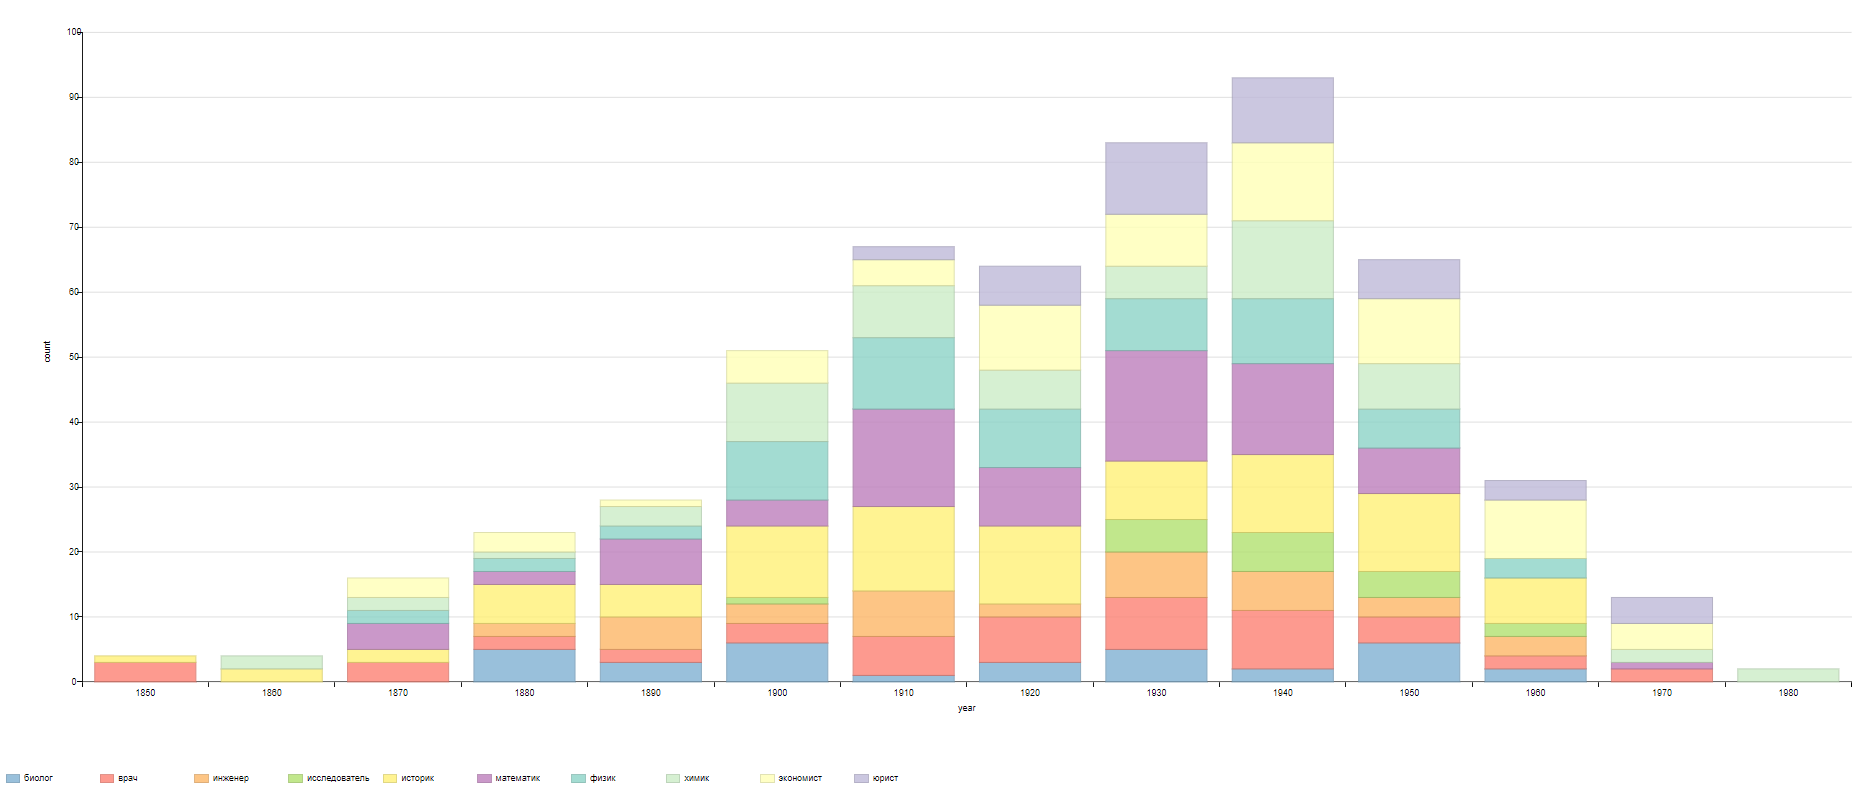
\includegraphics[width=1\linewidth]{./chapter/human_settlement/RussianScientistBornVillage.png}}
	\label{fig:human-settlement-5}
	\caption[Диаграмма количества ученых по родам деятельности родившихся в сельских поселениях.]{Диаграмма количества ученых по родам деятельности родившихся в сельских поселениях. Ссылка на SPARQL-запрос: \href{https://w.wiki/xxxx}{https://w.wiki/xxxx}.}%
\end{figure*} 

%%%%%
\subsection{Построение диаграммы для учёных родившихся в городских поселениях и сравнение диаграмм}

Используя вышеописанные шаги, получаем такой результат (листинг ~\protect\ref{lst:human-settlement17}).

\index{SPARQL!COUNT!Диаграмма количества ученых по родам деятельности родившихся в городских поселениях}
\index{SPARQL!FILTER!Диаграмма количества ученых по родам деятельности родившихся в городских поселениях}
\index{SPARQL!FLOOR!Диаграмма количества ученых по родам деятельности родившихся в городских поселениях}
\index{SPARQL!YEAR!Диаграмма количества ученых по родам деятельности родившихся в городских поселениях}
\index{SPARQL!STR!Диаграмма количества ученых по родам деятельности родившихся в городских поселениях}
\index{SPARQL!BIND!Диаграмма количества ученых по родам деятельности родившихся в городских поселениях}
\index{SPARQL!GROUP BY!Диаграмма количества ученых по родам деятельности родившихся в городских поселениях}
\index{График!BarChart!Диаграмма количества ученых по родам деятельности родившихся в городских поселениях}

\begin{lstlisting}[ language=SPARQL, 
                    caption={\href{https://w.wiki/xxxx}{Диаграмма количества ученых по родам деятельности родившихся в городских поселениях}\protect\footnotemark},
                    label=lst:human-settlement17,
                    texcl 
                    ]
# defaultView:BarChart
# Diagram of the number of scientists by occupation in town settlements

\end{lstlisting}%
\footnotetext{Ссылка на SPARQL-запрос: \href{https://w.wiki/xxxx}{https://w.wiki/xxxx}}

Диаграмма ~\ref{fig:human-settlement-6} показывает количество ученых по родам деятельности родившихся в городских полесениях.

\begin{figure*}
    \setlength{\fboxsep}{0pt}%
    \setlength{\fboxrule}{1pt}%
    \fcolorbox{gray}{gray}{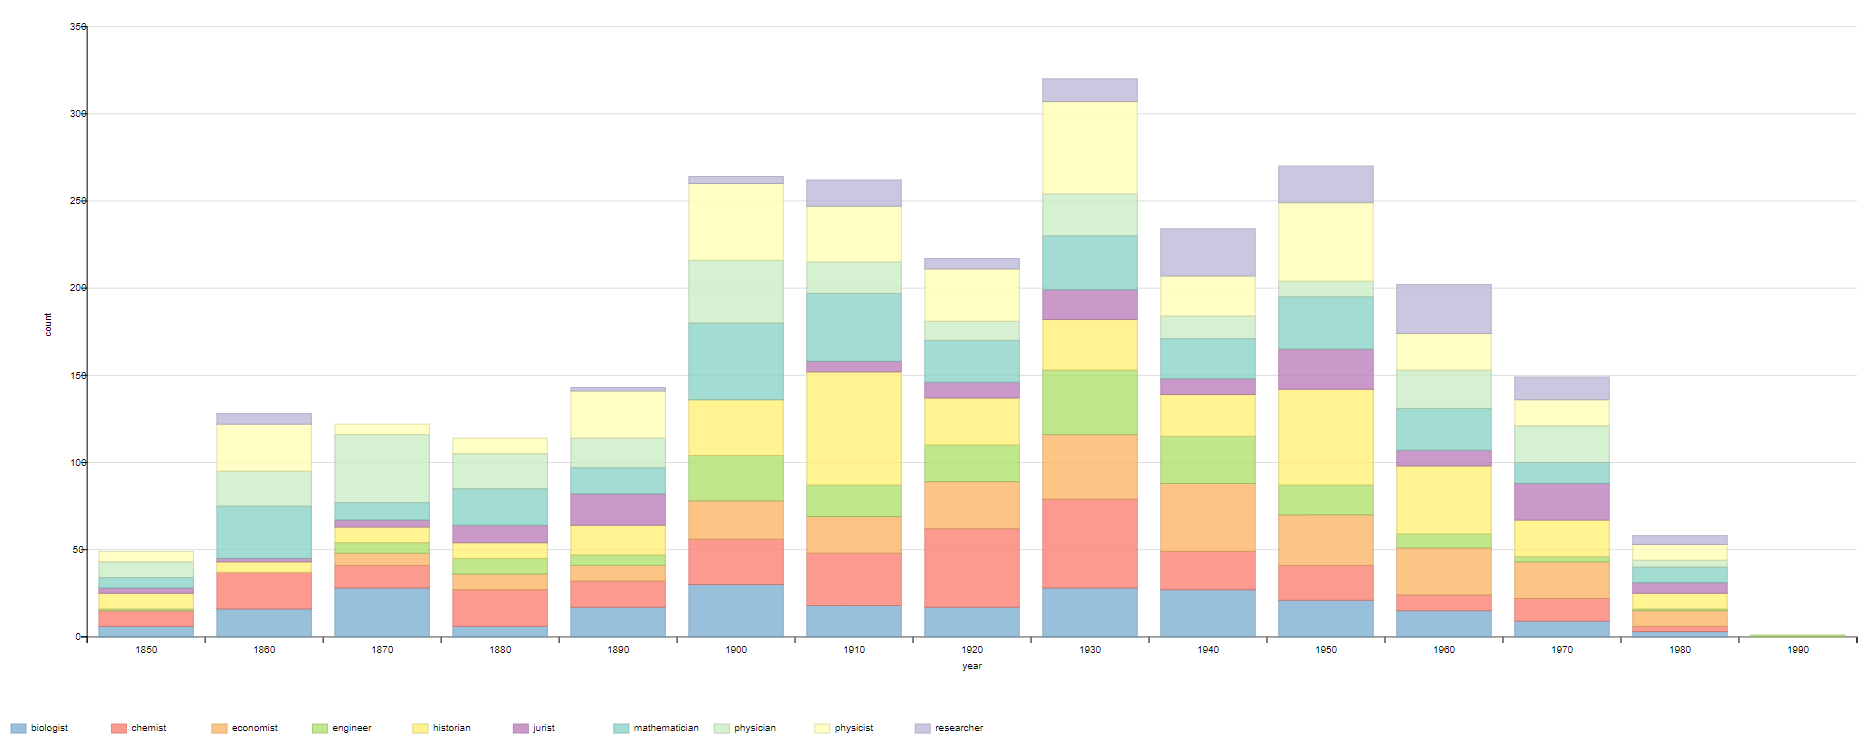
\includegraphics[width=1\linewidth]{./chapter/human_settlement/RussianScientistBornTown.png}}
	\label{fig:human-settlement-6}
	\caption[Диаграмма количества ученых по родам деятельности родившихся в городских поселениях.]{Диаграмма количества ученых по родам деятельности родившихся в городских поселениях. Ссылка на SPARQL-запрос: \href{https://w.wiki/xxxx}{https://w.wiki/xxxx}}%
\end{figure*} 

Сравнив диаграммы, видно что ученных в городских поселениях больше примерно в 3 раза, чем в сельских поселениях. Выше мы считали количество населения с этих группах, разница в населении достигает почти в 4 раза. Следовательно можно сказать, что не важно где ты родился. 

\setchapterimage[6cm]{chapter/operating_system/logo.png}
\setchapterpreamble[u]{\margintoc}
\chapter[line 1 line 2]{Programming languages for operating systems}
\labch{operating-sysmets}

\section{Annotation}
The chapter explores the object of the <<operating system>> and its properties. The following problems were solved in the paper with the help of SPARQL queries: finding instances of the object <<operating system>>, building a list of operating systems (OS) by base, by creation time, by programming language, in which the OS was written. Also a histogram is constructed, it shows the number of programs written in some programming language, and the proportion of how many of them work for some OS. A lot of software does not specify the programming language on which it was developed. The property <<programming language>> was added to several objects to improve the results.

\section{Instances of the object "operating system"}

Let's build a list of all the operating systems.

\begin{lstlisting}[ language=SPARQL, 
caption={List of operating systems\\\hspace{\textwidth} 
SPARQL query \num{510} results (January 2018), \num{1086} results (September 2020).
SPARQL query: \href{https://w.wiki/nDb}{https://w.wiki/nDb}
},
label=lst:os-list,
texcl 
]
#List of `instances of` "operating system" 
SELECT ?os ?osLabel
WHERE
{
	?os wdt:P31 wd:Q9135.
	SERVICE wikibase:label { bd:serviceParam wikibase:language "en" }
}
}
\end{lstlisting}

[+]> The most complete and detailed operating systems on Wikidata are: Linux, Windows, Windows 8

[-]> Almost empty and less informative operating systems are: SPIN, JavaOS, Atari TOS, Xubuntu

According to ProWD the only one Russian operating system on Wikidata is Miraculix, which has 7 properties. The leaders in terms of the number of properties (24 properties) among operating systems around the world are Microsoft Windows and Windows 8.

\section{List of operating systems by base}

\begin{lstlisting}[ language=SPARQL, 
caption={List of operating systems by base\\\hspace{\textwidth}
SPARQL query \num{159} results (January 2018), \num{118} results (September 2020).
SPARQL query: \href{https://w.wiki/nDc}{https://w.wiki/nDc}
},
label=lst:os-by-base,
texcl 
]
SELECT ?osLabel ?baseLabel
WHERE
{
	?os wdt:P31 wd:Q9135. # inctance of operating system
	?os wdt:P144 ?base. # os is base for 
	SERVICE wikibase:label { bd:serviceParam wikibase:language "en" }
}
GROUP BY ?osLabel ?baseLabel
\end{lstlisting}

\section{List of operating systems by creation time}


\begin{lstlisting}[ language=SPARQL, 
caption={List of operating systems by creation time\\\hspace{\textwidth}
SPARQL query \num{298} results (January 2018), \num{238} results (September 2020).
SPARQL query: \href{https://w.wiki/nDf}{https://w.wiki/nDf}
},
label=lst:os-creation-time,
texcl 
]
#defaultView:Timeline
SELECT ?osLabel ?time
WHERE
{
	?os wdt:P31 wd:Q9135. # inctance of operating system
	?os wdt:P571 ?time. # created at
	SERVICE wikibase:label { bd:serviceParam wikibase:language "en" }
}
GROUP BY ?osLabel ?time
ORDER BY DESC(?time)
\end{lstlisting}

\section{Count of operating systems by programming language}

\begin{lstlisting}[ language=SPARQL, 
caption={Count of operating systems by programming language\\\hspace{\textwidth}
SPARQL query \num{35} results (January 2018), \num{37} results (September 2020).
SPARQL query: \href{https://w.wiki/nDh}{https://w.wiki/nDh}
},
label=lst:prog-lang-count,
texcl 
]
#defaultView:BarChart
SELECT ?lang (count(*) as ?count)
WHERE 
{
	?os wdt:P31 wd:Q9135.
	?os wdt:P277 ?langObj .
	OPTIONAL {
		?langObj rdfs:label ?lang
		filter (lang(?lang) = "en")
	}
}
GROUP BY ?lang
ORDER BY DESC(?count) ASC(?lang)
\end{lstlisting}

The query shows (only on the basis of the completed wikis, so it's not a fact that it's true) that the OS is predominantly written in Assembler language, which is certainly true, because it is the fastest, yet convenient programming language. On the second and third places are C and C++, which are not the worst analogue, because in spite of its "slowness", they are the most convenient and simple programming languages.

\subsection{The programming languages used to write the operating system}

It is also interesting to look at the results of this query in the form of a graph, it is also perfectly visible on it how many objects simply have an empty field "programming language".

\begin{lstlisting}[ language=SPARQL, 
caption={The programming languages used to write the operating system\\\hspace{\textwidth}
SPARQL query \num{533} results (March 2017), \num{1117} results (September 2020)
SPARQL query: \href{https://w.wiki/eLH}{https://w.wiki/eLH}
},
label=lst:lang-used-to-os,
texcl 
]
#defaultView:BarChart
SELECT ?lang (count(*) as ?count)
WHERE 
{
	?os wdt:P31 wd:Q9135.
	?os wdt:P277 ?langObj .
	OPTIONAL {
		?langObj rdfs:label ?lang
		filter (lang(?lang) = "en")
	}
}
GROUP BY ?lang
ORDER BY DESC(?count) ASC(?lang)
\end{lstlisting}

If you look at the same query, but with such a restriction that at least the number of operating systems written in the language is at least 2, you can see a significant difference with the result of the previous query.


\begin{lstlisting}[ language=SPARQL, 
caption={Graph of languages used to create operating systems\\\hspace{\textwidth}
SPARQL query \num{118} results (September 2020)
SPARQL query: \href{https://w.wiki/nDm}{https://w.wiki/nDm}
},
label=lst:graph-os-by-lang,
texcl 
]
#defaultView:Graph
SELECT ?os ?osLabel ?language ?languageLabel
WHERE
{
	{
		SELECT ?language ?languageLabel
		WHERE {
			?os wdt:P31 wd:Q9135. # os is os
			?os wdt:P277 ?language. # os written by language
			SERVICE wikibase:label { bd:serviceParam wikibase:language "en" }
		} 
		Group by ?language ?languageLabel 
		Having (Count(?os) > 1) # get laguages which has more than one written os
	}
	?os wdt:P31 wd:Q9135. # os is os
	?os wdt:P277 ?language. # os written by language
	SERVICE wikibase:label { bd:serviceParam wikibase:language "en" }
}
\end{lstlisting}
\setchapterpreamble[u]{\margintoc}
\chapter{Where do inventors of programming languages study and what are their profession}
\labch{programming_language}

\section{Abstract}
The article examines the properties of programming languages based on the knowledge base of the international project Wikidata. A number of problems have been solved with the help of SPARQL queries calculated on objects of the "programming language"\  type in Wikidata. Lists of all programming languages under permissive licenses and languages with closed licenses were obtained and their percentage was calculated. A bubble chart was built by the number of source code file formats. Maps have been received showing the location of educational institutions and companies in which people associated with the creation of programming languages studied or worked. A bubble diagram has been built showing the professions of people involved in the creation and development of programming languages. A list of all object-oriented programming languages was obtained and a conclusion was drawn about the exhaustive completeness of Wikidata regarding them. Comparison and analysis of the results of SPARQL queries of 2017 and 2020 are carried out, the main changes are noted.


\setchapterpreamble[u]{\margintoc}
\chapter{Ships and their operators}

\labch{ships}

\section{Abstract}

This chapter focuses on ships in Russia and the world. Ships may have different purposes: military, or civil. Civilian ships are used in a variety of tasks: trucking, fishing, tourism, mineral exploration, rescue work, as well as sports, cultural and other activities. To store a large amount of information about all ships, it is necessary to maintain knowledge bases. One of those knolange bases is Wikidata. This work is aimed at studying the stord in Wikidata objects describing ships and at evaluating the quality and completeness of their properties and descriptions.


\section{Instances of the object "ship"}


\begin{lstlisting}[ language=SPARQL, caption={{List of ship in English}\protect\footnotemark}, label=lst:list_of_ship_en, ]
    SELECT ?ship ?shipLabel
    WHERE
    {
      ?ship wdt:P31 wd:Q11446. # instance of ship
      SERVICE wikibase:label { bd:serviceParam wikibase:language "en". }
    }
  \end{lstlisting}
  \footnotetext{\href{https://w.wiki/nDi}{SPARQL-query}, \num{19820}results (2017), \num{50681} results (2020).}

  
\begin{lstlisting}[ language=SPARQL, caption={{List of ship from Russia, Soviet Union and Russian Empire}\protect\footnotemark}, label=lst:list_of_ship_ussr_rf_re_en, ]
    SELECT ?ship ?shipLabel
    WHERE
    {
      ?ship wdt:P31 wd:Q11446. # instance of ship
                                         # ships belongs to:
      { ?ship wdt:P137/wdt:P17 wd:Q34266 } UNION  # Russian Empire
      { ?ship wdt:P137/wdt:P17 wd:Q15180 } UNION  # Soviet Union
      { ?ship wdt:P137/wdt:P17 wd:Q159 }.         # Russia
      SERVICE wikibase:label { bd:serviceParam wikibase:language "en". }
    }
  \end{lstlisting}
  \footnotetext{\href{https://w.wiki/nDk}{SPARQL-query}, \num{107}results (2017), \num{579} results (2020).}

    
\section{Filling the properties of warships}
\begin{lstlisting}[ language=SPARQL, caption={{List of ships with countries and war conflicts in English}\protect\footnotemark}, label=lst:ships_in_conflict_en, ]
    SELECT ?ship ?shipLabel ?countryLabel ?conflict ?conflictLabel
    WHERE
    {
      ?ship wdt:P31 wd:Q11446;        # instance of ship
            wdt:P137/wdt:P17 ?country;         # belongs to country
            wdt:P607 ?conflict.       # engaged in some conflict
      SERVICE wikibase:label { bd:serviceParam wikibase:language "en". }
    }
  \end{lstlisting}
  \footnotetext{\href{https://w.wiki/nDo}{SPARQL-query}, \num{1400}results (2017), \num{3586} results (2020).}

  \begin{lstlisting}[ language=SPARQL, caption={{List of ship with countries and war conflicts in English}\protect\footnotemark}, label=lst:ships_in_conflict_2_en, ]
    SELECT ?ship ?shipLabel ?countryLabel ?conflict ?conflictLabel
    WHERE
    {
      ?ship wdt:P31 wd:Q11446;        # instance of ship
            wdt:P137/wdt:P17 ?country;        # belongs to operator
            wdt:P607 ?conflict.       # engaged in some conflict
      
      { ?country wdt:P17 wd:Q34266 } UNION  # Russian Empire
      { ?country wdt:P17 wd:Q15180 } UNION  # Soviet Union
      { ?country wdt:P17 wd:Q159 }.         # Russia
      
      SERVICE wikibase:label { bd:serviceParam wikibase:language "en". }
    }
  \end{lstlisting}
  \footnotetext{\href{https://w.wiki/nDn}{SPARQL-query}, \num{105}results (2017), \num{86} results (2020).}
\setchapterimage[6cm]{chapter/spacecraft/Takhir-Salakhov-For-You-Humanity-1961-2011-title-moved.jpg}

\setchapterpreamble[u]{\margintoc}
\chapter{Spacecraft and space stations}
\labch{spacecraft}
\footnotetext{Painting by Takhir Salakhov ``For You, Humanity!'' (1961), reproduced on the stamp of Azerbaijan in 2011 on the 50th anniversary of First Manned Space Flight (the flight of Yuri Gagarin). 
\href{https://commons.wikimedia.org/wiki/File:Stamps\_of\_Azerbaijan,\_2011-944.jpg}{Wikimedia Commons}.}

The chapter is devoted to research of spaceships and stations based on Wikidata. 
Using SPARQL scripts, a list of Russian ships and stations is constructed, 
a timeline of the launching of ships in our country and in the world for the period from 1960 to 2021 is drawn. 
An evaluation of the completeness of Wikidata was performed, showing, 
that many of the items have the wrong value of the property 
\wdProperty{31}{instance of}. In the course of the work, it was found that the current performance of Russian astronautics in terms of the number of spacecraft launches in recent years matches that of the USSR fifty years ago. 

\section{List of space ships and stations}
Let's build a query~\ref{lst:spaceships} to output a list of all spaceships and stations. 
We need the objects \wdqName{space station}{25956}, 
\wdqName{spacecraft}{40218} and the relation \wdProperty{31}{instance of}. 

\index{SPARQL!VALUES!List of space ships and stations}
\index{SPARQL!SERVICE!List of space ships and stations}
\begin{lstlisting}[ language=SPARQL, breaklines=true, numbers=none,%
                    caption={Retrieves list of all spaceships and stations. The result contained \num{145} objects in 2021. SPARQL query: \href{https://w.wiki/4eeL}{https://w.wiki/4eeL}},%
                    label=lst:spaceships,%
                    texcl%
                    ]
# List of spacecraft (Q40218) and space station (Q25956)
SELECT  ?s ?sLabel ?typeLabel
WHERE
{
  VALUES ?type {wd:Q40218 wd:Q25956}
  ?s wdt:P31 ?type.  # Selecting the type of object
  SERVICE wikibase:label {bd:serviceParam wikibase:language"en"}
}
\end{lstlisting}%

\begin{marginfigure}
{
	\setlength{\fboxsep}{0pt}%
	\setlength{\fboxrule}{1pt}%
	\fcolorbox{gray}{gray}{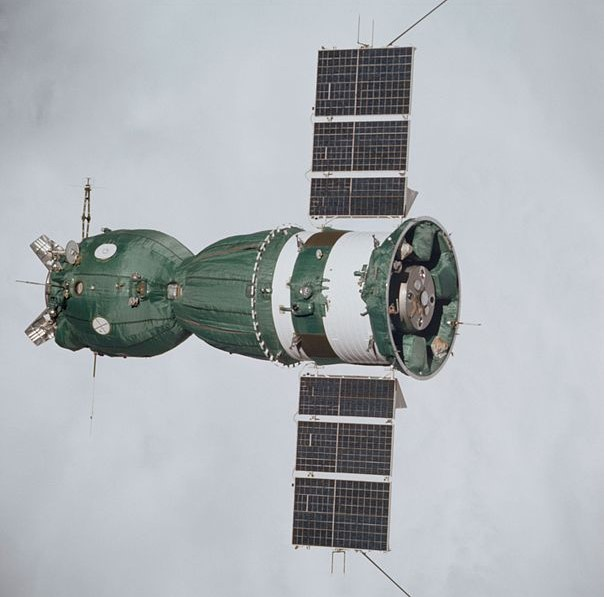
\includegraphics{graphics/chapter/spacecraft/soyuz-19.jpg}}
}
\caption[Soyuz-19.]%
{In which country is the machine shown in the picture designed?
See the answer~\ref{answer:spacecraft_USSR} on the p.~\pageref{answer:spacecraft_USSR}.}
\label{question:spacecraft_soyuz19}
\end{marginfigure}

\section{Depth of object development}

As of 2021 on Wikidata \wdqName{Apollo-8}{184201} {wdqName} is the most complete and elaborate spacecraft, which has 30 properties.\autocite{spacecraftProWD} At the same time, only one property each has ships such as: \wdqName{Europa Astrobiology Lander}{10491365}, \wdqName{Project Orbiter}{6514453}, \wdqName{LRK}{5961734}, \wdqName{EarthForce One}{5327028}%
\sidenote[][]{%
Note the difficult fate of the object \wdqName{EarthForce One}{5327028}. This object was automatically created in Wikidata by a bot in 2013, because there was an English Wikipedia article. According to the ``\href{https://en.wikipedia.org/wiki/EarthForce_One}{EarthForce One}`` English Wikipedia, the article was removed due to a lack of reliable sources proving the significance of the site. And the object has been left as an unremarkable item on Wikidata. Think of a query that would output a list of similar Wikidata items, that does not match any Wikipedia article.%
},%
\wdqName{Souyz GVC}{60767924}, %
\wdqName{CubeSat for Solar Particles}{22907583}.\autocite{spacecraftProWD} %
To find this information, a query built with the ProWD\autocite{spacecraftProWD} service was used. %
The same service showed that the number of properties of space objects is uneven, %
most are less than 30\% filled.\autocite{spacecraftProWD} %

\section{List of Soviet and Russian spaceships and stations}

Let us find ships and stations designed in USSR or Russia, using the query~\ref{lst:spaceshipsUSSR}.

\index{SPARQL!VALUES!List of Soviet and Russian spaceships and stations}
\index{SPARQL!SERVICE!List of Soviet and Russian spaceships and stations}
\begin{lstlisting}[ language=SPARQL, breaklines=true, numbers=none,%
                    caption={Retrieves list of Soviet and Russian spaceships and stations. \num{3} results in 2017 and \num{25} results in 2021. SPARQL query: \href{https://w.wiki/4eeR}{https://w.wiki/4eeR}},%
                    label=lst:spaceshipsUSSR,%
                    texcl%
                    ]
# List of Russian and USSR spacecrafts and stations
SELECT  ?spacecraft  ?spacecraftLabel 
WHERE
{
  {?spacecraft wdt:P31 wd:Q40218.} UNION #spacecraft
  {?spacecraft wdt:P31 wd:Q25956.} # and space station
  
  # Soviet Union and Russia
  VALUES ?ruCountries {wd:Q15180 wd:Q159}
  ?spacecraft wdt:P17 ?ruCountries. # related to Russia
  
  SERVICE wikibase:label {bd:serviceParam wikibase:language "en"}
}
\end{lstlisting}%

\begin{marginfigure}
{
	\setlength{\fboxsep}{0pt}%
	\setlength{\fboxrule}{1pt}%
	\fcolorbox{gray}{gray}{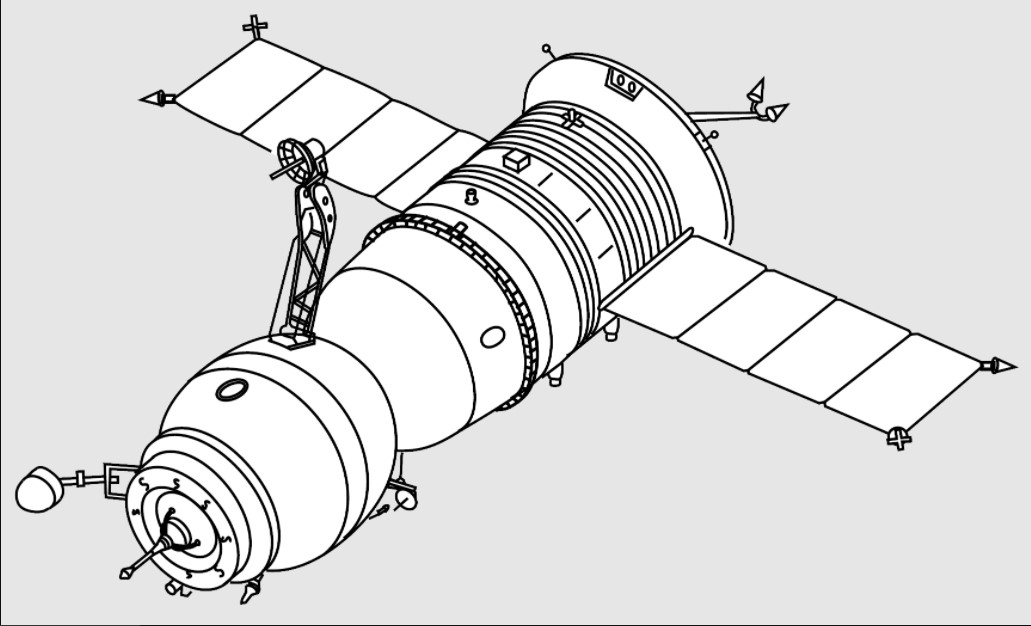
\includegraphics{graphics/chapter/spacecraft/soyuz-t.jpg}}
}
\caption
[Soyuz-T.]{%
In which country is the machine shown in the picture designed?

See the answer~\ref{answer:spacecraft_USSR} on the p.~\pageref{answer:spacecraft_USSR}.
}
\label{question:spacecraft_soyuzT}
\end{marginfigure}

\section{Analyzing the Completeness of Wikidata}

Let us analyze the degree of filling in Wikidata in the field of Soviet and Russian spaceships and stations.
By Query~\ref{lst:spaceships} 145 results were obtained for all ships and stations,
by Query~\ref{lst:spaceshipsUSSR} about Soviet and Russian objects~--- only 25.
Information about~Soviet and Russian objects in 2021
has become several times more compared to 2017,
when on Query~\ref{lst:spaceshipsUSSR} only 3 objects were returned.

As of 2021, the Buran.ru website in the section about the spaceships of the USSR and Russia contains information about 36 ships.\autocite{spacecraftBuran} %
There are 51 launches of spaceships from 1957 to 1984 in Soviet Union and 43 in same years in the United States.\autocite[480-483]{spacecraftCosmonavtika} This means that less than half of the Soviet spaceships are represented in Wikidata.
There are 10 Soviet and Russian launches of space stations\autocite[296]{spacecraftSAA},
126 NASA shuttle launches from 1981 to 2008\autocite[288]{spacecraftSAA}
and 31 international launch vehicles\autocite[290-291]{spacecraftSAA} in the American directory of space and astronomy.

\section{Time schedules of space exploration in Russia (include USSR) and the World}

Spacecraft launch schedule in Russia since 1960s (Figure~\ref{fig:launchesRussia5years})
built with Query~\ref{lst:launchesRussia5years}.%

Earlier, in queries to get any lists, we used the \wdProperty{31}{instance of} property.
The Query~\ref{lst:launchesRussia5years} without this property, with using the relation
\wdProperty{619}{<< spaceship launch date >>} on line 10
for traversing and counting such objects that have been launched into space.
%
%%%%%%%%%%%%%%%% Exercise 1 %%%%%%%%%%%%%%%% 
\label{question:spacecraft_1}%
\marginnote{%
How many ships were launched in the~USSR in the~1960s, 1970s, and 1980s? %
See answer~\ref{answer:launches_USSR} on p.~\pageref{answer:launches_USSR}.%
}%
%
The logical operator \lstinline|UNION| on lines 5-8 in Query~\ref{lst:launchesRussia5years}
allows you to combine Soviet and Russian spacecraft launches.

If in the Query~\ref{lst:launchesRussia5years} instead of the variable \lstinline|?Lapse|~---\lstinline|?year| remained (lines 3 and 12),
then we would get in Figure~\ref{fig:launchesRussia5years}
the number of launches each year.
Thanks to the rounding function \lstinline|FLOOR()|
and grouping%
\sidenote[][8.0cm]{
%
On line 14 of the query,~\ref{lst:launchesRussia5years}
objects launched into space are grouped by the command:
\mbox {\lstinline|GROUP BY ?lapse|.} \newline
The fact that the grouping goes exactly according to five-year range, and not, for example, six-year-olds,
is defined on line 12, where the \lstinline|?year| divided by 5, rounded, and multiplied by 5.%
%
},
\lstinline|?item| objects that have launches are grouped over a five-year period,
and into the variable \lstinline|?quantity| the number of these objects is recorded,
calculated using the \lstinline|COUNT()| function.

The BarChart command in Query~\ref{lst:launchesRussia5years} is used to present the results as a bar chart in Figure~\ref{fig:launchesRussia5years}.

\index{SPARQL!STR!Schedule of spacecraft launches in the USSR and Russia (by five years)}
\index{SPARQL!COUNT!Schedule of spacecraft launches in the USSR and Russia (by five years)}
\index{SPARQL!UNION!Schedule of spacecraft launches in the USSR and Russia (by five years)}
\index{SPARQL!BarChart!Schedule of spacecraft launches in the USSR and Russia (by five years)}
\index{SPARQL!GROUP BY!Schedule of spacecraft launches in the USSR and Russia (by five years)}
\index{SPARQL!ORDER BY!Schedule of spacecraft launches in the USSR and Russia (by five years)}
\index{SPARQL!BIND!Schedule of spacecraft launches in the USSR and Russia (by five years)}
\index{SPARQL!FLOOR!Schedule of spacecraft launches in the USSR and Russia (by five years)}
\begin{lstlisting}[ language=SPARQL, breaklines=true, %
                    caption={Draw schedule of spacecraft launches in the USSR and Russia (by five years). Found \num{14} five-year range in 2021. SPARQL query: \href{https://w.wiki/4f7Y}{https://w.wiki/4f7Y}},%
                    label=lst:launchesRussia5years,%
                    texcl%
                    ]
# The number of spacecraft launches in Russia every 5 years
#defaultView:BarChart
SELECT (STR(?lapse) AS ?lapse_str) (COUNT(?item) AS ?quantity)
WHERE {                                  # spacecraft belongs to
        {?item wdt:P17 wd:Q15180}               # country = USSR
  UNION {?item wdt:P17 wd:Q159}               # country = Russia
  UNION {?item wdt:P495 wd:Q159}    # country of origin = Russia
  UNION {?item wdt:P495 wd:Q15180}.  # country of origin =  USSR
  
  ?item wdt:P619 ?launch. # date of spacecraft launch
  BIND( YEAR(?launch) AS ?year) 
  BIND(FLOOR(?year/5)*5 AS ?lapse) # count for each 5 years
} 
GROUP BY ?lapse
ORDER BY ?lapse # Order 1970, 1975, 1980, ...
\end{lstlisting}%

\index{Graph!Diagram!Schedule of spacecraft launches in the USSR and Russia (by five years)}
\begin{figure*}[h!]
  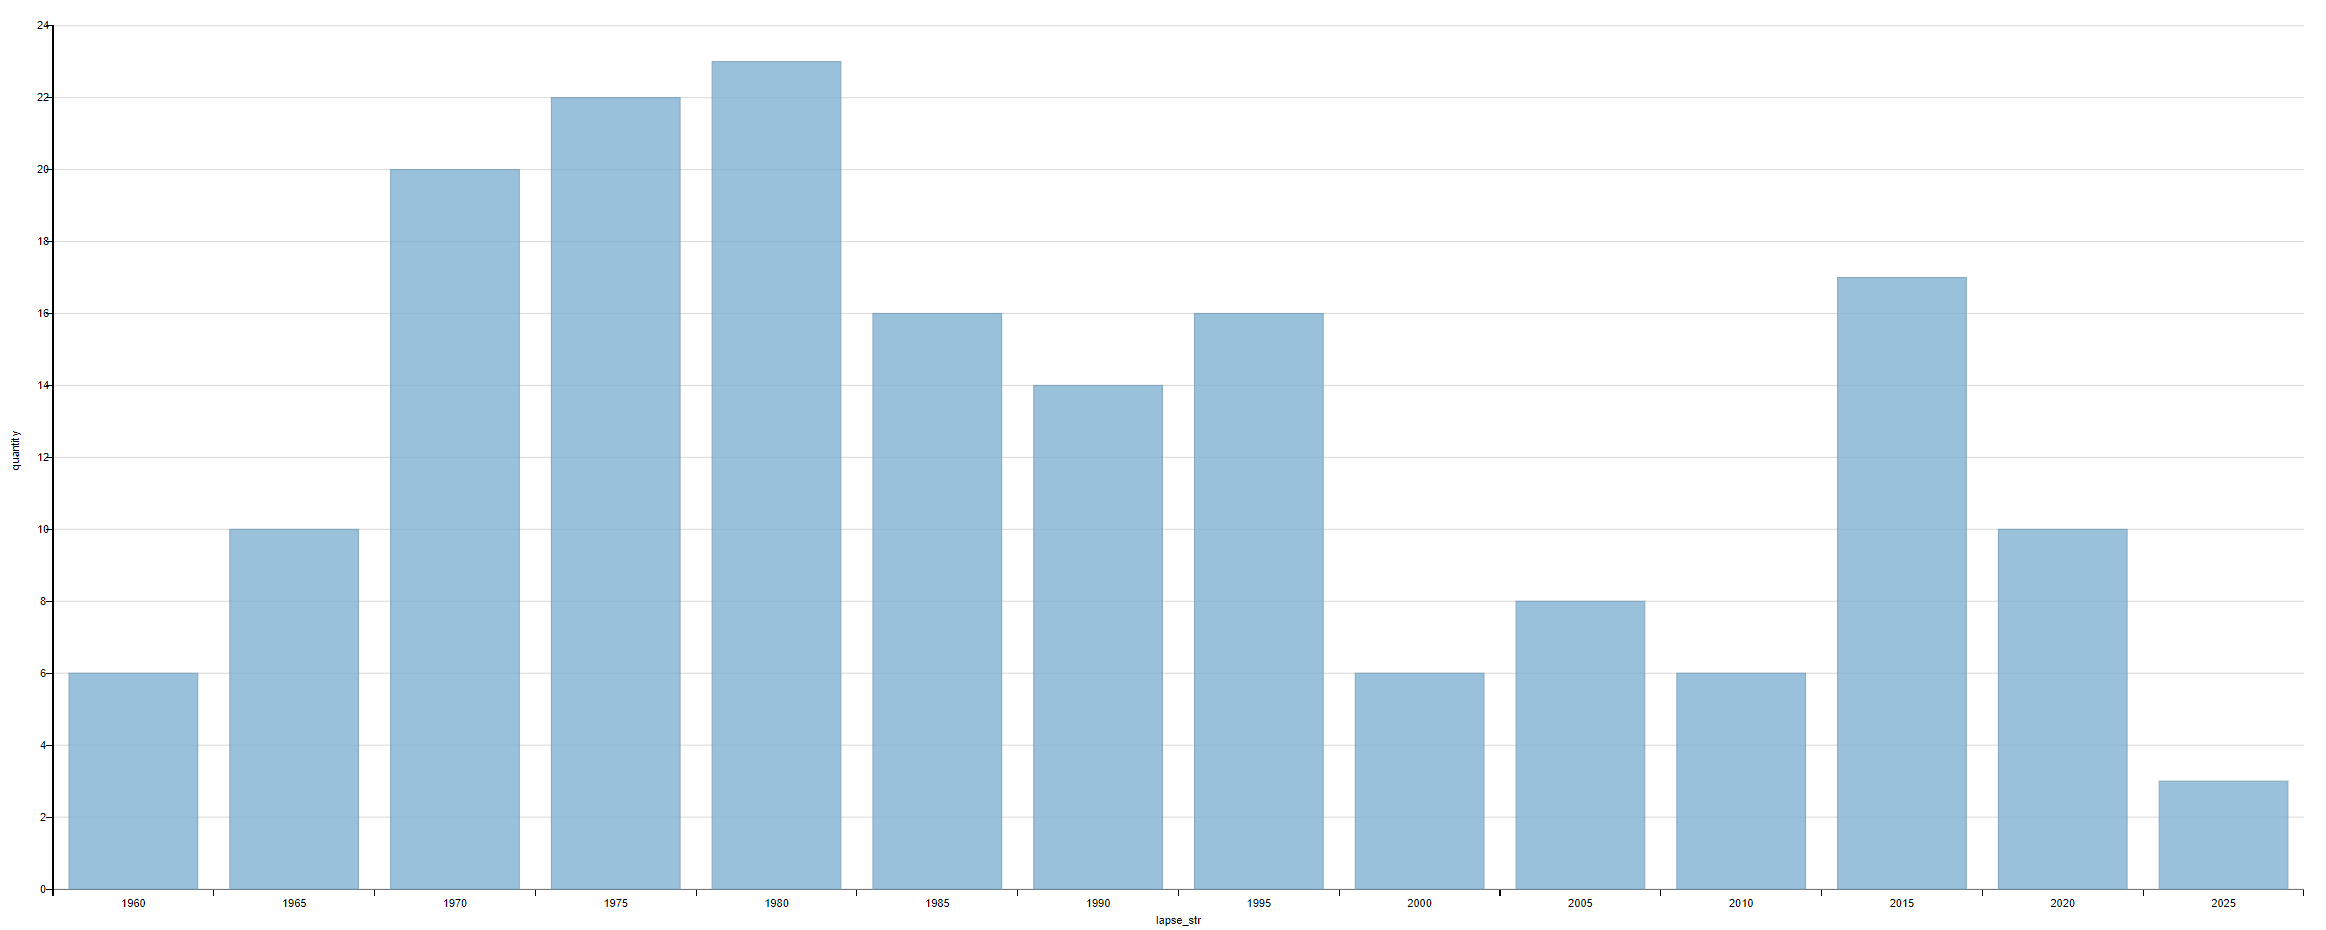
\includegraphics[width=\linewidth]{graphics/chapter/spacecraft/Visualization of the number of spacecraft launches in USSR and Russia per 5 years 2022.png}
  \caption[Schedule of spacecraft launches in the USSR and Russia (by five years)] {Visualization of the number of spacecraft launches in the USSR and Russia every 5 years, built with Query~\protect\ref{lst:launchesRussia5years}, 2022.}%
  \label{fig:launchesRussia5years}%
\end{figure*}

The horizontal axis in Figure~\ref{fig:launchesRussia5years} is answered by the variable \mbox{\lstinline|?lapse_str|}. 
If you don't convert the number \lstinline|?lapse| 
into a text variable \mbox{\lstinline|?lapse_str|}%
\sidenote[][]{
%
Converting a number into text  
in the third line of the query~\ref{lst:launchesRussia5years}:\newline
\lstinline|(STR(?lapse) AS ?lapse_str)|.%
%
}, then the~X axis has a range from 0 to 2200, 
instead of the required range from 1960 to 2025, 
and the results are indicated by points with coordinates (five years, number of launches), 
and the graph becomes unreadable. 

The Figure~\ref{fig:launchesRussia5years} shows, 
that the most active period of Russian cosmonautics development was in 1970--1995.

The Query~\ref{lst:launchesWorld} draws Figure~\ref{fig:launchesWorld} 
of spacecraft launches in the World by year and country.

\index{SPARQL!STR!Diagram of the number of spacecraft launches by year and country}
\index{SPARQL!BIND!Diagram of the number of spacecraft launches by year and country}
\index{SPARQL!COUNT!Diagram of the number of spacecraft launches by year and country}
\index{SPARQL!SERVICE!Diagram of the number of spacecraft launches by year and country}
\index{SPARQL!GROUP BY!Diagram of the number of spacecraft launches by year and country}
\index{SPARQL!YEAR!Diagram of the number of spacecraft launches by year and country}
\begin{lstlisting}[ language=SPARQL, breaklines=true, %
                    caption={Draws a diagram of the number of spacecraft launches by year and country. \num{328} results in 2021. SPARQL query: \href{https://w.wiki/4f8v}{https://w.wiki/4f8v}},%
                    label=lst:launchesWorld,%
                    texcl%
                    ]
# Diagram of spacecraft launches by year and country
#defaultView:BarChart
SELECT ?year (COUNT(?obj) AS ?count) ?country ?countryLabel
WHERE {
  ?obj wdt:P17 ?country. # spacecraft belongs to country 
  ?obj wdt:P619 ?launch. # date of spacecraft launch
  BIND(STR(YEAR(?launch)) AS ?year)
  
SERVICE wikibase:label {bd:serviceParam wikibase:language"en"}
}
GROUP BY ?year ?country ?countryLabel
\end{lstlisting}%

\index{Graph!Diagram!The schedule of spacecraft launches worldwide by year and country}
\begin{figure*}[h!]
  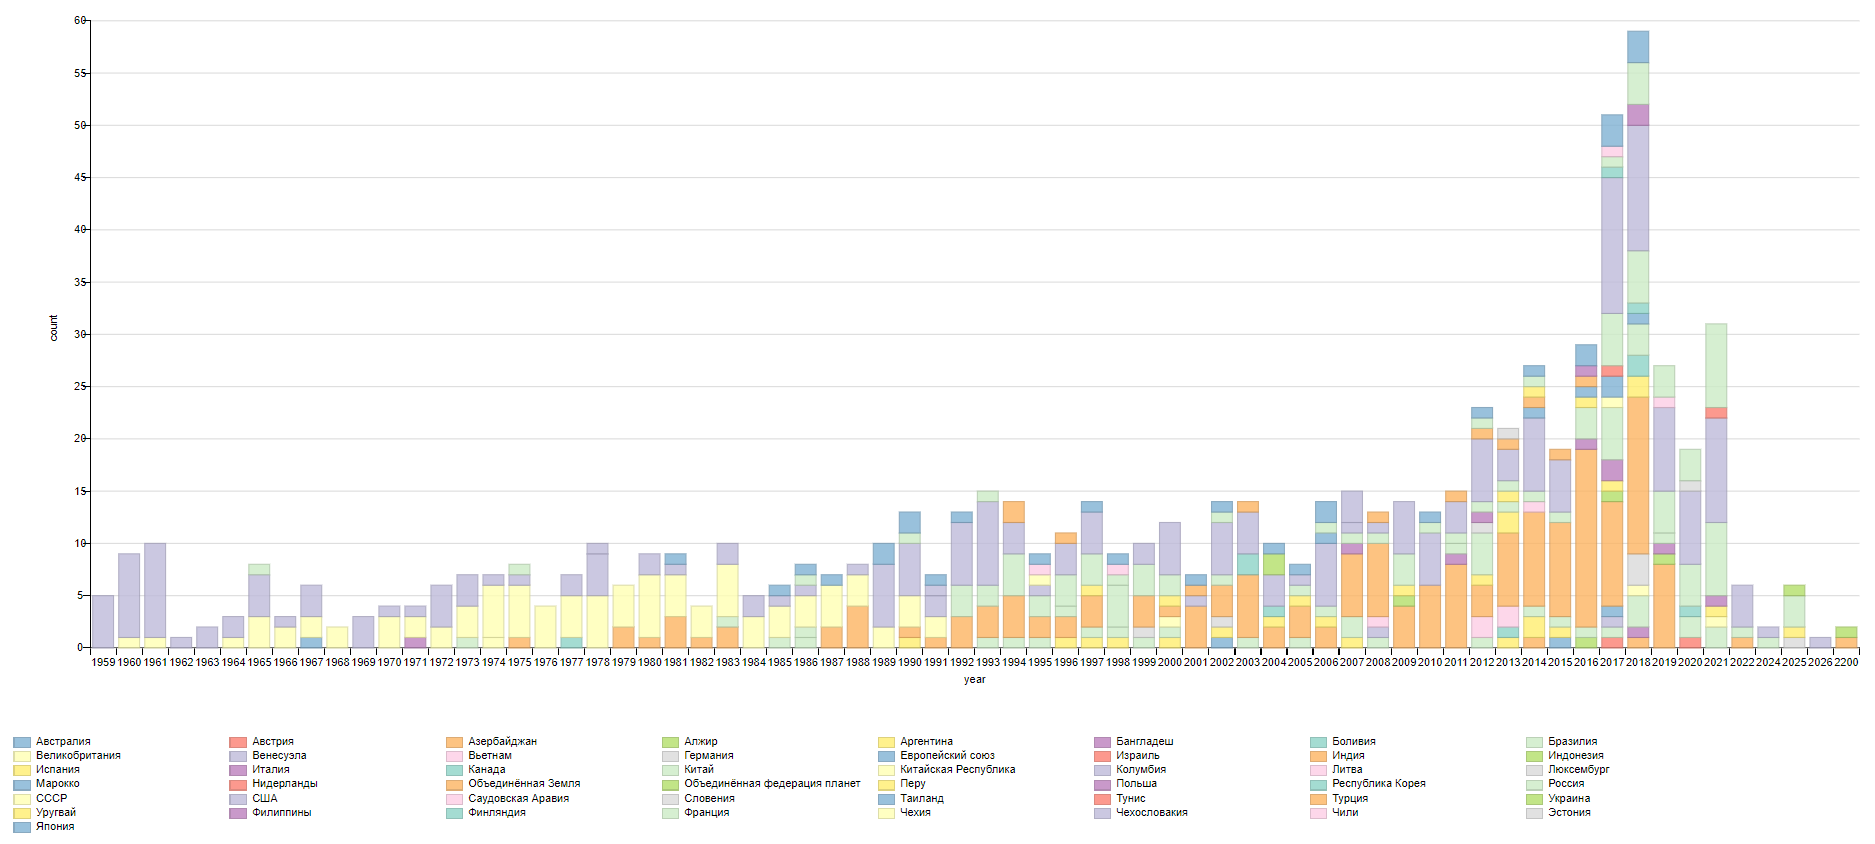
\includegraphics[width=\linewidth]{graphics/chapter/spacecraft/Visualization of the number of spacecraft launches by year and country 2021.png}
  \caption[The schedule of spacecraft launches worldwide by year and country]{Visualization of the number of spacecraft launches by year and country, built using a Query~\protect\ref{lst:launchesWorld} in 2021.}
  \label{fig:launchesWorld}%
\end{figure*}

Figure~\ref{fig:launchesWorld} shows that the most spacecraft 
launched by India and the United States. 
(only they launched more than 10 annual launches) in 2017--2018. 
Worldwide launches peaked in 2018 (59 launches). 

According to Wikidata, Russian cosmonautics ranks average in the number of launches, 
its numbers for 2016--2019 are similar to those of the USSR in the 1970s and 1980s 
and about 3--5 launches per year.

%%%%%%%%%%%%%%%% Exercise 2 %%%%%%%%%%%%%%%% 
\label{question:spacecraft_2}
\marginnote{%
What was the highest and lowest number of spacecraft launches humanity made in a decade between 1970 and 2010?
See answer~\ref{answer:max-min-space-launches} on p.~\pageref{answer:max-min-space-launches}.
}

\section{Astronauts in international flights}

Query~\ref{lst:internationalFlights} builds a graph~\ref{fig:internationalFlights} with vertices corresponding ``spaceships`` and ``astronaut``, colored by country.

\index{SPARQL!BIND!Draw the graph with the vertices of the type ``spaceships`` and ``astronauts`` with coloring by country.}
\index{SPARQL!SERVICE!Draw the graph with the vertices of the type ``spaceships`` and ``astronauts`` with coloring by country.}
\index{SPARQL!VALUES!Draw the graph with the vertices of the type ``spaceships`` and ``astronauts`` with coloring by country.}
\begin{lstlisting}[ language=SPARQL, breaklines=true, %
                    caption={Draw the graph with the vertices of the type ``spaceships`` and ``astronauts`` with coloring by country. The result contained \num{68} objects in 2022. SPARQL query: \href{https://clck.ru/agMjd}{https://clck.ru/agMjd}},%
                    label=lst:internationalFlights,%
                    texcl%
                    ]
# Graph of astronauts as crew of flights of different countries
#defaultView:Graph
SELECT DISTINCT ?item ?itemLabel ?rgb ?link ?naut_seed
WHERE
{ 
  VALUES ?toggle { true false }
  # Let's select a subset of astronauts
  {
    SELECT DISTINCT ?naut WHERE
    { 
      VALUES ?naut_seed {wd:Q313815}.  # Sergei Krikalev
      ?s wdt:P1029 ?naut_seed, ?naut;  
    }       # ?naut seed and ?naut are member of a same crew
  }
  ?s  wdt:P31/wdt:P279* wd:Q40218; # spacecraft
      wdt:P31/wdt:P279* wd:Q752783;# human spaceflight
          wdt:P1029 ?naut;  # has member of the crew ?naut    
  SERVICE wikibase:label {bd:serviceParam wikibase:language "en"}
  BIND(IF(?toggle,?s,?naut) AS ?item).
  BIND(IF(?toggle,?sLabel,?nautLabel) AS ?itemLabel).
  BIND(IF(?toggle,"FFFFFF","7FFF00") AS ?rgb_source).
  BIND(IF(?toggle,"",?s) AS ?link).
  ?naut wdt:P27 ?country. # astronaut is citizen of country 
  # ?toggle = true then spacecraft node
  # ?toggle = false then astronaut node
  BIND(     # Soviet and Russian astronauts have red nodes
    IF(!?toggle && (?country=wd:Q15180||?country=wd:Q159),"FF0000",
    IF(!?toggle && ?country=wd:Q30,"FF00FF",  # USA - fuchsia
    IF(!?toggle && ?country=wd:Q183,"C0C0C0", # Germany - silver
    IF(!?toggle && ?country=wd:Q142,"008080", # France - teal
    IF(!?toggle && ?country=wd:Q40,"800000", # Austria - maroon
    IF(!?toggle && ?country=wd:Q38,"00FFFF", # Italy - aqua
    ?rgb_source))))))
    AS ?rgb).
}
\end{lstlisting}%

\begin{marginfigure}
{
	\setlength{\fboxsep}{0pt}%
	\setlength{\fboxrule}{1pt}%
	\fcolorbox{gray}{gray}{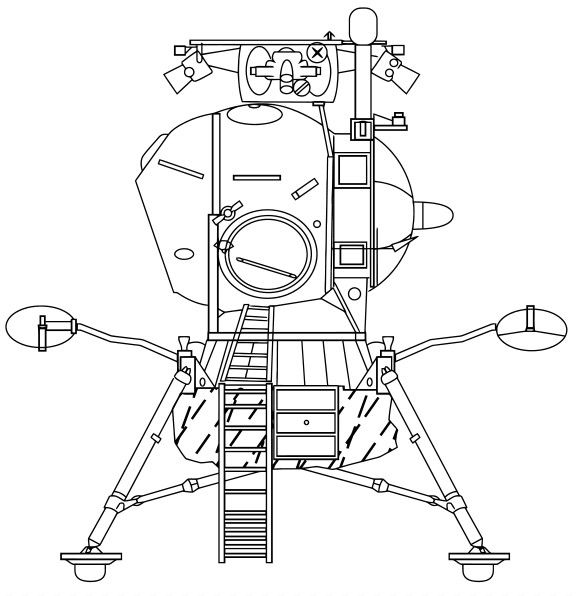
\includegraphics{graphics/chapter/spacecraft/lunar_landler.jpg}}
}
\caption[Lunar lander.]{%
In which country is the machine shown in the picture designed?

See the answer~\ref{answer:spacecraft_USSR} on the p.~\pageref{answer:spacecraft_USSR}.}
\label{question:spacecraft_lunar}
\end{marginfigure}

For the Query~\ref{lst:internationalFlights} to work, you must specify the starting point~--- an astronaut who has participated in the international spaceflight. The starting point is set at line 11 of the Query~\ref{lst:internationalFlights} and written to the \mbox{\lstinline|?naut_seed|} variable. Next, at line 12, we search for astronauts who have flown with the one we specified earlier. Lines 15--17 load data about spacecraft, flights and astronauts. Boolean variable \lstinline|?toggle| has value \lstinline|?true| if the found object is a spacecraft or \lstinline|?false| if the found object is an astronaut. The selected object (spacecraft or astronaut) is written to the \lstinline|?item| variable in line 19. In line 20 the name of the object is written to the variable \lstinline|?itemLabel|, in line 21 the data for the coloring of ships is written to the variable \mbox{\lstinline|?rgb_source|}. 

If a ship is selected, then nothing is written to the variable \lstinline|?link| in line 22. If an astronaut is selected, then his ship is written to the variable~\lstinline|?link|. On the graph this variable will correspond to the arc from the astronaut to the ship. 

Line 23 loads the astronaut's citizenship data, and~ lines 26--34 assign a color to the vertices of the astronauts in the graph, depending on their citizenship. 

\index{Graph!Graph!The graph with the vertices of the type ``spaceships`` and ``astronauts`` with coloring by country}
\begin{figure*}[h]
  \setlength{\fboxsep}{0pt}%
  \setlength{\fboxrule}{1pt}%
  \fcolorbox{gray}{gray}{%
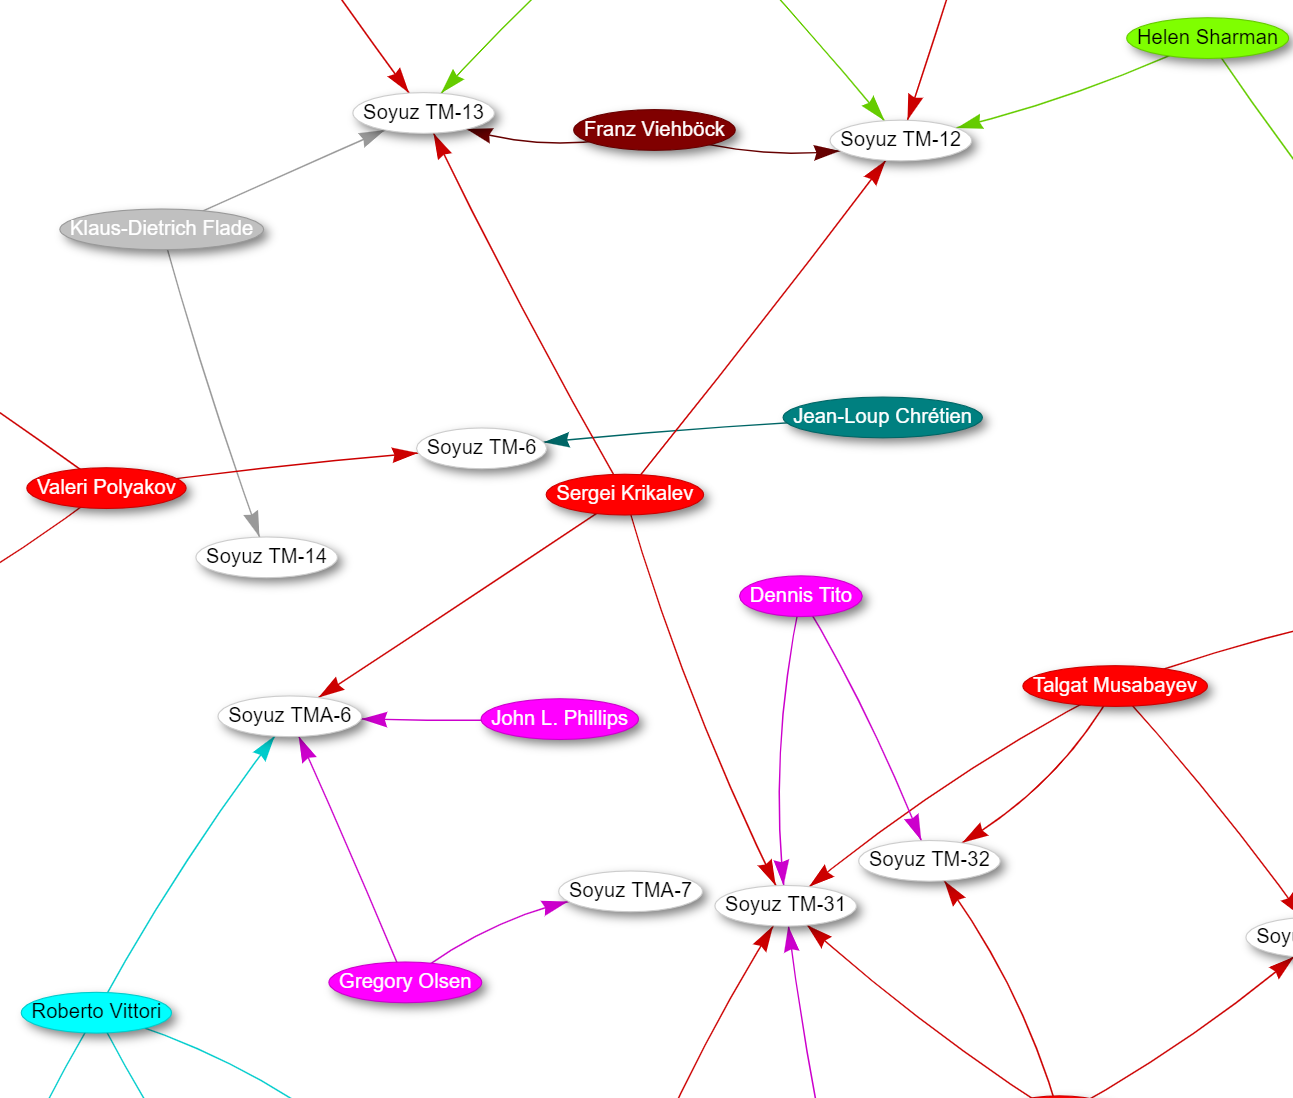
\includegraphics[width=\linewidth]{graphics/chapter/spacecraft/Cosmonauts in international flights EN.png}}
  \caption[The graph with the vertices of the type ``spaceships`` and ``astronauts`` with coloring by country]{The graph with the vertices of the type ``spaceships`` and ``astronauts`` with coloring by country. Red corresponds to the USSR and Russia, fuchsia~--- the USA, silver~--- Germany, teal~--- France, maroon~--- Australia, and aqua~--- Italy. The graph is built with the Query~\protect\ref{lst:internationalFlights}, 2022.}
  \label{fig:internationalFlights}%
\end{figure*}

\section{Exercises}
\begin{enumerate}
  \item Construct a list of ships that reached or will go to \wdqName{Mars}{111}.
  \item Calculate the proportion of ships (draw a graph by decade) which were sent 
        sent to \wdqName{Mars}{111} 
        in relation to the number of ships sent to \wdqName{Moon}{405}.
  \item Count the number of \wdqName{successful}{7632586} space launches 
      vis-a-vis \wdqName{failure}{1121708}\sidenote[][-32pt]{%
%
For example, the object \wdqName{<<Luna programme>>}{192372} 
the property \wdProperty{793}{<<significant event>>} 
specifies the number of successful and unsuccessful launches.%
}.%
\end{enumerate}

\chapter{Регионы России}
\label{ch:oblast-of-Russia}
Эта глава книги посвящена исследованию в Викиданных регионов России. 
Отметим, что регионы России включают в себя множество земель разного 
типа: области, республики, края и другие. Именно эти разнотипные регионы 
и были исследованы. Был построен граф субъектов России, граничащих 
с зарубежными странами (граф соседей), а также нарисована карта, 
на которой отмечена численность населения отдельных регионов. Оценка 
степени заполненности свойства Викиданных <<граничит с>> (shares border with) 
показала, что у каждого субъекта России эти данные заполнены полностью. 
Читатель познакомится с компьютерной обработкой Викиданных и визуализацией 
информации о регионах России.

\label{question:q_subjects_of_Russia_3}
\marginnote{О флаге какого субъекта идет речь:
<<Флаг этого субъекта представляет собой прямоугольное полотнище с отношением ширины к длине 2:3, красного цвета с двусторонним изображением в верхнем ближнем к древку углу основного элемента герба этого субъекта — развёрнутого к древку Святого \href{https://ru.wikipedia.org/wiki/Георгий_Победоносец}{Георгия Победоносца}. См. ответ \ref{answer:subjects_of_Russia_3} на с.~\pageref{answer:subjects_of_Russia_3}.}

\section{Экземпляры объекта <<Области России>>}

Для построения списка всех областей России нам потребуются объект 
\wdqName{<<области России>>}{835714} и свойство \wdProperty{31}{<<экземпляры>>} 
(листинг~\protect\ref{lst:oblast-of-Russia}).

\begin{lstlisting}[ language=SPARQL, 
                    caption={\href{https://w.wiki/4D2V}{Список всех областей России}\protect\footnotemark},
                    label=lst:oblast-of-Russia,
                    texcl 
                    ]
# List of oblasts of Russia
SELECT ?region ?regionLabel
WHERE
{
  ?region wdt:P31 wd:Q835714. # instance of "oblast of Russia"
  SERVICE wikibase:label { bd:serviceParam wikibase:language "ru"}
}
\end{lstlisting}%
\footnotetext{Получено 48 записей в 2017 году и 46 записей в 2021 году. Ссылка на SPARQL-запрос: \href{https://w.wiki/4D2V}{https://w.wiki/4D2V}}

В Викиданных больше всего свойств в России и в мире у \wdqName{Ленинградской}{2191} и \wdqName{Калининградской областей}{1749}, по 43 свойства\autocite{Russia_prowd}. Число свойств для России и мира одинаковое, так как и для России, и для мира это одни и те же объекты.

Областями России с наименьшим числом свойств по данным ProWD оказались: \href{http://www.wikidata.org/entity/Q3129}{Орловская область} (31 свойство), \href{http://www.wikidata.org/entity/Q3178}{Курская область} (31 свойство), \href{http://www.wikidata.org/entity/Q5851}{Новосибирская область} (32 свойство).

\section{Субъекты Российской Федерации}

Построим список всех субъектов России. Для этого выберем следующие объекты в Викиданных: республики, края, области, города федерального значения, автономные области и автономные округа (листинг~\protect\ref{lst:subjects-of-Russia}).

%\footnotetext{
\marginnote{Используемые в SPARQL-запросах объекты:
\begin{itemize}
	\item\wdqName{<<области России>>}{835714};
	\item\wdqName{<<республики России>>}{41162};
	\item\wdqName{<<города федерального значения России>>}{183342};
	\item\wdqName{<<края России>>}{831740};
	\item\wdqName{<<автономные области России>>}{309166};
	\item\wdqName{<<автономные округа России>>}{184122};
	\item\wdqName{<<бывшая административно-территориальная единица>>}{19953632}.
\end{itemize}
Используемое свойство \wdProperty{31}{<<экземпляры>>}
}

\begin{lstlisting}[ language=SPARQL, 
                    caption={\href{https://w.wiki/4D2R}{Список всех субъектов России}\protect\footnotemark},
                    label=lst:subjects-of-Russia,
                    texcl 
                    ]
# List of `instances of` "subjects of Russia" 
SELECT ?subject ?subjectLabel ?typeLabel
WHERE
{  
  VALUES ?type {wd:Q835714   # Oblast of Russia
                wd:Q41162    # Republic of Russia
                wd:Q183342   # Federal city of Russia
                wd:Q831740   # Krai of Russia
                wd:Q309166   # Autonomus oblast of Russia
                wd:Q184122}  # Autonomus okrug of Russia
  ?subject wdt:P31 ?type.  # Selecting the type of object
  SERVICE wikibase:label { bd:serviceParam wikibase:language "ru"}
}
\end{lstlisting}%
\footnotetext{Получено 85 записей в 2017 году и 86 записей в 2021 году. Ссылка на SPARQL-запрос: \href{https://w.wiki/4D2R}{https://w.wiki/4D2R}. В 2021 году в список субъектов добавился город федерального значения Байконур на правах аренды комплекса <<Байконур>>.}

Для построения скрипт~\protect\ref{lst:subjects-of-Russia} и для проверки полученных результатов нужна следующая информация:
\begin{itemize}
  \item По данным Конституции Российской Федерации Россия состоит из 85 субъектов — республик, краёв, областей, городов федерального значения, автономной области, автономных округов.
  \item В этой задаче не учитываются субъекты, которые на текущий момент времени не входят в состав РФ (например, \wdqName{Читинская область}{182902}), поскольку они не являются экземплярами объектов \wdqName{<<области России>>}{835714}, \wdqName{<<республики России>>}{41162}, \wdqName{<<города федерального значения России>>}{183342}, \wdqName{<<края России>>}{831740}, \wdqName{<<автономные области России>>}{309166}, \wdqName{<<автономные округа России>>}{184122}, а относятся к объекту \wdqName{<<бывшая административно-территориальная единица>>}{19953632}. (Получаем 86 объекта после выполнения SPARQL-запроса. Листинг~\protect\ref{lst:subjects-of-Russia}). 
  \item По данным категории <<\href{https://ru.wikipedia.org/wiki/Субъекты_Российской_Федерации}{Субъекты Российской Федерации}>> Русской Википедии существует 85 субъектов РФ.
  \item По данным категории <<\href{https://ru.wikipedia.org/wiki/en:Federal_subjects_of_Russia}{Federal subjects of Russia}>> Английской Википедии так же существует 85 субъектов РФ.
\end{itemize}


\section{Соседние субъекты}

Построим граф соседних субъектов России по свойству \wdProperty{47}{shares border with} (листинг~\protect\ref{lst:sharesBorderWith-oblast-of-Russia}).

\label{question:q_subjects_of_Russia_1}
\marginnote{Назовите регион России, расположенный на северо-западе России и образованный в \num{1920} году. Он граничит с Ленинградской, Вологодской, Архангельской и Мурманской областью. Также граничит с Финляндией на западе.
Выберите среди следующих флагов флаг этого региона. См. ответ \ref{answer:subjects_of_Russia_1} на с.~\pageref{answer:subjects_of_Russia_1}.}
\begin{marginfigure}[0.0cm]
{
	\setlength{\fboxsep}{0pt}%
	\setlength{\fboxrule}{1pt}%
	
\includegraphics[width=0.8\linewidth]{"chapter/oblast_of_Russia/Flag_of_Leningrad_Oblast.png"}
}
\caption [Флаг Ленинградской области, Россия.]{Флаг Ленинградской области.}%
\label{fig:Flag_of_Leningrad_Oblast}%
\end{marginfigure}
\begin{marginfigure}[0.0cm]
{
	\setlength{\fboxsep}{0pt}%
	\setlength{\fboxrule}{1pt}%
	\includegraphics[width=0.8\linewidth]{"chapter/oblast_of_Russia/Flag_of_Moscow_oblast.png"}
}
\caption [Флаг Московской области, Россия.]{Флаг Московской области.}%
\label{fig:Flag_of_Moscow_oblast}%
\end{marginfigure}
\begin{marginfigure}[0.0cm]
{
	\setlength{\fboxsep}{0pt}%
	\setlength{\fboxrule}{1pt}%
	\includegraphics[width=0.8\linewidth]{"chapter/oblast_of_Russia/Flag_of_Karelia.png"}
}
\caption [Флаг Карелии, Россия.]{Флаг Карелии.}%
\label{fig:Flag_of_Karelia}%
\end{marginfigure}
\begin{marginfigure}[0.0cm]
{
	\setlength{\fboxsep}{0pt}%
	\setlength{\fboxrule}{1pt}%
	\includegraphics[width=0.8\linewidth]{"chapter/oblast_of_Russia/Flag_of_Murmansk_Oblast.png"}
}
\caption [Флаг Мурманской области, Россия.]{Флаг Мурманской области.}%
\label{fig:Flag_of_Murmansk_Oblast}%
\end{marginfigure}


\lstset{numbers=left, firstnumber=1, frame=single}
\begin{lstlisting}[ language=SPARQL, 
                    caption={\href{https://w.wiki/4DKD}{Граф соседних субъектов России}\protect\footnotemark},
                    label=lst:sharesBorderWith-oblast-of-Russia,
                    texcl 
                    ]
# Graph of subjects of Russia "shares border with". 
#defaultView:Graph
SELECT * WHERE {
 {
   SELECT ?subject ?subjectLabel ?rgb ?subjects ?subjectsLabel 
   WHERE {
     SERVICE wikibase:label 
            { bd:serviceParam wikibase:language "ru". }
     VALUES ?type {
       wd:Q835714 wd:Q41162 wd:Q183342
       wd:Q831740 wd:Q309166 wd:Q184122
     }
     ?subject wdt:P31 ?type.
   }
 }
 UNION
 { ... }
 UNION
 {
   SELECT ?subject ?subjectLabel ?rgb ?subjects ?subjectsLabel 
   WHERE {
     SERVICE wikibase:label 
            { bd:serviceParam wikibase:language "ru". }
     VALUES ?type {
       wd:Q835714 wd:Q41162 wd:Q183342
       wd:Q831740 wd:Q309166 wd:Q184122
     }
     ?subjects wdt:P31 ?type.
     ?oblast wdt:P31 wd:Q835714; wdt:P47 ?subjects.
     
     BIND(IF(?oblast != "", "e87b7b", 
                    IF(?rgb != "", ?rgb, "FFFFFF")) AS ?rgb)
     BIND(IF(?oblast != "", ?oblast, ?subjects) AS ?subject)
     BIND(IF(?oblast != "", ?oblastLabel, 
                    ?subjectsLable) AS ?subjectLable)
   }
 }
}
}
\end{lstlisting}%
\footnotetext{Получено 467 записей в 2017 году и 482 записей в 2021 году. Ссылка на SPARQL-запрос: \href{https://goo.su/9xHA}{Граф соседних субъектов России}}

С помощью команды \textit{BIND} (строки 31--35) записываем значение в переменную, при условии, что переменная, отвечающая за субъекты определённого типа, непустая. Например, в строках 31--32 в переменную \textit{?rgb} записывается цвет, при условии, что \textit{?oblast} не пустая. При этом если переменная \textit{?rgb} уже содержит значение, то его оставляем, чтобы исключить затирание цвета.

Количество полученных записей формируется путём сложения количества соседних территорий для всех субъектов России. Результат работы скрипта~--- это граф, отображающий соседние субъекты. Причём разные типы субъектов имеют вершины разного цвета, например, республики~--- зелёные, а края~--- голубые. Часть графа представлена на рис.~\ref{fig:sharesBorderWith-oblast-of-Russia-Kaliningrad-fig}.

\begin{fullwidth}
\begin{figure*}[h]
	\includegraphics[width=\textwidth]{./chapter/oblast_of_Russia/Graph_Subjects_of_Russia_Siberia_and_the_Far_East_2021.png}
	\caption[Граф субъектов России. Калининград, 2021.]{Регионы России в Сибире и Дальнем востоке на 2021 год. Фрагмент графа соседних субъектов России, построенный по скрипту~\protect\ref{lst:sharesBorderWith-oblast-of-Russia}.
	Республики~--- вершины зелёного цвета (Якутия).
	Автономные округа~--- вершины фиолетового цвета (Чукотский автономный округ).
	Края~--- вершины голубого цвета (Хабаровский край).
	Области~--- вершины розового цвета (Амурская область).
	Автономные области~--- вершины салатового цвета (Еврейская автономная область).}%
      \label{fig:sharesBorderWith-oblast-of-Russia-Kaliningrad-fig}%
\end{figure*} 
\end{fullwidth}

\newpage
\subsection{Полнота Викиданных}

Построим список субъектов России с пустым свойством \wdProperty{47}{shares border with} (граничит с) (листинг~\protect\ref{lst:sharesBorderWith-empty-oblast-of-Russia}), то есть попробуем найти такие субъекты, которые ни с кем не граничат.

\label{question:q_subjects_of_Russia_2}
\marginnote{Какие из перечисленных ниже субъектов на текущий момент входят в состав Российской Федерации, а какие-нет:
\begin{itemize}
  \item Республика Адыгея;
  \item Камчатский край;
  \item Читинская область;
  \item Чукотский автономный округ.
\end{itemize}
См. ответ \ref{answer:subjects_of_Russia_2} на с.~\pageref{answer:subjects_of_Russia_2}.
}

\lstset{numbers=left, firstnumber=1, frame=single}
\begin{lstlisting}[ language=SPARQL, 
                    caption={\href{https://w.wiki/4bHb}{Список субъектов РФ с пустым свойством \wdProperty{47}{shares border with}}\protect\footnotemark},
                    label=lst:sharesBorderWith-empty-oblast-of-Russia,
                    texcl 
                    ]
# List of `subjects of Russia`~without `shares border with`. 
SELECT 
    ?subject ?subjectLabel 
    ?sharesBorderWith ?sharesBorderWithLabel
WHERE
{
  VALUES ?type {wd:Q835714   # Oblast of Russia
                wd:Q41162    # Republic of Russia
                wd:Q183342   # Federal city of Russia
                wd:Q831740   # Krai of Russia
                wd:Q309166   # Autonomus oblast of Russia
                wd:Q184122}  # Autonomus okrug of Russia
  
  ?subject wdt:P31 ?type.
  
  FILTER EXISTS {?subject wdt:P17 wd:Q159; wdt:P31 ?type}
  
  MINUS { ?subject  wdt:P47 [] } . #Shares border with 
  SERVICE wikibase:label { bd:serviceParam wikibase:language "ru"}
}
\end{lstlisting}%
\footnotetext{Получено 0 записей в 2017 году и 0 записей в 2021 году. Ссылка на SPARQL-запрос: \href{https://w.wiki/4bHb}{https://w.wiki/4bHb}}

С помощью команды \textit{FILTER} (строка 16) исключаем объекты, которые не находятся на территории России. Затем с помощью \textit{MINUS} (строка 20) отбираем объекты, у которых свойство \wdProperty{47}{<<граничит с>>} не заполнено.

Таким образом, на Викиданных для всех субъектов России заполнено свойство \wdProperty{47}{<<граничит с>>}.

\section{Численность населения отдельных субъектов Российской Федерации}

Обозначим на карте субъекты Российской Федерации, разделив их на шесть групп по количеству населения. Субъекты, принадлежащие одной группе, будут отображаться на карте одним цветом.

Для запроса (листинг~\protect\ref{lst:map}) нам потребуются свойства \wdProperty{625}{<<координаты>>} и \wdProperty{1082}{<<численность населения>>}.

\index{График!Map!Карта населения России}
\begin{lstlisting}[ language=SPARQL, 
                    caption={\href{https://w.wiki/4bHe}{Карта населения России}\protect\footnotemark},
                    label=lst:map,
                    texcl 
                    ]
# Map of `population` "subject of Russia"
# Version 2021
#defaultView:Map
SELECT DISTINCT ?subject ?subjectLabel ?population ?coord ?layer
{
  {
    { ?subject wdt:P31 wd:Q835714 } UNION  # Oblast of Russia
    { ?subject wdt:P31 wd:Q41162 } UNION  # Republic of Russia
    { ?subject wdt:P31 wd:Q183342 } UNION  # Federal city of Russia
    { ?subject wdt:P31 wd:Q831740 } UNION  # Krai of Russia
    { ?subject wdt:P31 wd:Q309166 } UNION # Autonomus oblast 
                                                        of Russia
    { ?subject wdt:P31 wd:Q184122 } # Autonomus okrug of Russia
  }   
  ?subject wdt:P625 ?coord; wdt:P1082 ?population.
  
  BIND(
    IF(?population < 500000, "< 500000",
    IF(?population < 1000000, "500000 - 1000000",
    IF(?population < 3000000, "1000000 - 3000000",
    IF(?population < 8000000, "3000000 - 8000000",
    IF(?population < 10000000, "8000000 - 10000000",
    "> 10000000")))))
    AS ?layer).
  
  SERVICE wikibase:label { bd:serviceParam wikibase:language "ru"}
}
ORDER BY ?population
\end{lstlisting}%
\footnotetext{Получено \num{85} записей в 2017 году и \num{86} записей в 2021 году. Ссылка на SPARQL-запрос: \href{https://w.wiki/4bHe}{https://w.wiki/4bHe}}

Результат работы скрипта (листинг~\protect\ref{lst:map}) представлен на рисунке~\ref{fig:SubjectsRussiaMap}.

\begin{fullwidth}
\begin{figure*}[h]
	\includegraphics[width=\textwidth]{./chapter/oblast_of_Russia/SubjectsRussia_Map_with_legend_RU.png}
	\caption[Карта численности населения по субъектам России, 2021.]{Карта численности населения по субъектам России, 2021. Субъекты разделёны на шесть групп по количеству населения и отмечены разными цветами в зависимости от группы, в которую субъект входит. Карта построена на основе данных, полученных с помощью запроса~\protect\ref{lst:map}.}%
      \label{fig:SubjectsRussiaMap}%
\end{figure*} 
\end{fullwidth}

\newpage
\section{Защита страниц}

На страницы Викиданных устанавливается защита для предотвращения повторяющегося вандализма или спама. 

\begin{marginfigure}[5.0cm]
{
	\setlength{\fboxsep}{0pt}%
	\setlength{\fboxrule}{1pt}%
	{\includegraphics[width=0.3\linewidth]{"chapter/oblast_of_Russia/Semi_protect.png"}}
}
\caption [Иконка. Частичная защита или полузащита.]{Частичная защита или полузащита.}%
\label{fig:legend_population}%
\end{marginfigure}

\begin{marginfigure}[0.0cm]
{
	\setlength{\fboxsep}{0pt}%
	\setlength{\fboxrule}{1pt}%
	{\includegraphics[width=0.3\linewidth]{"chapter/oblast_of_Russia/Full_protect.png"}}
	{\includegraphics[width=0.3\linewidth]{"chapter/oblast_of_Russia/Permanent_protect.png"}}
}
\caption [Иконка. Полная защита.]{Полная защита..}%
\label{fig:legend_population}%
\end{marginfigure}

\begin{marginfigure}[0.0cm]
{
	\setlength{\fboxsep}{0pt}%
	\setlength{\fboxrule}{1pt}%
	{\includegraphics[width=0.3\linewidth]{"chapter/oblast_of_Russia/Move_protect.png"}}
}
\caption [Иконка. Защита от переименования.]{Защита от переименования.}%
\label{fig:legend_population}%
\end{marginfigure}

Существует несколько видов защиты:
\begin{itemize}
  \item Частичная защита или полузащита (обозначается серым замком) разрешает редактировать страницу только автоподтверждённым/подтверждённым участникам.
  \item Полная защита (обозначается оранжевым или красным замком) ограничивает круг редакторов администраторами.
  \item Защита от переименования (обозначается зелёным замком) не ограничивает возможность редактировать страницу, однако переименовать её могут только администраторы. Большинство популярных страниц защищено от переименования. Защита от переименования не может быть применена к страницам элементов или свойств.
  \item Защита от создания (как полная, так и частичная защита обозначается синим замком) может применяться к удалённым или несуществующим страницам. Однако, как и защита от переименования, она не может применяться к удалённым элементам или свойствам.
  \begin{itemize}
	\item При полной защите от создания страницу не может создать никто, кроме администраторов.
	\item При частичной защите от создания страницу могут создать также автоподтверждённые и подтверждённые участники.
  \end{itemize}
\end{itemize}

\begin{marginfigure}[0.0cm]
{
	\setlength{\fboxsep}{0pt}%
	\setlength{\fboxrule}{1pt}%
	{\includegraphics[width=0.3\linewidth]{"chapter/oblast_of_Russia/Create_protect.png"}}
}
\caption [Иконка. Защита от создания.]{Защита от создания.}%
\label{fig:legend_population}%
\end{marginfigure}

\begin{marginfigure}[0.0cm]
{
	\setlength{\fboxsep}{0pt}%
	\setlength{\fboxrule}{1pt}%
	{\includegraphics[width=0.3\linewidth]{"chapter/oblast_of_Russia/Office_action.png"}}
}
\caption [Иконка. Официальное действие.]{Официальное действие.}%
\label{fig:legend_population}%
\end{marginfigure}

В крайне редких случаях Фонд Викимедиа может защитить страницу в качестве официального действия (\textit{office action}, обозначается чёрным замком). Официальные действия совершаются только в результате формальной вневикипедийной жалобы, всегда публично объявляются и выполняются только сотрудниками Фонда Викимедиа или членами Совета попечителей.

Документация Викиданных содержит дополнительные материалы о защите страниц\protect\footnotemark
\footnotetext{См. правила защиты страниц \href{https://goo-gl.me/OkHtF}{https://goo-gl.me/OkHtF}.}.



% Answers to the questions in the book
\chapter{Ответы}
\label{ch:answers}

\openepigraph{%
Ставлю три звездочки. 
Я видал в детских книжках: 
когда человек делает прыжок к новой мысли, он ставит три звездочки...
}{Саша Чёрный, {Дневник Фокса Микки}
}

\newthought{Задачи рассеяны} по всей книге, а ответы на них собраны в этом разделе.

\begin{task}
    \label{answer:instance-in-OOP-vs-Wikidata}
    \newthought{Экземпляр объекта}\footnote[][0cm]{См. статью 
            \href{https://en.wikipedia.org/wiki/Instance\_(computer\_science)}{Instance (computer science)} в Английской Википедии.
            }
    в Викиданных 
    и в объектно-ориентированном программировании (ООП) сходны в сути, а именно:
    есть модель базового объекта $D$, создаётся новая единица $I$, обладающая 
    свойствами той же модели $D$. 
    В программировании говорят, что класс $D$ проинициализирован 
    и получен объект $I$\footnote[][0cm]{$I$ is instance of $D$}.

    В чём разница? 
    В ООП в исходном коде программы мы видим как во времени последовательно 
    (в разных строках программы) происходит 
    объявление переменной, инициализация класса, 
    присвоение значений экземплярам класса.
    В Викиданных в тот момент, когда выполняется скрипт и происходит обращение 
    к данным, объекты, являющиеся экземплярами других объектов, 
    уже представлены и обычно не происходит их изменение, 
    связанное с работой SPARQL-скриптов.

    \small{Вопрос на с.~\pageref{question:instance-in-OOP-vs-Wikidata}.}
\end{task}


\begin{task}
    \label{answer:guess_numbers_task}
    \newthought{В алгоритме угадывания чисел} число $ a $ может быть натуральным, целым, вещественным и рациональным числом, то есть $ a \in \mathbb{N},\mathbb{Z}, \mathbb{Q}, \mathbb{R} $, но кроме иррациональных чисел из-за конечности разрядной сетки компьютера. 
    \small{Вопрос на с.~\pageref{question:text}}
\end{task}

\begin{task}
    \label{answer:global-vars-pros-cons}
    \newthought{Ответ такой} ... todo. 

    \small{Вопрос на с.~\pageref{fig:block:proc:swap:colors}.}
\end{task}

%%%%%%%%%%%%%% City chapter %%%%%%%%%%%%%%
\begin{task}
    \label{answer:cities_geographic_objects}
    \newthought{В честь географических объектов} были названы Тула (\href{https://w.wiki/oLJ}{река Тулица}), Курильск (\href{https://w.wiki/oLH}{Курильские острова}) и Вологда (\href{https://w.wiki/oLG}{река Вологда}). Ответ на вопрос также можно получить, выполнив следующий SPARQL-запрос (листинг \ref{lst:cities_geographic_objects}). Значение свойства \href{https://www.wikidata.org/wiki/Property:P138}{named after} показывает, в честь какого объекта Викиданных был назван город.
    
    \marginnote{
    Если не имеет значения к какому конкретно типу городов относится объект Викиданных, то можно использовать конструкцию с подклассами, указав при этом единственный класс, относительно которого будет выполняться поиск. Более подробно данная конструкция рассматривается в разделе <<Полнота и недостатки Викиданных>> на с. \pageref{lst:countries_sister_cities_with_Russia}.
    }
    
    \begin{lstlisting}[ language=SPARQL, 
                    caption={\href{https://w.wiki/otj}{Города, названные в честь географических объектов}\protect\footnotemark},
                    label=lst:cities_geographic_objects, 
                    escapebegin=ку,escapeend=ку-ку>
                    ]
SELECT ?city ?cityLabel ?namedAfterLabel ?whatIsItLabel WHERE {
	?city wdt:P31/wdt:P279* wd:Q7930989. # "city/town" subclasses
	?city wdt:P138 ?namedAfter. # with filled property "named after"
	?namedAfter wdt:P31 ?whatIsIt. # which is instance of
	FILTER(?city = wd:Q1341 || ?city = wd:Q2770 || ?city = wd:Q5655 ||
		?city = wd:Q156046 || ?city = wd:Q1957 || ?city = wd:Q175651)
	SERVICE wikibase:label { bd:serviceParam wikibase:language "ru" }
}
    \end{lstlisting}
    \footnotetext{Ссылка на SPARQL-запрос: \href{https://w.wiki/otj}{https://w.wiki/otj}}  
    \small{Вопрос на с.~\pageref{lst:population_town}.}
\end{task}

\begin{task}
    \label{answer:cities_over_400_age}
    \newthought{Более 400 лет назад} были основаны Москва (1147 год), Воронеж (1586), Самара (1586), Казань (1005) и Астрахань (1558). Ответ на вопрос также можно получить, выполнив следующий SPARQL-запрос (листинг \ref{lst:cities_over_400_age}). Значение свойства \href{https://www.wikidata.org/wiki/Property:P571}{inception} содержит дату основания города.
    \begin{lstlisting}[ language=SPARQL, 
                    caption={\href{https://w.wiki/oti}{Города, основанные более 400 лет назад}\protect\footnotemark},
                    label=lst:cities_over_400_age, 
                    escapebegin=ку,escapeend=ку-ку>
                    ]
SELECT ?city ?cityLabel ?inceptionDate WHERE {
	?city wdt:P31/wdt:P279* wd:Q7930989. # "city/town" subclasses
	?city wdt:P17 wd:Q159. # belonging to Russia
	?city wdt:P571 ?inceptionDate. # with filled property "inception"
	FILTER(BOUND(?inceptionDate) && 
					DATATYPE(?inceptionDate) = xsd:dateTime).
	BIND(NOW() - ?inceptionDate AS ?distance).
	FILTER(0 <= ?distance && ?distance > 146000). # = 400 * 365
	FILTER(?city = wd:Q649 || ?city = wd:Q193522 || ?city = wd:Q900 ||
		?city = wd:Q3927 || ?city = wd:Q894 || ?city = wd:Q3426)
	SERVICE wikibase:label { bd:serviceParam wikibase:language "ru" }
}
GROUP BY ?city ?cityLabel ?inceptionDate    
\end{lstlisting}
\footnotetext{Ссылка на SPARQL-запрос: \href{https://w.wiki/oti}{https://w.wiki/oti}}  

    \small{Вопрос на с.~\pageref{fig:city_relation_Russia_S_N}.}
\end{task}

\begin{task}
    \label{answer:cities_flags}
    \newthought{Флаг, изображенный на рис. \ref{fig:flag_question_city}} принадлежит городу \href{https://w.wiki/oLF}{Карабулак}. Ответ на вопрос также можно получить, выполнив следующий SPARQL-запрос (листинг \ref{lst:cities_flags}). Значение свойства \href{https://www.wikidata.org/wiki/Property:P41}{flag image} содержит изображение флага города.
    
    \begin{lstlisting}[ language=SPARQL, 
                    caption={\href{https://w.wiki/otf}{Флаги городов}\protect\footnotemark},
                    label=lst:cities_flags, 
                    escapebegin=ку,escapeend=ку-ку>
                    ]
#defaultView:ImageGrid
SELECT ?city ?cityLabel ?flag ?countryLabel WHERE {
	?city wdt:P31/wdt:P279* wd:Q7930989. # "city/town" subclasses
	?city wdt:P17 ?country. # with filled property "country"
	?city wdt:P41 ?flag. # with filled property "flag"
	FILTER(?city = wd:Q144969) # for Karabulak only
	SERVICE wikibase:label { bd:serviceParam wikibase:language "ru" }
}
\end{lstlisting}
\footnotetext{Ссылка на SPARQL-запрос: \href{https://w.wiki/otf}{https://w.wiki/otf}}  
    
    \small{Вопрос на с.~\pageref{lst:countries_sister_cities_with_Russia}.}
\end{task}

%%%%%%%%%%%%%% Country chapter %%%%%%%%%%%%%%

\begin{task}
	\label{answer:administrative_territorial}
	\newthought{ Количество административно-территориальных единиц у \href{https://w.wiki/mzN}{Латвии}  119, у \href{https://w.wiki/mzP}{Таиланда} 77, у \href{https://w.wiki/mzR}{Дании} 5, а у \href{https://w.wiki/myt}{России} 81. Ответ на вопрос также можно получить, выполнив следующий SPARQL-запрос (листинг \ref{lst:administrative_territorial_entity}).}
	
	\begin{lstlisting}[ language=SPARQL, 
	caption={\href{https://w.wiki/mzU}{
	Количество административно-территориальных единиц в стране}\protect\footnotemark},
	label=lst:administrative_territorial_entity	]
	SELECT ?countryLabel  (count(*) as ?count)
	WHERE
	{
		?country wdt:P31 wd:Q6256.      # country
		?country wdt:P150 ?ATentity.    # contains administrative territorial entity
		SERVICE wikibase:label { bd:serviceParam wikibase:language "ru" }
	}
	GROUP BY (?countryLabel)
	ORDER BY DESC(?count)
	\end{lstlisting}
	\footnotetext{Ссылка на SPARQL-запрос: \href{https://w.wiki/mzU}{https://w.wiki/mzU}}  
	
	\small{Вопрос на с.~\pageref{lst:age_of_country}.}
\end{task}

\begin{task}
	\label{answer:population_density}
	\newthought{ Площадь Израиля составляет \num{20770} км\begin{math}^2\end{math}, население  \num{8.46} млн человек, площадь Монголии составляет  \num{1566000} км\begin{math}^2\end{math}, население  \num{2.95} млн человек, площадь Республики Кореи составляет \num{100295} км\begin{math}^2\end{math}, население  \num{50219669} человек, а площадь Сингапура  \num{719.1} км\begin{math}^2\end{math}, население  \num{5.78} млн человек. Таким образом, по возрастанию плотности населения страны будут упорядочены так:
	\begin{enumerate}
		\item Монголия (\num{1.96} человек на км\begin{math}^2\end{math}), (рис. ~\ref{fig:flag_mongolia});
		\item Израиль (\num{437.79} человек на км\begin{math}^2\end{math}), (рис. ~\ref{fig:flag_israel});
		\item Корея (\num{513.14} человек на км\begin{math}^2\end{math}), (рис. ~\ref{fig:flag_kor});
		\item Сингапур (\num{8189.30} человек на км\begin{math}^2\end{math}), (рис. ~\ref{fig:flag_singapore}).
	\end{enumerate}	
	}

\begin{marginfigure}[0.0cm]
	{
		\setlength{\fboxsep}{0pt}%
		\setlength{\fboxrule}{1pt}%
		\fcolorbox{gray}{gray}{\includegraphics[width=\linewidth]{./chapter/country/256px-Flag_of_Mongolia.png}}%
	}
	\caption{Флаг \href{https://w.wiki/mze}{Монголии}.}%
	\label{fig:flag_mongolia}%
\end{marginfigure}
\begin{marginfigure}[0.0cm]
	{
		\setlength{\fboxsep}{0pt}%
		\setlength{\fboxrule}{1pt}%
		\fcolorbox{gray}{gray}{\includegraphics[width=\linewidth]{./chapter/country/256px-Flag_of_Israel.png}}%
	}
	\caption{Флаг \href{https://w.wiki/mzh}{Израиля}.}%
	\label{fig:flag_israel}%
\end{marginfigure}
\begin{marginfigure}[0.0cm]
	{
		\setlength{\fboxsep}{0pt}%
		\setlength{\fboxrule}{1pt}%
		\fcolorbox{gray}{gray}{\includegraphics[width=\linewidth]{./chapter/country/256px-Flag_of_South_Korea.png}}%
	}
	\caption{Флаг \href{https://w.wiki/mzc}{Республики Кореи}.}%
	\label{fig:flag_kor}%
\end{marginfigure}
\begin{marginfigure}[0.0cm]
	{
		\setlength{\fboxsep}{0pt}%
		\setlength{\fboxrule}{1pt}%
		\fcolorbox{gray}{gray}{\includegraphics[width=\linewidth]{./chapter/country/256px-Flag_of_Singapore.png}}%
	}
	\caption{Флаг \href{https://w.wiki/mzd}{Cингапура}.}%
	\label{fig:flag_singapore}%
\end{marginfigure}
\marginnote{
	См. ответ~\ref{answer:population_density} на с.~\pageref{answer:population_density}.
}

	
	\newthought{  Ответ на вопрос также можно получить, выполнив следующий SPARQL-запрос (листинг \ref{lst:population_density}).}
	
	\begin{lstlisting}[ language=SPARQL, 
	caption={\href{https://w.wiki/mzj}{
	Плотность населения в странах Азии}\protect\footnotemark},
	label=lst:population_density
	]
	SELECT ?country ?countryLabel ?flag ?area  ?population (?population / ?area as ?populationDensity)
	{
		?country wdt:P31 wd:Q6256.       # country
		?country wdt:P30 wd:Q48 .        # on the continent of Asia
		?country wdt:P41 ?flag .         # has a flag (image)
		?country wdt:P2046 ?area .       # has an area
		?country wdt:P1082 ?population . # has a population
		
		SERVICE wikibase:label { bd:serviceParam wikibase:language "ru" }
	}
	ORDER BY DESC(?populationDensity)
	\end{lstlisting}
	\footnotetext{Ссылка на SPARQL-запрос: \href{https://w.wiki/mzj}{https://w.wiki/mzj}}  
	
	\small{Вопрос на с.~\pageref{lst:without_inception}.}
\end{task}

\begin{task}
	\label{answer:official_language}
	\newthought{Официальными языками \href{https://w.wiki/myt}{России} являются \href{https://w.wiki/myv}{абазинский}, \href{https://w.wiki/myx}{мокшанский} и \href{https://w.wiki/myy}{эрзянский} языки.  Ответ на вопрос также можно получить, выполнив следующий SPARQL-запрос (листинг \ref{lst:official_languages}).}
	
	\begin{lstlisting}[ language=SPARQL, 
	caption={\href{https://w.wiki/mzF}{Официальные языки в России}\protect\footnotemark},
	label=lst:official_languages
	]
	SELECT ?lanquage ?lanquageLabel
	WHERE
	{
	
		?country wdt:P31 wd:Q6256.  # country
		?country wdt:P37 ?lanquage. # has an official language
		FILTER(?country = wd:Q159). 
		SERVICE wikibase:label { bd:serviceParam wikibase:language "ru" }
	}
	\end{lstlisting}
	\footnotetext{Ссылка на SPARQL-запрос: \href{https://w.wiki/mzF}{https://w.wiki/mzF}}  
	
	\small{Вопрос на с.~\pageref{lst:without_inception}.}
\end{task}

%%%%%%%%%%%%%% Operating system chapter %%%%%%%%%%%%%%

\begin{task}
	\label{answer:os_base}
	\newthought{На основе \href{https://w.wiki/n8W}{Ubuntu} разработано больше всего ОС, а именно 11. Ответ на вопрос также можно получить, выполнив следующий SPARQL-запрос (листинг \ref{lst:os_base}).}
	
	\begin{lstlisting}[ language=SPARQL, caption={
	\href{https://w.wiki/n8F}{Список основ опрационных систем}\protect\footnotemark},
	label=lst:os_base
	]
	SELECT ?baseLabel (count(*) as ?count)
	WHERE
	{
		?os wdt:P31 wd:Q9135. # instace of operating system
		?os wdt:P144 ?base. # os is base for
		SERVICE wikibase:label { bd:serviceParam wikibase:language "ru, en"}
	}
	GROUP BY ?baseLabel
	ORDER BY DESC(?count) ASC(?baseLabel)
	\end{lstlisting}
	\footnotetext{118 результатов на 2020год. Ссылка на SPARQL-запрос: \href{https://w.wiki/n8F}{https://w.wiki/n8F}}
	
	\small{Вопрос на с.~\pageref{lst:base_of_operating_systems}.}
\end{task}

\begin{task}
	\label{answer:what_system_created}
	\newthought{Компания \href{https://w.wiki/n8S}{Apple} разработала ОС  \href{https://w.wiki/n8P}{Newton OS}. Ответ на вопрос также можно получить, выполнив следующий SPARQL-запрос (листинг \ref{lst:os_creators}).}
	
	\begin{lstlisting}[ language=SPARQL, caption={
	\href{https://w.wiki/n8a}{Разработчики ОС}\protect\footnotemark},
	label=lst:os_creators
	]
	SELECT ?os ?osLabel ?developer ?developerLabel WHERE {
	  ?os wdt:P31 wd:Q9135. # instance of operating system
	  SERVICE wikibase:label { bd:serviceParam wikibase:language "ru, en"}
	  OPTIONAL { ?os wdt:P178 ?developer. }
	}
	\end{lstlisting}
	\footnotetext{1115 результатов на 2020 год. Ссылка на SPARQL-запрос: \href{https://w.wiki/n8a}{https://w.wiki/n8a}}
	
	\small{Вопрос на с.~\pageref{lst:inception_time_of_operating_systems}.}
\end{task}

%%%%%%%%%%%%%% Aircraft chapter %%%%%%%%%%%%%%

\begin{task}
    \label{answer:aircraft_manufacturers}
    \newthought{Веб-сайты есть у следующих российских производителей: Миг, Туполев и Сухой. Ответ на вопрос также можно получить, выполнив следующий SPARQL-запрос (листинг \ref{lst:aircraft_manufactures_lst})}. 
    
	\begin{lstlisting}[ language=SPARQL, caption={\href{https://w.wiki/kXg}{Веб-сайты производителей}\protect\footnotemark}, label=lst:aircraft_manufactures_lst, ]
SELECT ?item ?itemLabel ?site
WHERE
{
    ?item wdt:P31 wd:Q936518. # instance of aerospace manufacturer
  	?item wdt:P17 wd:Q159. # country Russia
  	?item wdt:P856 ?site # official website
    SERVICE wikibase:label { bd:serviceParam wikibase:language "ru" }
}
\end{lstlisting}
\footnotetext{Ссылка на SPARQL-запрос: \href{https://w.wiki/kXg}{https://w.wiki/kXg} }
    
    \small{Вопрос на с.~\pageref{lst:lang2}.}
\end{task}

\begin{task}
    \label{answer:aircraft_company_foundation_date}
    \newthought{Компания <<Миг>> была основана 18 декабря 1939 г., <<Вымпел>> - 18 ноября 1949 г., <<Туполев>> - 01 января 1922 г., <<Сухой>> - 01 января 1939 г. Ответ на вопрос также можно получить, выполнив следующий SPARQL-запрос (листинг \ref{lst:aircraft_company_foundation_date_lst})}. 
    
	\begin{lstlisting}[ language=SPARQL, caption={\href{https://w.wiki/kXu}{Даты основания компаний}\protect\footnotemark}, label=lst:aircraft_company_foundation_date_lst, ]
SELECT ?item ?itemLabel ?inception
WHERE
{
    ?item wdt:P31 wd:Q936518. # instance of aerospace manufacturer
  	?item wdt:P17 wd:Q159. # country Russia
  	?item wdt:P571 ?inception # foundation date
    SERVICE wikibase:label { bd:serviceParam wikibase:language "ru" }
}
\end{lstlisting}
\footnotetext{Ссылка на SPARQL-запрос: \href{https://w.wiki/kXu}{https://w.wiki/kXu} }
    
    \small{Вопрос на с.~\pageref{aircraft_question_2}.}
\end{task}

\begin{task}
    \label{answer:aircraft_company_headquarters}
    \newthought{Штаб-квартира компании <<Камов>> находится в городе Люберцы, <<Авиадвигатель>> - г. Пермь, <<Улан-Удэнский авиационный завод>> - г. Улан-Удэ, <<Сухой>> - г. Москва. Ответ на вопрос также можно получить, выполнив следующий SPARQL-запрос (листинг \ref{lst:aircraft_company_headquarters_lst})}. 
    
	\begin{lstlisting}[ language=SPARQL, caption={\href{https://w.wiki/kY9}{Штаб-квартиры компаний}\protect\footnotemark}, label=lst:aircraft_company_headquarters_lst, ]
SELECT ?item ?itemLabel ?inceptionLabel
WHERE
{
    ?item wdt:P31 wd:Q936518. # instance of aerospace manufacturer
  	?item wdt:P17 wd:Q159. # country Russia
  	?item wdt:P159 ?inception # headquarters location
    SERVICE wikibase:label { bd:serviceParam wikibase:language "ru" }
}
\end{lstlisting}
\footnotetext{Ссылка на SPARQL-запрос: \href{https://w.wiki/kY9}{https://w.wiki/kY9} }
    
    \small{Вопрос на с.~\pageref{aircraft_question_3}.}
\end{task}

\begin{task}
    \label{answer:aircraft_question_airship}
    \newthought{Дирижабль}. 
    
    \small{Вопрос на с.~\pageref{aircraft_question_4}.}
\end{task}

\begin{task}
    \label{answer:aircraft_question_airship_2}
    \newthought{Воздушное судно изображенное на рис. \ref{fig:airship_question_aircraft} это дирижабль. Ответ на вопрос также можно получить, выполнив следующий SPARQL-запрос (листинг \ref{lst:aircraft_airship_photo_lst})}. 
    
	\begin{lstlisting}[ language=SPARQL, caption={\href{https://w.wiki/kY6}{Изображения дирижаблей}\protect\footnotemark}, label=lst:aircraft_airship_photo_lst, ]
#defaultView:ImageGrid
SELECT ?item ?itemLabel ?image
WHERE
{
    ?item wdt:P31 wd:Q133585. # instance of airship
  	?item wdt:P18 ?image # image airship
    SERVICE wikibase:label { bd:serviceParam wikibase:language "en" }
}
\end{lstlisting}
\footnotetext{Ссылка на SPARQL-запрос: \href{https://w.wiki/kY6}{https://w.wiki/kY6} }
    
    \small{Вопрос на с.~\pageref{aircraft_question_5}.}
\end{task}

%%%%%%%%%%%%%%%%%%%%%%%%%%%%%%%%%%%%%%%%%%%%%%%%%%%%

\begin{task}
    \label{answer:prog_lang_1}
    \newthought{Язык программирования Ада был разработан Jean Ichbiah, Форт разработал Charles H. Moore, а создателем языка Erlang считается Joe Armstrong. Ответ на вопрос также можно получить, выполнив следующий SPARQL-запрос (листинг \ref{lst:prog_lang_answer_1})}. 
	\begin{lstlisting}[language=SPARQL, caption={{Создатели языков программирования}\protect\footnotemark}, label=lst:prog_lang_answer_1]
		SELECT ?item_label ?developer_label
		WHERE
		{
		 ?item wdt:P31 wd:Q9143
		 ; rdfs:label ?item_label. 
		 ?item wdt:P178 ?developer.
		 ?developer rdfs:label ?developer_label.
		 
		 FILTER (LANG(?item_label) = "en"). 
		 FILTER (LANG(?developer_label) = "en"). 
		}
		ORDER BY DESC (?item_label)
	\end{lstlisting}
\footnotetext{Ссылка на SPARQL-запрос: \href{https://w.wiki/kfZ}{https://w.wiki/kfZ}
\newline
\small{Вопрос на с.~\pageref{question:prog_lang_1}.}}
\end{task}

\begin{task}
    \label{answer:prog_lang_2}
    \newthought{Логотипом языка программирования LOLCODE является третья картинка. Ответ на вопрос также можно получить, выполнив следующий SPARQL-запрос (листинг \ref{lst:prog_lang_answer_1})}. 
	\begin{lstlisting}[language=SPARQL, caption={{Логотипы языков программирования}\protect\footnotemark}, label=lst:prog_lang_answer_1]
		#defaultView:ImageGrid
		SELECT ?item_label ?image
		WHERE
		{
		 ?item wdt:P31 wd:Q9143 # instances of programming language
		 ; rdfs:label ?item_label. 
		 ?item wdt:P154 ?image. # image
		 	
		 	FILTER (lang(?item_label) = "en")
}
	\end{lstlisting}
\footnotetext{Ссылка на SPARQL-запрос: \href{https://w.wiki/kfd}{https://w.wiki/kfd}
\newline
\small{Вопрос на с.~\pageref{question:prog_lang_2}.}}

\end{task}

\begin{task}
    \label{answer:prog_lang_3}
    \newthought{Считается, что Фортран имеет от 8 до 12 диалектов, Лисп - 6 диалектов, а Standart ML и Object Pascal по 3 диалекта.}
    
\footnotetext{\small{Вопрос на с.~\pageref{question:prog_lang_3}}.}
\end{task}

\begin{task}
    \label{answer:prog_langs_4}
    \newthought{Получить список языков программирования со свойством \href{https://www.wikidata.org/wiki/Property:P822}{"персонаж-талисман"} можно выполнив следующий SPARQL-запрос (листинг \ref{lst:prog_lang_answer_4})}. 
	\begin{lstlisting}[language=SPARQL, caption={{"Персонажи-талисманы" языков программирования}\protect\footnotemark}, label=lst:prog_lang_answer_4]
		#Select programming languages with mascot
		SELECT DISTINCT ?lang_name ?mascot_name
		WHERE
		{
		    ?lang wdt:P31 wd:Q9143 .
		    ?lang wdt:P822 ?mascot .
		    ?lang rdfs:label ?lang_name filter (lang(?lang_name) = "en").
		    ?mascot rdfs:label ?mascot_name filter (lang(?mascot_name) = "en").
		}
	\end{lstlisting}
\footnotetext{Ссылка на SPARQL-запрос: \href{https://w.wiki/kfj}{https://w.wiki/kfj} }
    
    \small{Задание на с.~\pageref{prog_lang_test}.}
\end{task}

\begin{task}
    \label{answer:prog_langs_5}
    \newthought{Получить список языков программирования, основанных ранее 1992 года можно выполнив следующий SPARQL-запрос (листинг \ref{lst:prog_lang_answer_5})}. 
	\begin{lstlisting}[language=SPARQL, caption={{Языки программирования, старше 1992 года}\protect\footnotemark}, label=lst:prog_lang_answer_5]
		#Select langeages older than 1992
		SELECT DISTINCT ?lang_name ?age
		WHERE
		{
		    ?lang wdt:P31 wd:Q9143 .
		    ?lang wdt:P571 ?age .
		    ?lang rdfs:label ?lang_name filter (lang(?lang_name) = "en").
		    FILTER(year(?age) < 1992)
		}
	\end{lstlisting}
\footnotetext{Ссылка на SPARQL-запрос: \href{https://w.wiki/kfn}{https://w.wiki/kfn} }
    
    \small{Задание на с.~\pageref{prog_lang_test}.}
\end{task}

\begin{task}
    \label{answer:prog_langs_6}
    \newthought{Построить столбчатую диаграмму, отражающую количество известных хештегов в Твиттере для каждого языка программирования можно выполнив следующий SPARQL-запрос (листинг \ref{lst:prog_lang_answer_6})}. 
	\begin{lstlisting}[language=SPARQL, caption={{Хештеги языков программирования в Твиттере}\protect\footnotemark}, label=lst:prog_lang_answer_6]
		#defaultView:BarChart
		#Twitter tags for programming language
		SELECT DISTINCT ?lang_name (count(*) as ?count)
		WHERE
		{
		    ?lang wdt:P31 wd:Q9143 .
		    ?lang wdt:P2572 ?count .
		    ?lang rdfs:label ?lang_name filter (lang(?lang_name) = "en"). 
		} 
		GROUP BY ?lang_name 
		ORDER BY DESC(?count)
	\end{lstlisting}
\footnotetext{Ссылка на SPARQL-запрос: \href{https://w.wiki/kfo}{https://w.wiki/kfo} }
    
    \small{Задание на с.~\pageref{prog_lang_test}.}
\end{task}






%\setchapterpreamble[u]{\margintoc}
\chapter{Class Options}
\labch{options}

In this chapter I will describe the most common options used, both the 
ones inherited from \Class{scrbook} and the \Class{kao}-specific ones. 
Options passed to the class modifies its default behaviour; beware 
though that some options may lead to unexpected results\ldots

\section{\Class{KOMA} Options}

The \Class{kaobook} class is based on \Class{scrbook}, therefore it 
understands all of the options you would normally pass to that class. If 
you have a lot of patience, you can read the \KOMAScript\xspace 
guide.\sidenote{The guide can be downloaded from 
\url{https://ctan.org/pkg/koma-script?lang=en}.} Actually, the reading 
of such guide is suggested as it is very instructive.

Every \KOMAScript\xspace option you pass to the class when you load it 
is automatically activated. In addition, in \Class{kaobook} some options 
have modified default values. For instance, the font size is 9.5pt and 
the paragraphs are separated by space,\sidenote[][-7mm]{To be precise, 
they are separated by half a line worth of space: the \Option{parskip} 
value is \enquote{half}.} not marked by indentation.

\section{\Class{kao} Options}

In the future I plan to add more options to set the paragraph formatting 
(justified or ragged) and the position of the margins (inner or outer in 
twoside mode, left or right in oneside mode).\sidenote{As of now, 
paragraphs are justified, formatted with \Command{singlespacing} (from 
the \Package{setspace} package) and \Command{frenchspacing}.}

I take this opportunity to renew the call for help: everyone is 
encouraged to add features or reimplement existing ones, and to send me 
the results. You can find the GitHub repository at 
\url{https://github.com/fmarotta/kaobook}.

\begin{kaobox}[frametitle=To Do]
Implement the \Option{justified} and \Option{margin} options. To be 
consistent with the \KOMAScript\xspace style, they should accept a 
simple switch as a parameter, where the simple switch should be 
\Option{true} or \Option{false}, or one of the other standard values for 
simple switches supported by \KOMAScript. See the \KOMAScript\xspace 
documentation for further information.
\end{kaobox}

The above box is an example of a \Environment{kaobox}, which will be 
discussed more thoroughly in \frefch{mathematics}. Throughout the book I 
shall use these boxes to remarks what still needs to be done.

\section{Other Things Worth Knowing}

A bunch of packages are already loaded in the class because they are 
needed for the implementation. These include:

\begin{itemize}
	\item etoolbox
	\item calc
	\item xifthen
	\item xkeyval
	\item xparse
	\item xstring
\end{itemize}

Many more packages are loaded, but they will be discussed in due time. 
Here, we will mention only one more set of packages, needed to change 
the paragraph formatting (recall that in the future there will be 
options to change this). In particular, the packages we load are:

\begin{itemize}
	\item ragged2e
	\item setspace
	\item hyphenat
	\item microtype
	\item needspace
	\item xspace
	\item xcolor (with options \Option{usenames,dvipsnames})
\end{itemize}

Some of the above packages do not concern paragraph formatting, but we 
nevertheless grouped them with the others. By default, the main text is 
justified and formatted with singlespacing and frenchspacing; the margin 
text is the same, except that the font is a bit smaller.

As a last warning, please be aware that the \Package{cleveref} package 
is not compatible with \Class{kaobook}. You should use the commands 
discussed in \refsec{hyprefs} instead.

\section{Document Structure}

We provide optional arguments to the \Command{title} and 
\Command{author} commands so that you can insert short, plain text 
versions of this fields, which can be used, typically in the half-title 
or somewhere else in the front matter, through the commands 
\Command{@plaintitle} and \Command{@plainauthor}, respectively. The PDF 
properties \Option{pdftitle} and \Option{pdfauthor} are automatically 
set by hyperref to the plain values if present, otherwise to the normal 
values.\sidenote[][*-1]{We think that this is an important point so 
we remark it here. If you compile the document with pdflatex, the PDF 
metadata will be altered so that they match the plain title and author 
you have specified; if you did not specify them, the metadata will be 
set to the normal title and author.}

There are defined two page layouts, \Option{margin} and \Option{wide}, 
and two page styles, \Option{plain} and \Option{fancy}. The layout 
basically concern the width of the margins, while the style refers to 
headers and footer; these issues will be 
discussed in \frefch{layout}.\sidenote[][6mm]{For now, suffice it to say that pages with 
the \Option{margin} layout have wide margins, while with the 
\Option{wide} layout the margins are absent. In \Option{plain} pages the 
headers and footer are suppressed, while in \Option{fancy} pages there 
is a header.} 

The commands \Command{frontmatter}, \Command{mainmatter}, and 
\Command{backmatter} have been redefined in order to automatically 
change page layout and style for these sections of the book. The front 
matter uses the \Option{margin} layout and the \Option{plain} page 
style. In the mainmatter the margins are wide and the headings are 
fancy. In the appendix the style and the layout do not change; however 
we use \Command{bookmarksetup\{startatroot\}} so that the bookmarks of 
the chapters are on the root level (without this, they would be under 
the preceding part). In the backmatter the margins shrink again and we 
also reset the bookmarks root.

%\setchapterpreamble[u]{\margintoc}
\chapter{Margin Stuff}

Sidenotes are a distinctive feature of all 1.5-column-layout books. 
Indeed, having wide margins means that some material can be displayed 
there. We use margins for all kind of stuff: sidenotes, marginnotes, 
small tables of contents, citations, and, why not?, special boxes and 
environments.

\section{Sidenotes}

Sidenotes are like footnotes, except that they go in the margin, where 
they are more readable. To insert a sidenote, just use the command 
\Command{sidenote\{Text of the note\}}. You can specify a 
mark\sidenote[O]{This sidenote has a special mark, a big O!} with \\ 
\Command{sidenote[mark]\{Text\}}, but you can also specify an offset, 
which moves the sidenote upwards or downwards, so that the full syntax is:

\begin{lstlisting}[style=kaolstplain]
\sidenote[mark][offset]{Text}
\end{lstlisting}

If you use an offset, you always have to add the brackets for the mark, 
but they can be empty.\sidenote{If you want to know more about the usage 
of the \Command{sidenote} command, read the documentation of the 
\Package{sidenotes} package.}

In \Class{kaobook} we copied a feature from the \Package{snotez} 
package: the possibility to specify a multiple of \Command{baselineskip} 
as an offset. For example, if you want to enter a sidenote with the 
normal mark and move it upwards one line, type:

\begin{lstlisting}[style=kaolstplain]
\sidenote[][*-1]{Text of the sidenote.}
\end{lstlisting}

As we said, sidenotes are handled through the \Package{sidenotes} 
package, which in turn relies on the \Package{marginnote} package.

\section{Marginnotes}

This command is very similar to the previous one. You can create a 
marginnote with \Command{marginnote[offset]\{Text\}}, where the offset 
argument can be left out, or it can be a multiple of 
\Command{baselineskip},\marginnote[-1cm]{While the command for margin 
notes comes from the \Package{marginnote} package, it has been redefined 
in order to change the position of the optional offset argument, which 
now precedes the text of the note, whereas in the original version it 
was at the end. We have also added the possibility to use a multiple of 
\Command{baselineskip} as offset. These things were made only to make 
everything more consistent, so that you have to remember less things!} 
\eg

\begin{lstlisting}[style=kaolstplain]
\marginnote[-12pt]{Text} or \marginnote[*-3]{Text}
\end{lstlisting}

\begin{kaobox}[frametitle=To Do]
A small thing that needs to be done is to renew the \Command{sidenote} 
command so that it takes only one optional argument, the offset. The 
special mark argument can go somewhere else. In other words, we want the 
syntax of \Command{sidenote} to resemble that of \Command{marginnote}.
\end{kaobox}

We load the packages \Package{marginnote}, \Package{marginfix} and 
\Package{placeins}. Since \Package{sidenotes} uses \Package{marginnote}, 
what we said for marginnotes is also valid for sidenotes. Side- and 
margin- notes are shifted slightly upwards 
(\Command{renewcommand\{\textbackslash marginnotevadjust\}\{3pt\}}) in 
order to align them to the bottom of the line of text where the note is 
issued. Importantly, both sidenotes and marginnotes are defined as 
floating if the optional argument (\ie the vertical offset) is left 
blank, but if the offset is specified they are not floating. Recall that 
floats cannot be nested, so in some rare cases you may encounter errors 
about lost floats; in those cases, remember that sidenotes and 
marginnotes are floats. To solve the problem, it may be possible to 
transform them into non-floating elements by specifying an offset of 
0pt.

\section{Footnotes}

Even though they are not displayed in the margin, we will discuss about 
footnotes here, since sidenotes are mainly intended to be a replacement 
of them. Footnotes force the reader to constantly move from one area of 
the page to the other. Arguably, marginnotes solve this issue, so you 
should not use footnotes. Nevertheless, for completeness, we have left 
the standard command \Command{footnote}, just in case you want to put a 
footnote once in a while.\footnote{And this is how they look like. 
Notice that in the PDF file there is a back reference to the text; 
pretty cool, uh?}

\section{Margintoc}

Since we are talking about margins, we introduce here the 
\Command{margintoc} command, which allows one to put small table of 
contents in the margin. Like other commands we have discussed, 
\Command{margintoc} accepts a parameter for the vertical offset, like 
so: \Command{margintoc[offset]}.

The command can be used in any point of the document, but we think it 
makes sense to use it just at the beginning of chapters or parts. In 
this document I make use of a \KOMAScript\xspace feature and put it in 
the chapter preamble, with the following code:

\marginnote{The font used in the margintoc is the same as the one for 
	the chapter entries in the main table of contents at the beginning 
	of the document.}

\begin{lstlisting}[style=kaolstplain]
\setchapterpreamble[u]{\margintoc}
\chapter{Chapter title}
\end{lstlisting}

\section{Marginlisting}

On some occasions it may happen that you have a very short piece of code 
that doesn't look good in the body of the text because it breaks the 
flow of narration: for that occasions, you can use a 
\Environment{marginlisting}. The support for this feature is still 
limited, especially for the captions, but you can try the following 
code:

\begin{marginlisting}[-1.35cm]
	\caption{An example of a margin listing.}
	\vspace{0.6cm}
	\begin{lstlisting}[language=Python,style=kaolstplain]
print("Hello World!")
	\end{lstlisting}
\end{marginlisting}

\begin{verbatim}
\begin{marginlisting}[-0.5cm]
	\caption{My caption}
	\vspace{0.2cm}
	\begin{lstlisting}[language=Python,style=kaolstplain]
	... code ...
	\end{lstlisting}
\end{marginlisting}
\end{verbatim}

Unfortunately, the space between the caption and the listing must be 
adjusted manually; if you find a better way, please let me know.

Not only textual stuff can be displayed in the margin, but also figures. 
Those will be the focus of the next chapter.

%\setchapterimage[6.5cm]{seaside}
\setchapterpreamble[u]{\margintoc}
\chapter[Figures and Tables]{Figures and Tables\footnotemark[0]}

\footnotetext{The credits for the image above the chapter title go to:
	Bushra Feroz --- Own work, CC~BY-SA~4.0, 
	\url{https://commons.wikimedia.org/w/index.php?curid=68724647}}

\section{Normal Figures and Tables}

Figures and tables can be inserted just like in any standard 
\LaTeX\xspace document. The \Package{graphicx} package is already loaded 
and configured in such a way that the figure width is equal to the 
textwidth and the height is adjusted in order to maintain the original 
aspect ratio. As you may have imagined, the captions will be 
positioned\ldots well, in the margins. This is achieved with the help of 
the \Package{floatrow} package.

Here is a picture of Mona Lisa (\reffig{normalmonalisa}), as an example. 
The captions are formatted as the margin- and the side-notes; If you 
want to change something about captions you can use the command 
\Command{captsetup} from the \Package{caption} package. Remember that if 
you want to reference a figure, the label must come \emph{after} the 
caption!

\begin{figure}[hb]
	\includegraphics[width=0.45\textwidth]{monalisa}
	\caption[Mona Lisa, again]{It's Mona Lisa again. \blindtext}
	\labfig{normalmonalisa}
\end{figure}

While the format of the caption is managed by \Package{caption}, its 
position is handled by the \Package{floatrow} package. Achieving this 
result has been quite hard, but now I am pretty satisfied. In two-side 
mode, the captions are printed in the correct margin.

Tables can be inserted just as easily as figures, as exemplified by the 
following code:

\begin{lstlisting}[caption={Caption of a listing.}]
\begin{table}
\begin{tabular}{ c c c c }
	\toprule
	col1 & col2 & col3 & col 4 \\
	\midrule
	\multirow{3}{4em}{Multiple row} & cell2 & cell3 & cell4\\ &
	cell5 & cell6 & cell7 \\ &
	cell8 & cell9 & cell10 \\
	\multirow{3}{4em}{Multiple row} & cell2 & cell3 & cell4 \\ &
	cell5 & cell6 & cell7 \\ &
	cell8 & cell9 & cell10 \\
	\bottomrule
\end{tabular}
\end{table}
\end{lstlisting}

which results in the useless \vreftab{useless}.

\begin{table}[h]
\caption[A useless table]{A useless table.}
\labtab{useless}
\begin{tabular}{ c c c c }
	\toprule
	col1 & col2 & col3 & col 4 \\
	\midrule
	\multirow{3}{4em}{Multiple row} & cell2 & cell3 & cell4\\ &
	cell5 & cell6 & cell7 \\ &
	cell8 & cell9 & cell10 \\
	\multirow{3}{4em}{Multiple row} & cell2 & cell3 & cell4 \\ &
	cell5 & cell6 & cell7 \\ &
	cell8 & cell9 & cell10 \\
	\bottomrule
\end{tabular}
\end{table}

I don't have much else to say, so I will just insert some blind text. 
\blindtext

\section{Margin Figures and Tables}

Marginfigures can be inserted with the environment 
\Environment{marginfigure}. In this case, the whole picture is confined 
to the margin and the caption is below it. \reffig{marginmonalisa} is 
obtained with something like this:

\begin{lstlisting}[caption={Another caption.}]
\begin{marginfigure}
	\includegraphics{monalisa}
	\caption[The Mona Lisa]{The Mona Lisa.}
	\labfig{marginmonalisa}
\end{marginfigure}
\end{lstlisting}

There is also the \Environment{margintable} environment, of which 
\reftab{anotheruseless} is an example. Notice how you can place the 
caption above the table by just placing the \Command{caption} command 
before beginning the \Environment{tabular} environment. Usually, figure 
captions are below, while table captions are above. This rule is also 
respected for normal figures and tables: the captions are always on the 
side, but for figure they are aligned to the bottom, while for tables to 
the top.

\begin{margintable}
\caption[Another useless table]{Another useless table.}
\labtab{anotheruseless}
\raggedright
\begin{tabular}{ c c c c }
	\hline
	col1 & col2 & col3 \\
	\hline
	\multirow{3}{4em}{Multiple row} & cell2 & cell3 \\ & cell5 & cell6 
	\\ & cell8 & cell9 \\ \hline
\end{tabular}
\end{margintable}

Marginfigures and tables can be positioned with an optional offset 
command, like so:

\begin{lstlisting}
\begin{marginfigure}[offset]
	\includegraphics{seaside}
\end{marginfigure}
\end{lstlisting}

Offset ca be either a measure or a multiple of \Command{baselineskip}, 
much like with \Command{sidenote}, \Command{marginnote} and 
\Command{margintoc}.\todo{Improve this part.} If you are wondering how I 
inserted this orange bubble, have a look at the \Package{todo} package.

\section{Wide Figures and Tables}

\begin{figure*}[h!]
	\includegraphics{seaside}
	\caption[A wide seaside]{A wide seaside, and a wide caption.
		Credits: By Bushra Feroz --- Own work, CC BY-SA 4.0, 
		\url{https://commons.wikimedia.org/w/index.php?curid=68724647}}
\end{figure*}

With the environments \Environment{figure*} and \Environment{table*} you 
can insert figures which span the whole page width. The caption will be 
positioned below or above, according to taste.

You may have noticed the full width image at the very beginning of this 
chapter: that, however, is set up in an entirely different way, which 
you'll read about in \vrefch{layout}. Now it is time to tackle 
hyperreferences.

%\setchapterstyle{kao}
%\setchapterpreamble[u]{\margintoc}
\chapter{References}
\labch{references}

\section{Citations}

\index{citations}
To cite someone \sidecite{Visscher2008,James2013} is very simple: just 
use the \Command{sidecite}\index{\Command{sidecite}} command. It does 
not have an offset argument yet, but it probably will in the future. 
This command supports multiple entries, as you can see, and by default 
it prints the reference on the margin as well as adding it to the 
bibliography at the end of the document. Note that the citations have 
nothing to do with the text,\sidecite{James2013} but they are completely 
random as they only serve the purpose to illustrate the feature.

For this setup I wrote a separate package, \Package{kaobiblio}, which 
you can find in the \Package{styles} directory and include in your main 
tex file. This package accepts all the options that you can pass to 
\Package{biblatex}, and actually it passes them to \Package{biblatex} 
under the hood. Moreover, it also defines some commands, like 
\Command{sidecite}, and environments that can be used within a 
\Class{kao} book.\sidenote{For this reason you should always use 
\Package{kaobiblio} instead of \Package{biblatex}, but the syntax and 
the options are exactly the same.}

As you have seen, the \Command{sidecite} command will print a citation 
in the margin. However, this command would be useless without a way to 
customise the format of the citation, so the \Class{kaobook} provides 
also the \Command{formatmargincitation} command. By \enquote{renewing} 
that command, you can choose which items will be printed in the margins. 
The best way to understand how it works is to see the actual definition 
of this command.

\begin{lstlisting}[style=kaolstplain,linewidth=1.5\textwidth]
\newcommand{\formatmargincitation}[1]{
	\parencite{#1}: \citeauthor*{#1} (\citeyear{#1}), \citetitle{#1}\\
}
\end{lstlisting}

Thus, the \Command{formatmargincitation} accepts one parameter, which is 
the citation key, and prints the parencite followed by a colon, then the 
author, then the year (in brackets), and finally the 
title.\sidecite{Battle2014} Now, suppose that you wish the margin 
citation to display the year and the author, followed by the title, and 
finally a fixed arbitrary string; you would add to your document:

\begin{lstlisting}[style=kaolstplain,linewidth=1.5\textwidth]
\renewcommand{\formatmargincitation}[1]{
	\citeyear{#1}, \citeauthor*{#1}: \citetitle{#1}; very interesting!\\
}
\end{lstlisting}

%\renewcommand{\formatmargincitation}[1]{
%	\citeyear{#1}, \citeauthor*{#1}: \citetitle{#1}; very interesting!\\
%}

The above code results in citations that look like the 
following.\sidecite{Zou2005} Of course, changing the format is most 
useful when you also change the default bibliography style. For 
instance, if you want to use the \enquote{philosophy-modern} style for 
your bibliography, you might have something like this in the preamble:

\begin{lstlisting}[style=kaolstplain,linewidth=1.5\textwidth]
\usepackage[style=philosophy-modern]{styles/kaobiblio}
\renewcommand{\formatmargincitation}[1]{
	\sdcite{#1}\\
}
\addbibresource{main.bib}
\end{lstlisting}

%\renewcommand{\formatmargincitation}[1]{
%	\parencite{#1}: \citeauthor*{#1} (\citeyear{#1}), \citetitle{#1}\\
%}

The commands like \Command{citeyear}, \Command{parencite} and 
\Command{sdcite} are just examples. A full reference of the available 
commands can be found in this 
\href{http://tug.ctan.org/info/biblatex-cheatsheet/biblatex-cheatsheet.pdf}{cheatsheet}, 
under the \enquote{Citations} section.

Finally, to compile a document containing citations, you need to use an 
external tool, which for this class is biber. You need to run the 
following (assuming that your tex file is called main.tex):

\begin{lstlisting}[style=kaolstplain]
$ pdflatex main
$ biber main
$ pdflatex main
\end{lstlisting}

\section{Glossaries and Indices}

\index{glossary}
The \Class{kaobook} class loads the packages \Package{glossaries} and 
\Package{imakeidx}, with which you can add glossaries and indices to 
your book. For instance, I previously defined some glossary entries and 
now I am going to use them, like this: \gls{computer}. 
\Package{glossaries} also allows you to use acronyms, like the 
following: this is the full version, \acrfull{fpsLabel}, and this is the 
short one \acrshort{fpsLabel}. These entries will appear in the glossary 
in the backmatter.

Unless you use \href{https://www.overleaf.com}{Overleaf} or some other 
fancy IDE for \LaTeX, you need to run an external command from your 
terminal in order to compile a document with a glossary. In particular, 
the commands required are:\sidenote{These are the commands you would run 
in a UNIX system, but see also \nrefsec{compiling}; I have no idea about 
how it works in Windows.}

\begin{lstlisting}[style=kaolstplain]
$ pdflatex main
$ makeglossaries main
$ pdflatex main
\end{lstlisting}

Note that you need not run \texttt{makeglossaries} every time you 
compile your document, but only when you change the glossary entries.

\index{index}
To create an index, you need to insert the command 
\lstinline|\index{subject}| whenever you are talking about 
\enquote{subject} in the text. For instance, at the start of this 
paragraph I would write \lstinline|index{index}|, and an entry would be 
added to the Index in the backmatter. Check it out!

\marginnote[2mm]{In theory, you would need to run an external command 
for the index as well, but luckily the package we suggested, 
	\Package{imakeidx}, can compile the index automatically.}

\index{nomenclature}
A nomenclature is just a special kind of index; you can find one at the end of
this book. To insert a nomenclature, we use the package \Package{nomencl} and
add the terms with the command \Command{nomenclature}. We put then a
\Command{printnomenclature} where we want it to appear.

Also with this package we need to run an external command to compile the 
document, otherwise the nomenclature will not appear:

\begin{lstlisting}[style=kaolstplain]
$ pdflatex main
$ makeindex main.nlo -s nomencl.ist -o main.nls
$ pdflatex main
\end{lstlisting}

These packages are all loaded in 
\href{style/packages.sty}{packages.sty}, one of the files that come with 
this class. However, the configuration of the elements is best done in 
the main.tex file, since each book will have different entries and 
styles.

Note that the \Package{nomencl} package caused problems when the 
document was compiled, so, to make a long story short, I had to prevent 
\Package{scrhack} to load the hack-file for \Package{nomencl}. When 
compiling the document on Overleaf, however, this problem seem to 
vanish.

\marginnote[-19mm]{This brief section was by no means a complete 
reference on the subject, therefore you should consult the documentation 
of the above package to gain a full understanding of how they work.}

\section{Hyperreferences}
\labsec{hyprefs}

\index{hyperreferences}
Together with this class we provide a handy package to help you 
referencing the same elements always in the same way, for consistency 
across the book. First, you can label each element with a specific 
command. For instance, should you want to label a chapter, you would put 
\lstinline|\labch{chapter-title}| right after the \Command{chapter} 
directive. This is just a convienence, because \Command{labch} is 
actually just an alias to \lstinline|\label{ch:chapter-title}|, so it 
spares you the writing of \enquote{ch:}. We defined similar commands for 
many typically labeled elements, including:

\begin{multicols}{2}
\setlength{\columnseprule}{0pt}
\begin{itemize}
	\item Page: \Command{labpage}
	\item Part: \Command{labpart}
	\item Chapter: \Command{labch}
	\item Section: \Command{labsec}
	\item Figure: \Command{labfig}
	\item Table: \Command{labtab}
	\item Definition: \Command{labdef}
	\item Assumption: \Command{labassum}
	\item Theorem: \Command{labthm}
	\item Proposition: \Command{labprop}
	\item Lemma: \Command{lablemma}
	\item Remark: \Command{labremark}
	\item Example: \Command{labexample}
	\item Exercise: \Command{labexercise}
\end{itemize}
\end{multicols}

Of course, we have similar commands for referencing those elements. 
However, since the style of the reference should depend on the context, 
we provide different commands to reference the same thing. For instance, 
in some occasions you may want to reference the chapter by name, but 
other times you want to reference it only by number. In general, there 
are four reference style, which we call plain, vario, name, and full.

The plain style references only by number. It is accessed, for chapters, 
with \lstinline|\refch{chapter-title}| (for other elements, the syntax 
is analogous). Such a reference results in: \refch{references}.

The vario and name styles rest upon the \Package{varioref} package. 
Their syntax is \lstinline|\vrefch{chapter-title}| and 
\lstinline|\nrefch{chapter-title}|, and they result in: 
\vrefch{references}, for the vario style, and: \nrefch{references}, for 
the name style. As you can see, the page is referenced in 
\Package{varioref} style.

The full style references everything. You can use it with 
\lstinline|\frefch{chapter-title}| and it looks like this: 
\frefch{references}.

Of course, all the other elements have similar commands (\eg for parts 
you would use \lstinline|\vrefpart{part-title}| or something like that). 
However, not all elements implement all the four styles. The commands 
provided should be enough, but if you want to see what is available or 
to add the missing ones, have a look at the 
\href{styles/kaorefs.sty}{attached package}.

In order to have access to all these features, the \Package{kaorefs} 
should be loaded in the preamble of your document. It should be loaded 
last, or at least after \Package{babel} (or \Package{polyglossia}) and 
\Package{plaintheorems} (or \Package{mdftheorems}). Options can be 
passed to it like to any other package; in particular, it is possible to 
specify the language of the captions. For instance, if you specify 
\enquote{italian} as an option, instead of \enquote{Chapter} it will be 
printed \enquote{Capitolo}, the Italian analog. If you know other 
languages, you are welcome to contribute the translations of these 
captions! Feel free to contact the author of the class for further 
details. 

The \Package{kaorefs} package also include \Package{cleveref}, so it is 
possible to use \Command{cref} in addition to all the previously 
described referencing commands.

\section{A Final Note on Compilation}
\labsec{compiling}

Probably the easiest way to compile a latex document is with the 
\Package{latexmk} script, as it can take care of everything, if properly 
configured, from the bibliography to the glossary. The command to issue, 
in general, is:

\begin{lstlisting}
latexmk [latexmk_options] [filename ...]
\end{lstlisting}

\Package{latexmk} can be extensively configurated (see 
\url{https://mg.readthedocs.io/latexmk.html}). For convenience, I print 
here an example configuration that would cover all the steps described 
above.

\begin{lstlisting}
# By default compile only the file called 'main.tex'
@default_files = ('main.tex');

# Compile the glossary and acronyms list (package 'glossaries')
add_cus_dep( 'acn', 'acr', 0, 'makeglossaries' );
add_cus_dep( 'glo', 'gls', 0, 'makeglossaries' );
$clean_ext .= " acr acn alg glo gls glg";
sub makeglossaries {
   my ($base_name, $path) = fileparse( $_[0] );
   pushd $path;
   my $return = system "makeglossaries", $base_name;
   popd;
   return $return;
}

# Compile the nomenclature (package 'nomencl')
add_cus_dep( 'nlo', 'nls', 0, 'makenlo2nls' );
sub makenlo2nls {
    system( "makeindex -s nomencl.ist -o \"$_[0].nls\" \"$_[0].nlo\"" );
}
\end{lstlisting}


%\pagelayout{wide} % No margins
%\addpart{Design and Additional Features}
%\pagelayout{margin} % Restore margins

%\setchapterimage[6cm]{seaside}
\setchapterpreamble[u]{\margintoc}
\chapter{Page Design}
\labch{layout}

\section{Headings}

So far, in this document I used two different styles for the chapter 
headings: one has the chapter name, a rule and, in the margin, the 
chapter number; the other has an image at the top of the page, and the 
chapter title is printed in a box (like for this chapter). There is one 
additional style, which I used only in the appendix 
(\vrefpage{appendix}); there, the chapter title is enclosed in two 
horizontal rules, and the chapter number (or letter, in the case of the 
appendix) is above it.\sidenote{To be honest, I do not think that mixing 
heading styles like this is a wise choice, but in this document I did it 
only to show you how they look.}

Every book is unique, so it makes sense to have different styles from 
which to choose. Actually, it would be awesome if whenever a 
\Class{kao}-user designs a new heading style, he or she added it to the 
three styles already present, so that it will be available for new users 
and new books.

The choice of the style is made simple by the \Command{setchapterstyle} 
command. It accepts one option, the name of the style, which can be: 
\enquote{plain}, \enquote{kao}, or \enquote{lines}.\sidenote{Plain is 
the default \LaTeX\xspace title style; the other ones are self 
explanatory.} If instead you want the image style, you have to use the 
command \Command{setchapterimage}, which accepts the path to the image 
as argument; you can also provide an optional parameter in square 
brackets to specify the height of the image.

Let us make some examples. In this book, I begin a normal chapter with 
the lines:

\begin{lstlisting}
\setchapterstyle{kao}
\setchapterpreamble[u]{\margintoc}
\chapter{Title of the Chapter}
\labch{title}
\end{lstlisting}

In Line 1 I choose the style for the title to be \enquote{kao}. Then, I 
specify that I want the margin toc. The rest is ordinary administration 
in \LaTeX, except that I use my own \Command{labch} to label the 
chapter. Actually, the \Command{setchapterpreamble} is a standard 
\KOMAScript\xspace one, so I invite you to read about it in the KOMA
documentation. Once the chapter style is set, it holds until you change 
it.\sidenote{The \Command{margintoc} has to be specified at every 
chapter. Perhaps in the future this may change; it all depends on how 
this feature will be welcomed by the users, so keep in touch with me if 
you have preferences!} Whenever I want to start a chapter with an image, 
I simply write:

\begin{lstlisting}
\setchapterimage[7cm]{path/to/image.png} % Optionally specify the height
\setchapterpreamble[u]{\margintoc}
\chapter{Catchy Title} % No need to set a chapter style
\labch{catchy}
\end{lstlisting}

If you prefer, you can also specify the style at the beginning of the 
main document, and that style will hold until you change it again.

\section{Headers \& Footers}

Headers and footers in \KOMAScript\xspace are handled by the 
\Package{scrlayer-scrpage} package. There are two basic style: 
\enquote{scrheadings} and \enquote{plain.scrheadings}. The former is 
used for normal pages, whereas the latter is used in title pages (those 
where a new chapter starts, for instance) and, at least in this book, in 
the front matter. At any rate, the style can be changed with the 
\Command{pagestyle} command, \eg 
\lstinline|\pagestyle{plain.scrheadings}|.

In both styles, the footer is completely empty. In plain.scrheadings,
also the header is absent (otherwise it wouldn't be so plain\ldots), but 
in the normal style the design is reminiscent of the \enquote{kao} style
for chapter titles.

\begin{kaobox}[frametitle=To Do]
The \Option{twoside} class option is still unstable and may lead to 
unexpected behaviours. As always, any help will be greatly appreciated.
\end{kaobox}

\section{Table of Contents}

Another important part of a book is the table of contents. By default, 
in \Class{kaobook} there is an entry for everything: list of figures, 
list of tables, bibliographies, and even the table of contents itself. 
Not everybody might like this, so we will provide a description of the 
changes you need to do in order to enable or disable each of these 
entries. In the following \reftab{tocentries}, each item corresponds to 
a possible entry in the \acrshort{tocLabel}, and its description is the 
command you need to provide to have such entry. These commands are 
specified in the attached \href{style/style.sty}{style 
package},\sidenote{In the same file, you can also choose the titles of 
these entries.} so if you don't want the entries, just comment the 
corresponding lines.

Of course, some packages, like those for glossaries and indices, will 
try to add their own entries.\marginnote{In a later section, we will see 
how you can define your own floating environment, and endow it with an 
entry in the \acrshort{tocLabel}.} In such cases, you have to follow the 
instructions specific to that package. Here, since we have talked about 
glossaries and notations in \refch{references}, we will briefly see how
to configure them.

\begin{table}
\footnotesize
\caption{Commands to add a particular entry to the table of contents.}
\labtab{tocentries}
\begin{tabular}{ l l }
	\toprule
	Entry & Command to Activate \\
	\midrule
	Table of Contents & \lstinline|\setuptoc{toc}{totoc}| \\
	List of Figs and Tabs & \lstinline|\PassOptionsToClass{toc=listof}{\@baseclass}| \\
	Bibliography & \lstinline|\PassOptionsToClass{toc=bibliography}{\@baseclass}| \\
	\bottomrule
\end{tabular}
\end{table}

For the \Package{glossaries} package, use the \enquote{toc} option when 
you load it: \lstinline|\usepackage[toc]{glossaries}|. For 
\Package{nomencl}, pass the \enquote{intoc} option at the moment of 
loading the package. Both \Package{glossaries} and \Package{nomencl} are 
loaded in the attached \href{style/packages.sty}{\enquote{packages} 
package}.

Additional configuration of the table of contents can be performed 
through the packages \Package{etoc}, which is loaded because it is 
needed for the margintocs, or the more traditional \Package{tocbase}. 
Read the respective documentations if you want to be able to change the 
default \acrshort{tocLabel} style.\sidenote[][*-1]{(And please, send me 
a copy of what you have done, I'm so curious!)}

\section{Paper Size}

Recent versions of Kaobook support paper sizes different from the
default A4. It is possible to pass the name of the paper as an option
to the class, as we are accustomed for any other \LaTeX\ class. For
example, the class option \Option{b5paper} would set the paper size
to the B5 format.

We also support the paper sizes specified in
\href{https://www.bod.de/hilfe/hilfe-und-service.html?cmd=SINGLE\&entryID=2494\_GER\_WSS\&eo=2\&title=welche-buchformate-gibt-es}{this
web page} and some additional sizes requested by the users, with the 
option names specified in \reftab{papersizes}.

\begin{margintable}[*-6]
	\caption{Some non-standard paper sizes supported by kaobook.}
	\labtab{papersizes}
	\begin{tabular}{ll}
		\toprule
		Dimension & Option name \\
		\midrule
		12.0cm x 19.0cm & smallpocketpaper \\
		13.5cm x 21.5cm & pocketpaper \\
		14.8cm x 21.0cm & a5paper \\
		15.5cm x 22.0cm & juvenilepaper \\
		17.0cm x 17.0cm & smallphotopaper \\
		21.0cm x 15.0cm & appendixpaper \\
		17.0cm x 22.0cm & cookpaper \\
		19.0cm x 27.0cm & illustratedpaper \\
		17.0cm x 17.0cm & photopaper \\
		16.0cm x 24.0cm & f24paper \\
		%21.0cm x 29.7cm & a4paper \\
		\bottomrule
	\end{tabular}
\end{margintable}

For instance, to use the \enquote{smallpocketpaper} add the correct 
description at the beginning of the documentclass instruction:
\begin{lstlisting}
\documentclass[
		smallpocketpaper,
		fontsize=10pt,
		twoside=false,
		%open=any,
		secnumdepth=1,
]{kaobook}
\end{lstlisting}

\section{Page Layout}

Besides the page style, you can also change the width of the content of 
a page. This is particularly useful for pages dedicated to part titles, 
where having the 1.5-column layout might be a little awkward, or for 
pages where you only put figures, where it is important to exploit all 
the available space.

In practice, there are two layouts: \enquote{wide} and \enquote{margin}. 
The former suppresses the margins and allocates the full page for 
contents, while the latter is the layout used in most of the pages of 
this book, including this one. The wide layout is also used 
automatically in the front and back matters.

\marginnote{Sometimes it is desirable to increase the width for just one 
or a few paragraphs; the \Environment{widepar} environment does that: 
wrap your paragraphs in this environment, and they will occupy the full 
width of the page.}

To change page layout, use the \Command{pagelayout} command. For 
example, when I start a new part, I write:

\begin{lstlisting}
\pagelayout{wide}
\addpart{Title of the New Part}
\pagelayout{margin}
\end{lstlisting}

Beyond these two basic layouts, it is also possible to finely tune the 
page layout by redefining the \Command{marginlayout} command. This 
command is called internally by the higher-level \Command{pagelayout}, 
and it is responsible for setting the width of the margins and of the 
text. The default definition is:

\begin{lstlisting}
\newcommand{\marginlayout}{%
	\newgeometry{
		top=27.4mm,				% height of the top margin
		bottom=27.4mm,			% height of the bottom margin
		inner=24.8mm,			% width of the inner margin
		textwidth=107mm,		% width of the text
		marginparsep=8.2mm,		% width between text and margin
		marginparwidth=49.4mm,	% width of the margin
	}%
}
\end{lstlisting}

so if you want to, say, decrease the width of the margin while 
increasing the width of the text, you could write in the preamble of 
your document something like:

\begin{lstlisting}
\renewcommand{\marginlayout}{%
	\newgeometry{
		top=27.4mm,				% height of the top margin
		bottom=27.4mm,			% height of the bottom margin
		inner=24.8mm,			% width of the inner margin
		textwidth=117mm,		% width of the text
		marginparsep=8.2mm,		% width between text and margin
		marginparwidth=39.4mm,	% width of the margin
	}%
}
\end{lstlisting}

where the text width has been increased by 10mm and the margin width has 
been decreased by 10mm.

\section{Numbers \& Counters}

In this short section we shall see how dispositions, sidenotes and 
figures are numbered in the \Class{kaobook} class.

By default, dispositions are numbered up to the section in \Class{kaobook}
and up to the subsection in \Class{kaohandt}. This can be changed by
passing the option \Option{secnumdepth} to\Class{kaobook} or
\Class{kaohandt} (e.g. 1 corresponds to section and 2 corresponds to
subsections).

The sidenotes counter is the same across all the document, but if you 
want it to reset at each chapter, just uncomment the line

\begin{lstlisting}[style=kaolstplain]
\counterwithin*{sidenote}{chapter}
\end{lstlisting}

in the \Package{styles/style.sty} package provided by this class.

Figure and Table numbering is also per-chapter; to change that, use 
something like:

\begin{lstlisting}[style=kaolstplain]
\renewcommand{\thefigure}{\arabic{section}.\arabic{figure}}
\end{lstlisting}

\section{White Space}

One of the things that I find most hard in \LaTeX\xspace is to finely 
tune the white space around objects. There are not fixed rules, each 
object needs its own adjustment. Here we shall see how some spaces are 
defined at the moment in this class.\marginnote{Attention! This section 
may be incomplete.}

\textbf{Space around sidenotes and citations marks}

There should be no space before or after sidenotes and citation marks, 
like so:

sidenote\sidenote{This paragraph can be used to diagnose any problems:
if you see whitespace around sidenotes or citation marks, probably
a \% sign is missing somewhere in the definitions of the class
macros.}sidenote\newline
citation\cite{James2013}citation

\textbf{Space around figures and tables}

\begin{lstlisting}[style=kaolstplain]
\renewcommand\FBaskip{.4\topskip}
\renewcommand\FBbskip{\FBaskip}
\end{lstlisting}

\textbf{Space around captions}

\begin{lstlisting}[style=kaolstplain]
\captionsetup{
	aboveskip=6pt,
	belowskip=6pt
}
\end{lstlisting}

\textbf{Space around displays (\eg equations)}

\begin{lstlisting}[style=kaolstplain]
\setlength\abovedisplayskip{6pt plus 2pt minus 4pt}
\setlength\belowdisplayskip{6pt plus 2pt minus 4pt}
\abovedisplayskip 10\p@ \@plus2\p@ \@minus5\p@
\abovedisplayshortskip \z@ \@plus3\p@
\belowdisplayskip \abovedisplayskip
\belowdisplayshortskip 6\p@ \@plus3\p@ \@minus3\p@
\end{lstlisting}

%\setchapterstyle{kao}
\setchapterpreamble[u]{\margintoc}
\chapter{Mathematics and Boxes}
\labch{mathematics}

\section{Theorems}

Despite most people complain at the sight of a book full of equations, 
mathematics is an important part of many books. Here, we shall 
illustrate some of the possibilities. We believe that theorems, 
definitions, remarks and examples should be emphasised with a shaded 
background; however, the colour should not be to heavy on the eyes, so 
we have chosen a sort of light yellow.\sidenote{The boxes are all of the 
same colour here, because we did not want our document to look like 
\href{https://en.wikipedia.org/wiki/Harlequin}{Harlequin}.}

\begin{definition}
\labdef{openset}
Let $(X, d)$ be a metric space. A subset $U \subset X$ is an open set 
if, for any $x \in U$ there exists $r > 0$ such that $B(x, r) \subset 
U$. We call the topology associated to d the set $\tau\textsubscript{d}$ 
of all the open subsets of $(X, d).$
\end{definition}

\refdef{openset} is very important. I am not joking, but I have inserted 
this phrase only to show how to reference definitions. The following 
statement is repeated over and over in different environments.

\begin{theorem}
A finite intersection of open sets of (X, d) is an open set of (X, d), 
i.e $\tau\textsubscript{d}$ is closed under finite intersections. Any 
union of open sets of (X, d) is an open set of (X, d).
\end{theorem}

\begin{proposition}
A finite intersection of open sets of (X, d) is an open set of (X, d), 
i.e $\tau\textsubscript{d}$ is closed under finite intersections. Any 
union of open sets of (X, d) is an open set of (X, d).
\end{proposition}

\marginnote{You can even insert footnotes inside the theorem 
environments; they will be displayed at the bottom of the box.}

\begin{lemma}
A finite intersection\footnote{I'm a footnote} of open sets of (X, d) is 
an open set of (X, d), i.e $\tau\textsubscript{d}$ is closed under 
finite intersections. Any union of open sets of (X, d) is an open set of 
(X, d).
\end{lemma}

You can safely ignore the content of the theorems\ldots I assume that if 
you are interested in having theorems in your book, you already know 
something about the classical way to add them. These example should just 
showcase all the things you can do within this class.

\begin{corollary}[Finite Intersection, Countable Union]
A finite intersection of open sets of (X, d) is an open set of (X, d), 
i.e $\tau\textsubscript{d}$ is closed under finite intersections. Any 
union of open sets of (X, d) is an open set of (X, d).
\end{corollary}

\begin{proof}
The proof is left to the reader as a trivial exercise. Hint: \blindtext
\end{proof}

\begin{definition}
Let $(X, d)$ be a metric space. A subset $U \subset X$ is an open set 
if, for any $x \in U$ there exists $r > 0$ such that $B(x, r) \subset 
U$. We call the topology associated to d the set $\tau\textsubscript{d}$ 
of all the open subsets of $(X, d).$
\end{definition}

\marginnote{
	Here is a random equation, just because we can:
	\begin{equation*}
  x = a_0 + \cfrac{1}{a_1
          + \cfrac{1}{a_2
          + \cfrac{1}{a_3 + \cfrac{1}{a_4} } } }
	\end{equation*}
}

\begin{example}
Let $(X, d)$ be a metric space. A subset $U \subset X$ is an open set 
if, for any $x \in U$ there exists $r > 0$ such that $B(x, r) \subset 
U$. We call the topology associated to d the set $\tau\textsubscript{d}$ 
of all the open subsets of $(X, d).$
\end{example}

\begin{remark}
Let $(X, d)$ be a metric space. A subset $U \subset X$ is an open set 
if, for any $x \in U$ there exists $r > 0$ such that $B(x, r) \subset 
U$. We call the topology associated to d the set $\tau\textsubscript{d}$ 
of all the open subsets of $(X, d).$
\end{remark}

As you may have noticed, definitions, example and remarks have 
independent counters; theorems, propositions, lemmas and corollaries 
share the same counter.

\begin{remark}
Here is how an integral looks like inline: $\int_{a}^{b} x^2 dx$, and 
here is the same integral displayed in its own paragraph:
\[\int_{a}^{b} x^2 dx\]
\end{remark}

We provide two files for the theorem styles: 
\href{style/plaintheorems.sty}{plaintheorems.sty}, which you should 
include if you do not want coloured boxes around theorems; and 
\href{style/mdftheorems.sty}{mdftheorems.sty}, which is the one used for 
this document.\sidenote{The plain one is not showed, but actually it is 
exactly the same as this one, only without the yellow boxes.} You may 
want to edit these files according to your taste and the general style 
of the book. However, there is an option to customise the background 
colour of the boxes in \href{style/mdftheorems.sty}: when you load this 
package, you can pass it the \Option{background=mycolour} option 
(replace \enquote{mycolour} with the actual colour, for instance, 
\enquote{red!35!white}). This will change the colour of all the boxes, 
but it is also possible to override the default colour only for some 
elements. For instance, the \Option{propositionbackground=mycolour} 
option will change the colour for propositions only. There are similar 
options for theorem, definition, lemma, corollary, remark, and example.

\section[Boxes \& Environments]{Boxes \& Custom Environments
\sidenote[][*1.8]{Notice that in the table of contents and in the 
	header, the name of this section is \enquote{Boxes \& Environments}; 
	we achieved this with the optional argument of the \texttt{section} 
	command.}}

Say you want to insert a special section, an optional content or just 
something you want to emphasise. We think that nothing works better than 
a box in these cases. We used \Package{mdframed} to construct the ones 
shown below. You can create and modify such environments by editing the 
provided file \href{style/environments.sty}{environments.sty}.

\begin{kaobox}[frametitle=Title of the box]
\blindtext
\end{kaobox}

If you set up a counter, you can even create your own numbered 
environment.

\begin{kaocounter}
	\blindtext
\end{kaocounter}

\section{Experiments}

It is possible to wrap marginnotes inside boxes, too. Audacious readers 
are encouraged to try their own experiments and let me know the 
outcomes.

\marginnote[-2.2cm]{
	\begin{kaobox}[frametitle=title of margin note]
		Margin note inside a kaobox.\\
		(Actually, kaobox inside a marginnote!)
	\end{kaobox}
}

I believe that many other special things are possible with the 
\Class{kaobook} class. During its development, I struggled to keep it as 
flexible as possible, so that new features could be added without too 
great an effort. Therefore, I hope that you can find the optimal way to 
express yourselves in writing a book, report or thesis with this class, 
and I am eager to see the outcomes of any experiment that you may try.

%\begin{margintable}
	%\captionsetup{type=table,position=above}
	%\begin{kaobox}
		%\caption{caption}
		%\begin{tabular}{ |c|c|c|c| }
			%\hline
			%col1 & col2 & col3 \\
			%\hline
			%\multirow{3}{4em}{Multiple row} & cell2 & cell3 \\ & cell5 
			%%& cell6 \\ 
			%& cell8 & cell9 \\
			%\hline
		%\end{tabular}
	%\end{kaobox}
%\end{margintable}


%\appendix % From here onwards, chapters are numbered with letters, as is the appendix convention

%\pagelayout{wide} % No margins
%\addpart{Appendix}
%\pagelayout{margin} % Restore margins

%\setchapterstyle{lines}
\labpage{appendix}
\blinddocument

\chapter{Fonts Testing}

\section{Font Sizes}

{\tiny The quick brown fox jumps over the lazy dog.}

{\scriptsize The quick brown fox jumps over the lazy dog.}

{\footnotesize The quick brown fox jumps over the lazy dog.}

{\small The quick brown fox jumps over the lazy dog.}

{\normalsize The quick brown fox jumps over the lazy dog.}

{\large The quick brown fox jumps over the lazy dog.}

{\Large The quick brown fox jumps over the lazy dog.}

{\LARGE The quick brown fox jumps over the lazy dog.}

{\huge The quick brown fox jumps over the lazy dog.}

{\Huge The quick brown fox jumps over the lazy dog.}


\section{Font Families}

\sffamily\blindtext

\textmd{The quick brown fox jumps over the lazy dog. Medium.}

\textbf{The quick brown fox jumps over the lazy dog. Bold.}

\textup{The quick brown fox jumps over the lazy dog. Upright.}

\textit{The quick brown fox jumps over the lazy dog. Italics.}

\textsl{The quick brown fox jumps over the lazy dog. Slanted.}

\textsc{The quick brown fox jumps over the lazy dog. Small Caps.}

\ttfamily\blindtext

\textmd{The quick brown fox jumps over the lazy dog. Medium.}

\textbf{The quick brown fox jumps over the lazy dog. Bold.}

\textup{The quick brown fox jumps over the lazy dog. Upright.}

\textit{The quick brown fox jumps over the lazy dog. Italics.}

\textsl{The quick brown fox jumps over the lazy dog. Slanted.}

\textsc{The quick brown fox jumps over the lazy dog. Small Caps.}

\rmfamily\blindtext

\textmd{The quick brown fox jumps over the lazy dog. Medium.}

\textbf{The quick brown fox jumps over the lazy dog. Bold.}

\textup{The quick brown fox jumps over the lazy dog. Upright.}

\textit{The quick brown fox jumps over the lazy dog. Italics.}

\textsl{The quick brown fox jumps over the lazy dog. Slanted.}

\textsc{The quick brown fox jumps over the lazy dog. Small Caps.}



%----------------------------------------------------------------------------------------

\backmatter % Denotes the end of the main document content
\setchapterstyle{plain} % Output plain chapters from this point onwards

%----------------------------------------------------------------------------------------
%	BIBLIOGRAPHY
%----------------------------------------------------------------------------------------

% The bibliography needs to be compiled with biber using your LaTeX editor, or on the command line with 'biber main' from the template directory

%\defbibnote{bibnote}{Here are the references in citation order.\par\bigskip} % Prepend this text to the bibliography
\printbibliography[heading=bibintoc, title=Bibliography]
%, prenote=bibnote] % Add the bibliography heading to the ToC, set the title of the bibliography and output the bibliography note

%----------------------------------------------------------------------------------------
%	NOMENCLATURE
%----------------------------------------------------------------------------------------

% The nomenclature needs to be compiled on the command line with 'makeindex main.nlo -s nomencl.ist -o main.nls' from the template directory

\nomenclature{$c$}{Speed of light in a vacuum inertial frame}
\nomenclature{$h$}{Planck constant}

\renewcommand{\nomname}{Notation} % Rename the default 'Nomenclature'
\renewcommand{\nompreamble}{The next list describes several symbols that will be later used within the body of the document.} % Prepend this text to the nomenclature





%----------------------------------------------------------------------------------------
%	GLOSSARY
%----------------------------------------------------------------------------------------

% The glossary needs to be compiled on the command line with 'makeglossaries main' from the template directory

\setglossarystyle{listgroup} % Set the style of the glossary (see https://en.wikibooks.org/wiki/LaTeX/Glossary for a reference)
\printglossary[title=Special Terms, toctitle=List of Terms] % Output the glossary, 'title' is the chapter heading for the glossary, toctitle is the table of contents heading

%----------------------------------------------------------------------------------------
%	INDEX
%----------------------------------------------------------------------------------------

% The index needs to be compiled on the command line with 'makeindex main' from the template directory

\printindex % Output the index

%----------------------------------------------------------------------------------------
%	BACK COVER
%----------------------------------------------------------------------------------------

% If you have a PDF/image file that you want to use as a back cover, uncomment the following lines

%\clearpage
%\thispagestyle{empty}
%\null%
%\clearpage
%\includepdf{cover-back.pdf}

%----------------------------------------------------------------------------------------

\end{document}
